\captionsetup[table]{list=no}
\captionsetup[figure]{list=no}
\chapter{Appendices for Chapter 3}
\section{Online Resources}\label{sec:app-online-pretrain}
Trained convolutional neural network models can be downloaded from becnhmarking page of DAPPEM website\footnote{\url{https://dappem.limos.fr/benchmarking.html} (visited on 02/20/2023)} by clicking on \enquote{\textit{Downloads}} link.
\vfill\clearpage
\section{Supplementary Data for Trained CNN Models}\label{sec:app-supply-pretrain}
This section provides detailed five-fold cross validation results of all the trained models.
\stoptocwriting
\subsection{VGG16-8}

\begin{table}[h!]
	\centering
	\caption{Five-fold cross-validation performance metrics of VGG16-8 model.}
	\resizebox{\textwidth}{!}{%
		\begin{tabular}{llllllllllll}
			\toprule
			& \multicolumn{11}{c}{\textbf{Metric}}    \\ \cmidrule(l){2-12} 
			\multicolumn{1}{l}{\textbf{Fold}} & \rotatebox{45}{Accuracy} & \rotatebox{45}{Sensitivity} & \rotatebox{45}{Specificity} & \rotatebox{45}{Precision} & \rotatebox{45}{NPV} & \rotatebox{45}{MCC} & \rotatebox{45}{Kappa} & \rotatebox{45}{LR$+$} & \rotatebox{45}{LR$-$} & \rotatebox{45}{F1-Score} & \rotatebox{45}{AUC}  \\ \midrule
			fold1          & 81.18 & 84.32 & 77.78 & 80.41 & 82.1  & 0.6231 & 0.6223 & 3.7946 & 0.2015 & 0.8232 & 0.8891 \\
			fold2          & 82.09 & 81.5  & 82.72 & 83.43 & 80.72 & 0.6419 & 0.6417 & 4.7155 & 0.2236 & 0.8246 & 0.9052 \\
			fold3          & 80.54 & 87.28 & 73.29 & 77.84 & 84.29 & 0.6134 & 0.6085 & 3.268  & 0.1735 & 0.8229 & 0.8943 \\
			fold4          & 83.23 & 91.91 & 73.91 & 79.1  & 89.47 & 0.6719 & 0.6622 & 3.5231 & 0.1095 & 0.8503 & 0.9087 \\
			fold5          & 83.83 & 83.82 & 83.85 & 84.8  & 82.82 & 0.6764 & 0.6764 & 5.1901 & 0.193  & 0.843  & 0.9081 \\ \cmidrule(lr){1-12} 
			average        & 82.17 & 85.77 & 78.31 & 81.12 & 83.88 & 0.6453 & 0.6422 & 4.0983 & 0.1802 & 0.8328 & 0.9011 \\
			std. deviation & 1.23  & 3.58  & 4.36  & 2.62  & 3.02  & 0.0253 & 0.0249 & 0.7329 & 0.0388 & 0.0116 & 0.0079 \\
			\bottomrule
		\end{tabular}%
	}
\end{table}

\begin{figure}[h!]
	\centering
	\begin{subfigure}[b]{0.49\textwidth}
		\centering
		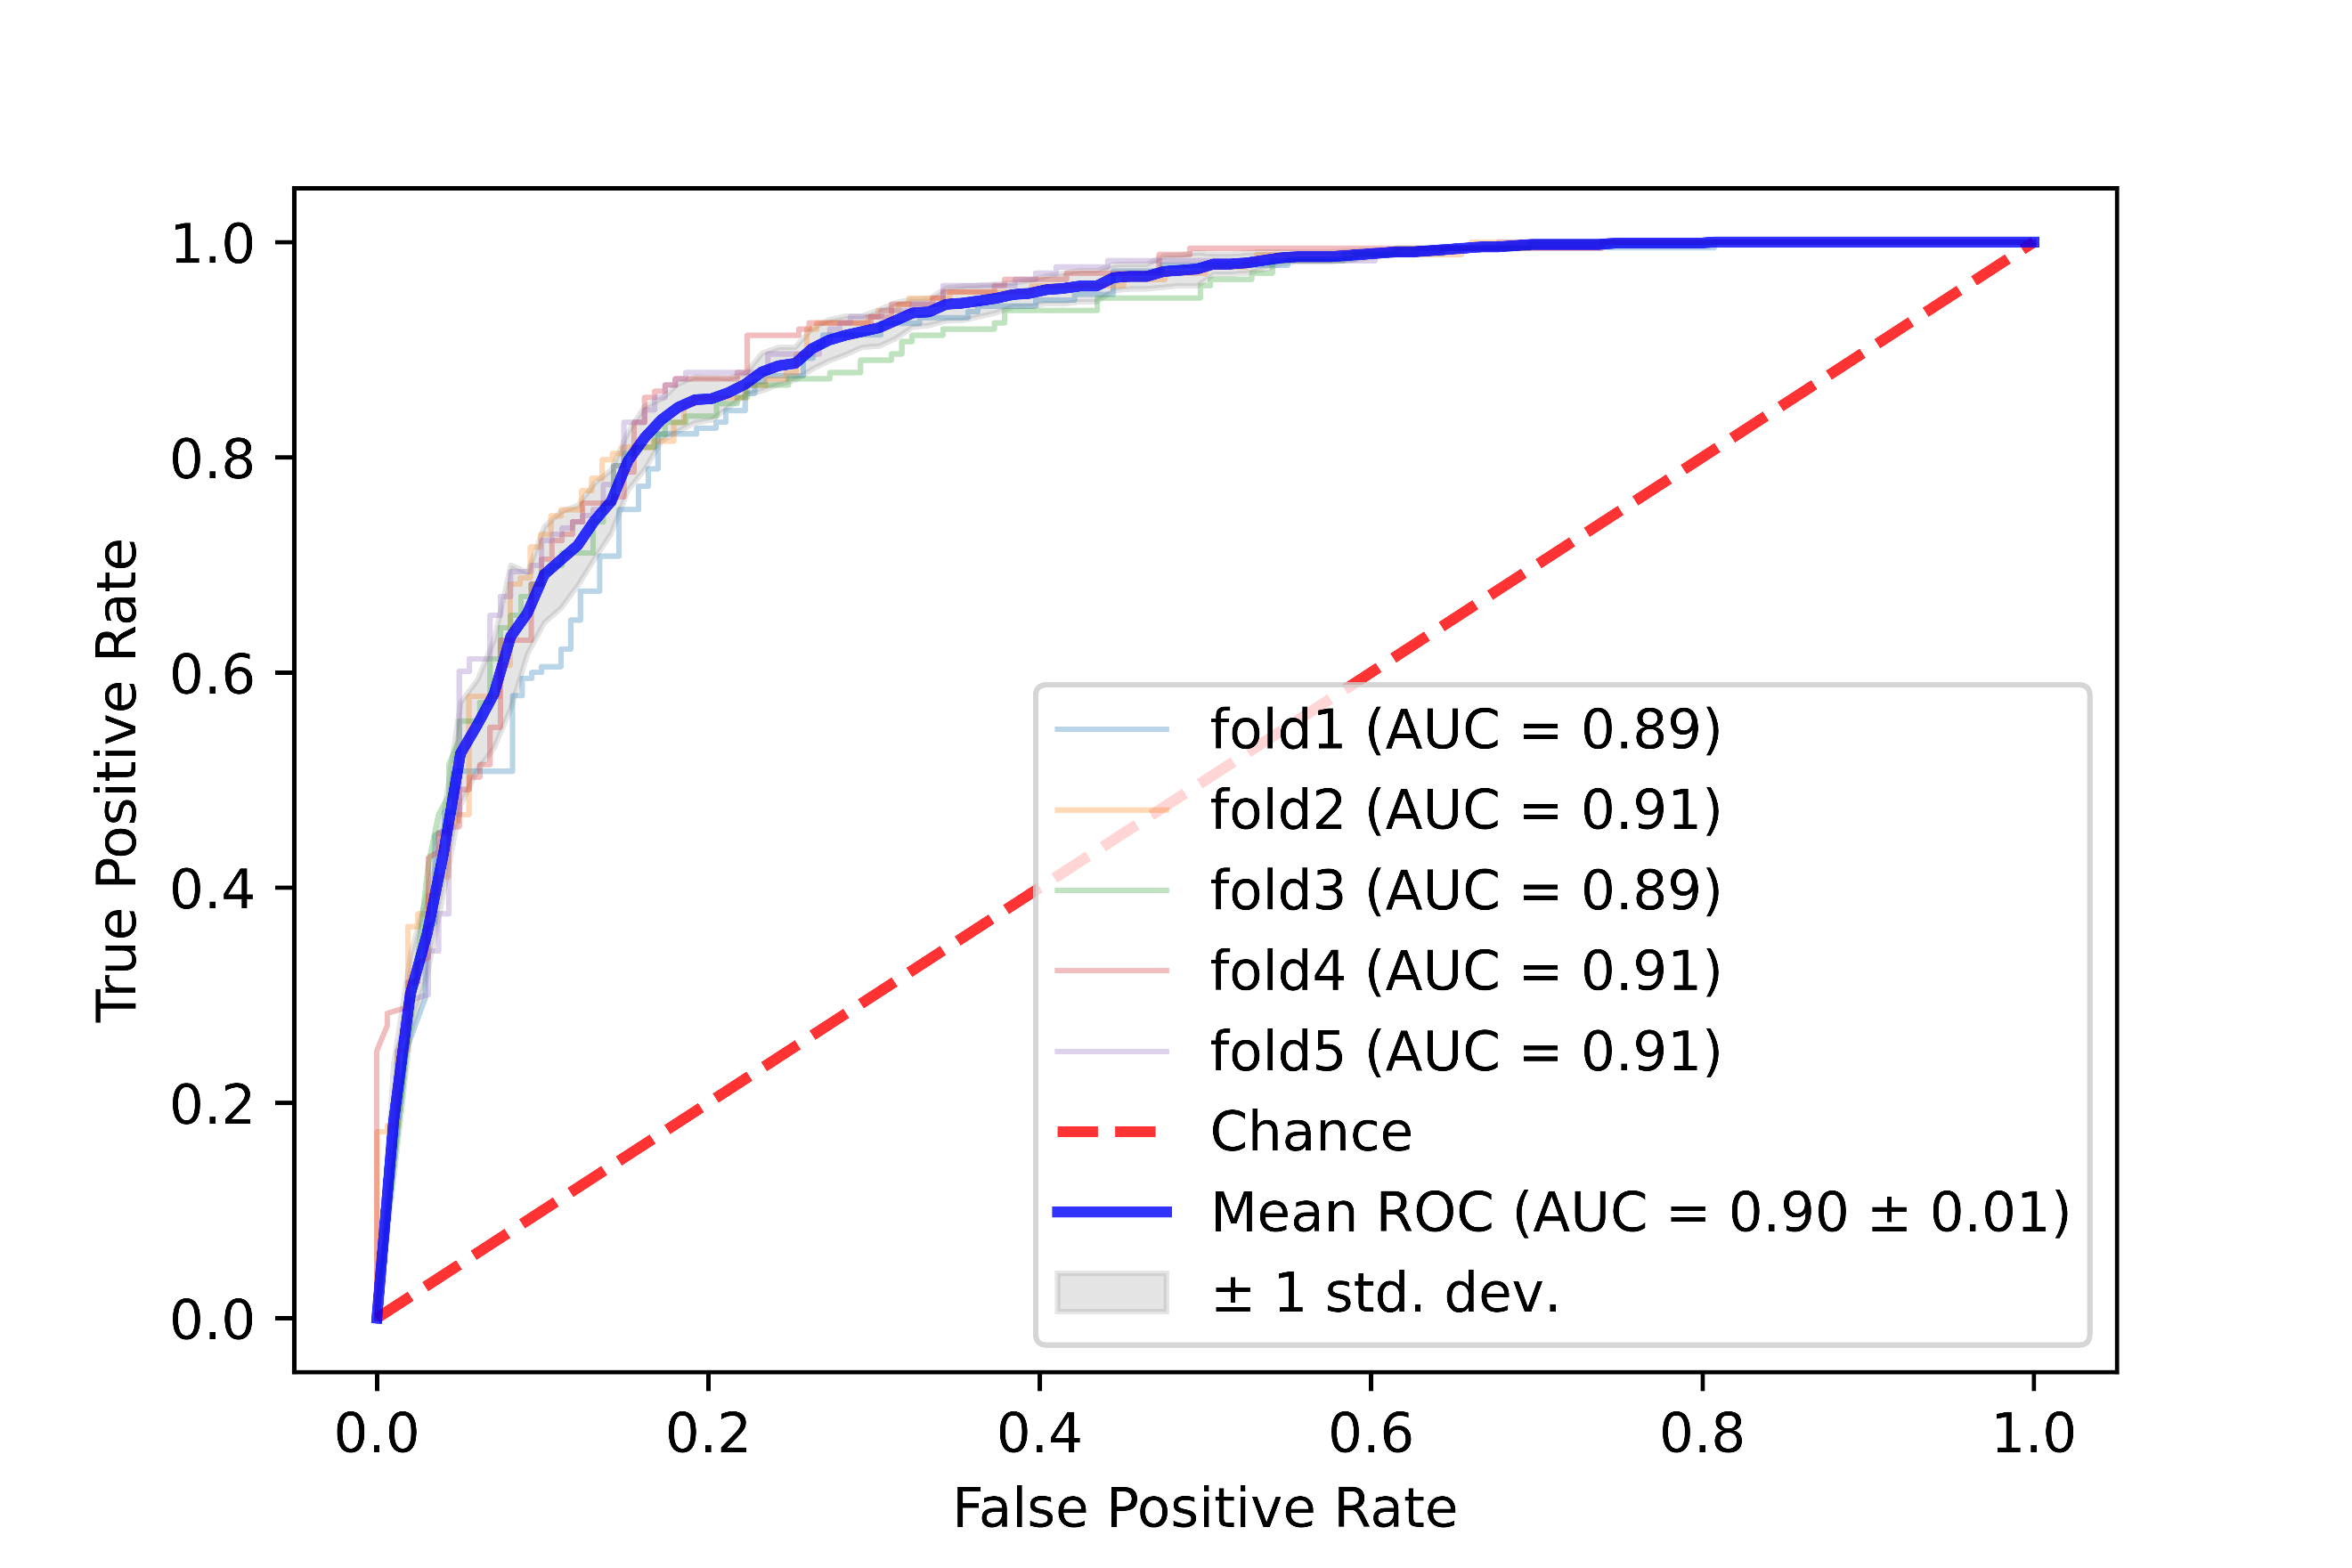
\includegraphics[width=\textwidth,keepaspectratio]{images/Supplement4/image1.png}
		\caption{ROC curve.}
	\end{subfigure}
	\hfill
	\begin{subfigure}[b]{0.49\textwidth}
		\centering
		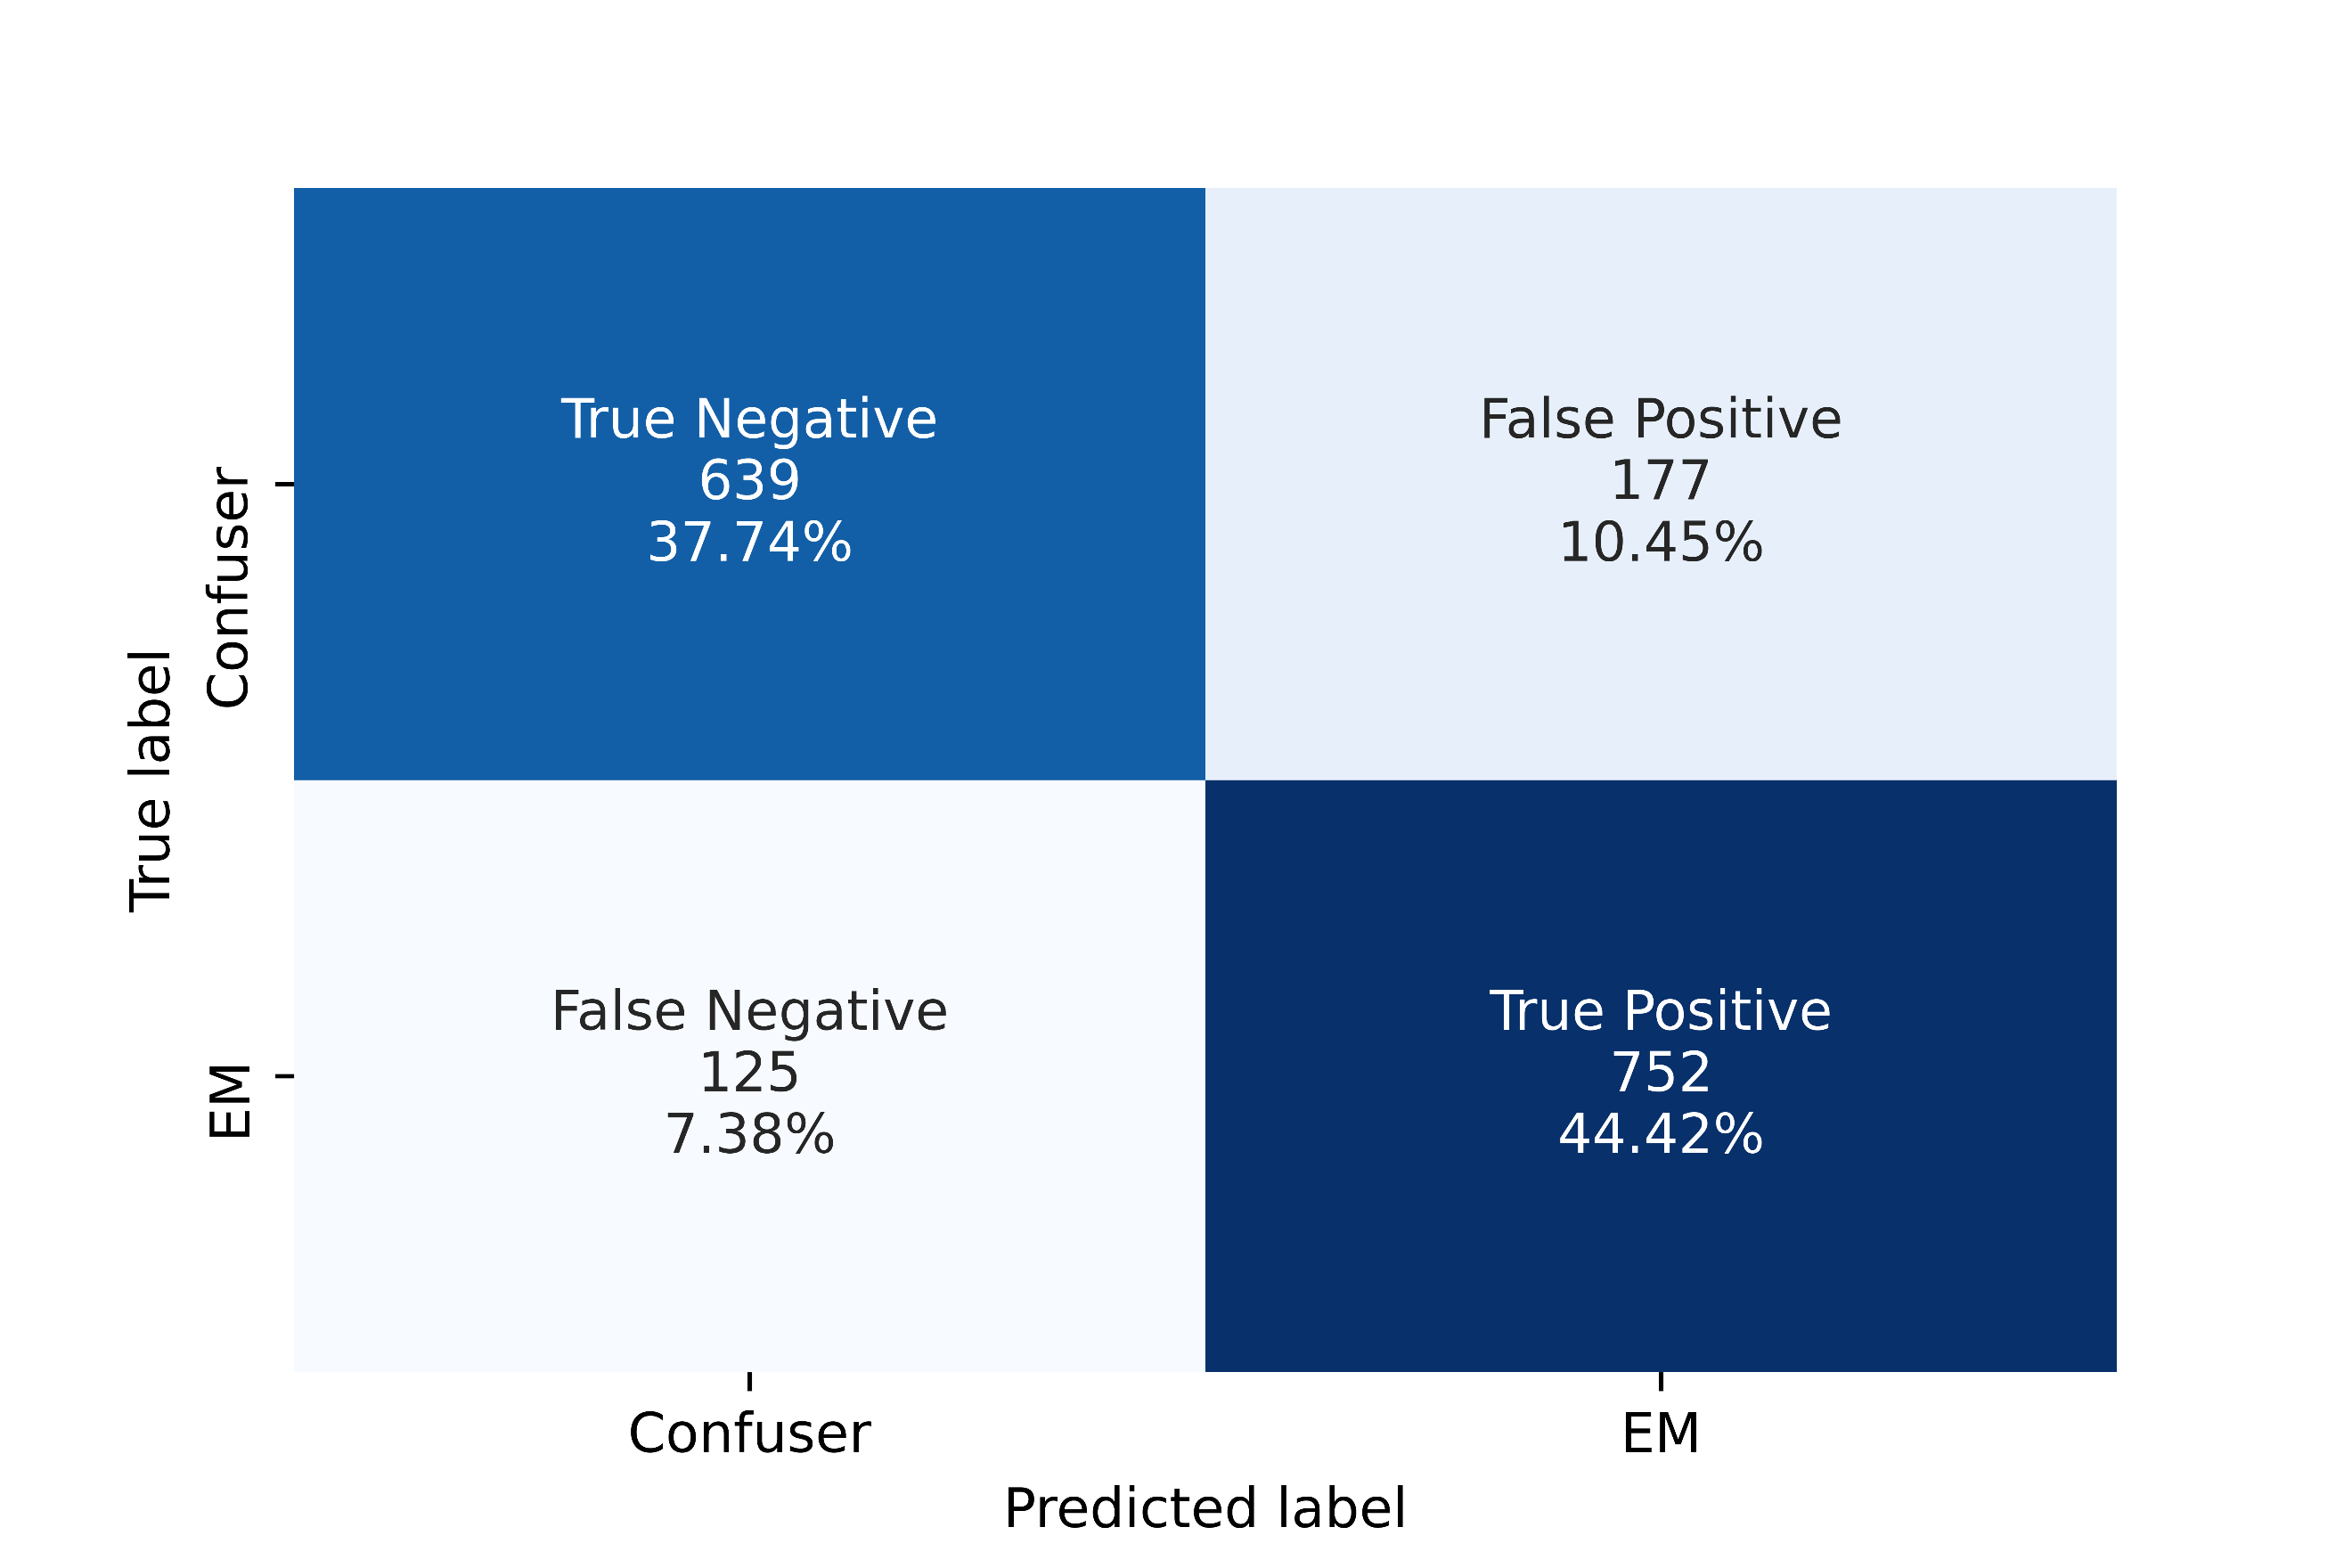
\includegraphics[width=\textwidth,keepaspectratio]{images/Supplement4/image7.png}
		\caption{Confusion matrix.}
	\end{subfigure}
	\caption{Five-fold cross-validation ROC curve and confusion matrix of VGG16-8 model.}
\end{figure}

%%%%%%%%%%%%%%Break%%%%%%%%%%%%%%%%%%%%%%
\vfill\clearpage
\subsection{VGG19-13}

\begin{table}[h!]
	\centering
	\caption{Five-fold cross-validation performance metrics of VGG19-13 model.}
	\resizebox{\textwidth}{!}{%
		\begin{tabular}{llllllllllll}
			\toprule
			& \multicolumn{11}{c}{\textbf{Metric}}    \\ \cmidrule(lr){2-12} 
			\multicolumn{1}{l}{\textbf{Fold}} & \rotatebox{45}{Accuracy} & \rotatebox{45}{Sensitivity} & \rotatebox{45}{Specificity} & \rotatebox{45}{Precision} & \rotatebox{45}{NPV} & \rotatebox{45}{MCC} & \rotatebox{45}{Kappa} & \rotatebox{45}{LR$+$} & \rotatebox{45}{LR$-$} & \rotatebox{45}{F1-Score} & \rotatebox{45}{AUC}  \\ \midrule
			fold1          & 81.74 & 85.41 & 77.78 & 80.61 & 83.12 & 0.6346 & 0.6334 & 3.8432 & 0.1876 & 0.8294 & 0.907  \\
			fold2          & 84.18 & 84.97 & 83.33 & 84.48 & 83.85 & 0.6832 & 0.6832 & 5.0983 & 0.1803 & 0.8473 & 0.9079 \\
			fold3          & 83.83 & 83.82 & 83.85 & 84.8  & 82.82 & 0.6764 & 0.6764 & 5.1901 & 0.193  & 0.843  & 0.9069 \\
			fold4          & 84.13 & 83.82 & 84.47 & 85.29 & 82.93 & 0.6825 & 0.6824 & 5.3977 & 0.1916 & 0.8455 & 0.9176 \\
			fold5          & 86.83 & 88.44 & 85.09 & 86.44 & 87.26 & 0.7362 & 0.736  & 5.9328 & 0.1359 & 0.8743 & 0.9254 \\ \cmidrule(lr){1-12} 
			average        & 84.14 & 85.29 & 82.9  & 84.32 & 84    & 0.6826 & 0.6823 & 5.0924 & 0.1777 & 0.8479 & 0.913  \\
			std. deviation & 1.62  & 1.69  & 2.63  & 1.97  & 1.67  & 0.0323 & 0.0326 & 0.6884 & 0.0214 & 0.0146 & 0.0074\\
			\bottomrule
		\end{tabular}%
	}
\end{table}


\begin{figure}[h!]
	\centering
	\begin{subfigure}[b]{0.49\textwidth}
		\centering
		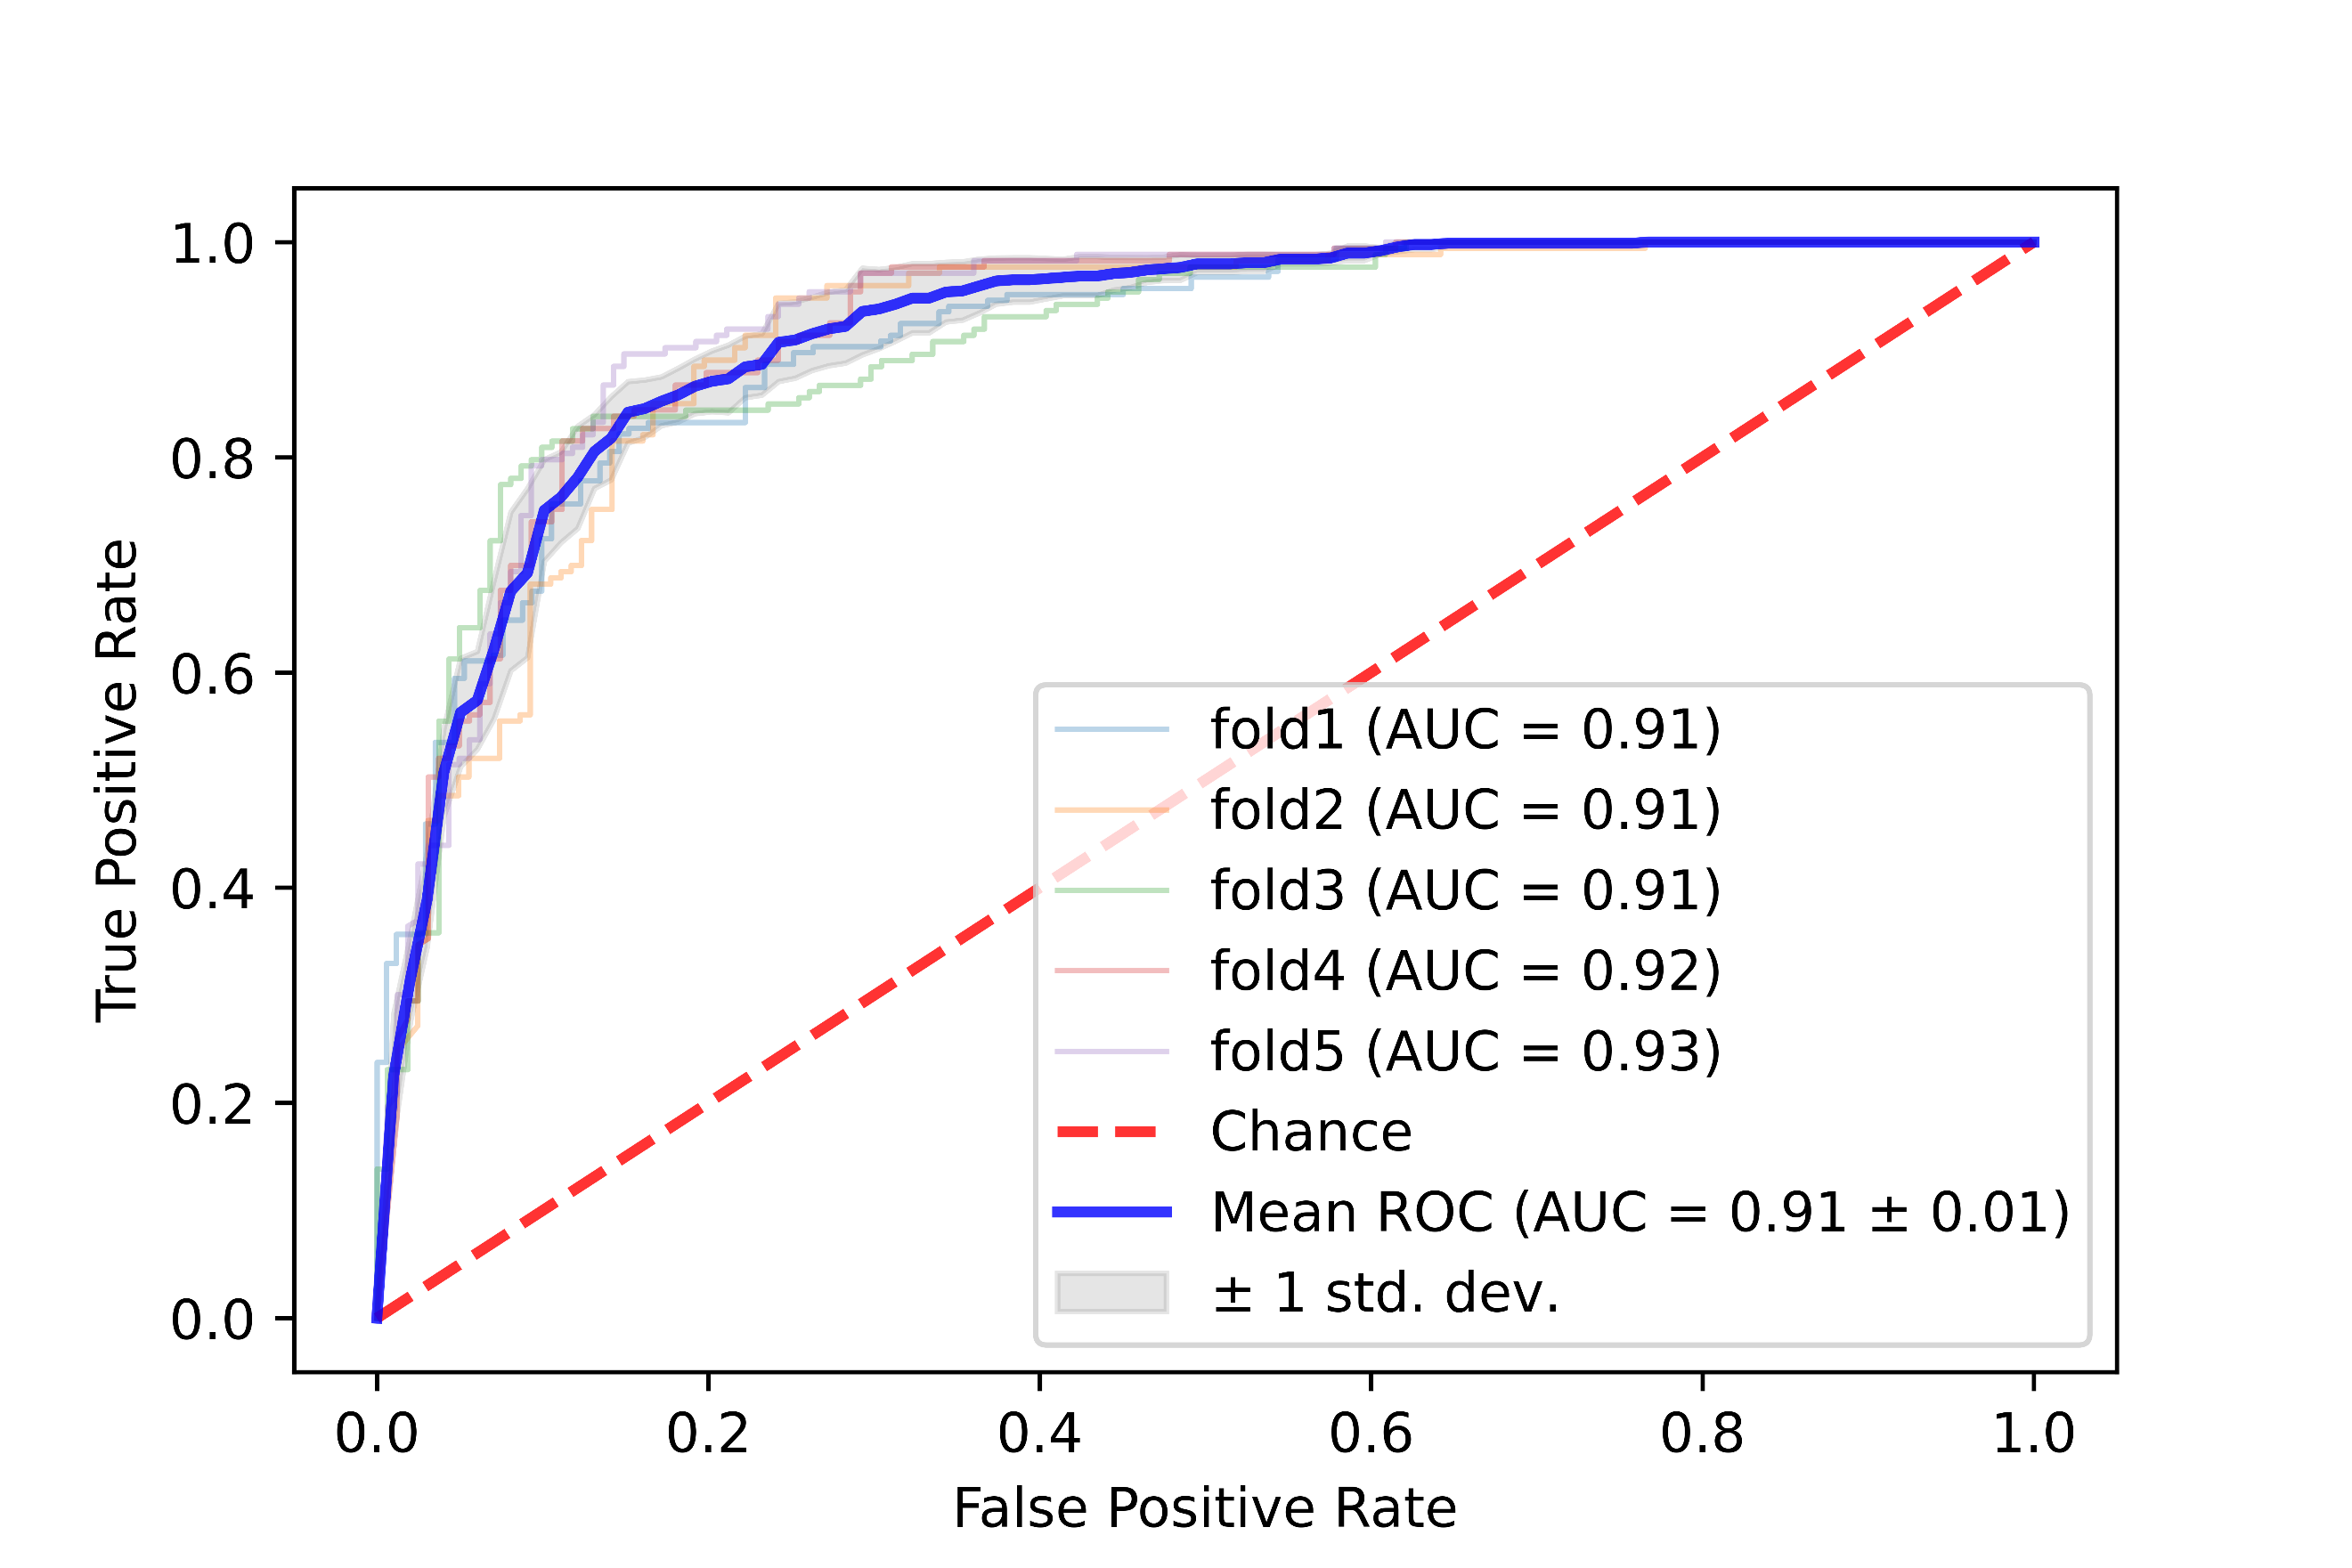
\includegraphics[width=\textwidth,keepaspectratio]{images/Supplement4/image8.png}
		\caption{ROC curve.}
	\end{subfigure}
	\hfill
	\begin{subfigure}[b]{0.49\textwidth}
		\centering
		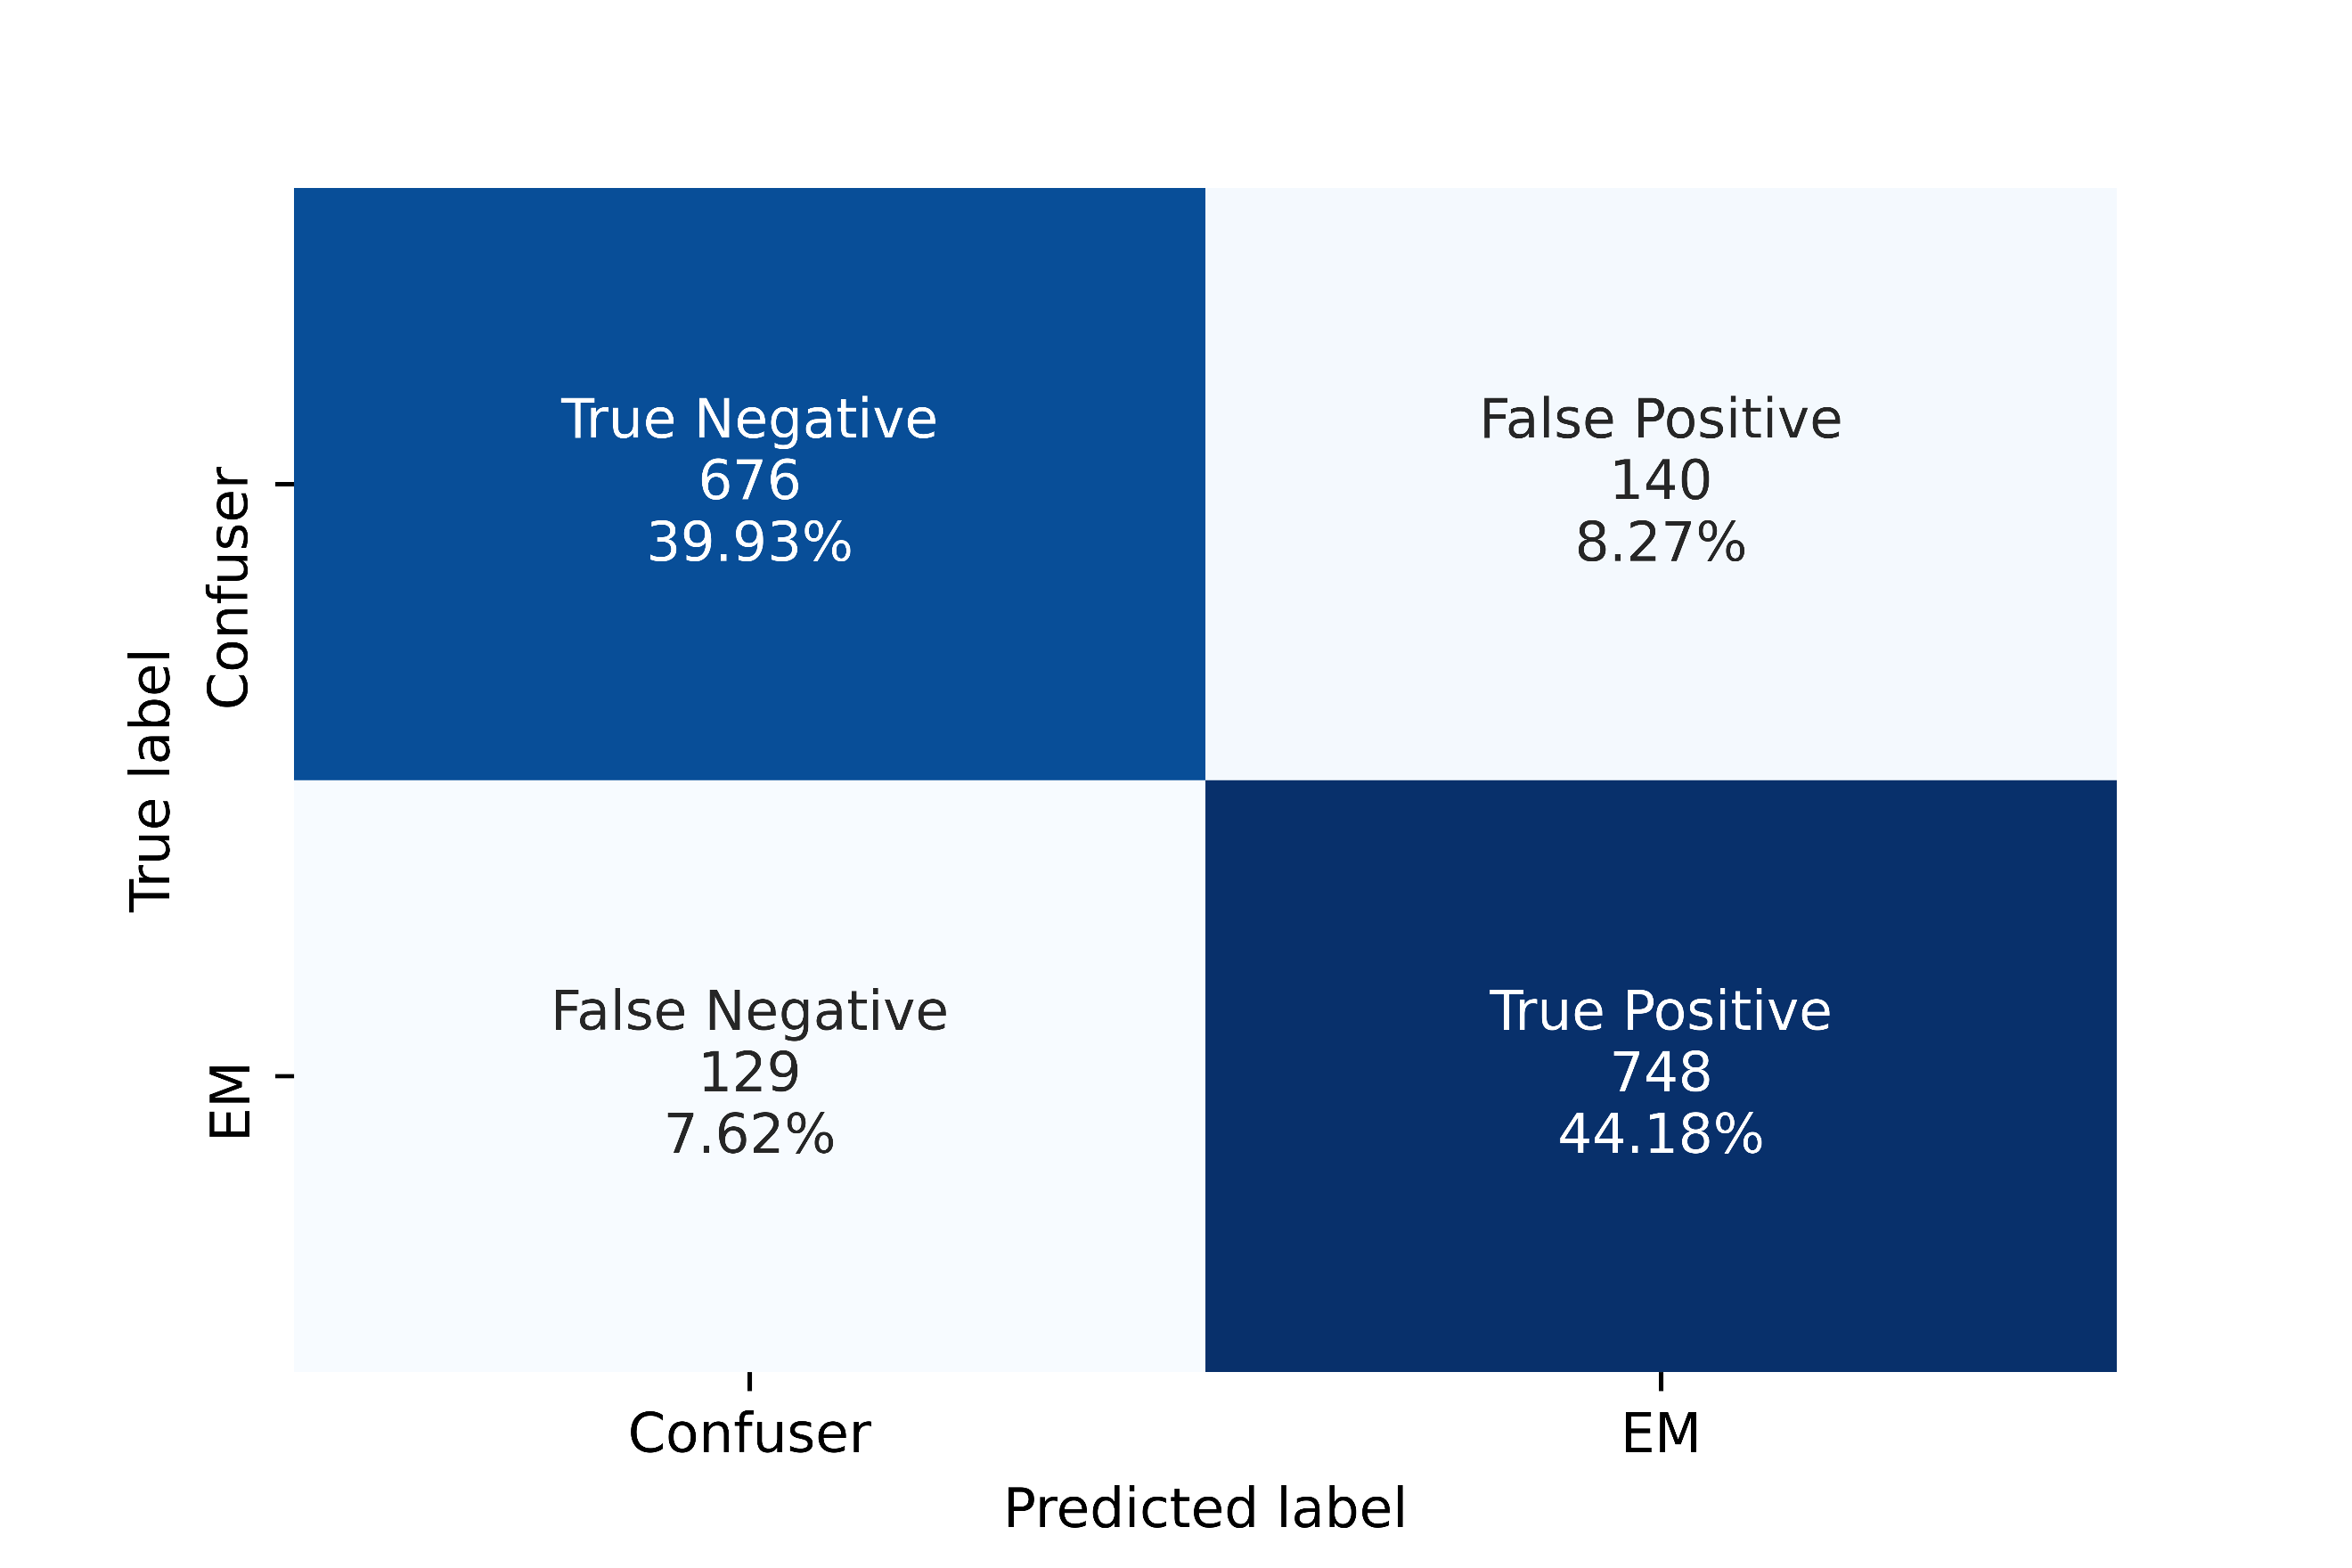
\includegraphics[width=\textwidth,keepaspectratio]{images/Supplement4/image13.png}
		\caption{Confusion matrix.}
	\end{subfigure}
	\caption{Five-fold cross-validation ROC curve and confusion matrix of VGG19-13 model.}
\end{figure}

%%%%%%%%%%%%%%Break%%%%%%%%%%%%%%%%%%%%%%
\vfill\clearpage
\subsection{ResNet50-Burlina}

\begin{table}[h!]
	\centering
	\caption{Performance metrics of ResNet50-Burlina models\tablefootnote{\url{https://github.com/neil454/lyme-1600-model} (visited on 02/20/2023).} trained by Burlina et al. \cite{Burlina2018} tested on the whole dataset of this study.}
	\resizebox{\textwidth}{!}{%
		\begin{tabular}{llllllllllll}
			\toprule
			& \multicolumn{11}{c}{\textbf{Metric}}    \\ \cmidrule(lr){2-12} 
			\multicolumn{1}{l}{\textbf{Model}} & \rotatebox{45}{Accuracy} 
			& \rotatebox{45}{Sensitivity} & \rotatebox{45}{Specificity} 
			& \rotatebox{45}{Precision} & \rotatebox{45}{NPV} & \rotatebox{45}{MCC} 
			& \rotatebox{45}{Kappa} 
			& \rotatebox{45}{LR$+$} & \rotatebox{45}{LR$-$} & \rotatebox{45}{F1-Score} 
			& \rotatebox{45}{AUC}  \\ \midrule
			fold1          & 75.12 & 65.7  & 85.24 & 82.7  & 69.82 & 0.5172 & 0.5055 & 4.4502 & 0.4024 & 0.7323 & 0.4646 \\
			fold2          & 75.6  & 74.48 & 76.8  & 77.52 & 73.69 & 0.5125 & 0.512  & 3.2102 & 0.3323 & 0.7597 & 0.5589 \\
			fold3          & 75.72 & 66.4  & 85.73 & 83.33 & 70.37 & 0.5291 & 0.5174 & 4.6536 & 0.392  & 0.7391 & 0.4143 \\
			fold4          & 76.67 & 69.98 & 83.87 & 82.34 & 72.22 & 0.542  & 0.5355 & 4.3386 & 0.358  & 0.7566 & 0.4509 \\
			fold5          & 77.15 & 73.67 & 80.89 & 80.56 & 74.09 & 0.5461 & 0.5439 & 3.8558 & 0.3255 & 0.7696 & 0.5162 \\ \cmidrule(lr){1-12}
			average        & 76.05 & 70.05 & 82.51 & 81.29 & 72.04 & 0.5294 & 0.5229 & 4.1017 & 0.362  & 0.7515 & 0.481  \\
			std. deviation & 0.74  & 3.6   & 3.31  & 2.1   & 1.71  & 0.0132 & 0.0145 & 0.5172 & 0.0309 & 0.0137 & 0.0509\\
			\bottomrule
		\end{tabular}%
	}
\end{table}


\begin{figure}[h!]
	\centering
	\begin{subfigure}[b]{0.49\textwidth}
		\centering
		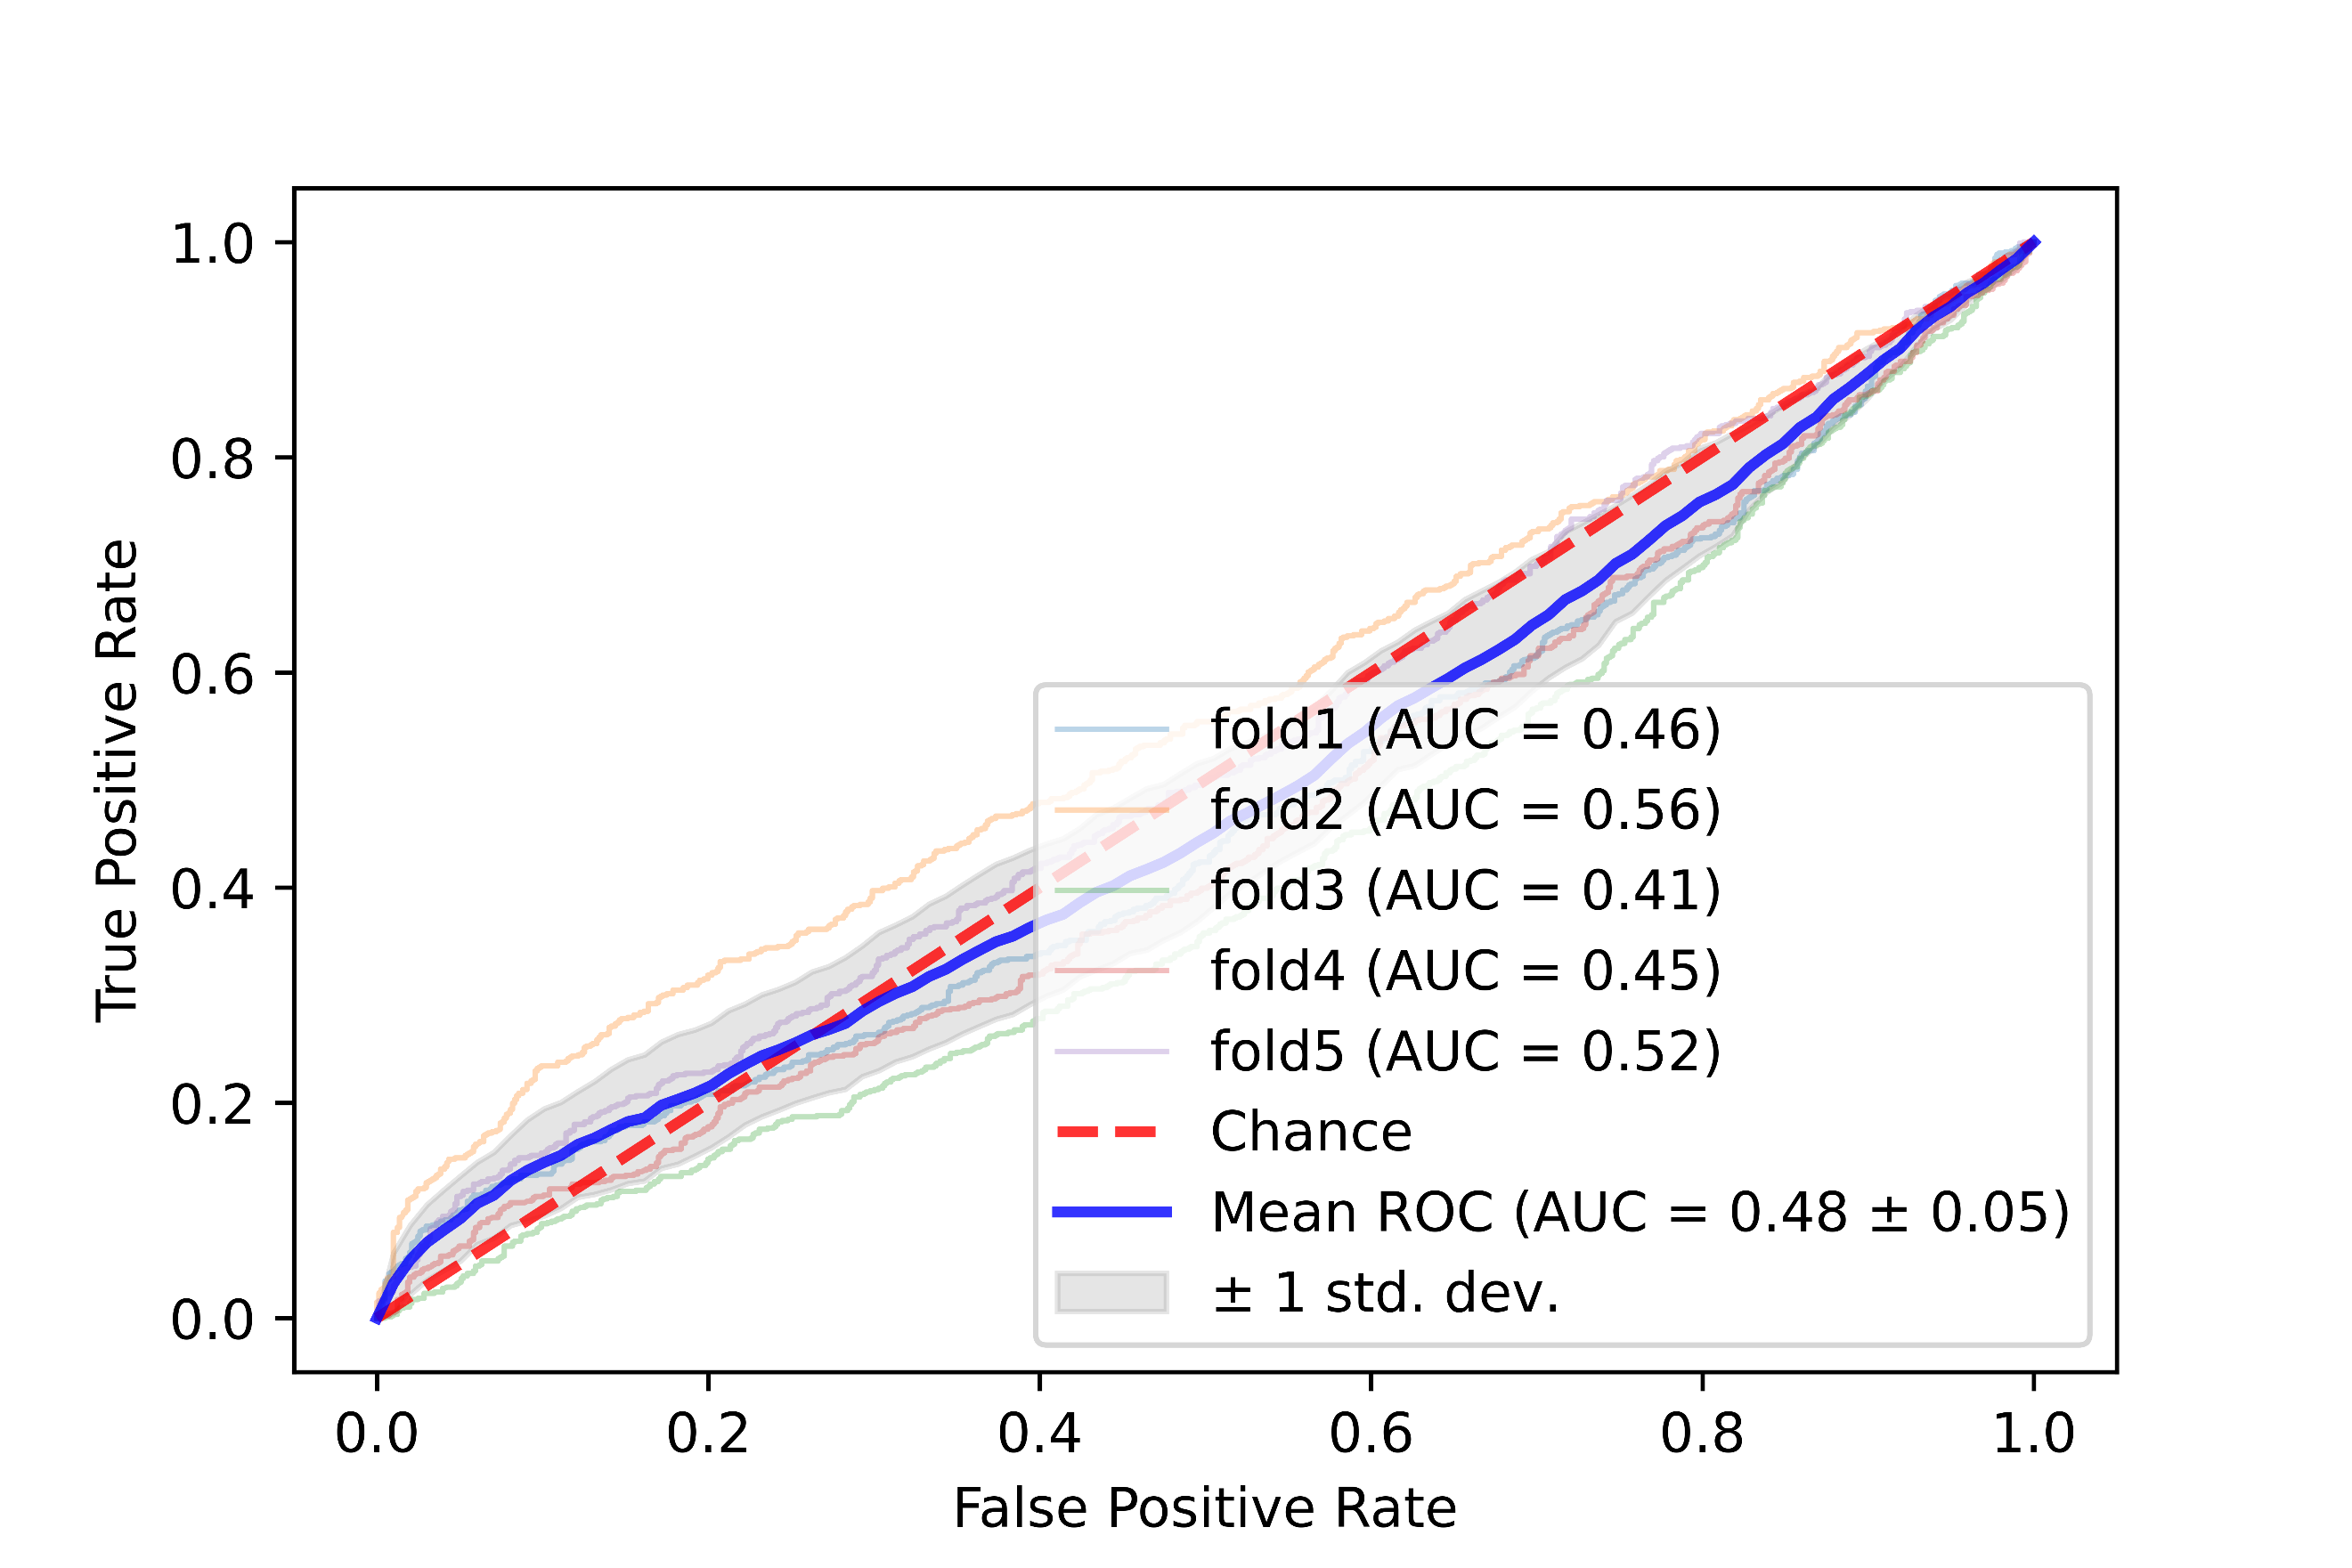
\includegraphics[width=\textwidth,keepaspectratio]{images/Supplement4/image14.png}
		\caption{ROC curve.}
	\end{subfigure}
	\hfill
	\begin{subfigure}[b]{0.49\textwidth}
		\centering
		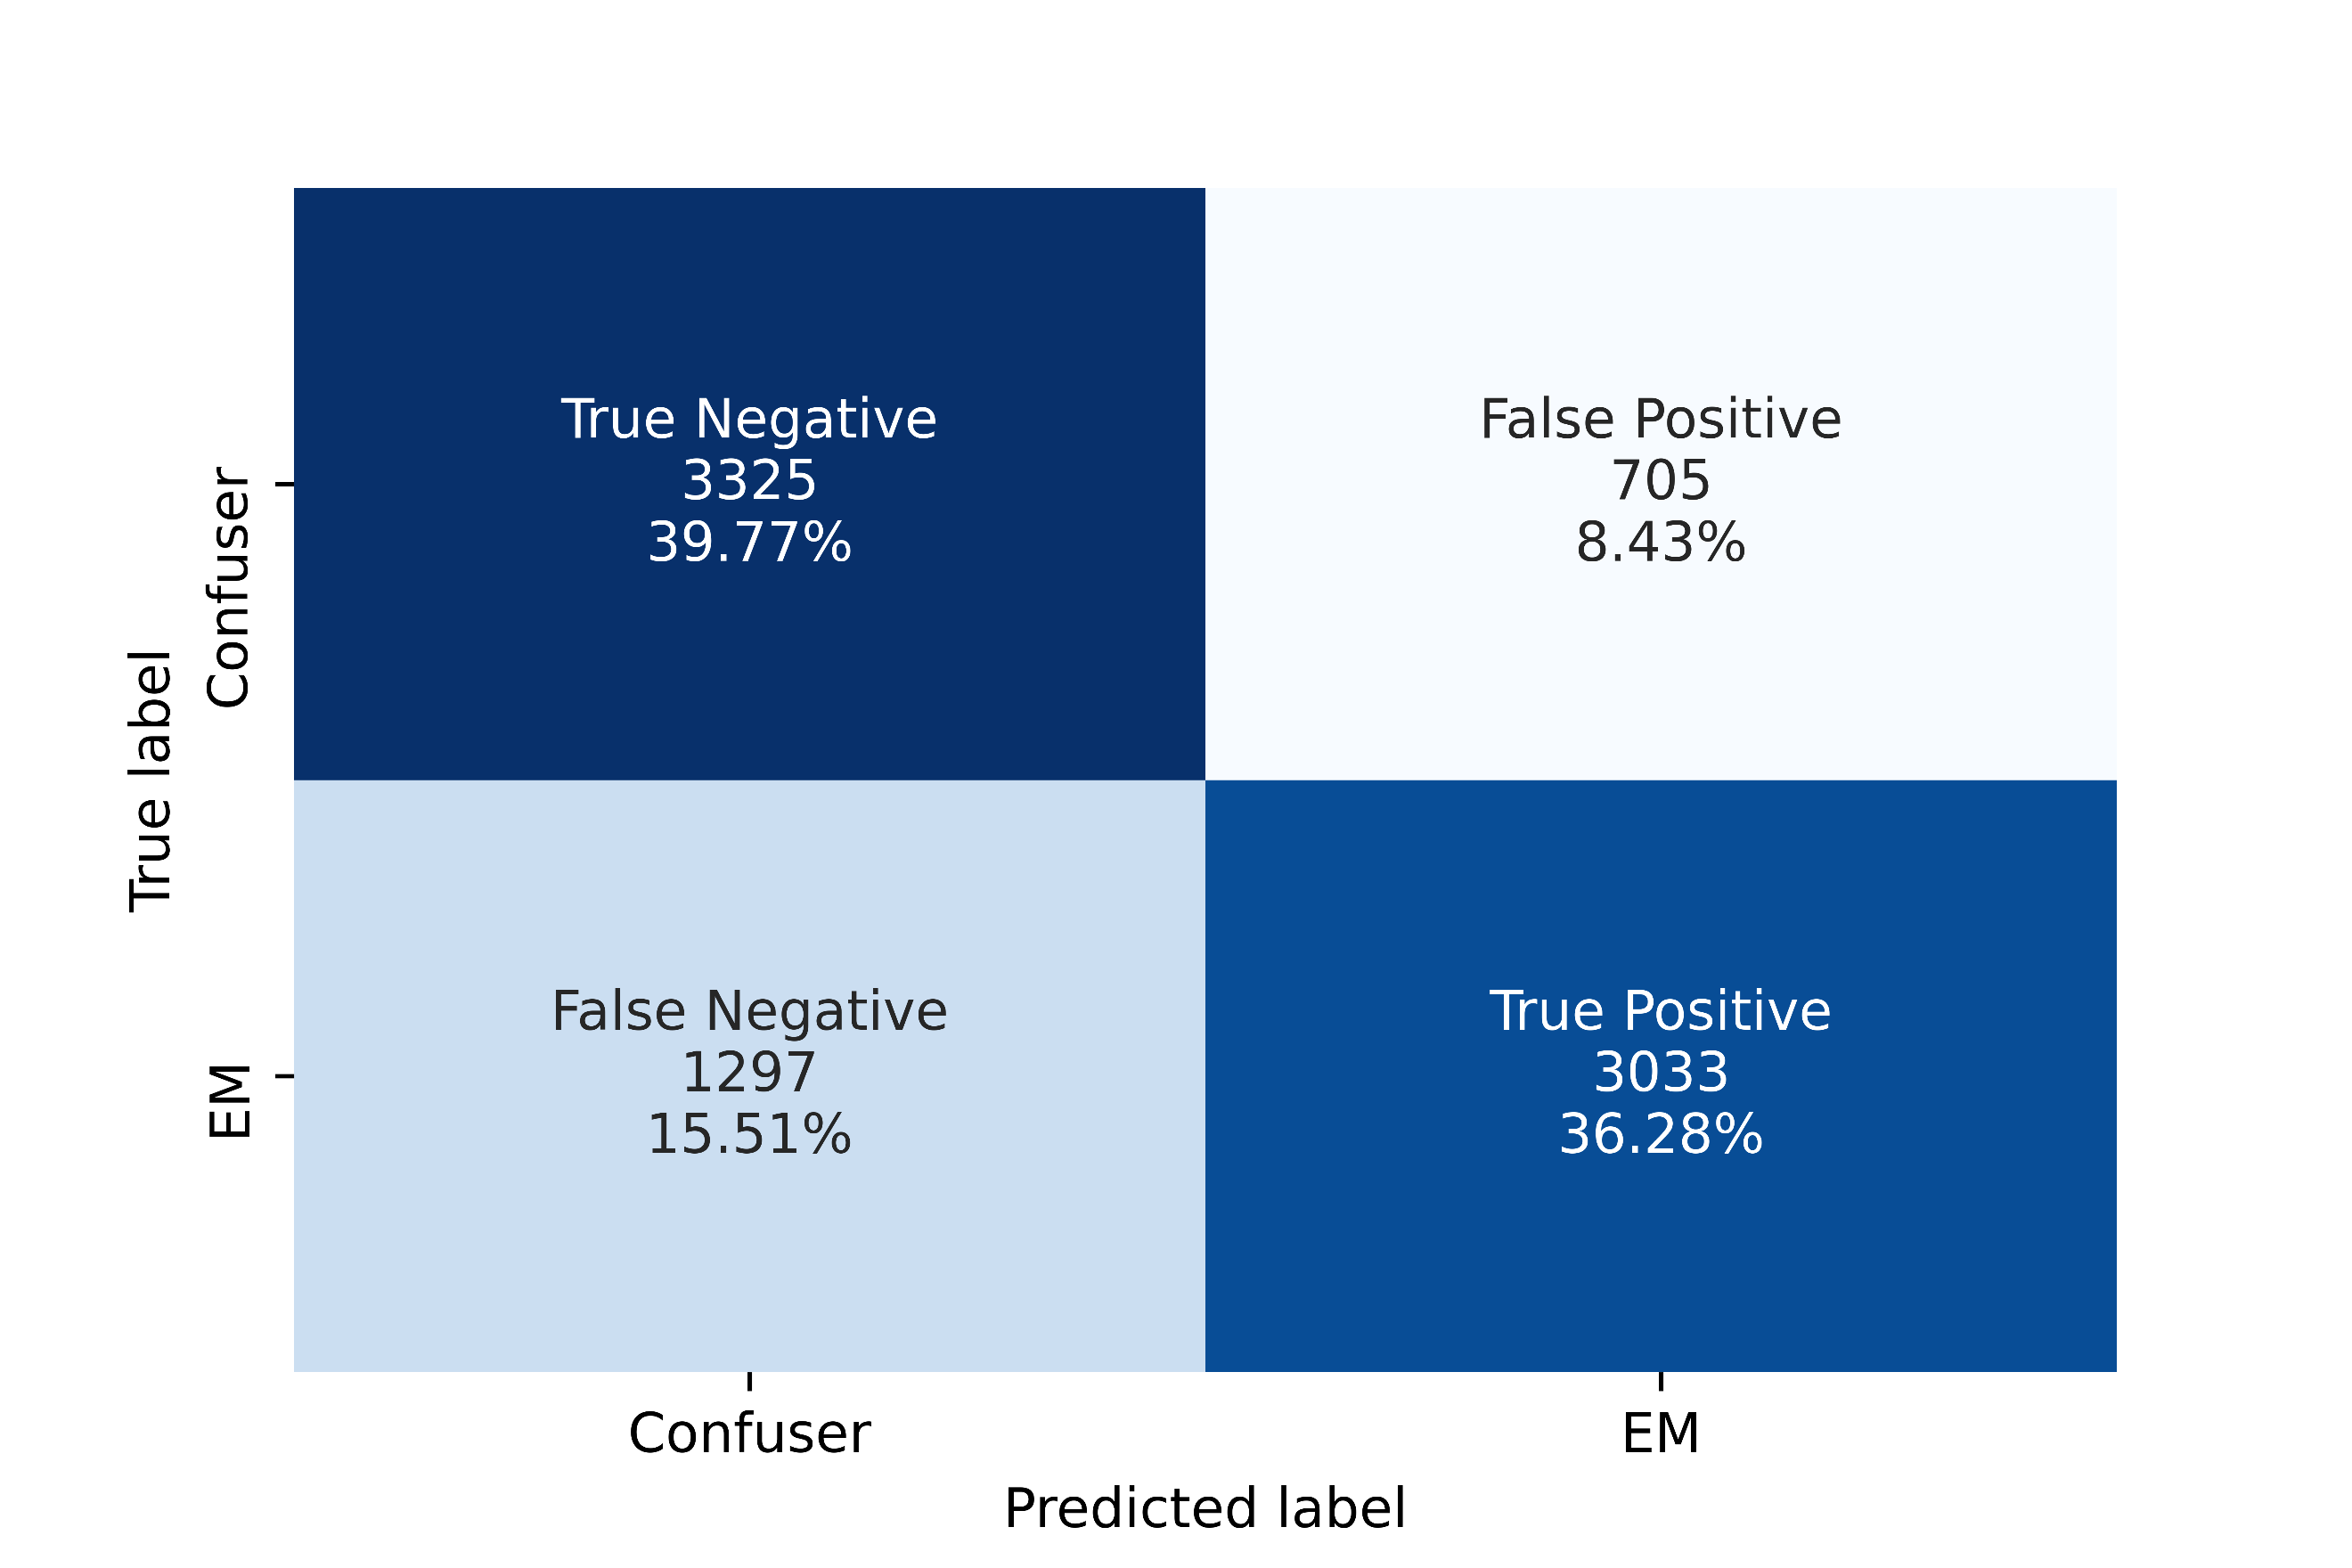
\includegraphics[width=\textwidth,keepaspectratio]{images/Supplement4/image20.png}
		\caption{Confusion matrix.}
	\end{subfigure}
	\caption{ROC curve and confusion matrix of ResNet50-Burlina models trained by Burlina et al. \cite{Burlina2018} tested on the whole dataset of this study.}
\end{figure}

%%%%%%%%%%%%%%Break%%%%%%%%%%%%%%%%%%%%%%
\vfill\clearpage
\subsection{ResNet50-NoAug}

\begin{table}[h!]
	\centering
	\caption{Five-fold cross-validation performance metrics of ResNet50-NoAug model.}
	\resizebox{\textwidth}{!}{%
		\begin{tabular}{llllllllllll}
			\toprule
			& \multicolumn{11}{c}{\textbf{Metric}}    \\ \cmidrule(lr){2-12} 
			\multicolumn{1}{l}{\textbf{Fold}} & \rotatebox{45}{Accuracy} 
			& \rotatebox{45}{Sensitivity} & \rotatebox{45}{Specificity} 
			& \rotatebox{45}{Precision} & \rotatebox{45}{NPV} & \rotatebox{45}{MCC} 
			& \rotatebox{45}{Kappa} 
			& \rotatebox{45}{LR$+$} & \rotatebox{45}{LR$-$} & \rotatebox{45}{F1-Score} 
			& \rotatebox{45}{AUC}  \\ \midrule
			fold1          & 59.7  & 56.9  & 62.73 & 62.26 & 57.39 & 0.1964 & 0.1956 & 1.5267 & 0.6871 & 0.5946 & 0.6429 \\
			fold2          & 62.09 & 71.1  & 52.47 & 61.5  & 62.96 & 0.2401 & 0.2369 & 1.4958 & 0.5508 & 0.6595 & 0.6491 \\
			fold3          & 61.98 & 71.1  & 52.17 & 61.5  & 62.69 & 0.2372 & 0.2341 & 1.4866 & 0.5539 & 0.6595 & 0.6405 \\
			fold4          & 63.17 & 76.3  & 49.07 & 61.68 & 65.83 & 0.2642 & 0.2559 & 1.4981 & 0.483  & 0.6822 & 0.6915 \\
			fold5          & 60.18 & 83.24 & 35.4  & 58.06 & 66.28 & 0.213  & 0.1895 & 1.2886 & 0.4735 & 0.6841 & 0.6285 \\ \cmidrule(lr){1-12}
			average        & 61.42 & 71.73 & 50.37 & 61    & 63.03 & 0.2302 & 0.2224 & 1.4592 & 0.5497 & 0.656  & 0.6505 \\
			std. deviation & 1.29  & 8.65  & 8.79  & 1.5   & 3.17  & 0.0234 & 0.0256 & 0.0863 & 0.0764 & 0.0325 & 0.0216\\
			\bottomrule
		\end{tabular}%
	}
\end{table}


\begin{figure}[h!]
	\centering
	\begin{subfigure}[b]{0.49\textwidth}
		\centering
		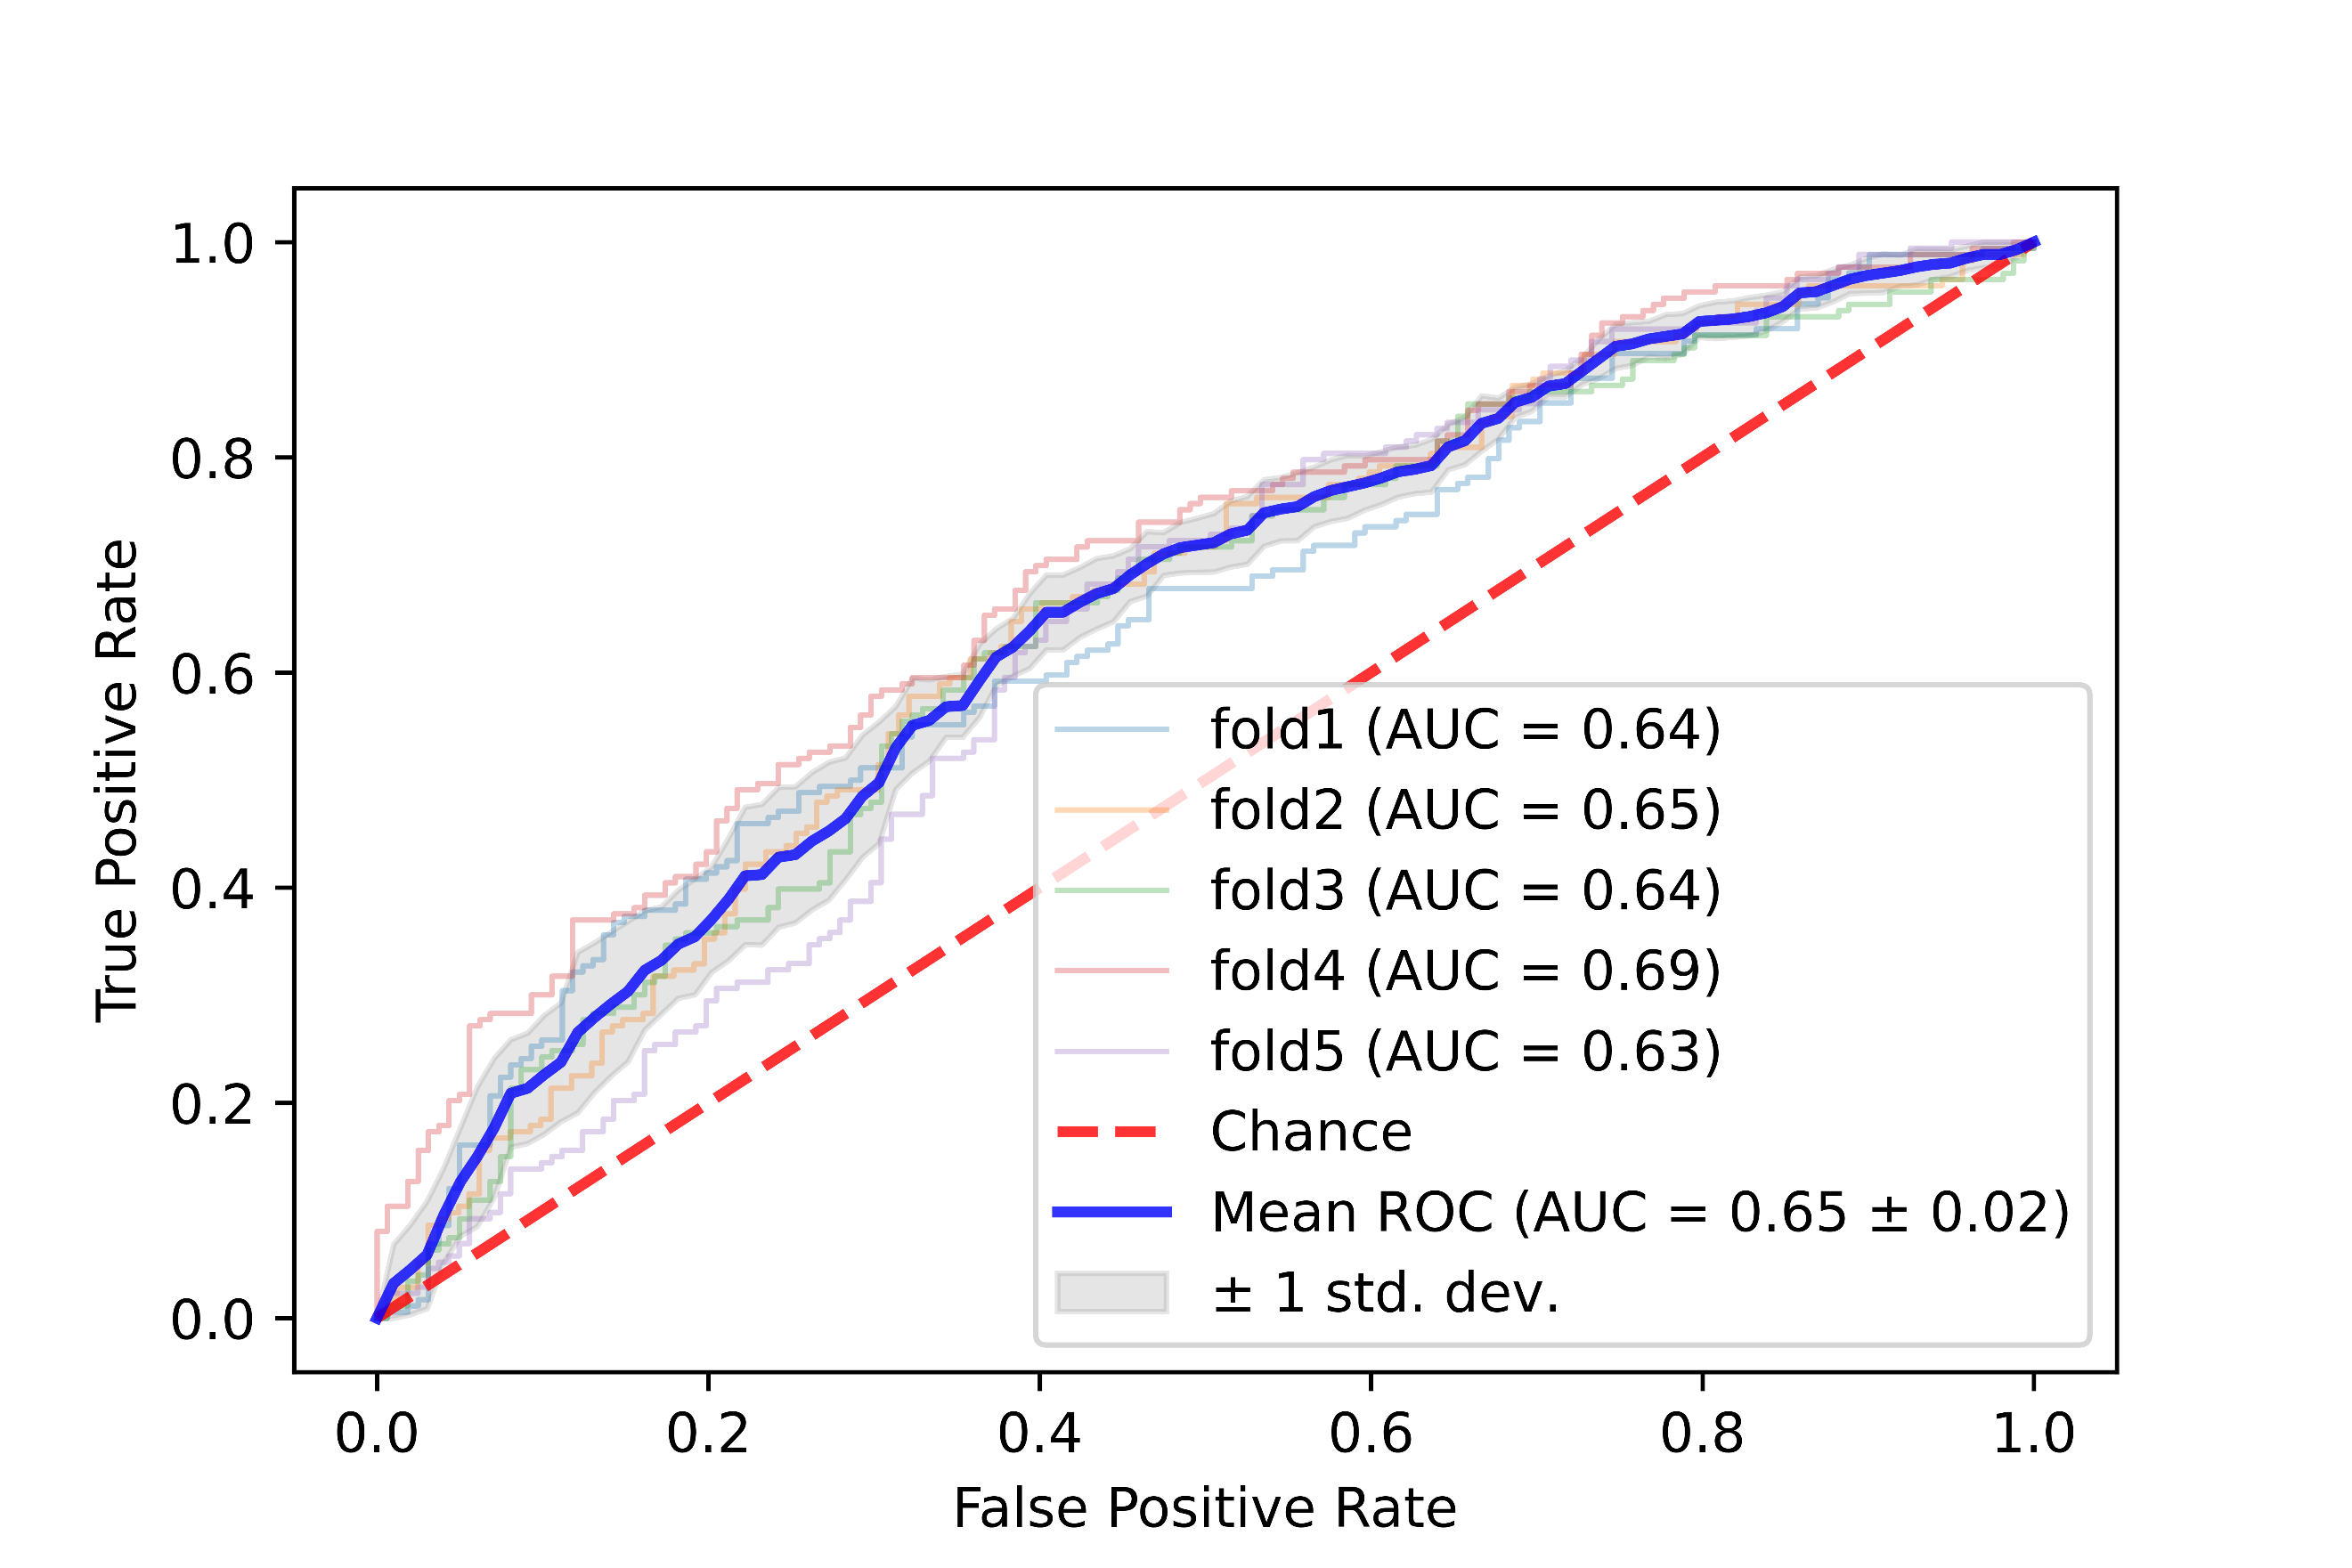
\includegraphics[width=\textwidth,keepaspectratio]{images/Supplement4/image21.png}
		\caption{ROC curve.}
	\end{subfigure}
	\hfill
	\begin{subfigure}[b]{0.49\textwidth}
		\centering
		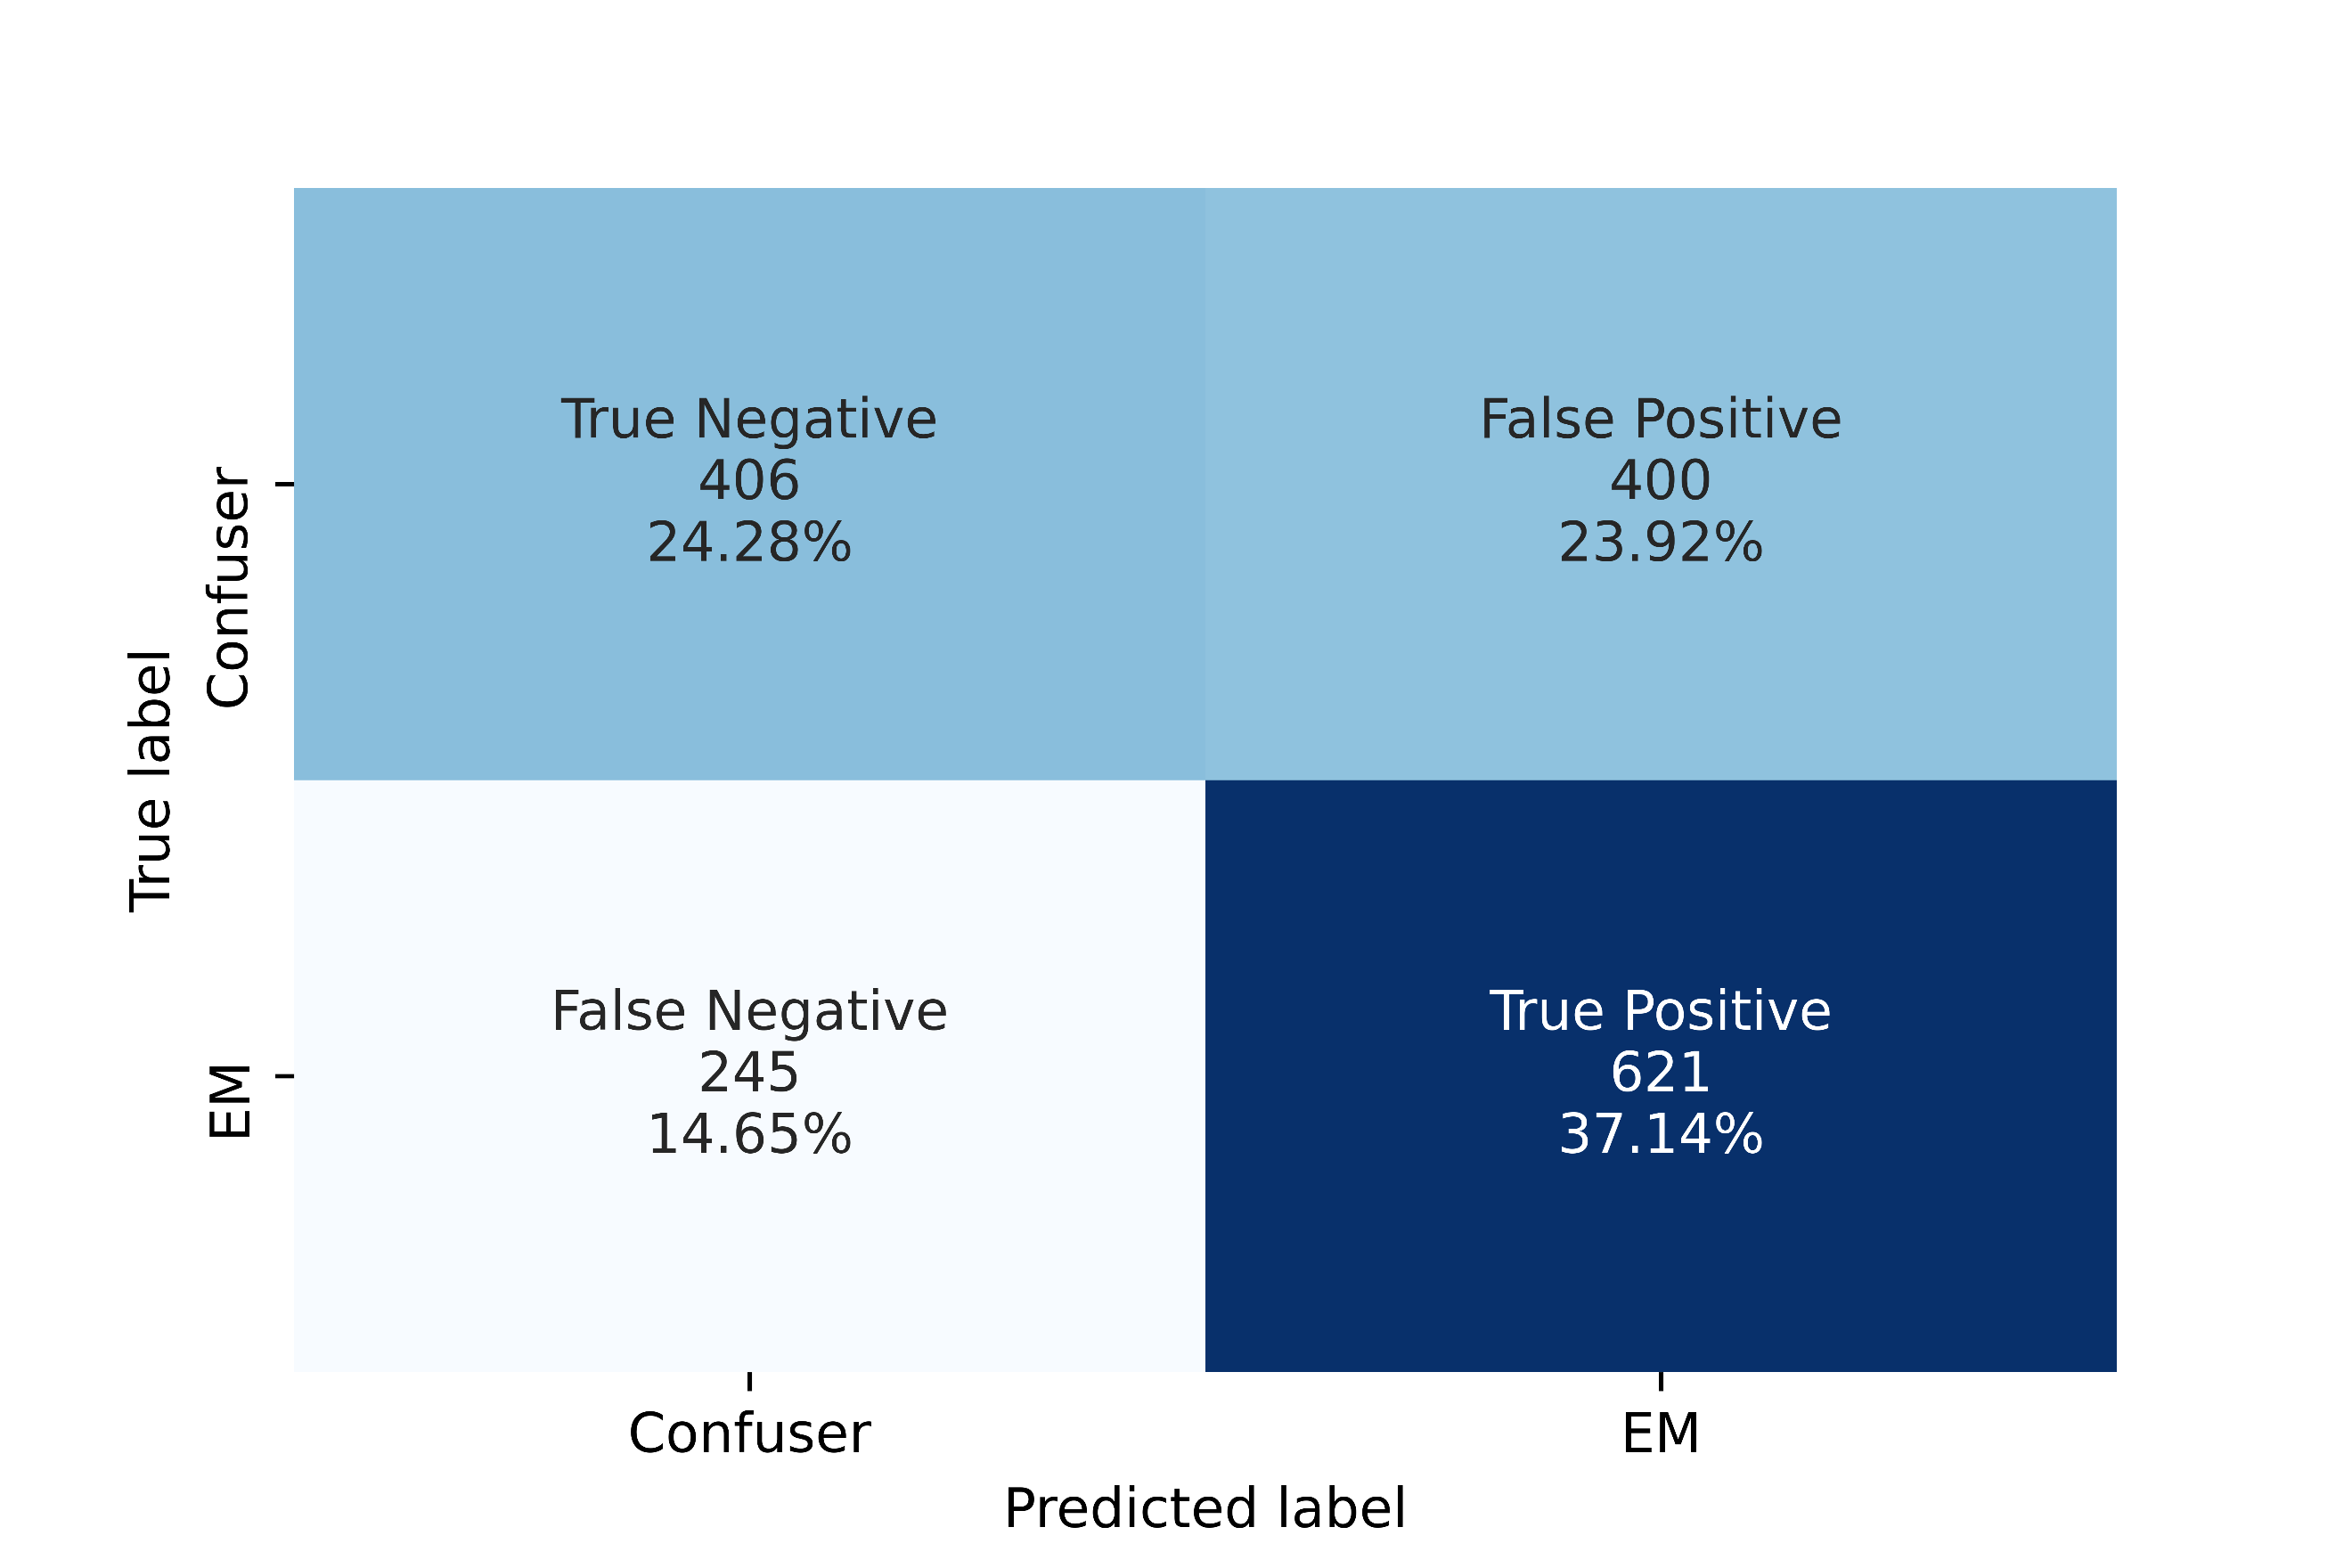
\includegraphics[width=\textwidth,keepaspectratio]{images/Supplement4/image27.png}
		\caption{Confusion matrix.}
	\end{subfigure}
	\caption{Five-fold cross-validation ROC curve and confusion matrix of ResNet50-NoAug model.}
\end{figure}

%%%%%%%%%%%%%%Break%%%%%%%%%%%%%%%%%%%%%%
\vfill\clearpage
\subsection{ResNet50-NTL}

\begin{table}[h!]
	\centering
	\caption{Five-fold cross-validation performance metrics of ResNet50-NTL model.}
	\resizebox{\textwidth}{!}{%
		\begin{tabular}{llllllllllll}
			\toprule
			& \multicolumn{11}{c}{\textbf{Metric}}    \\ \cmidrule(lr){2-12} 
			\multicolumn{1}{l}{\textbf{Fold}} & \rotatebox{45}{Accuracy} 
			& \rotatebox{45}{Sensitivity} & \rotatebox{45}{Specificity} 
			& \rotatebox{45}{Precision} & \rotatebox{45}{NPV} & \rotatebox{45}{MCC} 
			& \rotatebox{45}{Kappa} 
			& \rotatebox{45}{LR$+$} & \rotatebox{45}{LR$-$} & \rotatebox{45}{F1-Score} 
			& \rotatebox{45}{AUC}  \\ \midrule
			fold1          & 78.09 & 83.78 & 71.93 & 76.35 & 80.39 & 0.5623 & 0.5594 & 2.9848 & 0.2254 & 0.799  & 0.8565 \\
			fold2          & 77.01 & 79.77 & 74.07 & 76.67 & 77.42 & 0.5396 & 0.5392 & 3.0768 & 0.2731 & 0.7819 & 0.8342 \\
			fold3          & 76.05 & 82.66 & 68.94 & 74.09 & 78.72 & 0.5221 & 0.5183 & 2.6616 & 0.2515 & 0.7814 & 0.8423 \\
			fold4          & 71.86 & 61.85 & 82.61 & 79.26 & 66.83 & 0.4527 & 0.441  & 3.5564 & 0.4618 & 0.6948 & 0.8248 \\
			fold5          & 78.74 & 84.39 & 72.67 & 76.84 & 81.25 & 0.5758 & 0.5727 & 3.088  & 0.2148 & 0.8044 & 0.8776 \\ \cmidrule(lr){1-12}
			average        & 76.35 & 78.49 & 74.04 & 76.64 & 76.92 & 0.5305 & 0.5261 & 3.0735 & 0.2853 & 0.7723 & 0.8471 \\
			std. deviation & 2.43  & 8.47  & 4.6   & 1.64  & 5.22  & 0.0431 & 0.0464 & 0.2867 & 0.0906 & 0.0398 & 0.0185\\
			\bottomrule
		\end{tabular}%
	}
\end{table}


\begin{figure}[h!]
	\centering
	\begin{subfigure}[b]{0.49\textwidth}
		\centering
		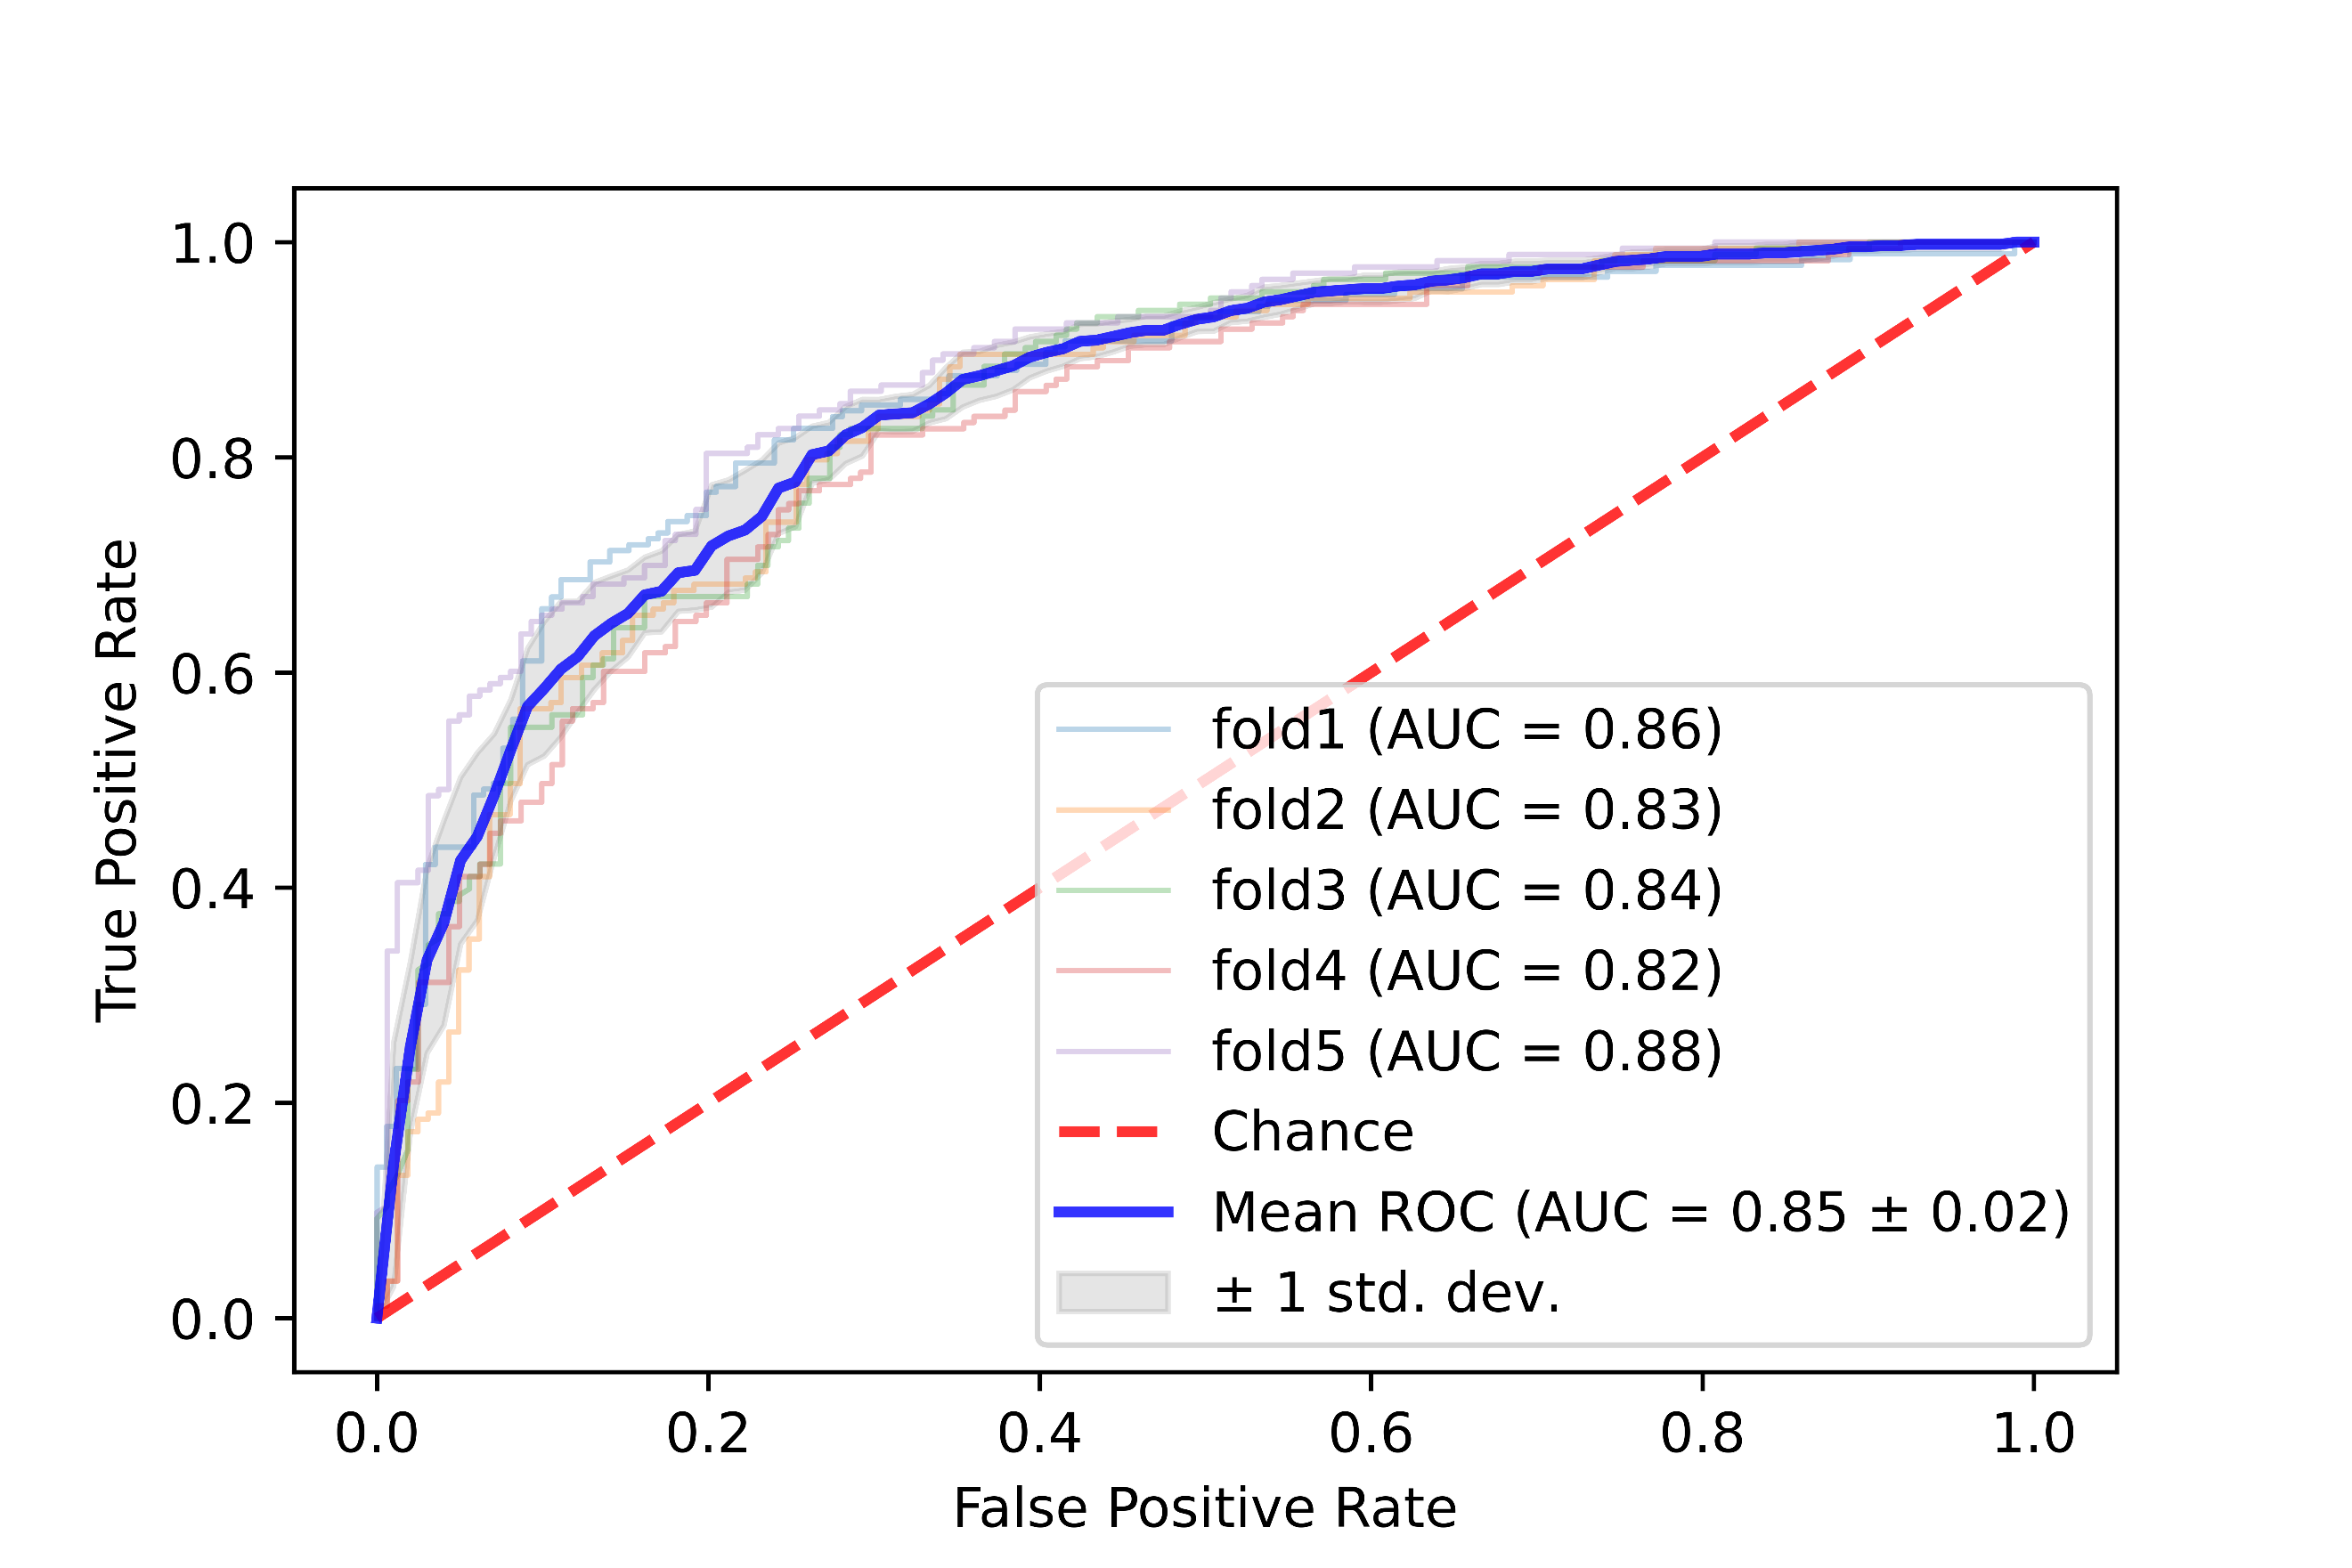
\includegraphics[width=\textwidth,keepaspectratio]{images/Supplement4/image28.png}
		\caption{ROC curve.}
	\end{subfigure}
	\hfill
	\begin{subfigure}[b]{0.49\textwidth}
		\centering
		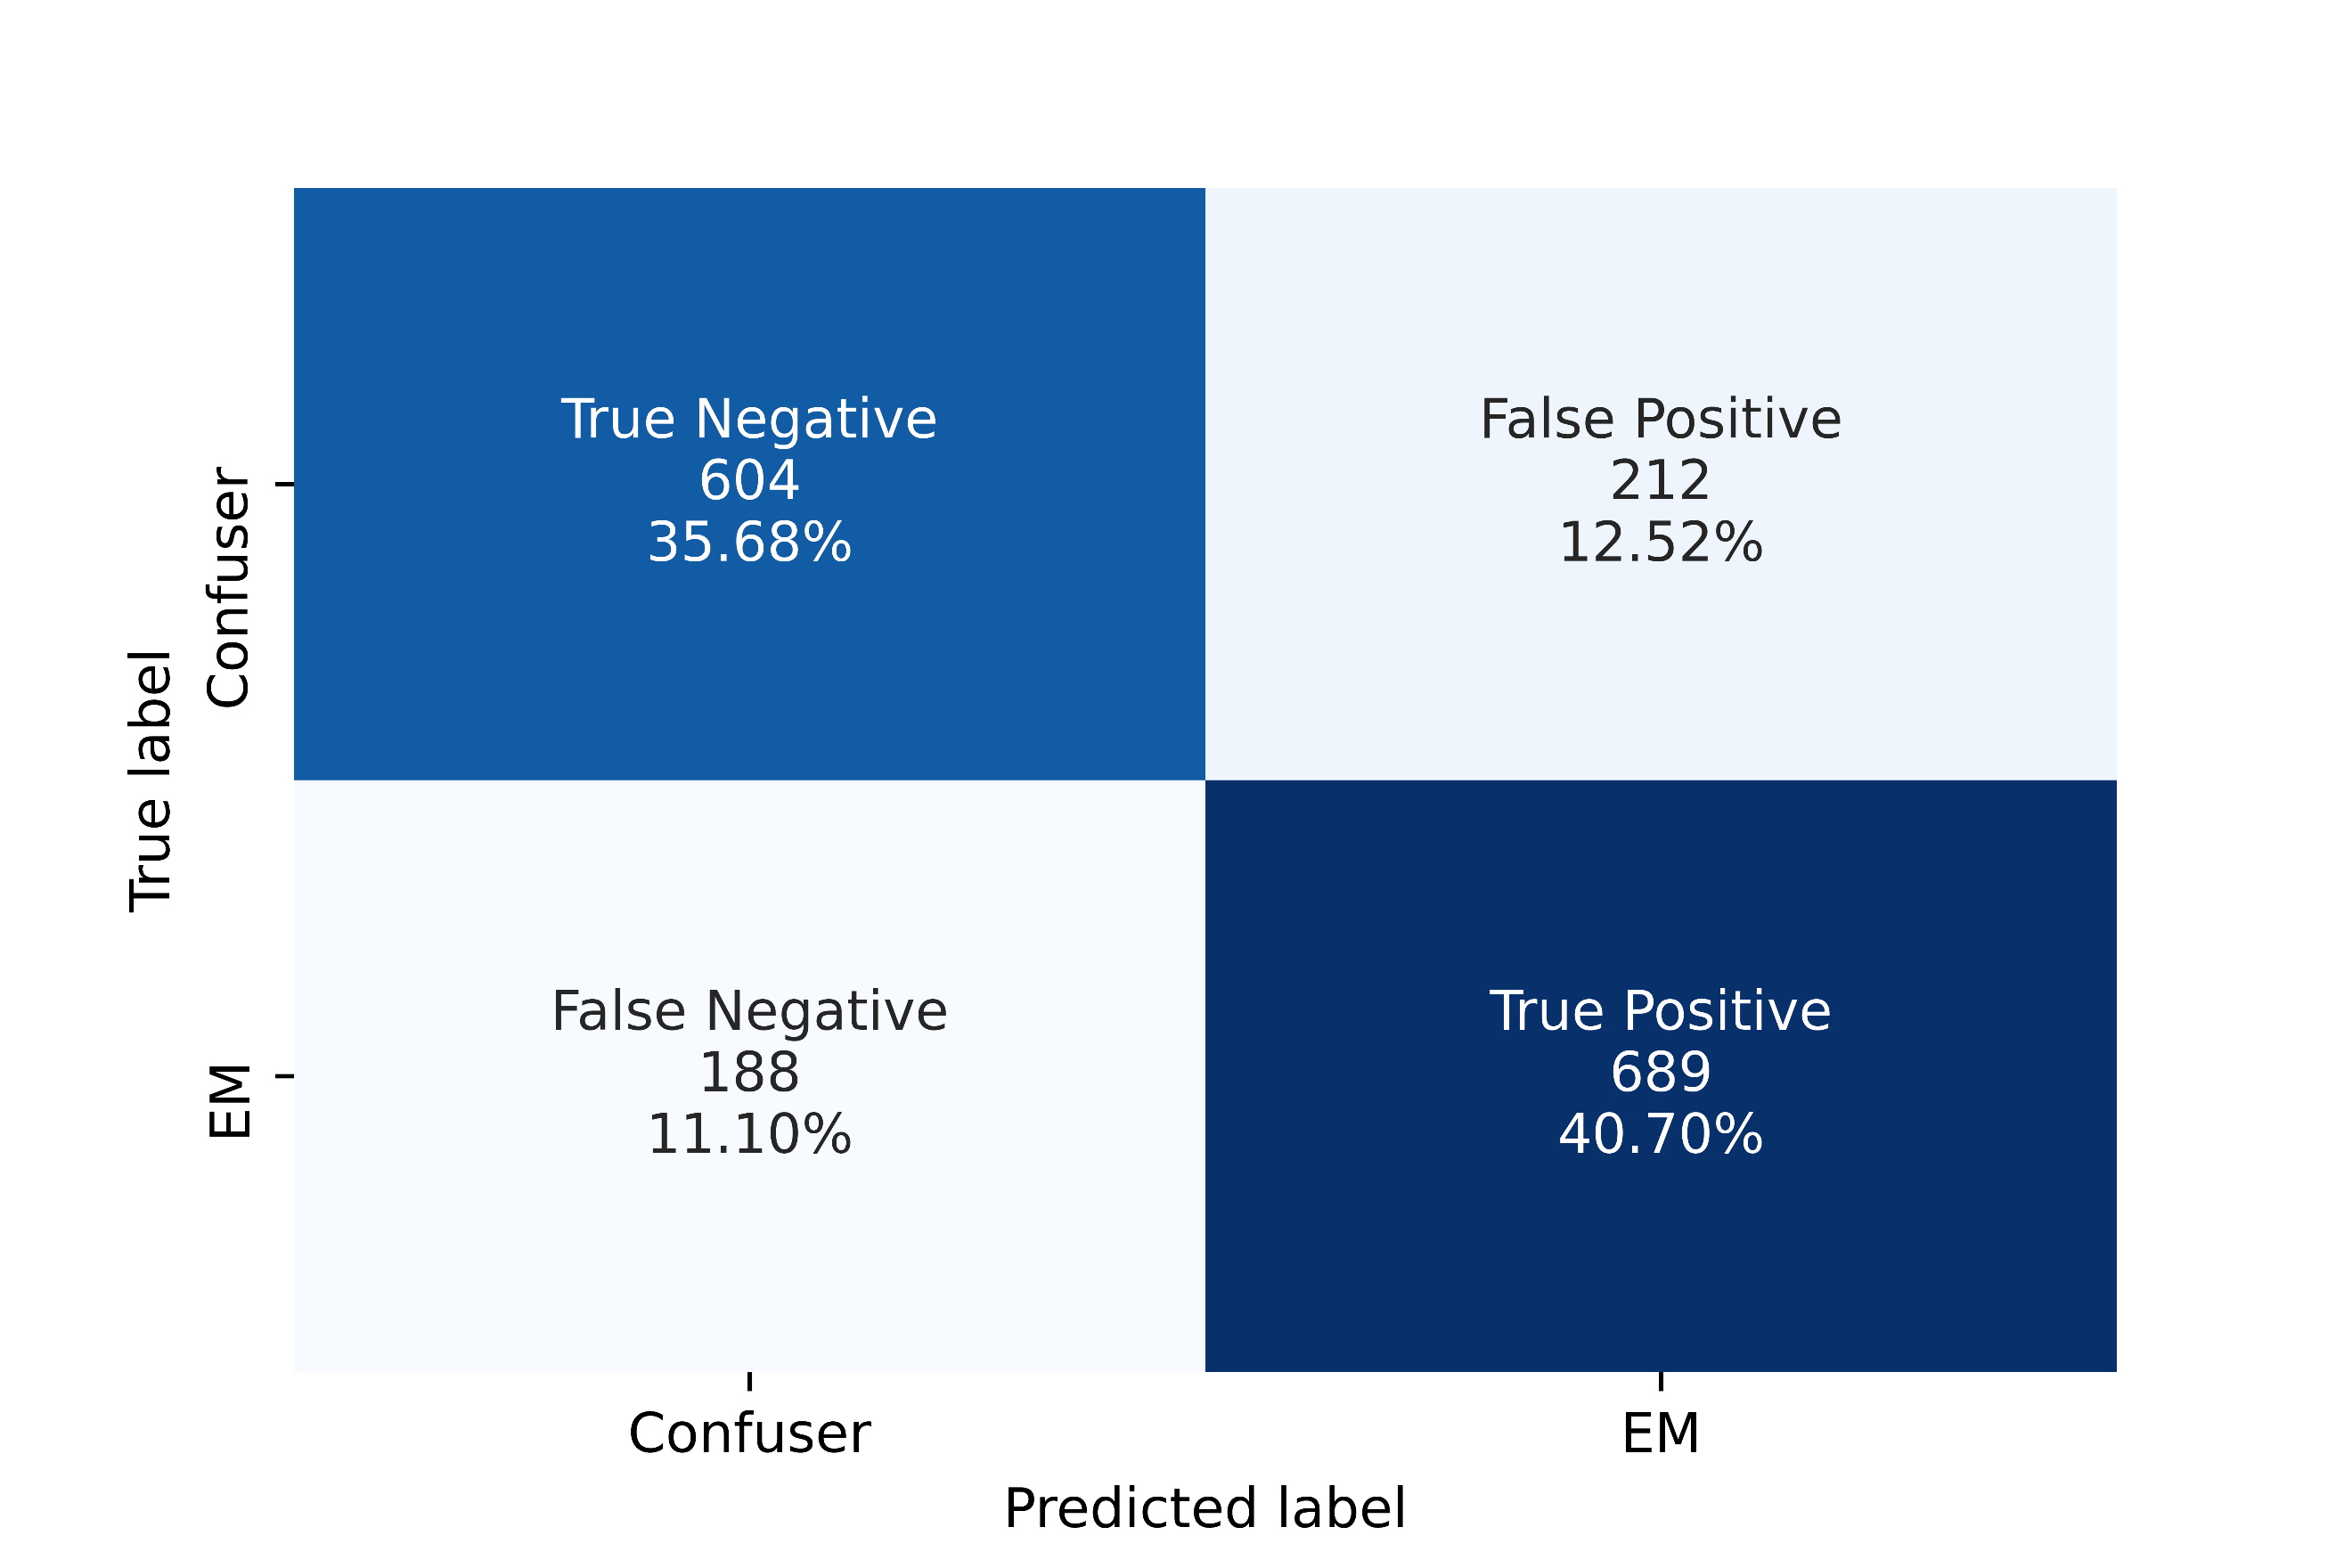
\includegraphics[width=\textwidth,keepaspectratio]{images/Supplement4/image34.png}
		\caption{Confusion matrix.}
	\end{subfigure}
	\caption{Five-fold cross-validation ROC curve and confusion matrix of ResNet50-NTL model.}
\end{figure}

%%%%%%%%%%%%%%Break%%%%%%%%%%%%%%%%%%%%%%
\vfill\clearpage
\subsection{ResNet50-HAM-FFT}

\begin{table}[h!]
	\centering
	\caption{Five-fold cross-validation performance metrics of ResNet50-HAM-FFT model.}
	\resizebox{\textwidth}{!}{%
		\begin{tabular}{llllllllllll}
			\toprule
			& \multicolumn{11}{c}{\textbf{Metric}}    \\ \cmidrule(lr){2-12} 
			\multicolumn{1}{l}{\textbf{Fold}} & \rotatebox{45}{Accuracy} 
			& \rotatebox{45}{Sensitivity} & \rotatebox{45}{Specificity} 
			& \rotatebox{45}{Precision} & \rotatebox{45}{NPV} & \rotatebox{45}{MCC} 
			& \rotatebox{45}{Kappa} 
			& \rotatebox{45}{LR$+$} & \rotatebox{45}{LR$-$} & \rotatebox{45}{F1-Score} 
			& \rotatebox{45}{AUC}  \\ \midrule
			fold1          & 74.72 & 74.05 & 75.44 & 76.54 & 72.88 & 0.4946 & 0.4943 & 3.0151 & 0.3439 & 0.7527 & 0.8255 \\
			fold2          & 71.94 & 76.88 & 66.67 & 71.12 & 72.97 & 0.4382 & 0.4367 & 2.3064 & 0.3468 & 0.7389 & 0.7927 \\
			fold3          & 70.66 & 76.88 & 63.98 & 69.63 & 72.03 & 0.4126 & 0.4101 & 2.134  & 0.3614 & 0.7308 & 0.7596 \\
			fold4          & 70.36 & 74.57 & 65.84 & 70.11 & 70.67 & 0.4059 & 0.405  & 2.1828 & 0.3863 & 0.7227 & 0.7861 \\
			fold5          & 73.65 & 76.88 & 70.19 & 73.48 & 73.86 & 0.472  & 0.4715 & 2.5786 & 0.3294 & 0.7514 & 0.8254 \\\cmidrule(lr){1-12}
			average        & 72.27 & 75.85 & 68.42 & 72.18 & 72.48 & 0.4447 & 0.4435 & 2.4434 & 0.3536 & 0.7393 & 0.7979 \\
			std. deviation & 1.69  & 1.27  & 4.05  & 2.55  & 1.08  & 0.0341 & 0.0347 & 0.3248 & 0.0193 & 0.0116 & 0.0251\\
			\bottomrule
		\end{tabular}%
	}
\end{table}


\begin{figure}[h!]
	\centering
	\begin{subfigure}[b]{0.49\textwidth}
		\centering
		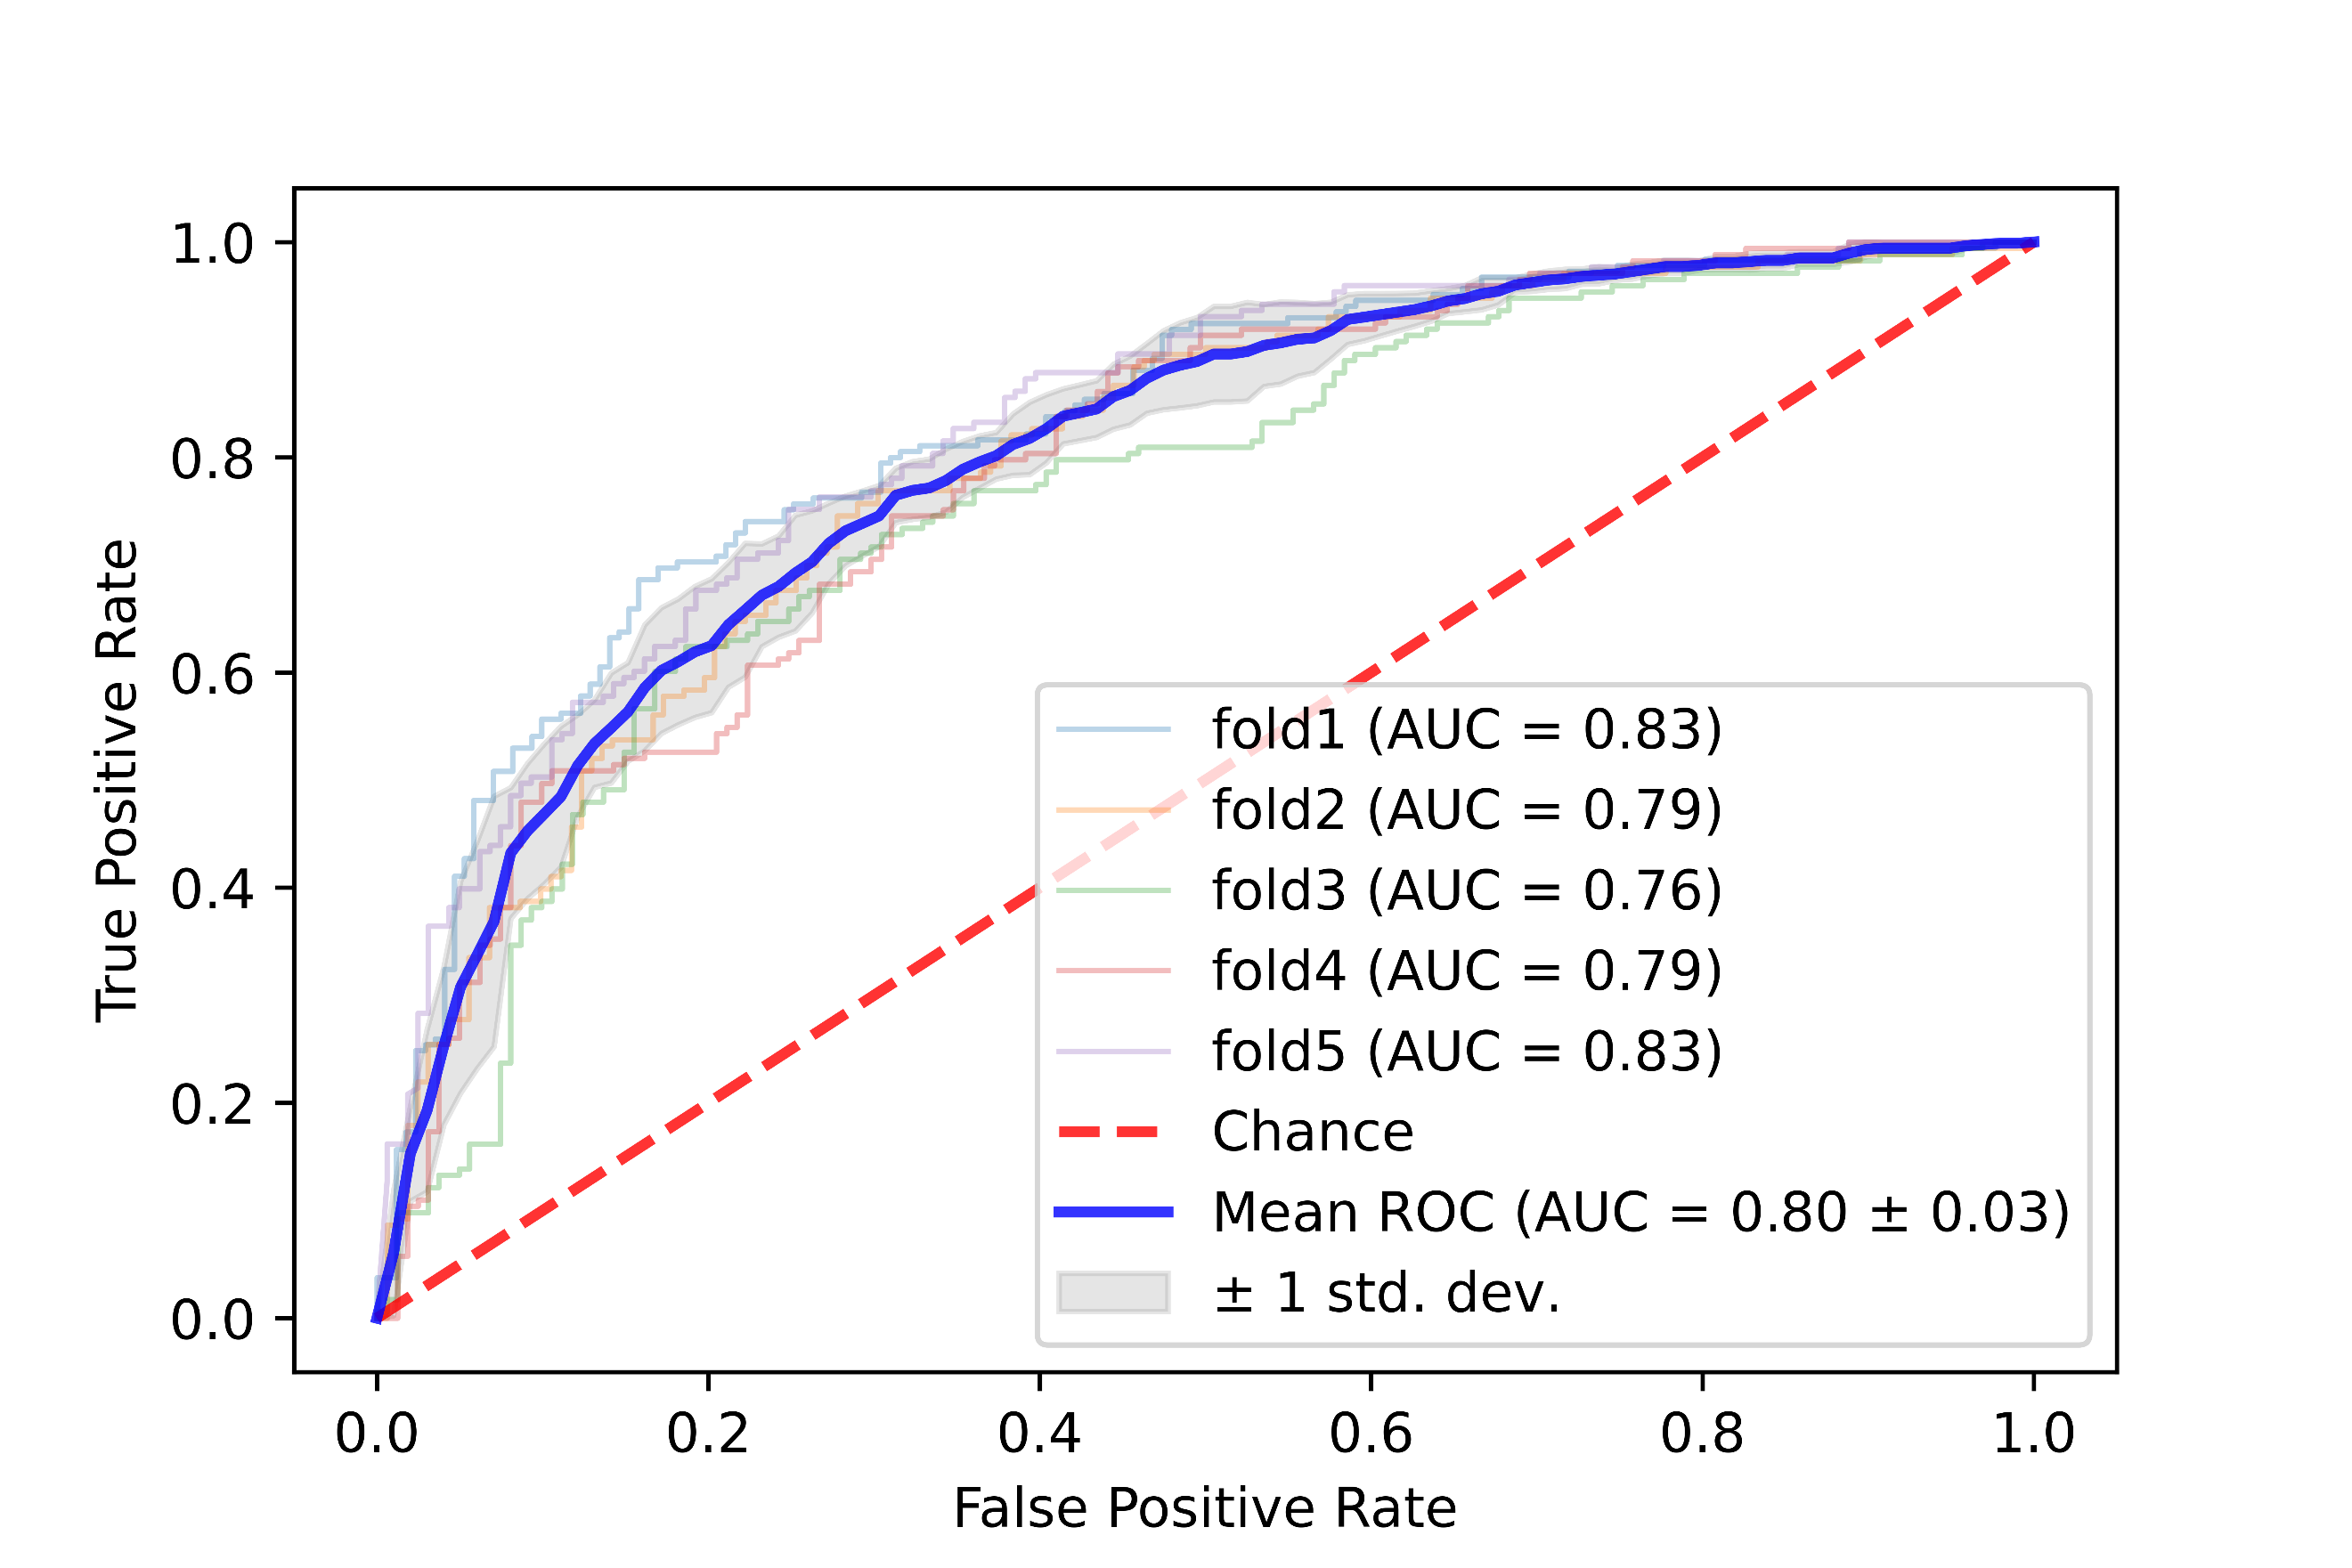
\includegraphics[width=\textwidth,keepaspectratio]{images/Supplement4/image35.png}
		\caption{ROC curve.}
	\end{subfigure}
	\hfill
	\begin{subfigure}[b]{0.49\textwidth}
		\centering
		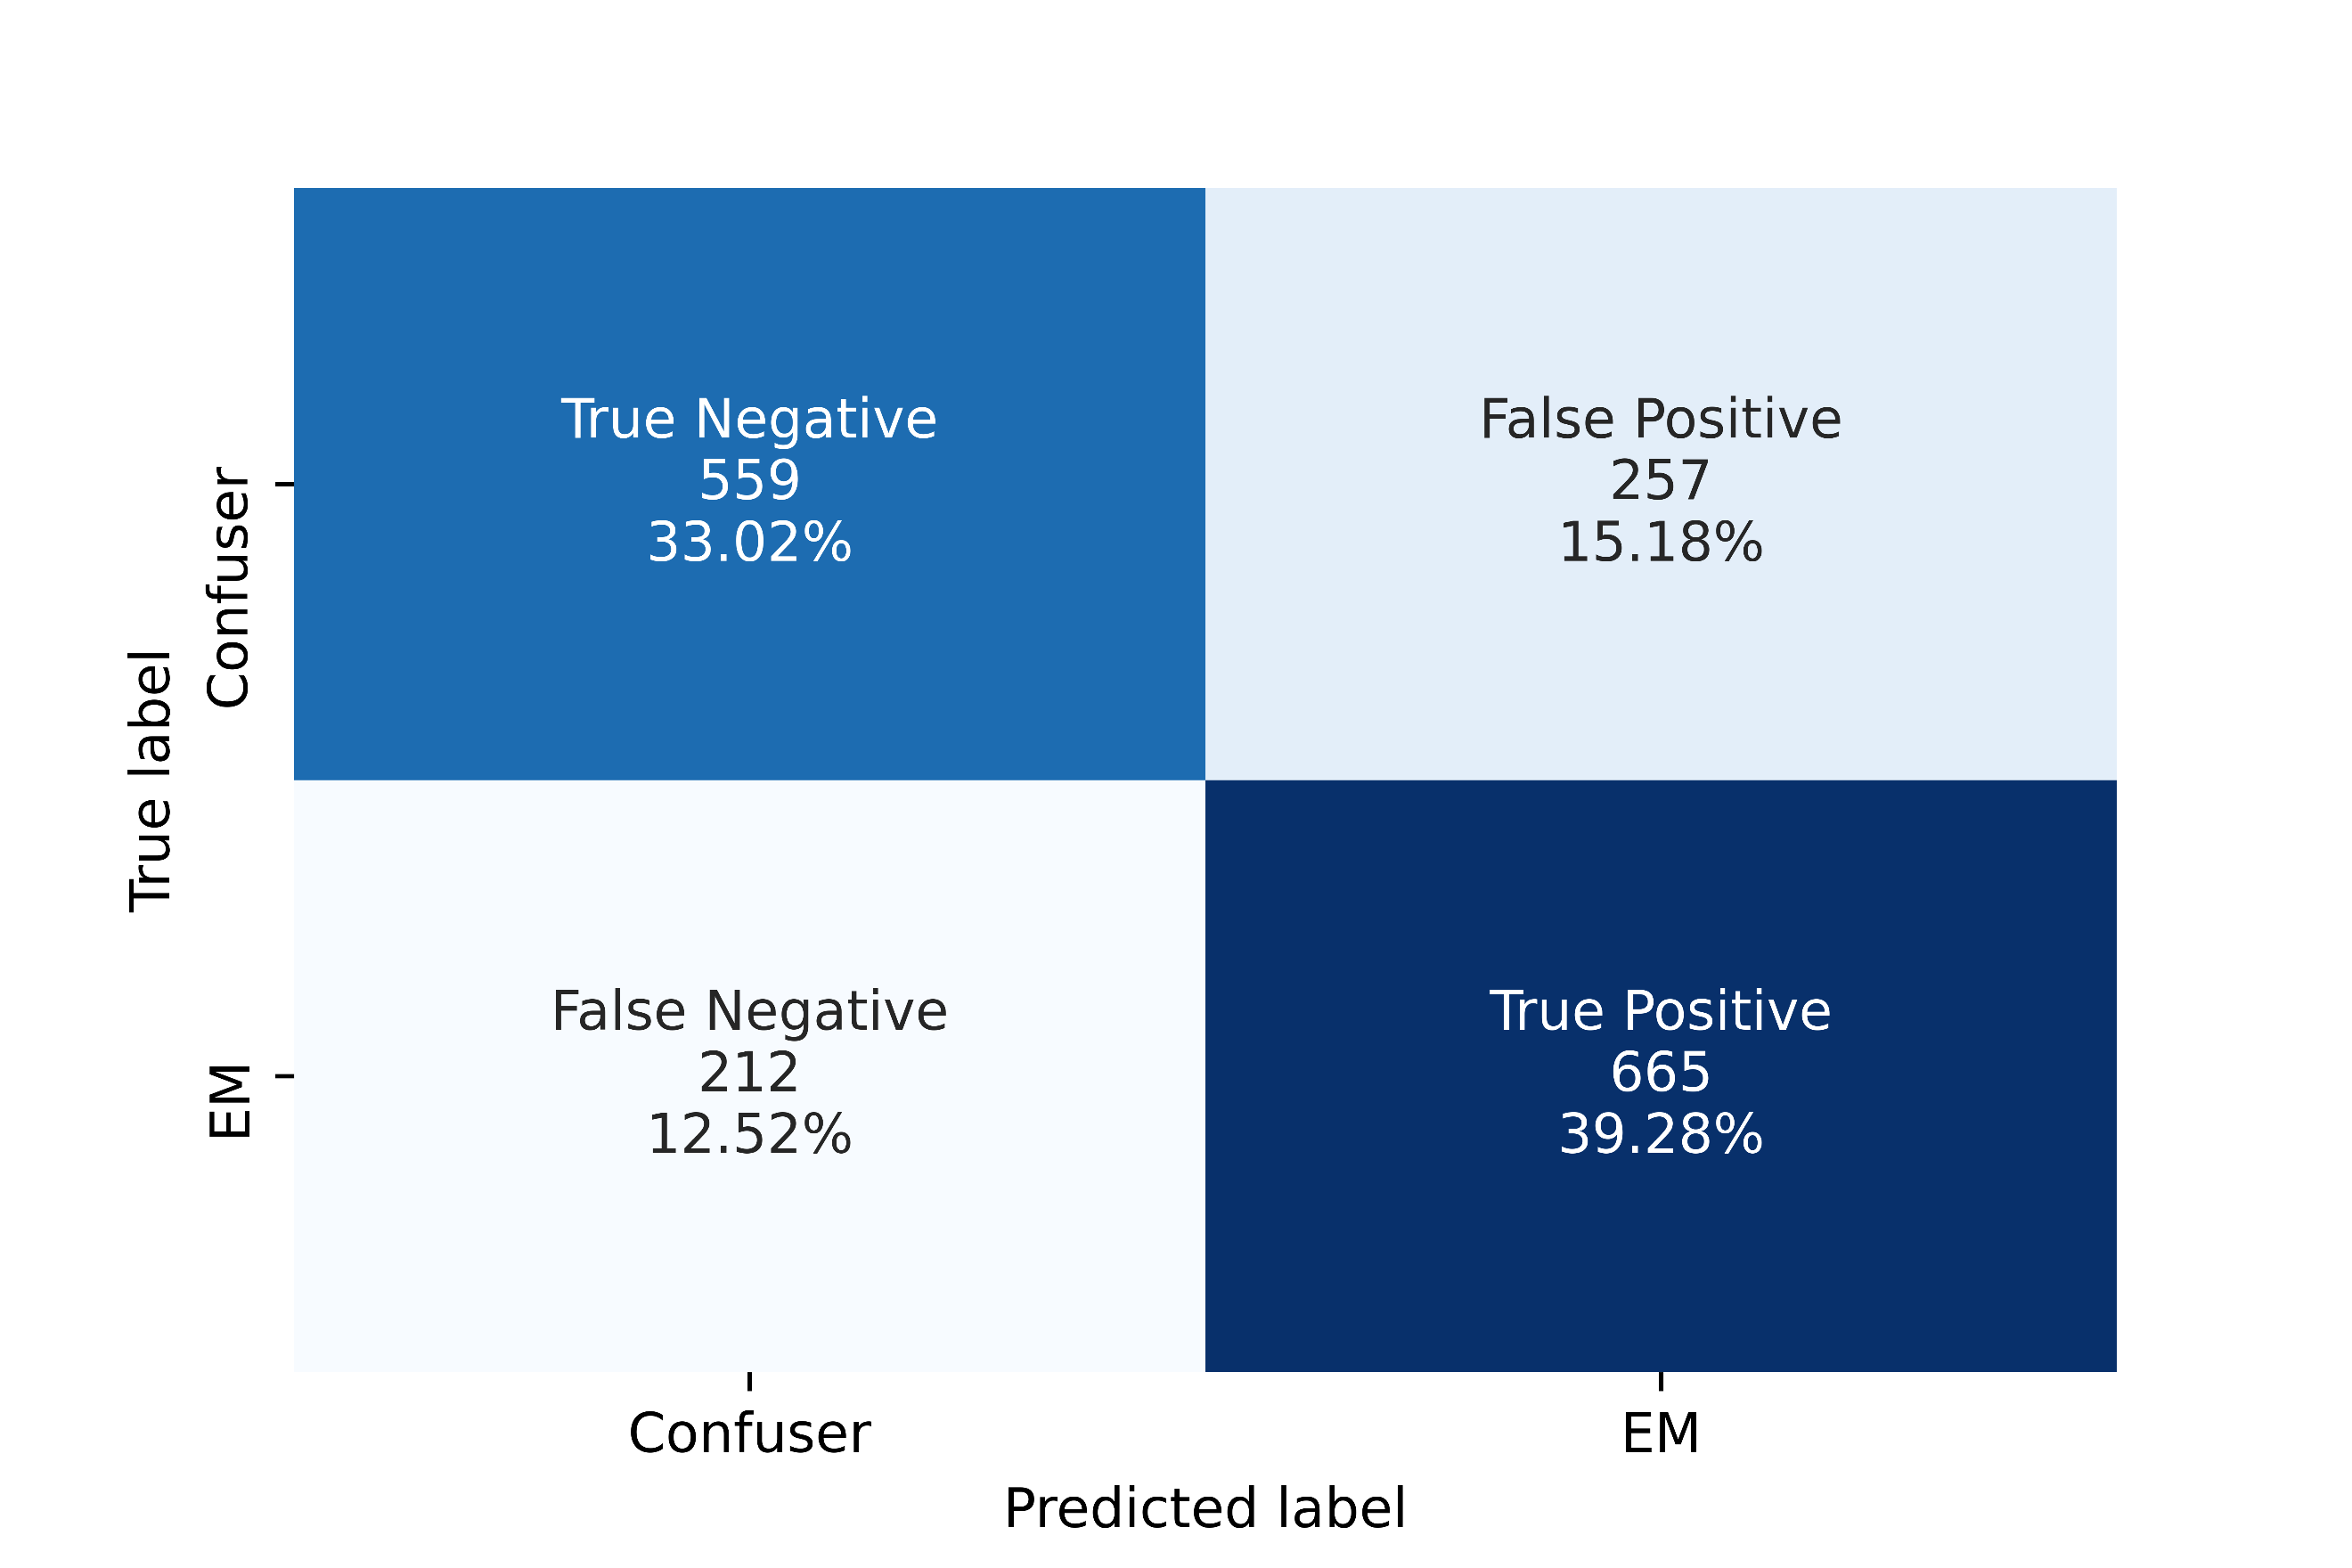
\includegraphics[width=\textwidth,keepaspectratio]{images/Supplement4/image41.png}
		\caption{Confusion matrix.}
	\end{subfigure}
	\caption{Five-fold cross-validation ROC curve and confusion matrix of ResNet50-HAM-FFT model.}
\end{figure}

%%%%%%%%%%%%%%Break%%%%%%%%%%%%%%%%%%%%%%
\vfill\clearpage
\subsection{ResNet50-IMG-WFT}

\begin{table}[h!]
	\centering
	\caption{Five-fold cross-validation performance metrics of ResNet50-IMG-WFT model.}
	\resizebox{\textwidth}{!}{%
		\begin{tabular}{llllllllllll}
			\toprule
			& \multicolumn{11}{c}{\textbf{Metric}}    \\ \cmidrule(lr){2-12} 
			\multicolumn{1}{l}{\textbf{Fold}} & \rotatebox{45}{Accuracy} 
			& \rotatebox{45}{Sensitivity} & \rotatebox{45}{Specificity} 
			& \rotatebox{45}{Precision} & \rotatebox{45}{NPV} & \rotatebox{45}{MCC} 
			& \rotatebox{45}{Kappa} 
			& \rotatebox{45}{LR$+$} & \rotatebox{45}{LR$-$} & \rotatebox{45}{F1-Score} 
			& \rotatebox{45}{AUC}  \\ \midrule
			fold1          & 76.97 & 83.24 & 70.18 & 75.12 & 79.47 & 0.54   & 0.5366 & 2.7911 & 0.2388 & 0.7897 & 0.8379 \\
			fold2          & 78.81 & 79.77 & 77.78 & 79.31 & 78.26 & 0.5756 & 0.5756 & 3.5896 & 0.2601 & 0.7954 & 0.8663 \\
			fold3          & 79.34 & 86.71 & 71.43 & 76.53 & 83.33 & 0.5899 & 0.5842 & 3.0347 & 0.1861 & 0.813  & 0.8667 \\
			fold4          & 78.14 & 83.82 & 72.05 & 76.32 & 80.56 & 0.5637 & 0.5607 & 2.9987 & 0.2246 & 0.7989 & 0.8744 \\
			fold5          & 81.44 & 79.19 & 83.85 & 84.05 & 78.95 & 0.6302 & 0.6291 & 4.9037 & 0.2482 & 0.8155 & 0.8875 \\\cmidrule(lr){1-12} 
			average        & 78.94 & 82.55 & 75.06 & 78.27 & 80.11 & 0.5799 & 0.5772 & 3.4636 & 0.2316 & 0.8025 & 0.8666 \\
			std. deviation & 1.48  & 2.77  & 5.11  & 3.2   & 1.77  & 0.03   & 0.0305 & 0.7671 & 0.0255 & 0.0101 & 0.0163\\
			\bottomrule
		\end{tabular}%
	}
\end{table}


\begin{figure}[h!]
	\centering
	\begin{subfigure}[b]{0.49\textwidth}
		\centering
		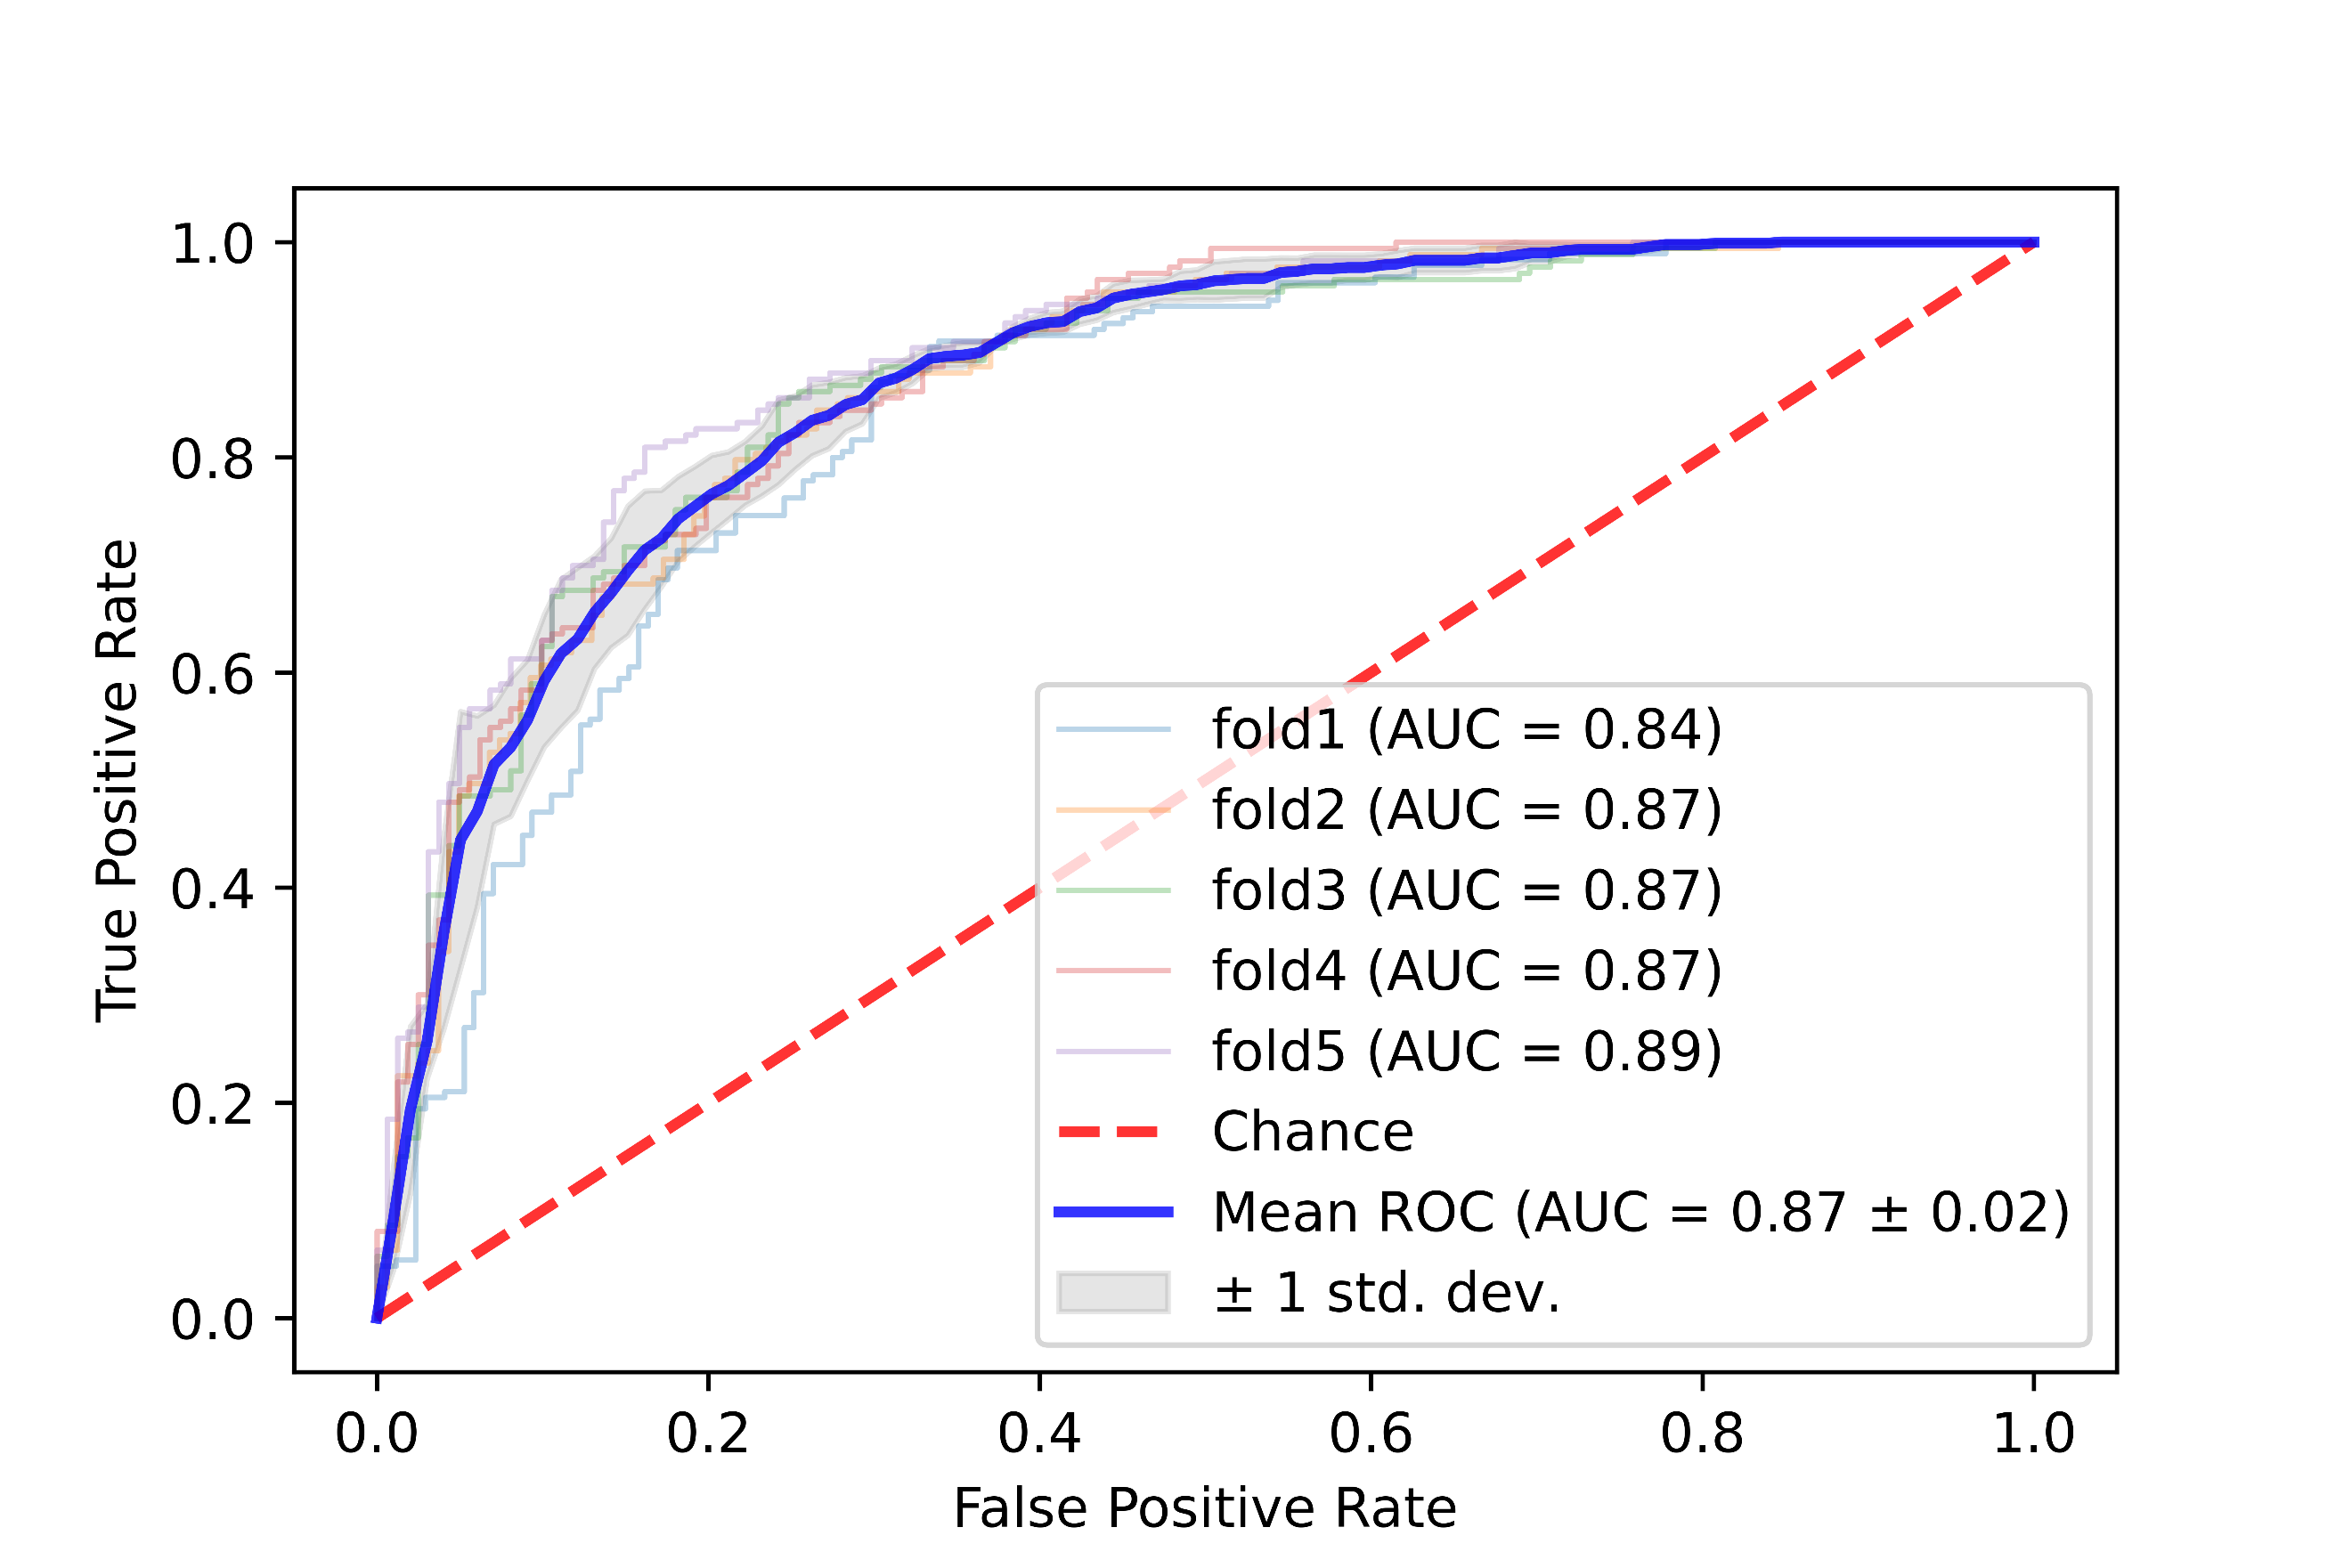
\includegraphics[width=\textwidth,keepaspectratio]{images/Supplement4/image42.png}
		\caption{ROC curve.}
	\end{subfigure}
	\hfill
	\begin{subfigure}[b]{0.49\textwidth}
		\centering
		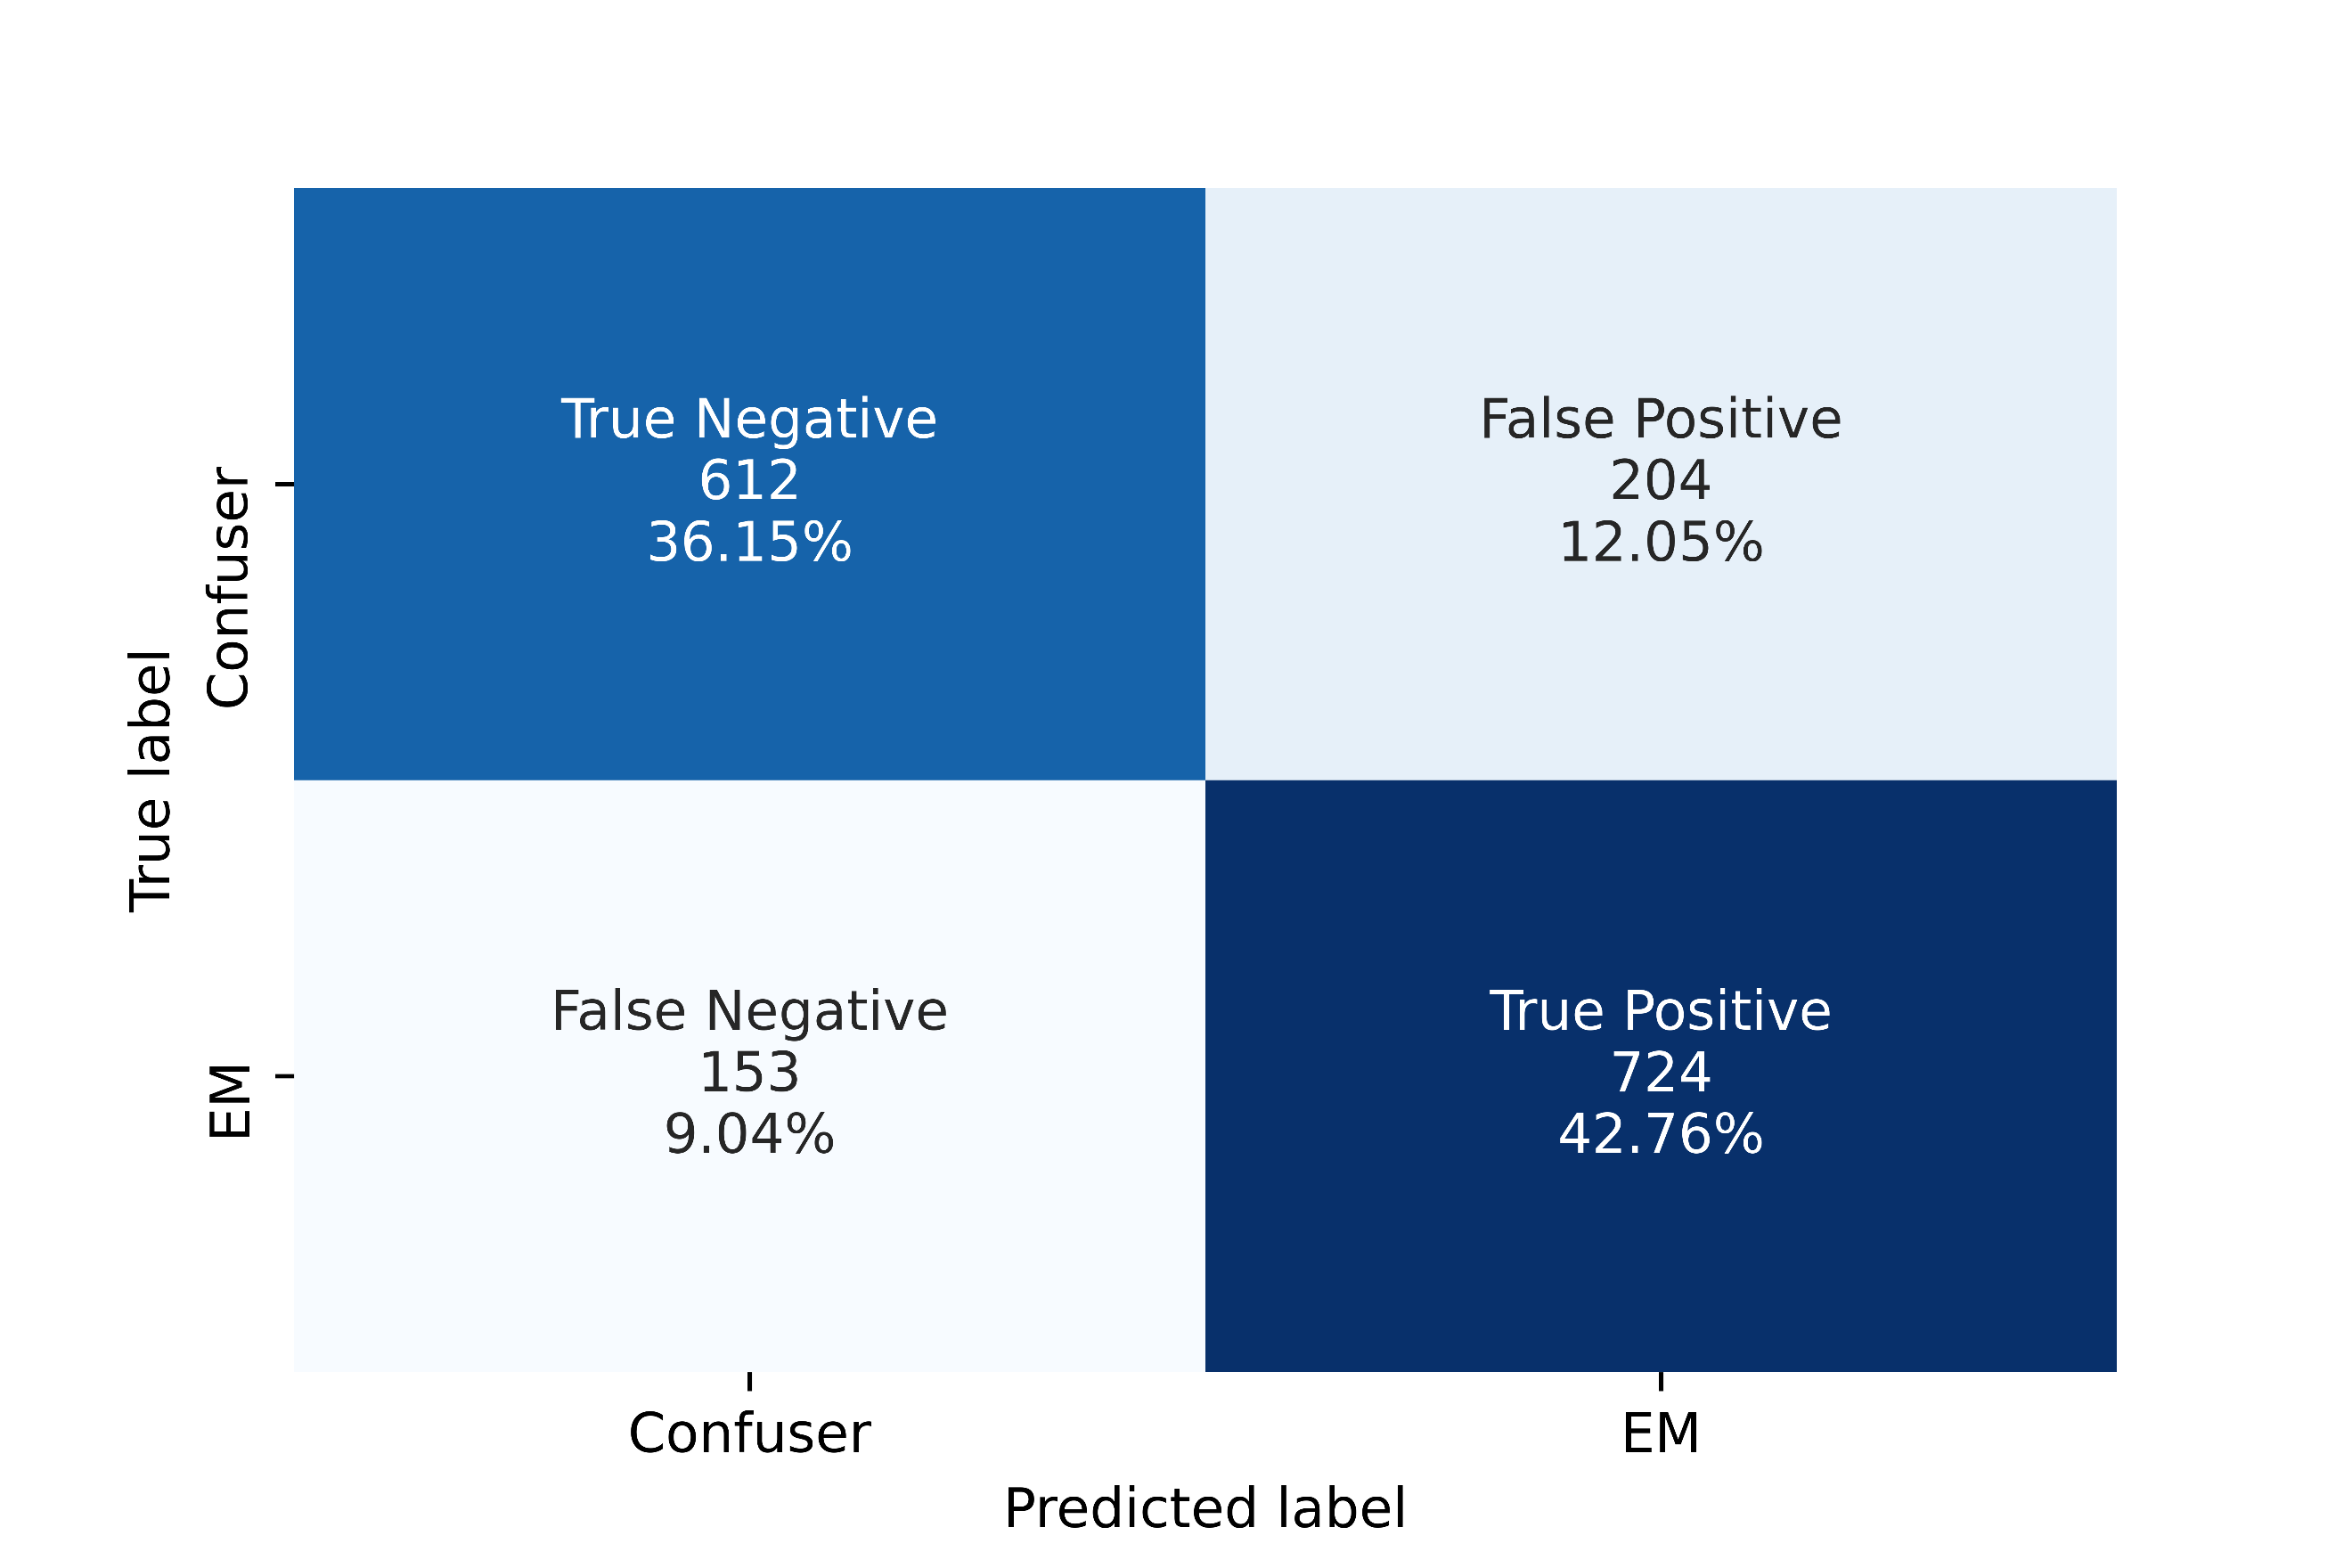
\includegraphics[width=\textwidth,keepaspectratio]{images/Supplement4/image48.png}
		\caption{Confusion matrix.}
	\end{subfigure}
	\caption{Five-fold cross-validation ROC curve and confusion matrix of ResNet50-IMG-WFT model.}
\end{figure}

%%%%%%%%%%%%%%Break%%%%%%%%%%%%%%%%%%%%%%
\vfill\clearpage
\subsection{ResNet50-IMG-FFT}

\begin{table}[h!]
	\centering
	\caption{Five-fold cross-validation performance metrics of ResNet50-IMG-FFT model.}
	\resizebox{\textwidth}{!}{%
		\begin{tabular}{llllllllllll}
			\toprule
			& \multicolumn{11}{c}{\textbf{Metric}}    \\ \cmidrule(lr){2-12} 
			\multicolumn{1}{l}{\textbf{Fold}} & \rotatebox{45}{Accuracy} 
			& \rotatebox{45}{Sensitivity} & \rotatebox{45}{Specificity} 
			& \rotatebox{45}{Precision} & \rotatebox{45}{NPV} & \rotatebox{45}{MCC} 
			& \rotatebox{45}{Kappa} 
			& \rotatebox{45}{LR$+$} & \rotatebox{45}{LR$-$} & \rotatebox{45}{F1-Score} 
			& \rotatebox{45}{AUC}  \\ \midrule
			fold1          & 82.58 & 87.03 & 77.78 & 80.9  & 84.71 & 0.6521 & 0.6501 & 3.9162 & 0.1668 & 0.8385 & 0.895  \\
			fold2          & 82.09 & 82.08 & 82.1  & 83.04 & 81.1  & 0.6416 & 0.6415 & 4.5852 & 0.2183 & 0.8256 & 0.9051 \\
			fold3          & 80.24 & 88.44 & 71.43 & 76.88 & 85.19 & 0.6096 & 0.6021 & 3.0954 & 0.1618 & 0.8226 & 0.9114 \\
			fold4          & 84.43 & 82.08 & 86.96 & 87.12 & 81.87 & 0.6901 & 0.6889 & 6.2929 & 0.2061 & 0.8452 & 0.9234 \\
			fold5          & 81.74 & 86.71 & 76.4  & 79.79 & 84.25 & 0.6357 & 0.6331 & 3.6736 & 0.174  & 0.831  & 0.9101 \\\cmidrule(lr){1-12}
			average        & 82.22 & 85.27 & 78.93 & 81.55 & 83.42 & 0.6458 & 0.6431 & 4.3127 & 0.1854 & 0.8326 & 0.909  \\
			std. deviation & 1.36  & 2.67  & 5.26  & 3.42  & 1.63  & 0.0262 & 0.028  & 1.0994 & 0.0226 & 0.0083 & 0.0092\\
			\bottomrule
		\end{tabular}%
	}
\end{table}


\begin{figure}[h!]
	\centering
	\begin{subfigure}[b]{0.49\textwidth}
		\centering
		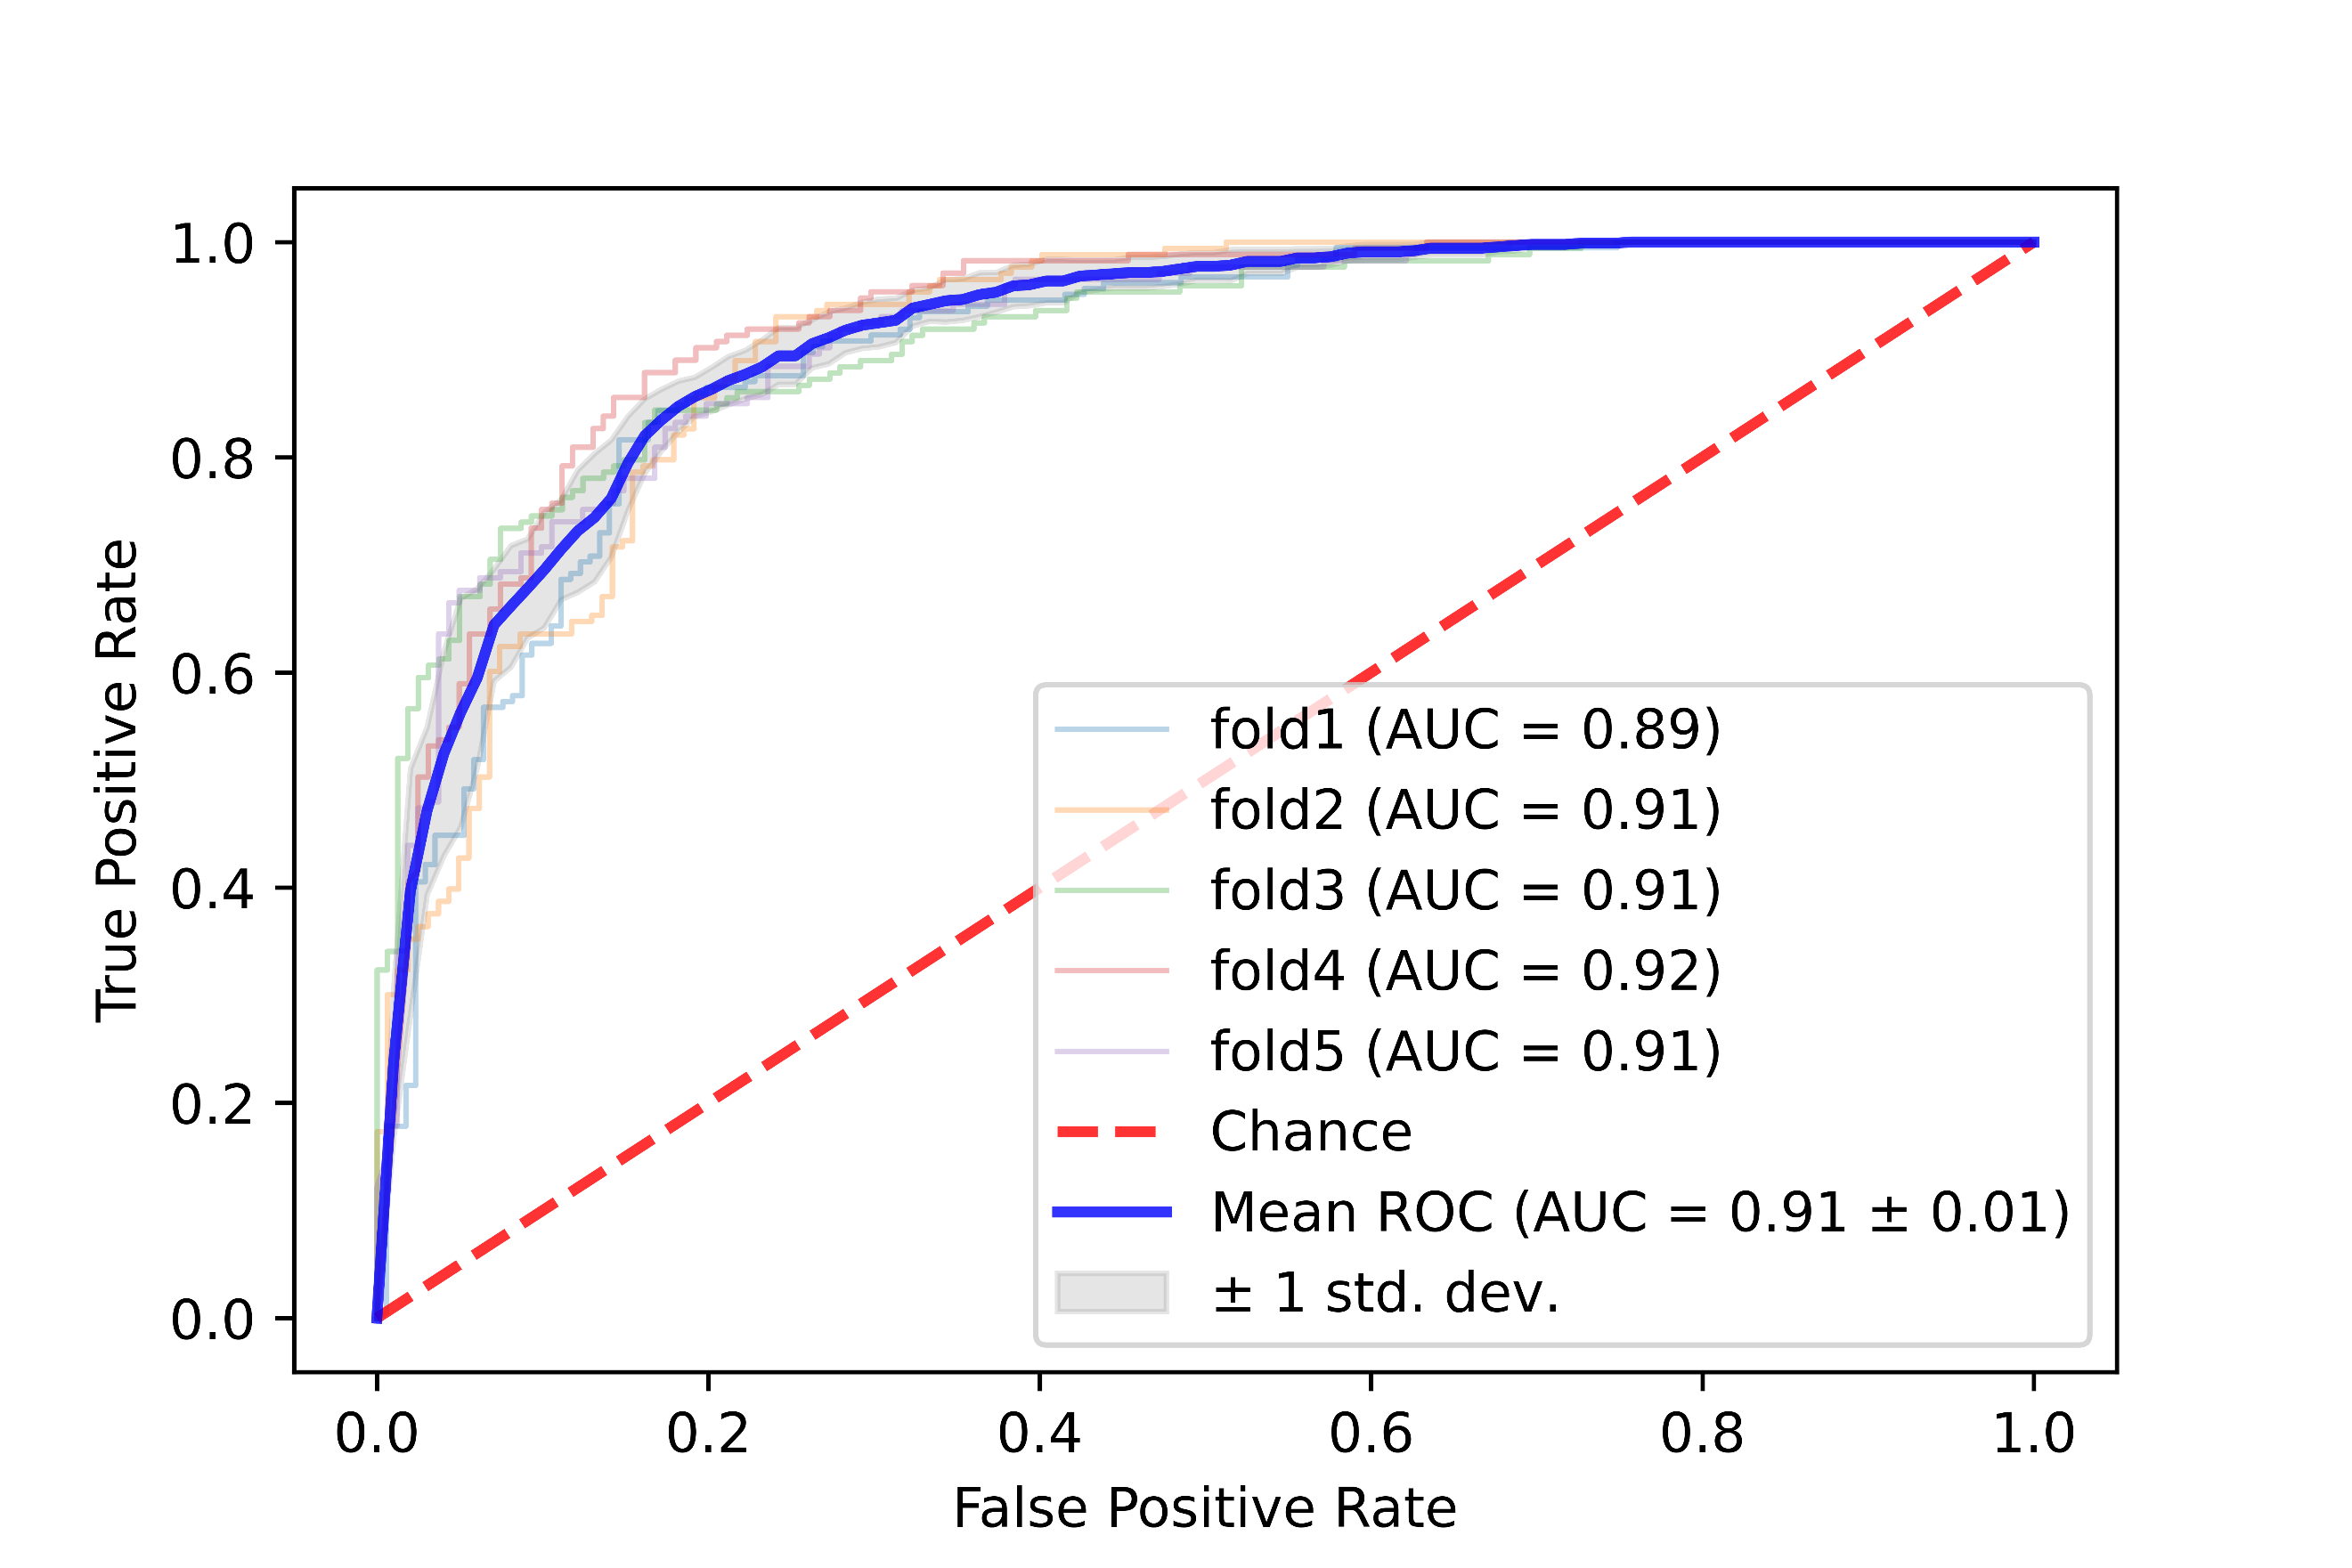
\includegraphics[width=\textwidth,keepaspectratio]{images/Supplement4/image49.png}
		\caption{ROC curve.}
	\end{subfigure}
	\hfill
	\begin{subfigure}[b]{0.49\textwidth}
		\centering
		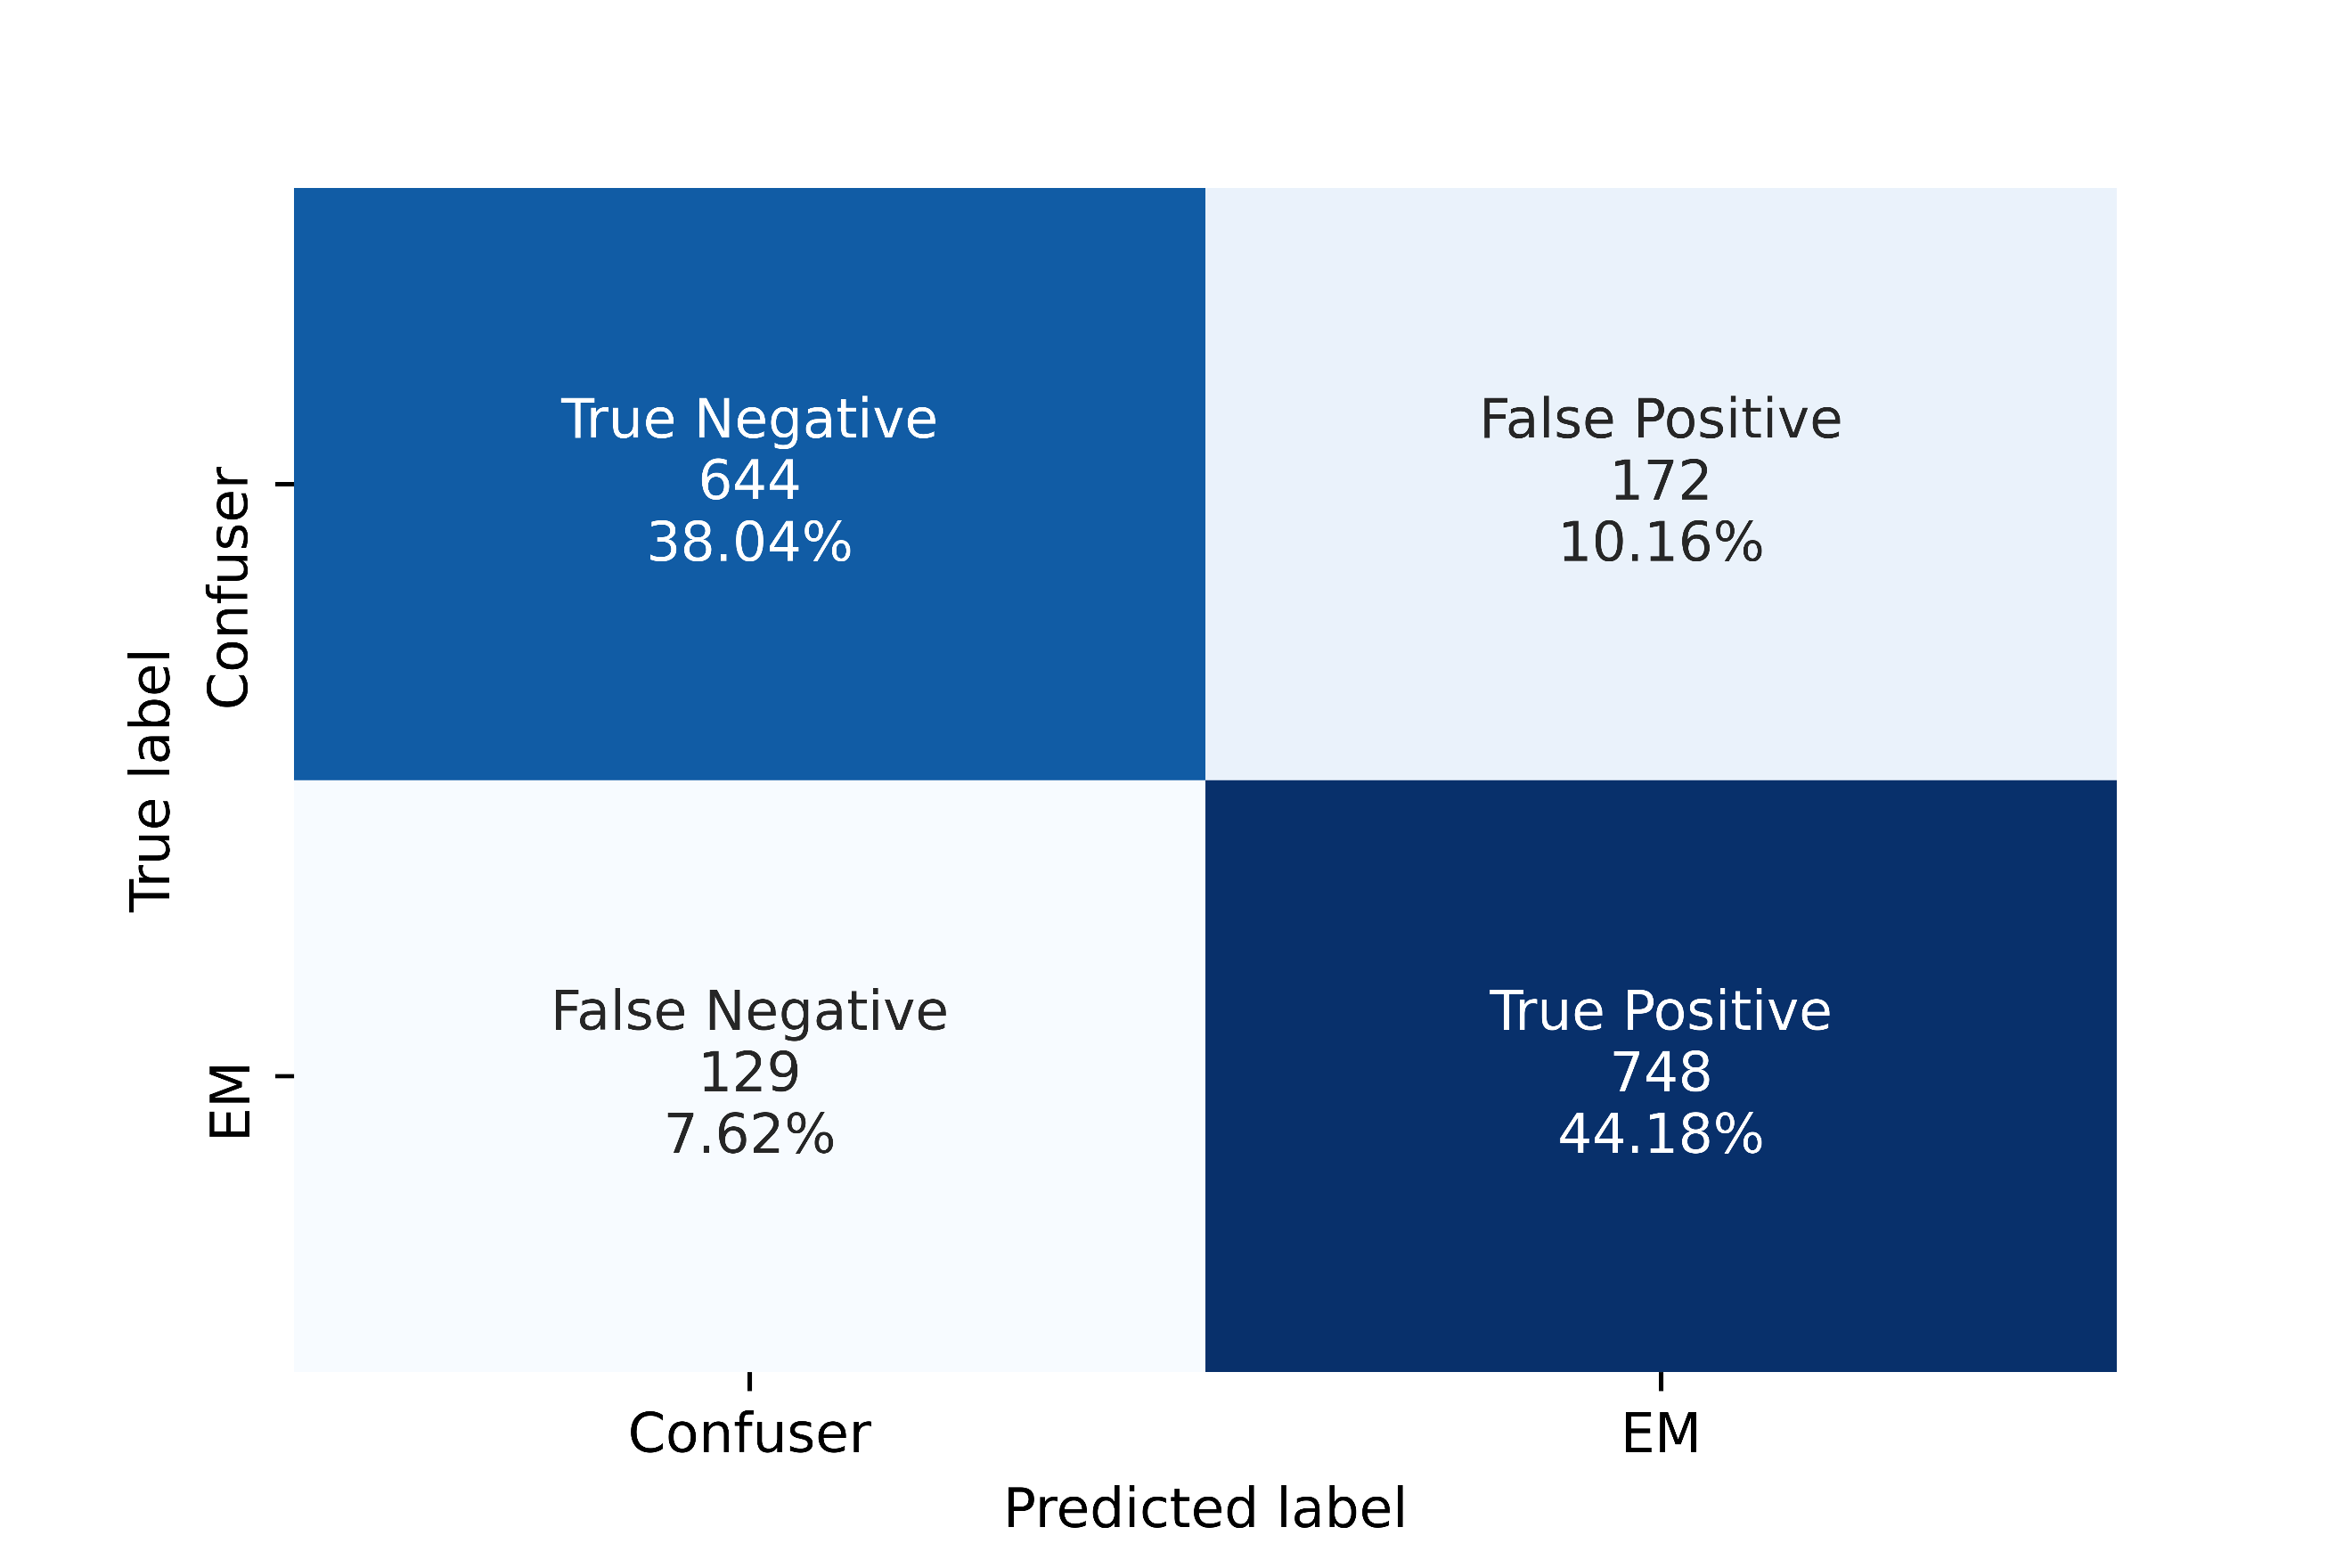
\includegraphics[width=\textwidth,keepaspectratio]{images/Supplement4/image55.png}
		\caption{Confusion matrix.}
	\end{subfigure}
	\caption{Five-fold cross-validation ROC curve and confusion matrix of ResNet50-IMG-FFT model.}
\end{figure}

%%%%%%%%%%%%%%Break%%%%%%%%%%%%%%%%%%%%%%
\vfill\clearpage
\subsection{ResNet50-IMG-FT141}

\begin{table}[h!]
	\centering
	\caption{Five-fold cross-validation performance metrics of ResNet50-IMG-FT141 model.}
	\resizebox{\textwidth}{!}{%
		\begin{tabular}{llllllllllll}
			\toprule
			& \multicolumn{11}{c}{\textbf{Metric}}    \\ \cmidrule(lr){2-12} 
			\multicolumn{1}{l}{\textbf{Fold}} & \rotatebox{45}{Accuracy} 
			& \rotatebox{45}{Sensitivity} & \rotatebox{45}{Specificity} 
			& \rotatebox{45}{Precision} & \rotatebox{45}{NPV} & \rotatebox{45}{MCC} 
			& \rotatebox{45}{Kappa} 
			& \rotatebox{45}{LR$+$} & \rotatebox{45}{LR$-$} & \rotatebox{45}{F1-Score} 
			& \rotatebox{45}{AUC}  \\ \midrule
			fold1          & 81.74 & 85.41 & 77.78 & 80.61 & 83.12 & 0.6346 & 0.6334 & 3.8432 & 0.1876 & 0.8294 & 0.9003 \\
			fold2          & 84.18 & 86.13 & 82.1  & 83.71 & 84.71 & 0.6832 & 0.6829 & 4.8112 & 0.169  & 0.849  & 0.9102 \\
			fold3          & 82.34 & 83.24 & 81.37 & 82.76 & 81.88 & 0.6462 & 0.6462 & 4.4671 & 0.206  & 0.83   & 0.9091 \\
			fold4          & 84.43 & 89.02 & 79.5  & 82.35 & 87.07 & 0.6897 & 0.6873 & 4.343  & 0.1381 & 0.8556 & 0.9246 \\
			fold5          & 83.53 & 82.66 & 84.47 & 85.12 & 81.93 & 0.6709 & 0.6706 & 5.3232 & 0.2053 & 0.8387 & 0.9228 \\\cmidrule(lr){1-12}
			average        & 83.24 & 85.29 & 81.04 & 82.91 & 83.74 & 0.6649 & 0.6641 & 4.5575 & 0.1812 & 0.8405 & 0.9134 \\
			std. deviation & 1.04  & 2.27  & 2.28  & 1.49  & 1.96  & 0.0212 & 0.021  & 0.493  & 0.0255 & 0.0104 & 0.0091\\
			\bottomrule
		\end{tabular}%
	}
\end{table}


\begin{figure}[h!]
	\centering
	\begin{subfigure}[b]{0.49\textwidth}
		\centering
		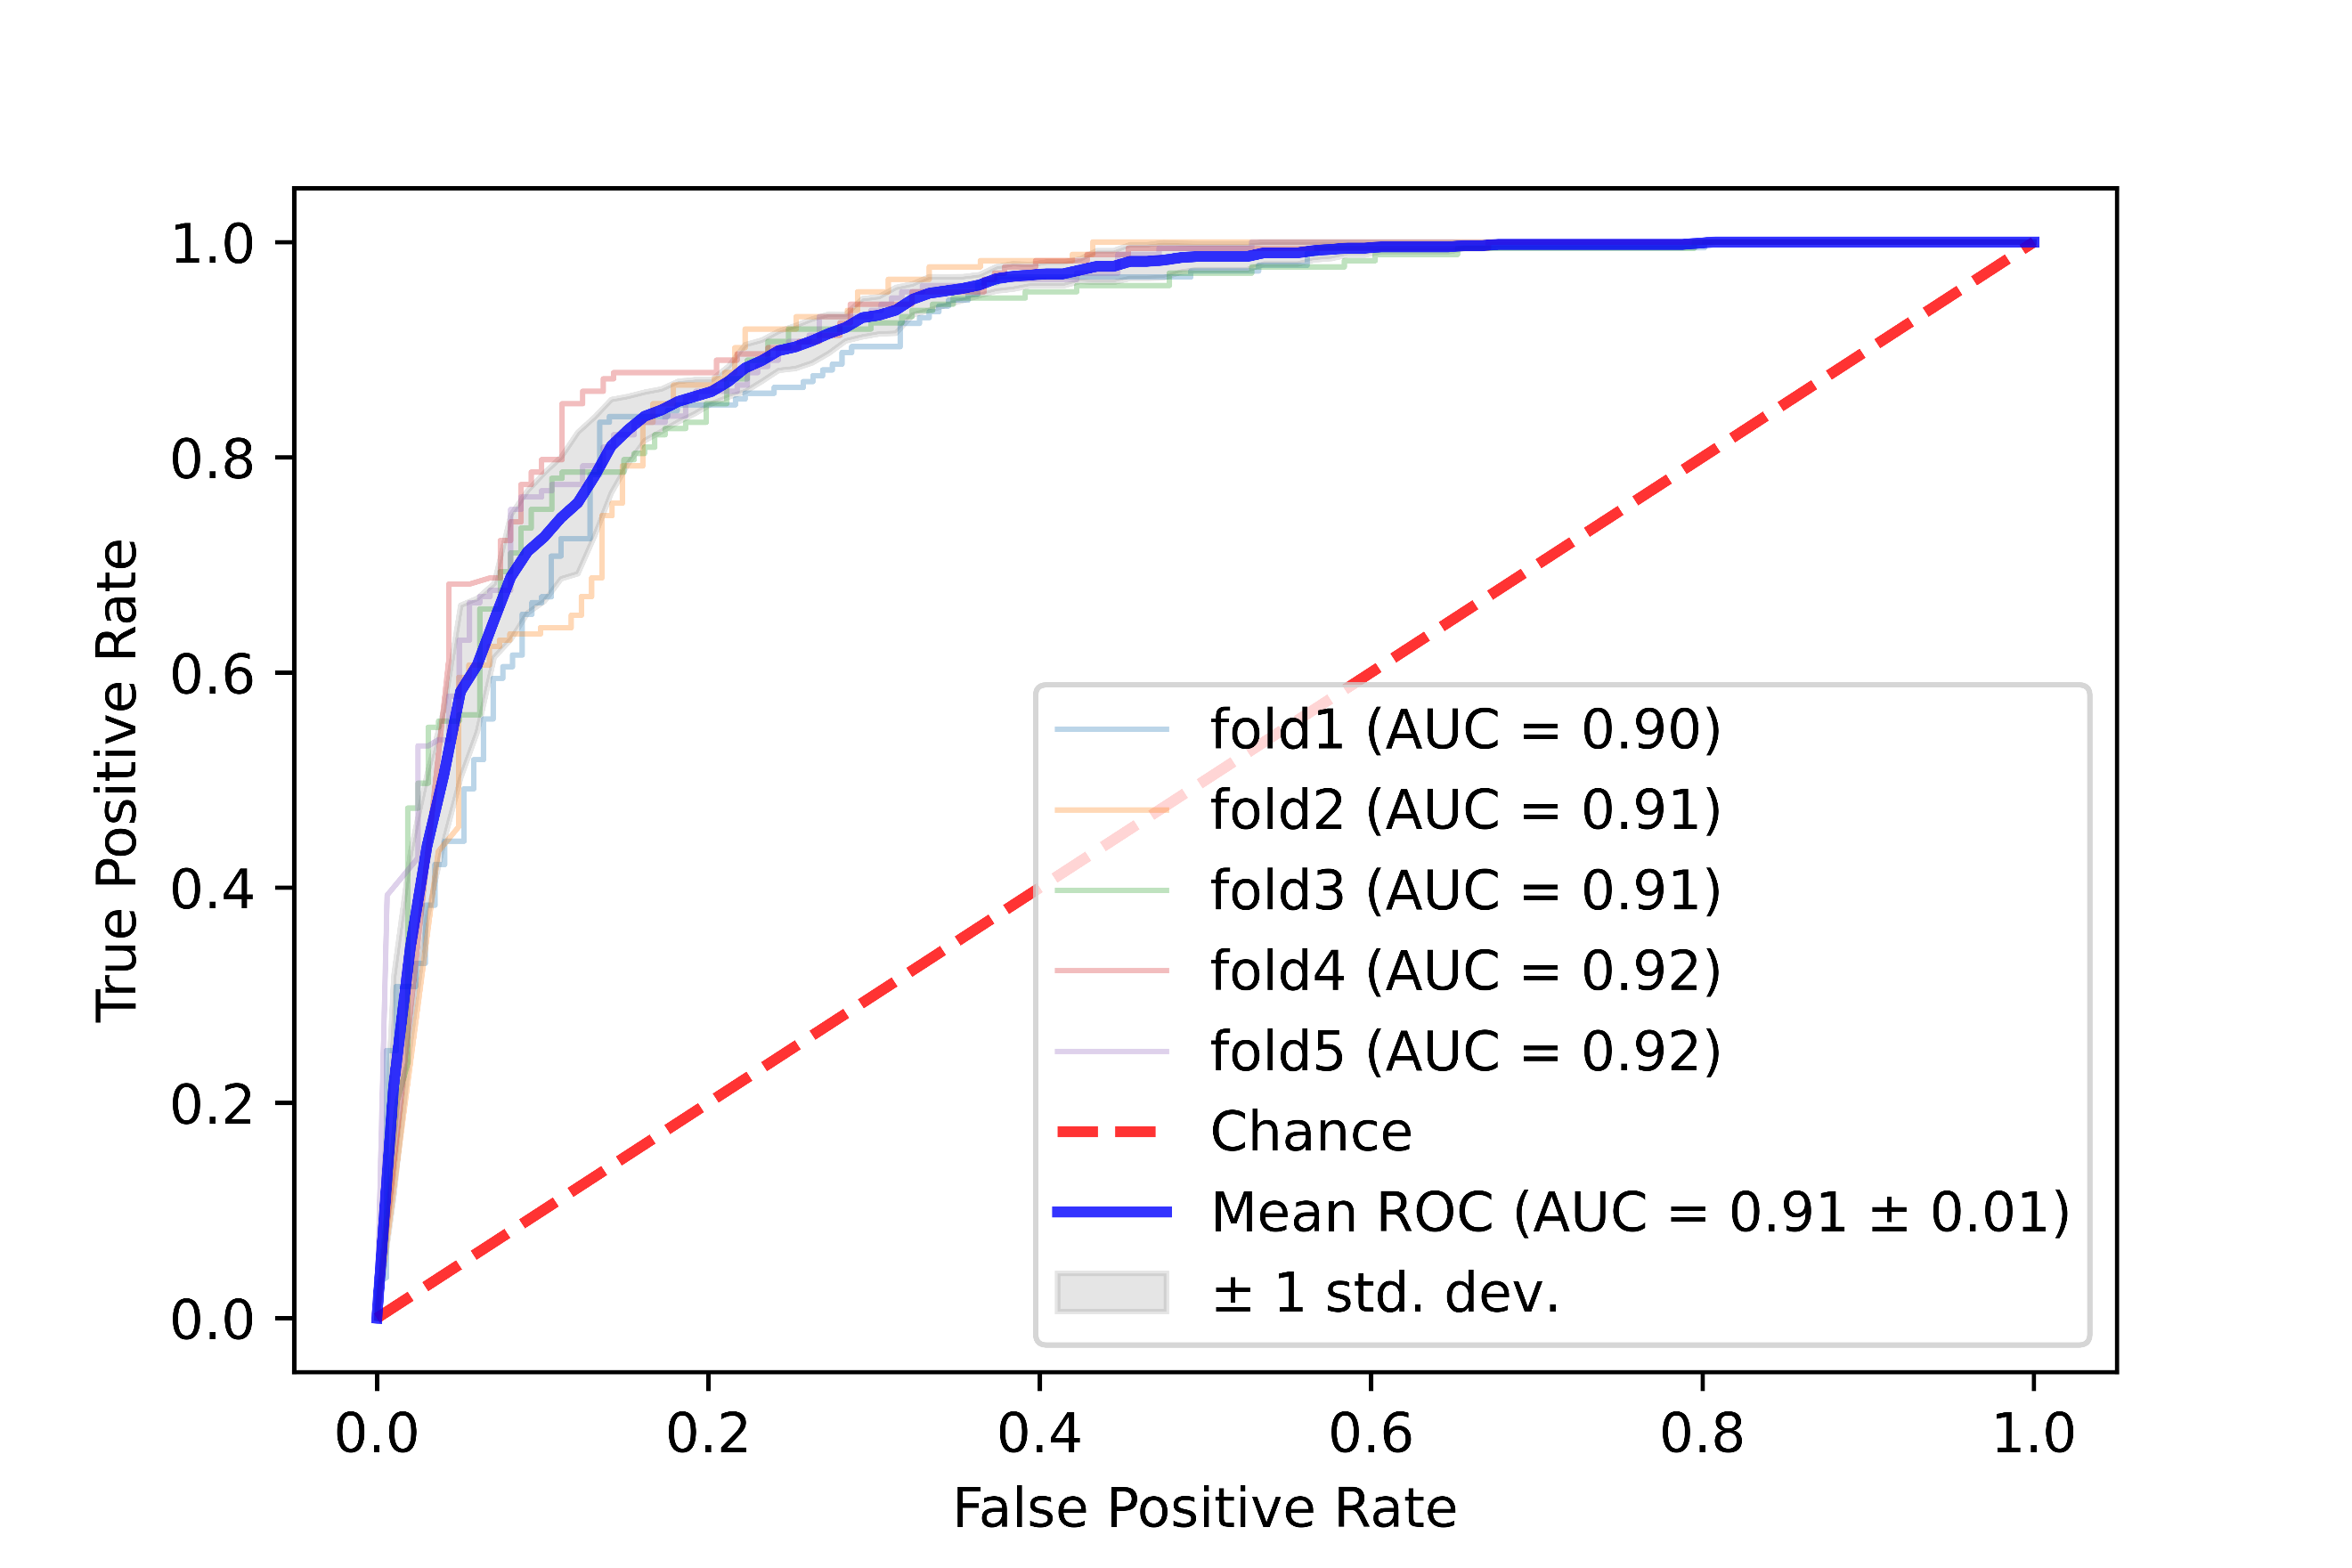
\includegraphics[width=\textwidth,keepaspectratio]{images/Supplement4/image56.png}
		\caption{ROC curve.}
	\end{subfigure}
	\hfill
	\begin{subfigure}[b]{0.49\textwidth}
		\centering
		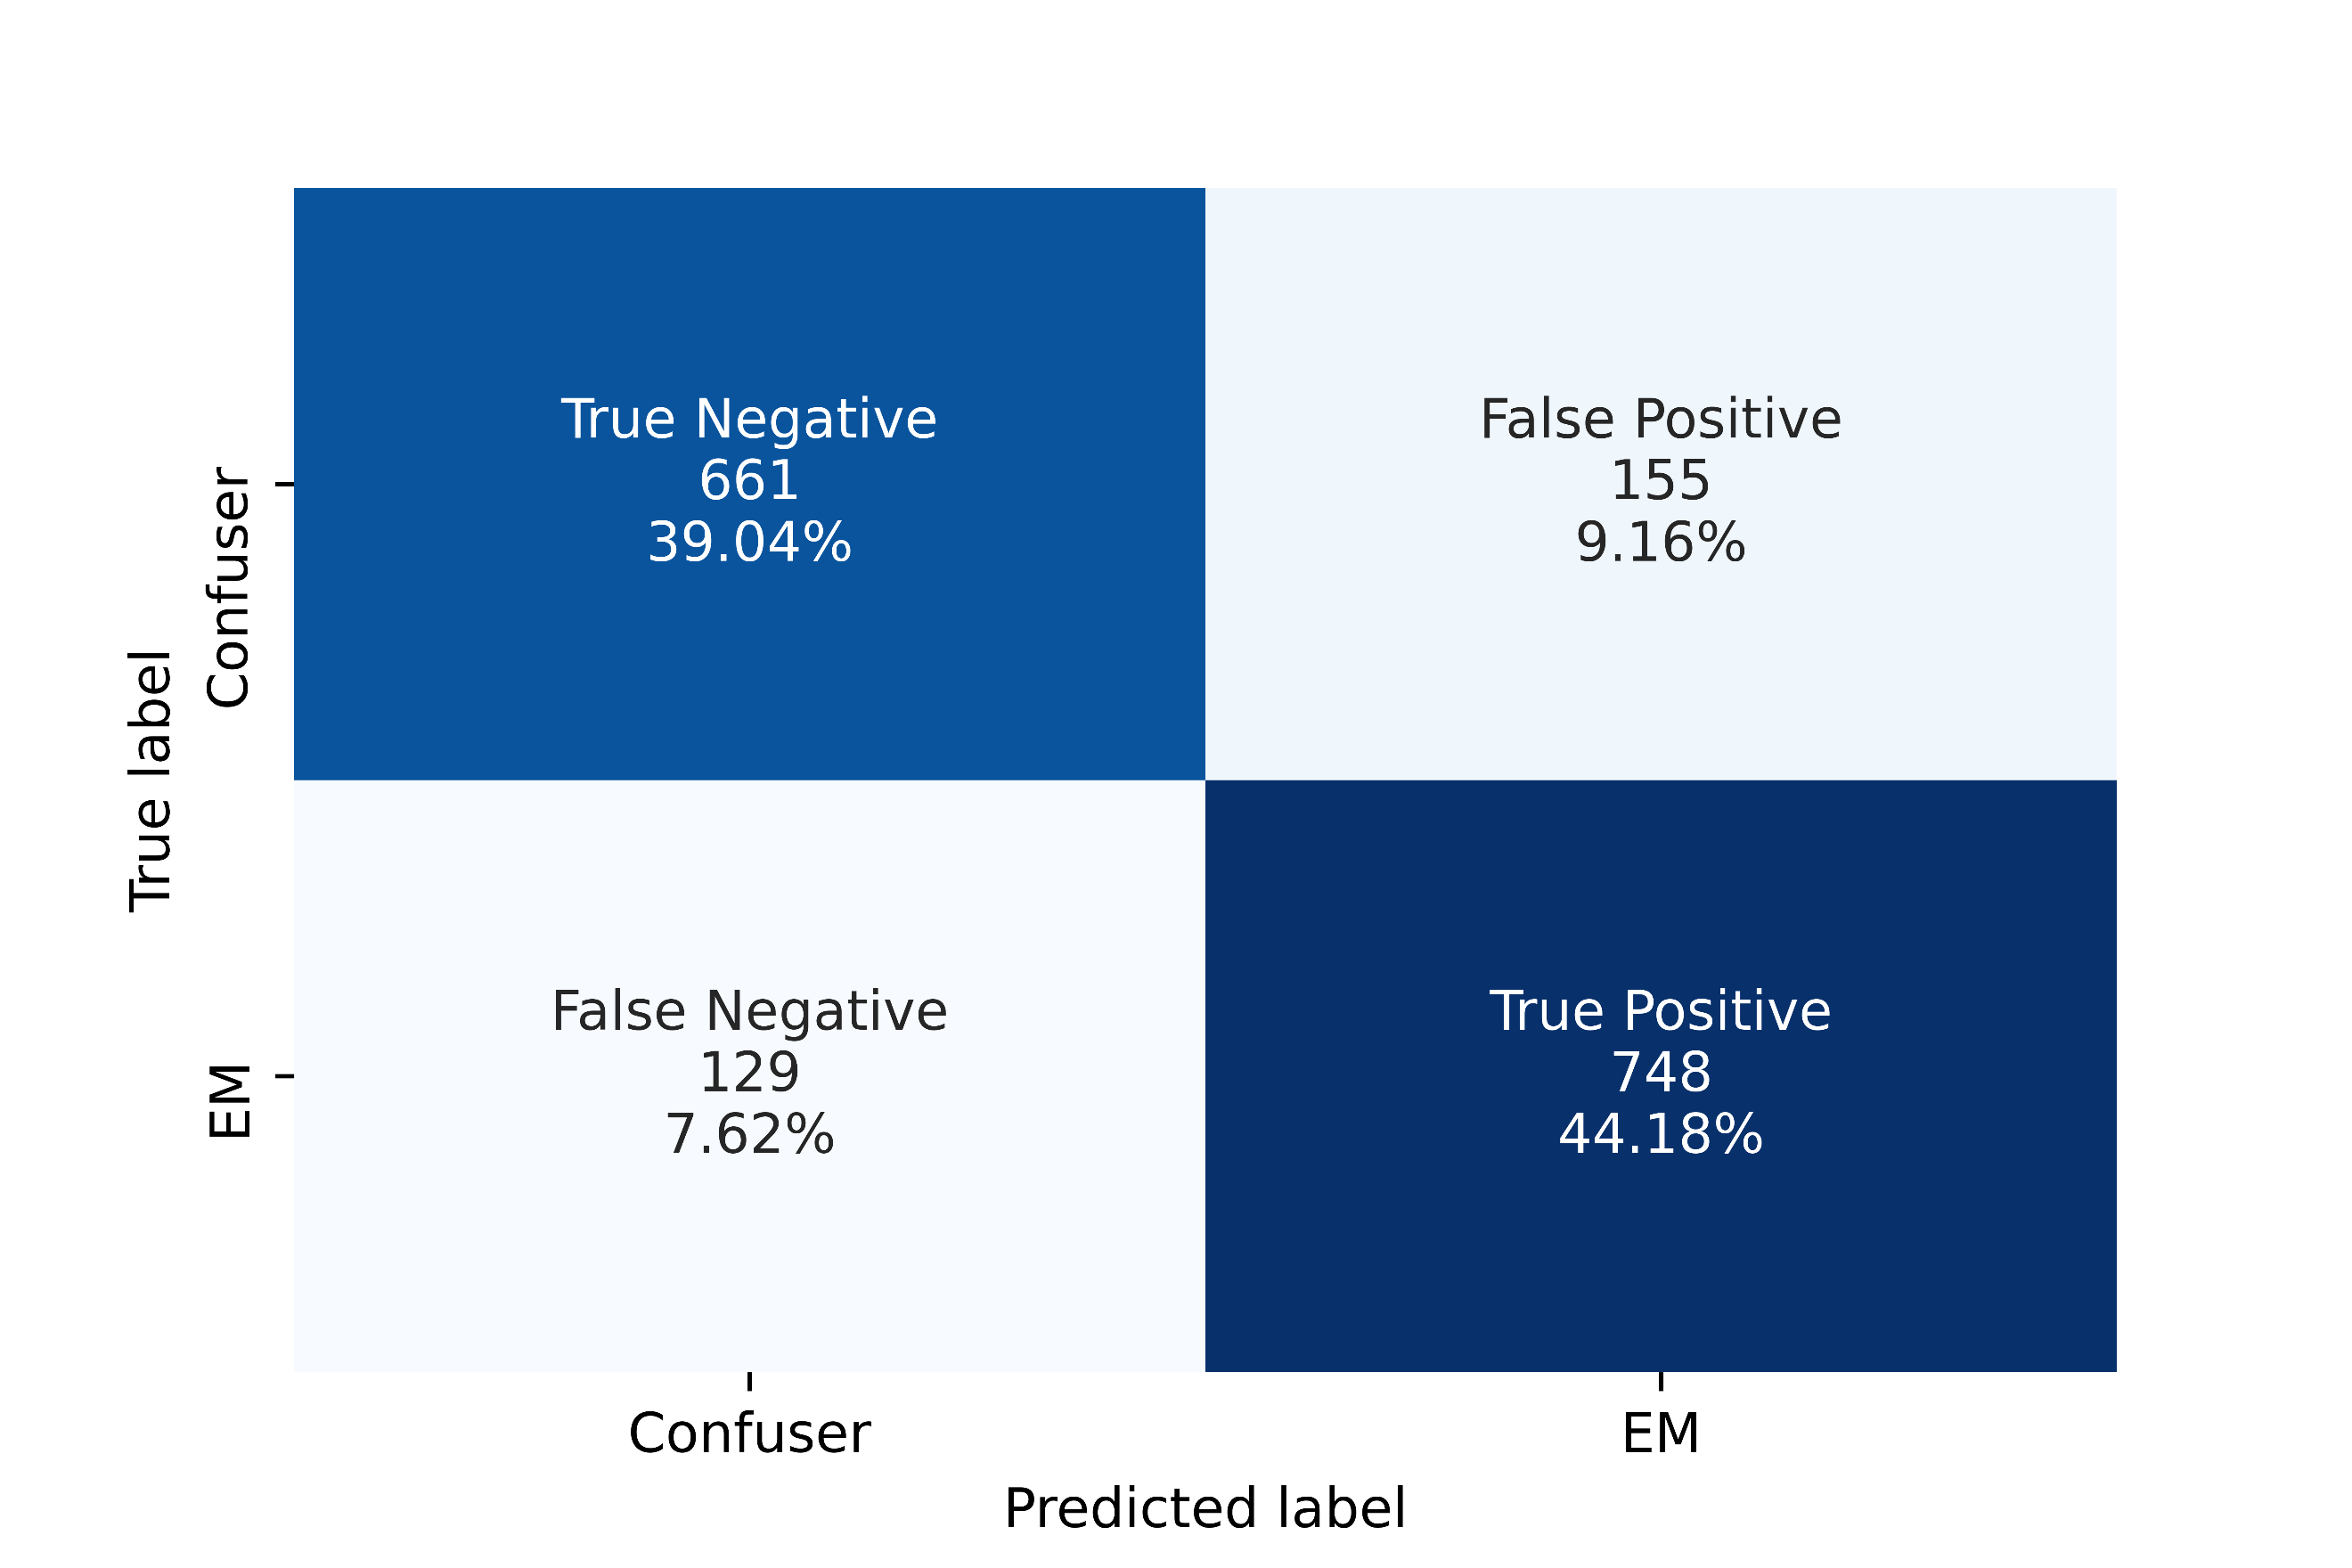
\includegraphics[width=\textwidth,keepaspectratio]{images/Supplement4/image61.png}
		\caption{Confusion matrix.}
	\end{subfigure}
	\caption{Five-fold cross-validation ROC curve and confusion matrix of ResNet50-IMG-FT141 model.}
\end{figure}

%%%%%%%%%%%%%%Break%%%%%%%%%%%%%%%%%%%%%%
\vfill\clearpage
\subsection{ResNet50-IMG-HAMFP-FT141}

\begin{table}[h!]
	\centering
	\caption{Five-fold cross-validation performance metrics of ResNet50-IMG-HAMFP-FT141 model.}
	\resizebox{\textwidth}{!}{%
		\begin{tabular}{llllllllllll}
			\toprule
			& \multicolumn{11}{c}{\textbf{Metric}}    \\ \cmidrule(lr){2-12} 
			\multicolumn{1}{l}{\textbf{Fold}} & \rotatebox{45}{Accuracy} 
			& \rotatebox{45}{Sensitivity} & \rotatebox{45}{Specificity} 
			& \rotatebox{45}{Precision} & \rotatebox{45}{NPV} & \rotatebox{45}{MCC} 
			& \rotatebox{45}{Kappa} 
			& \rotatebox{45}{LR$+$} & \rotatebox{45}{LR$-$} & \rotatebox{45}{F1-Score} 
			& \rotatebox{45}{AUC}  \\ \midrule
			fold1          & 81.18 & 89.73 & 71.93 & 77.57 & 86.62 & 0.6291 & 0.6206 & 3.1966 & 0.1428 & 0.8321 & 0.9061 \\
			fold2          & 83.58 & 85.55 & 81.48 & 83.15 & 84.08 & 0.6713 & 0.671  & 4.6197 & 0.1774 & 0.8433 & 0.9189 \\
			fold3          & 80.24 & 89.6  & 70.19 & 76.35 & 86.26 & 0.6118 & 0.6017 & 3.0052 & 0.1482 & 0.8245 & 0.8982 \\
			fold4          & 82.04 & 93.06 & 70.19 & 77.03 & 90.4  & 0.6531 & 0.6374 & 3.1215 & 0.0988 & 0.8429 & 0.9096 \\
			fold5          & 84.73 & 88.44 & 80.75 & 83.15 & 86.67 & 0.695  & 0.6935 & 4.5931 & 0.1432 & 0.8571 & 0.9236 \\\cmidrule(lr){1-12}
			average        & 82.35 & 89.28 & 74.91 & 79.45 & 86.81 & 0.6521 & 0.6448 & 3.7072 & 0.1421 & 0.84   & 0.9113 \\
			std. deviation & 1.62  & 2.42  & 5.11  & 3.05  & 2.03  & 0.0295 & 0.0333 & 0.7368 & 0.0251 & 0.0111 & 0.0091\\
			\bottomrule
		\end{tabular}%
	}
\end{table}


\begin{figure}[h!]
	\centering
	\begin{subfigure}[b]{0.49\textwidth}
		\centering
		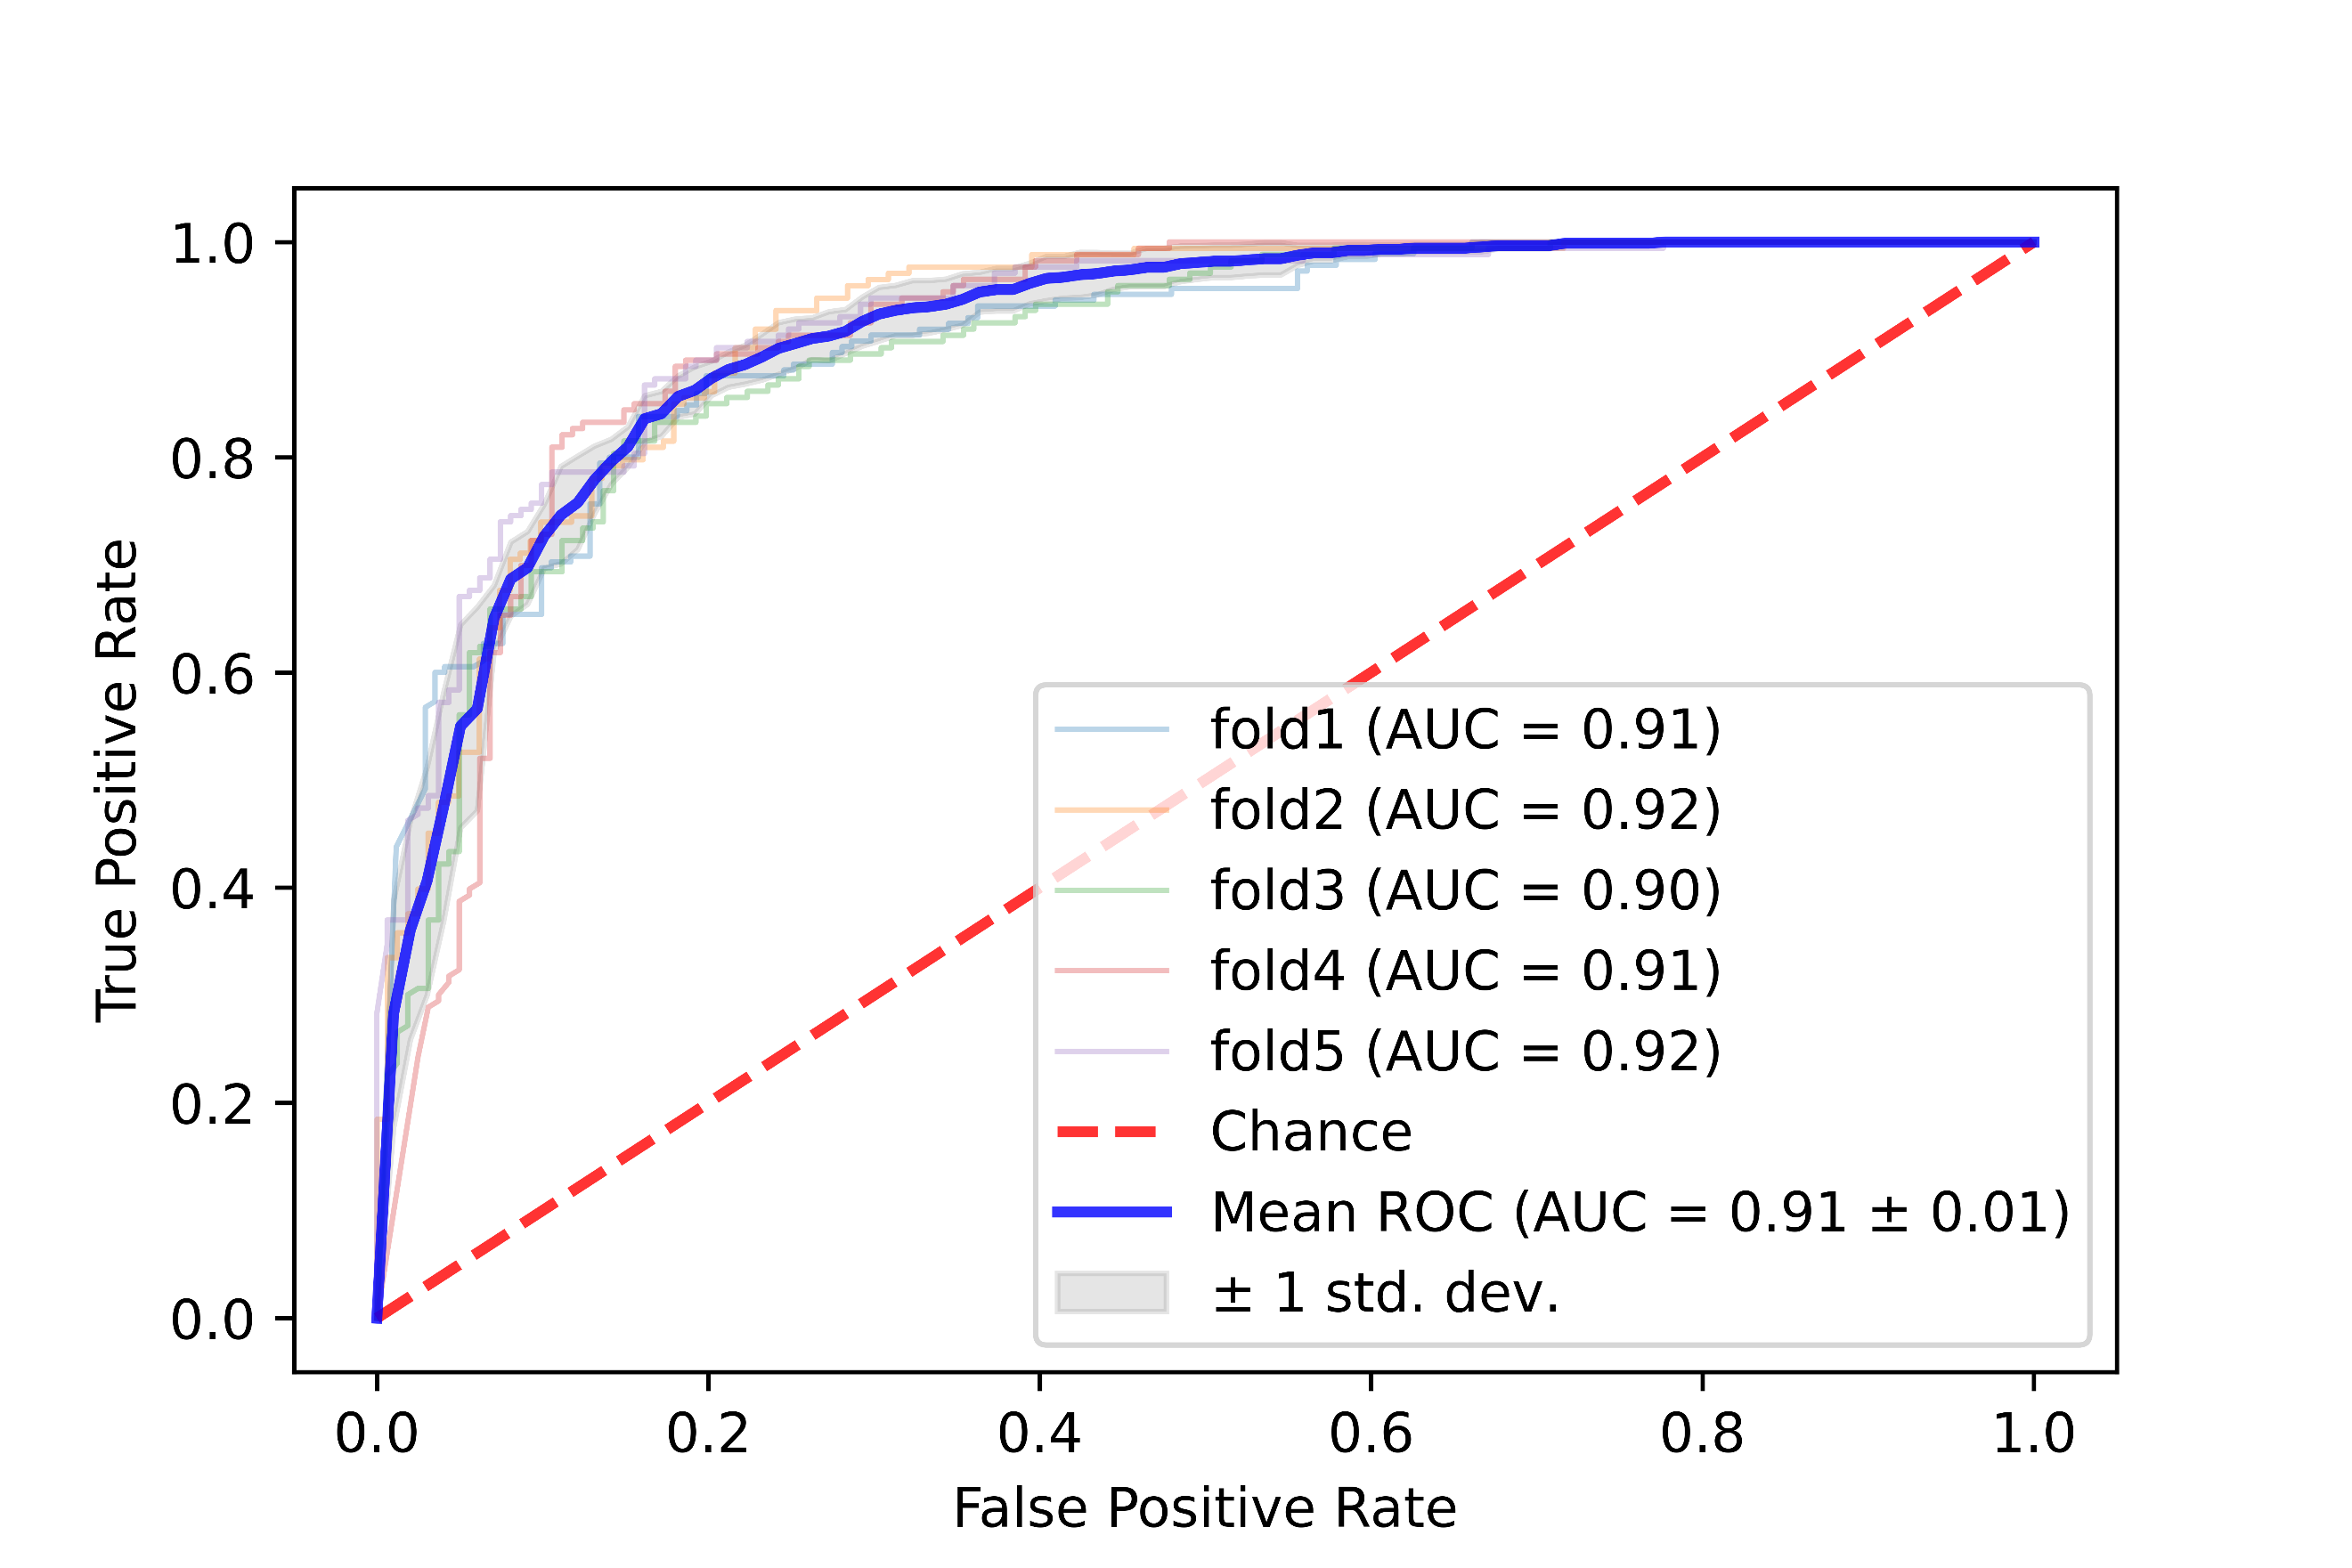
\includegraphics[width=\textwidth,keepaspectratio]{images/Supplement4/image62.png}
		\caption{ROC curve.}
	\end{subfigure}
	\hfill
	\begin{subfigure}[b]{0.49\textwidth}
		\centering
		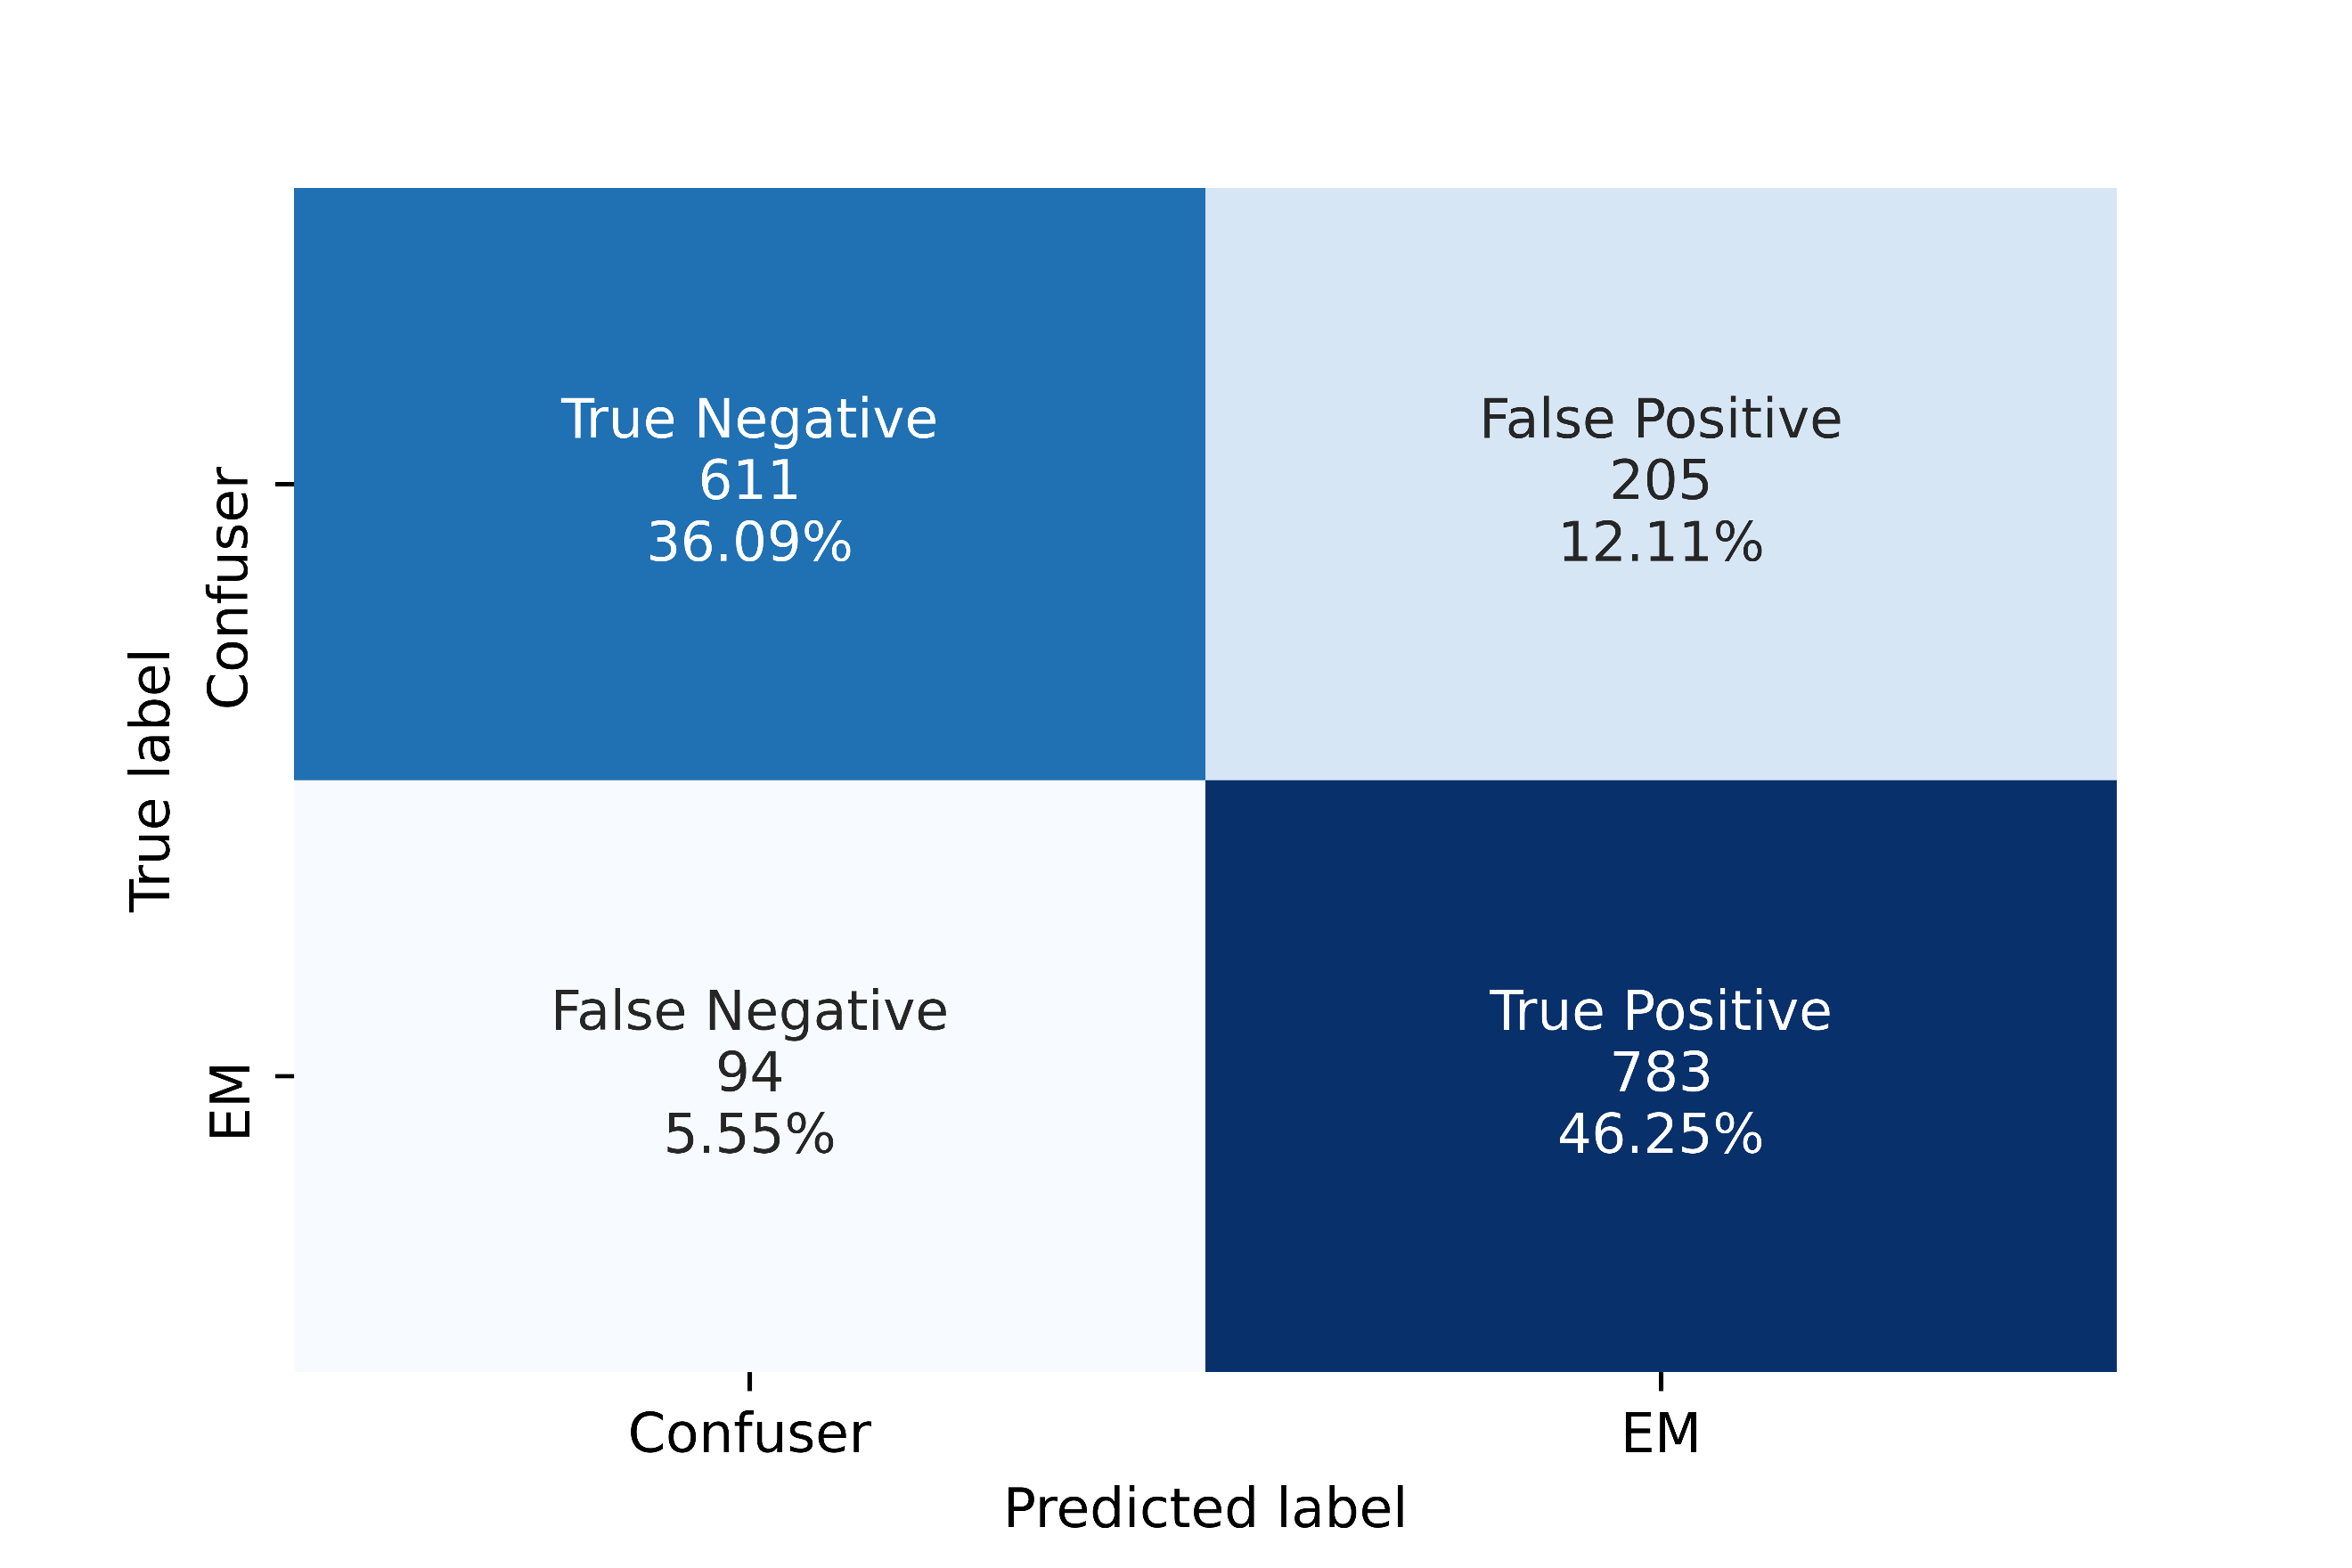
\includegraphics[width=\textwidth,keepaspectratio]{images/Supplement4/image68.png}
		\caption{Confusion matrix.}
	\end{subfigure}
	\caption{Five-fold cross-validation ROC curve and confusion matrix of ResNet50-IMG-HAMFP-FT141 model.}
\end{figure}

%%%%%%%%%%%%%%Break%%%%%%%%%%%%%%%%%%%%%%
\vfill\clearpage
\subsection{ResNet50-IMG-HAMPP-FT141/ ResNet50-141}

\begin{table}[h!]
	\centering
	\caption{Five-fold cross-validation performance metrics of ResNet50-IMG-HAMPP-FT141/ ResNet50-141 model.}
	\resizebox{\textwidth}{!}{%
		\begin{tabular}{llllllllllll}
			\toprule
			& \multicolumn{11}{c}{\textbf{Metric}}    \\ \cmidrule(lr){2-12} 
			\multicolumn{1}{l}{\textbf{Fold}} & \rotatebox{45}{Accuracy} 
			& \rotatebox{45}{Sensitivity} & \rotatebox{45}{Specificity} 
			& \rotatebox{45}{Precision} & \rotatebox{45}{NPV} & \rotatebox{45}{MCC} 
			& \rotatebox{45}{Kappa} 
			& \rotatebox{45}{LR$+$} & \rotatebox{45}{LR$-$} & \rotatebox{45}{F1-Score} 
			& \rotatebox{45}{AUC}  \\ \midrule
			fold1          & 83.15 & 86.49 & 79.53 & 82.05 & 84.47 & 0.6627 & 0.6617 & 4.2255 & 0.1699 & 0.8421 & 0.9072 \\
			fold2          & 83.28 & 87.86 & 78.4  & 81.28 & 85.81 & 0.6667 & 0.6644 & 4.0667 & 0.1548 & 0.8444 & 0.9109 \\
			fold3          & 83.53 & 90.75 & 75.78 & 80.1  & 88.41 & 0.6751 & 0.6686 & 3.7464 & 0.1221 & 0.8509 & 0.9107 \\
			fold4          & 85.93 & 87.28 & 84.47 & 85.8  & 86.08 & 0.7181 & 0.718  & 5.621  & 0.1505 & 0.8653 & 0.9323 \\
			fold5          & 86.23 & 87.28 & 85.09 & 86.29 & 86.16 & 0.7241 & 0.7241 & 5.8553 & 0.1494 & 0.8678 & 0.9335 \\\cmidrule(lr){1-12}
			average        & 84.42 & 87.93 & 80.65 & 83.1  & 86.19 & 0.6893 & 0.6874 & 4.703  & 0.1493 & 0.8541 & 0.9189 \\
			std. deviation & 1.36  & 1.47  & 3.59  & 2.49  & 1.27  & 0.0263 & 0.0277 & 0.8624 & 0.0155 & 0.0106 & 0.0115\\
			\bottomrule
		\end{tabular}%
	}
\end{table}


\begin{figure}[h!]
	\centering
	\begin{subfigure}[b]{0.49\textwidth}
		\centering
		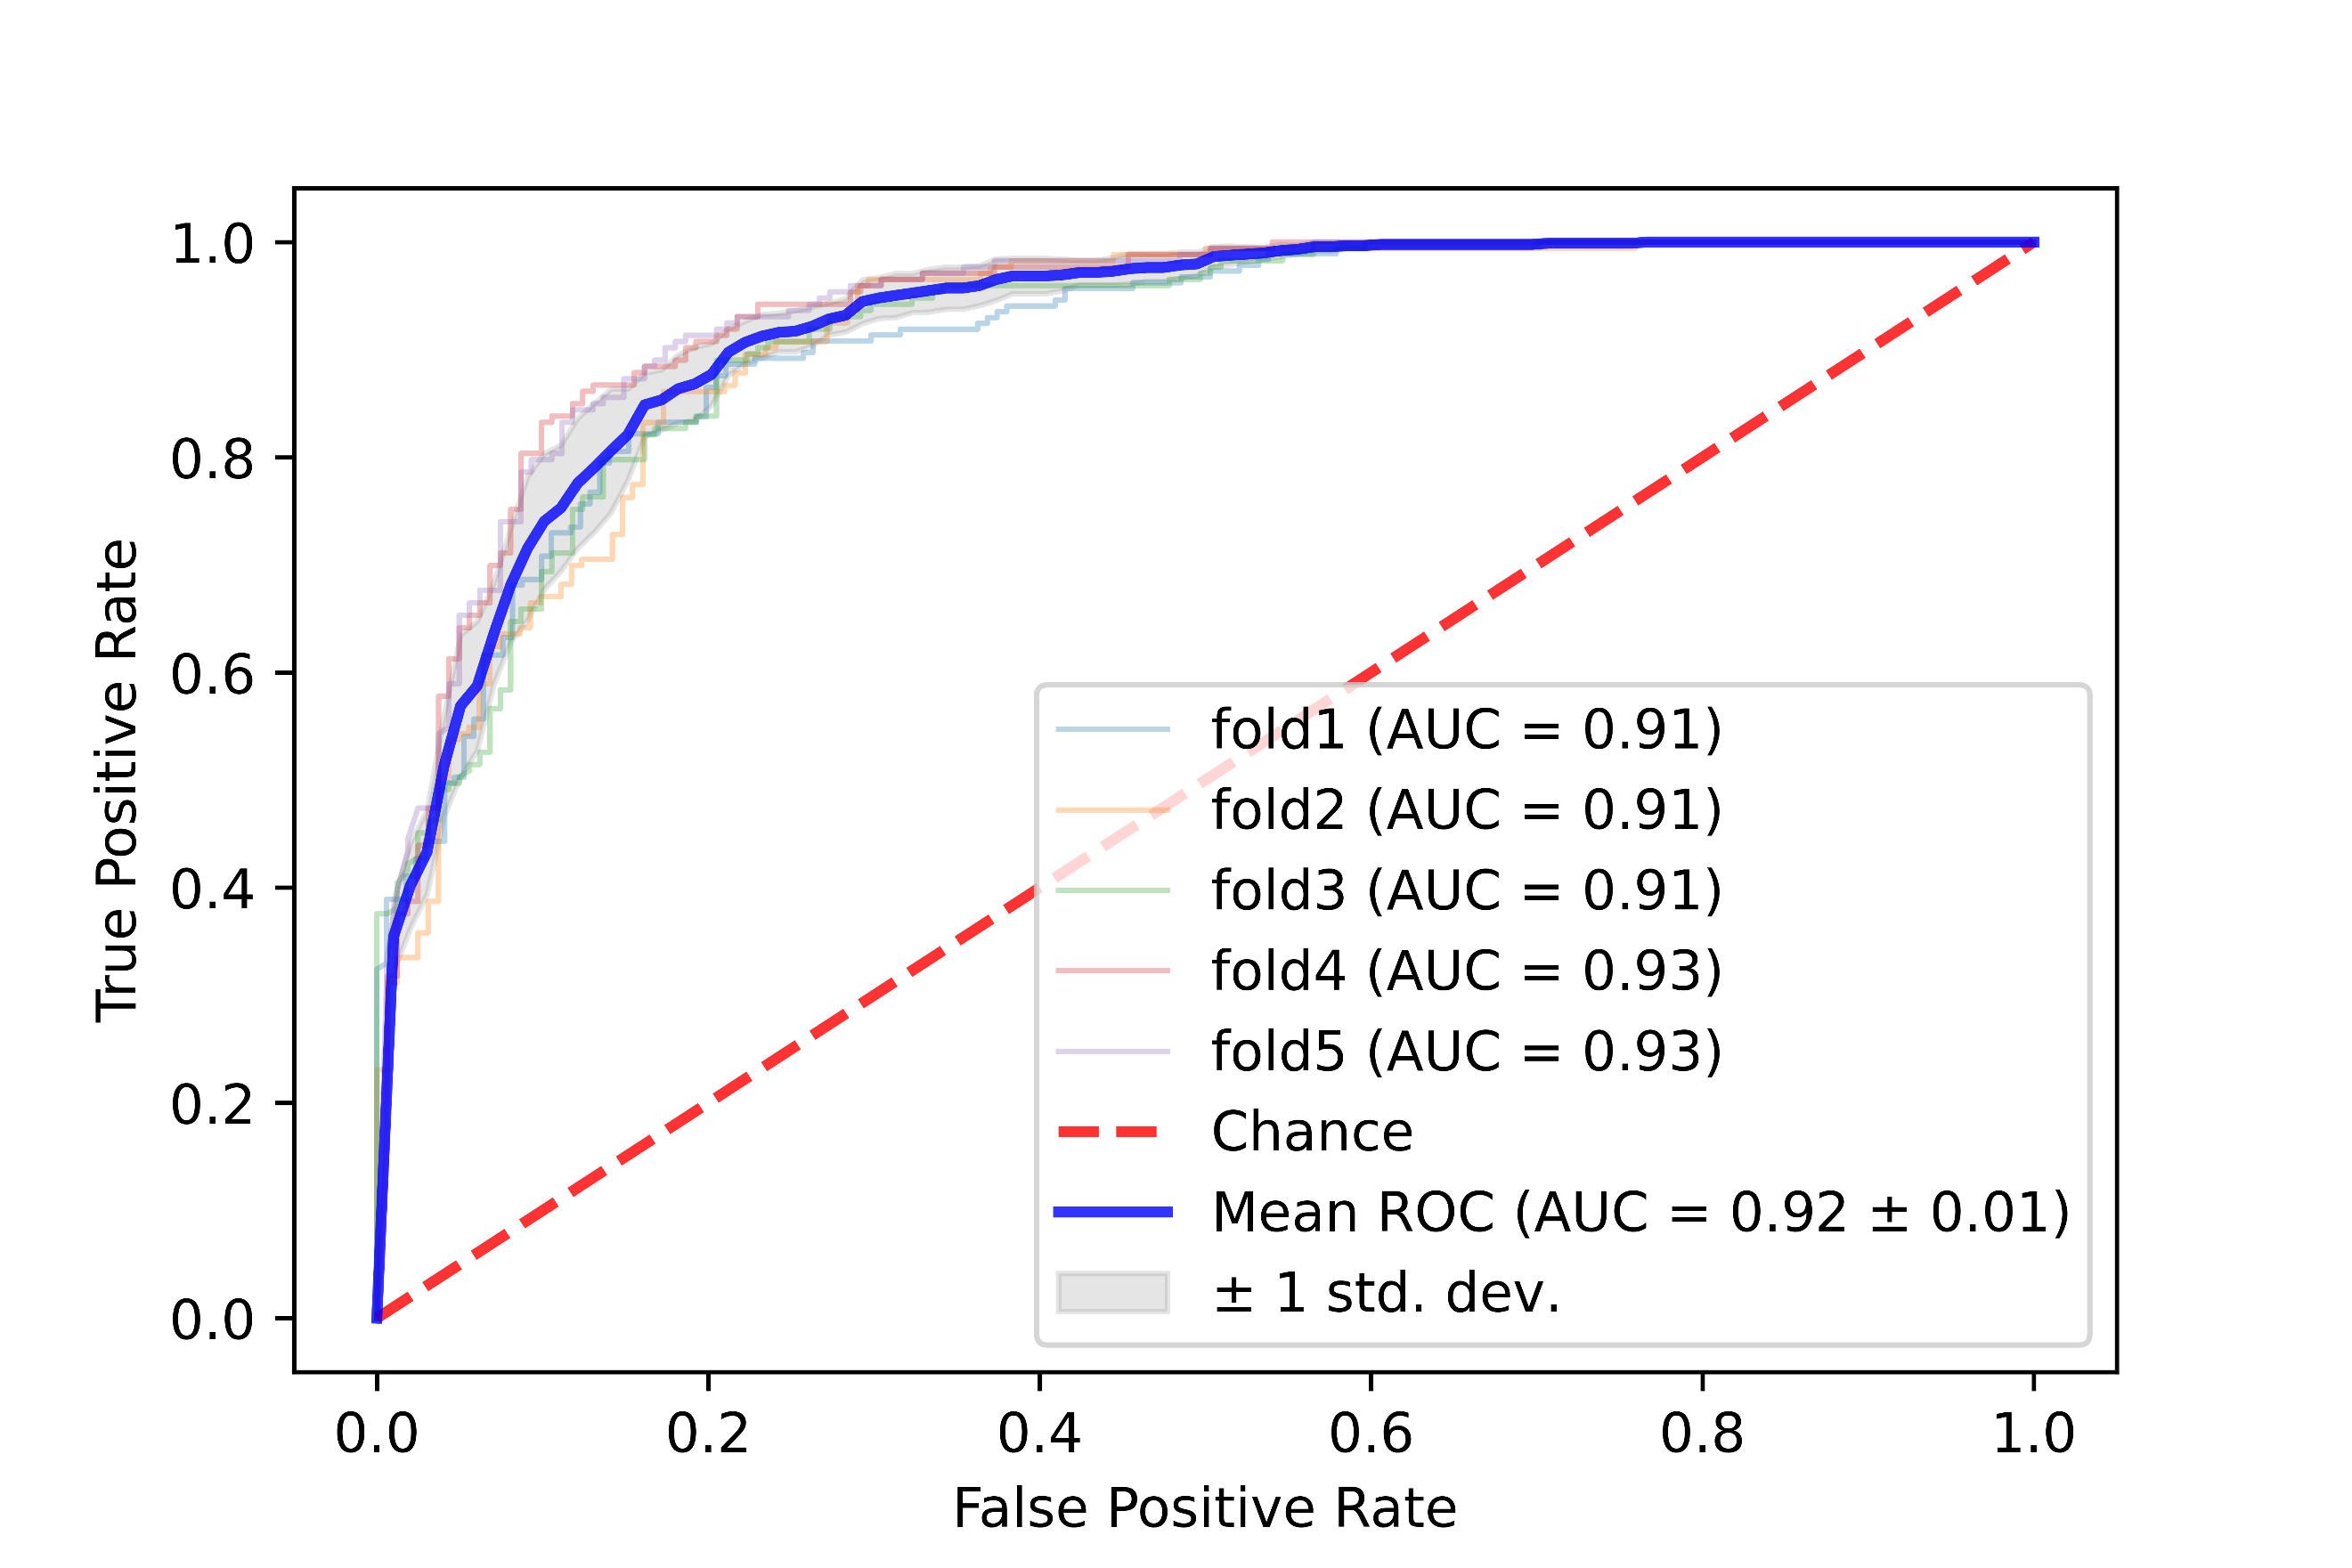
\includegraphics[width=\textwidth,keepaspectratio]{images/Supplement4/image69.png}
		\caption{ROC curve.}
	\end{subfigure}
	\hfill
	\begin{subfigure}[b]{0.49\textwidth}
		\centering
		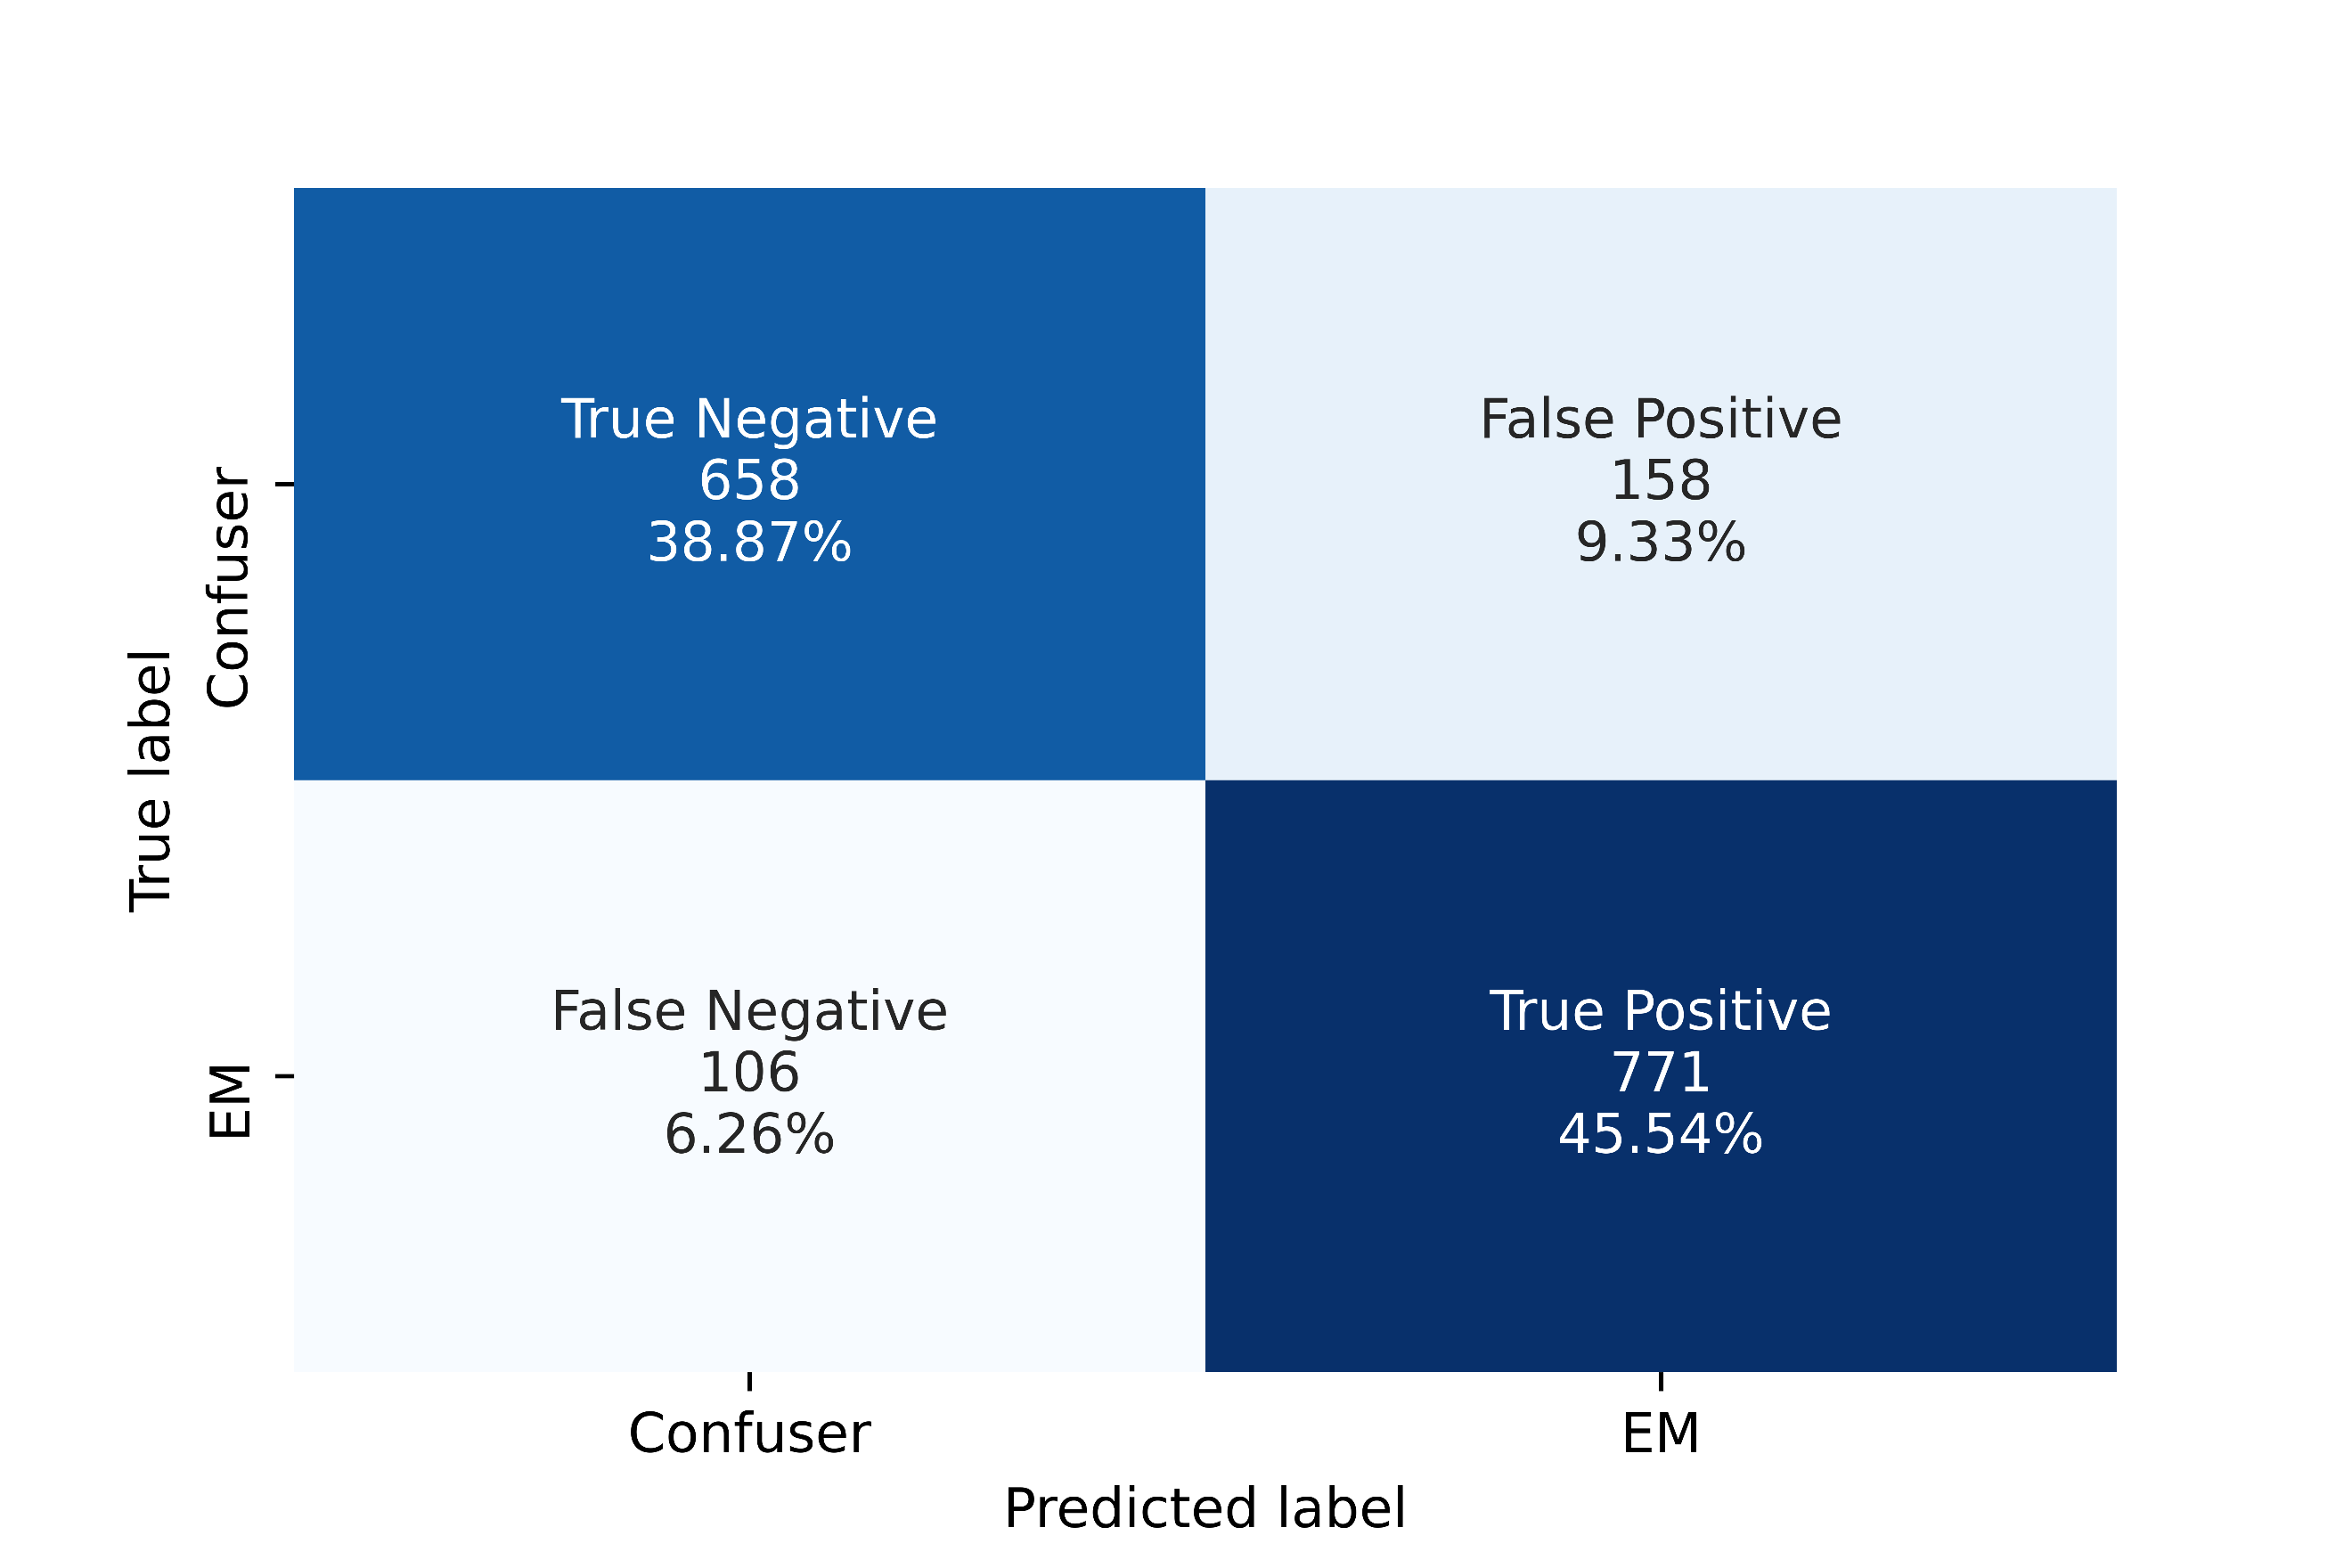
\includegraphics[width=\textwidth,keepaspectratio]{images/Supplement4/image75.png}
		\caption{Confusion matrix.}
	\end{subfigure}
	\caption{Five-fold cross-validation ROC curve and confusion matrix of ResNet50-IMG-HAMPP-FT141/ ResNet50-141 model.}
\end{figure}

%%%%%%%%%%%%%%Break%%%%%%%%%%%%%%%%%%%%%%
\vfill\clearpage
\subsection{ResNet101-150}

\begin{table}[h!]
	\centering
	\caption{Five-fold cross-validation performance metrics of ResNet101-150 model.}
	\resizebox{\textwidth}{!}{%
		\begin{tabular}{llllllllllll}
			\toprule
			& \multicolumn{11}{c}{\textbf{Metric}}    \\ \cmidrule(lr){2-12} 
			\multicolumn{1}{l}{\textbf{Fold}} & \rotatebox{45}{Accuracy} & 
			\rotatebox{45}{Sensitivity} & \rotatebox{45}{Specificity} & 
			\rotatebox{45}{Precision} & \rotatebox{45}{NPV} & \rotatebox{45}{MCC} & 
			\rotatebox{45}{Kappa} & \rotatebox{45}{LR$+$} & \rotatebox{45}{LR$-$} & 
			\rotatebox{45}{F1-Score} & \rotatebox{45}{AUC}  \\ \midrule
			fold1          & 82.3  & 84.86 & 79.53 & 81.77 & 82.93 & 0.6455 & 0.645  & 4.1463 & 0.1903 & 0.8329 & 0.9076 \\
			fold2          & 82.69 & 80.92 & 84.57 & 84.85 & 80.59 & 0.6546 & 0.6539 & 5.2439 & 0.2256 & 0.8284 & 0.8982 \\
			fold3          & 82.34 & 85.55 & 78.88 & 81.32 & 83.55 & 0.6465 & 0.6456 & 4.051  & 0.1832 & 0.8338 & 0.8958 \\
			fold4          & 86.23 & 88.44 & 83.85 & 85.47 & 87.1  & 0.7243 & 0.7238 & 5.4764 & 0.1379 & 0.8693 & 0.9214 \\
			fold5          & 79.64 & 78.61 & 80.75 & 81.44 & 77.84 & 0.5932 & 0.5928 & 4.0828 & 0.2649 & 0.8    & 0.8992 \\\cmidrule(lr){1-12}
			average        & 82.64 & 83.68 & 81.52 & 82.97 & 82.4  & 0.6528 & 0.6522 & 4.6001 & 0.2004 & 0.8329 & 0.9044 \\
			std. deviation & 2.1   & 3.49  & 2.29  & 1.8   & 3.09  & 0.0419 & 0.0418 & 0.6257 & 0.0427 & 0.022  & 0.0094\\
			\bottomrule
		\end{tabular}%
	}
\end{table}


\begin{figure}[h!]
	\centering
	\begin{subfigure}[b]{0.49\textwidth}
		\centering
		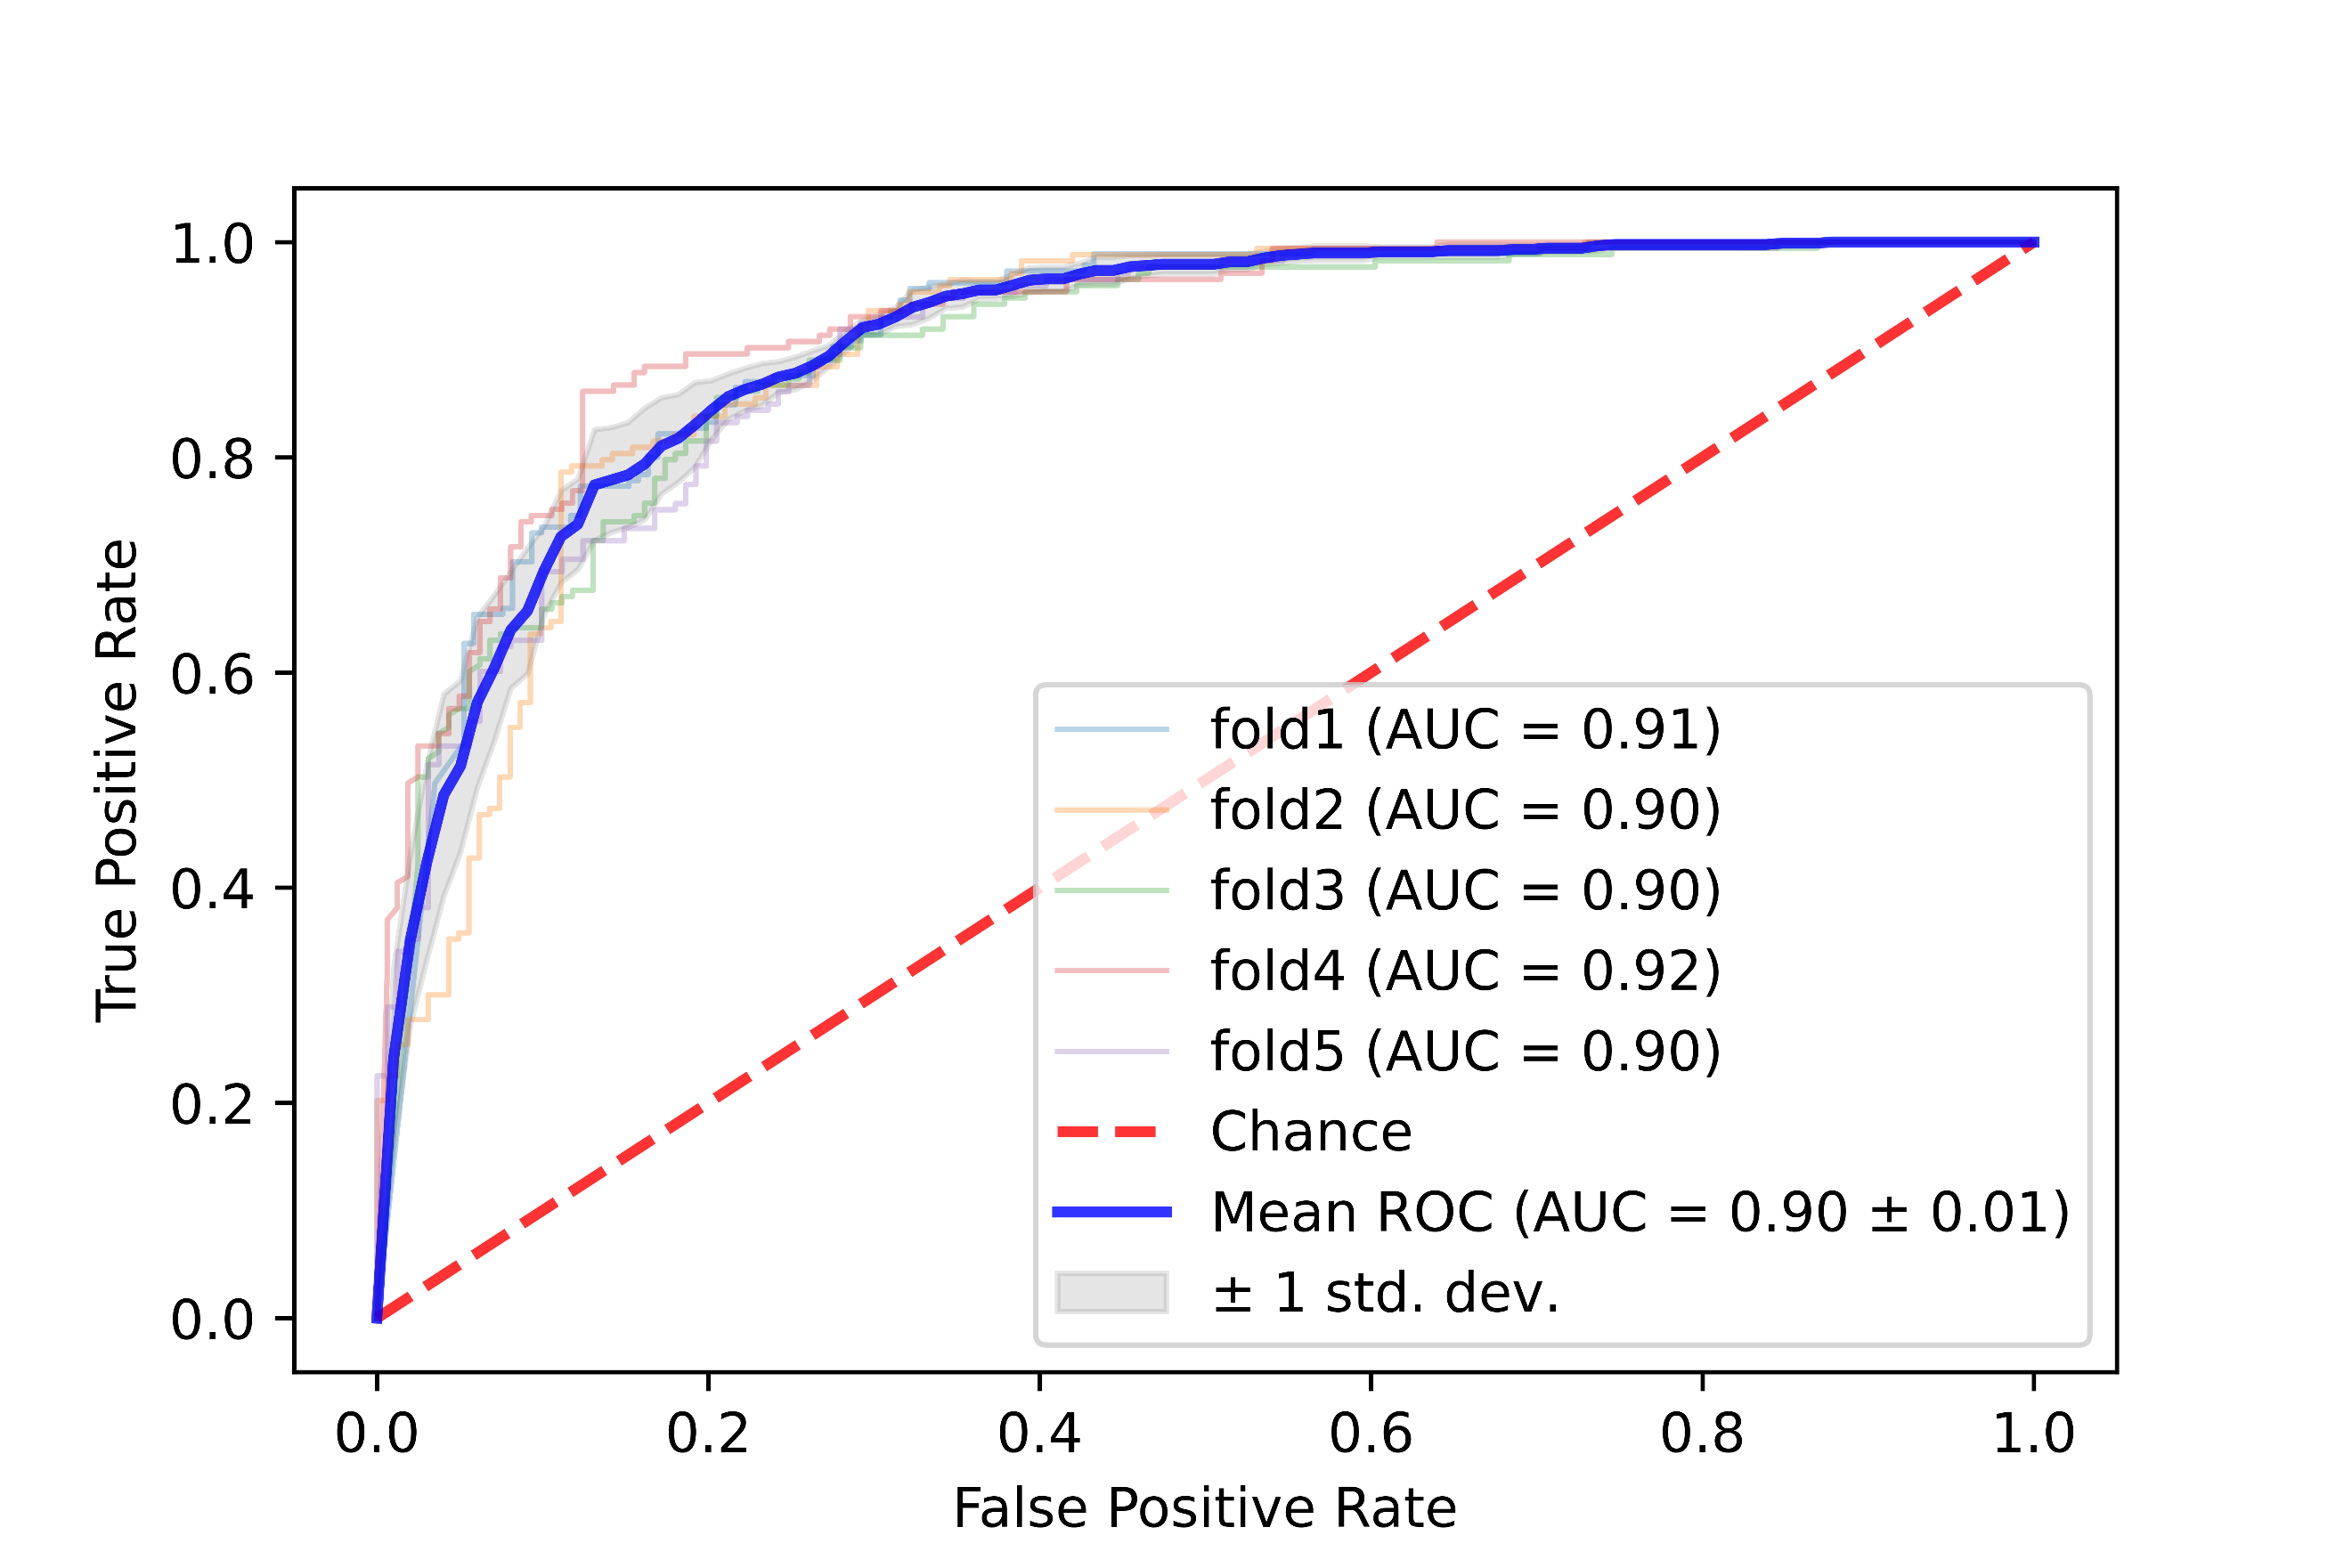
\includegraphics[width=\textwidth,keepaspectratio]{images/Supplement4/image76.png}
		\caption{ROC curve.}
	\end{subfigure}
	\hfill
	\begin{subfigure}[b]{0.49\textwidth}
		\centering
		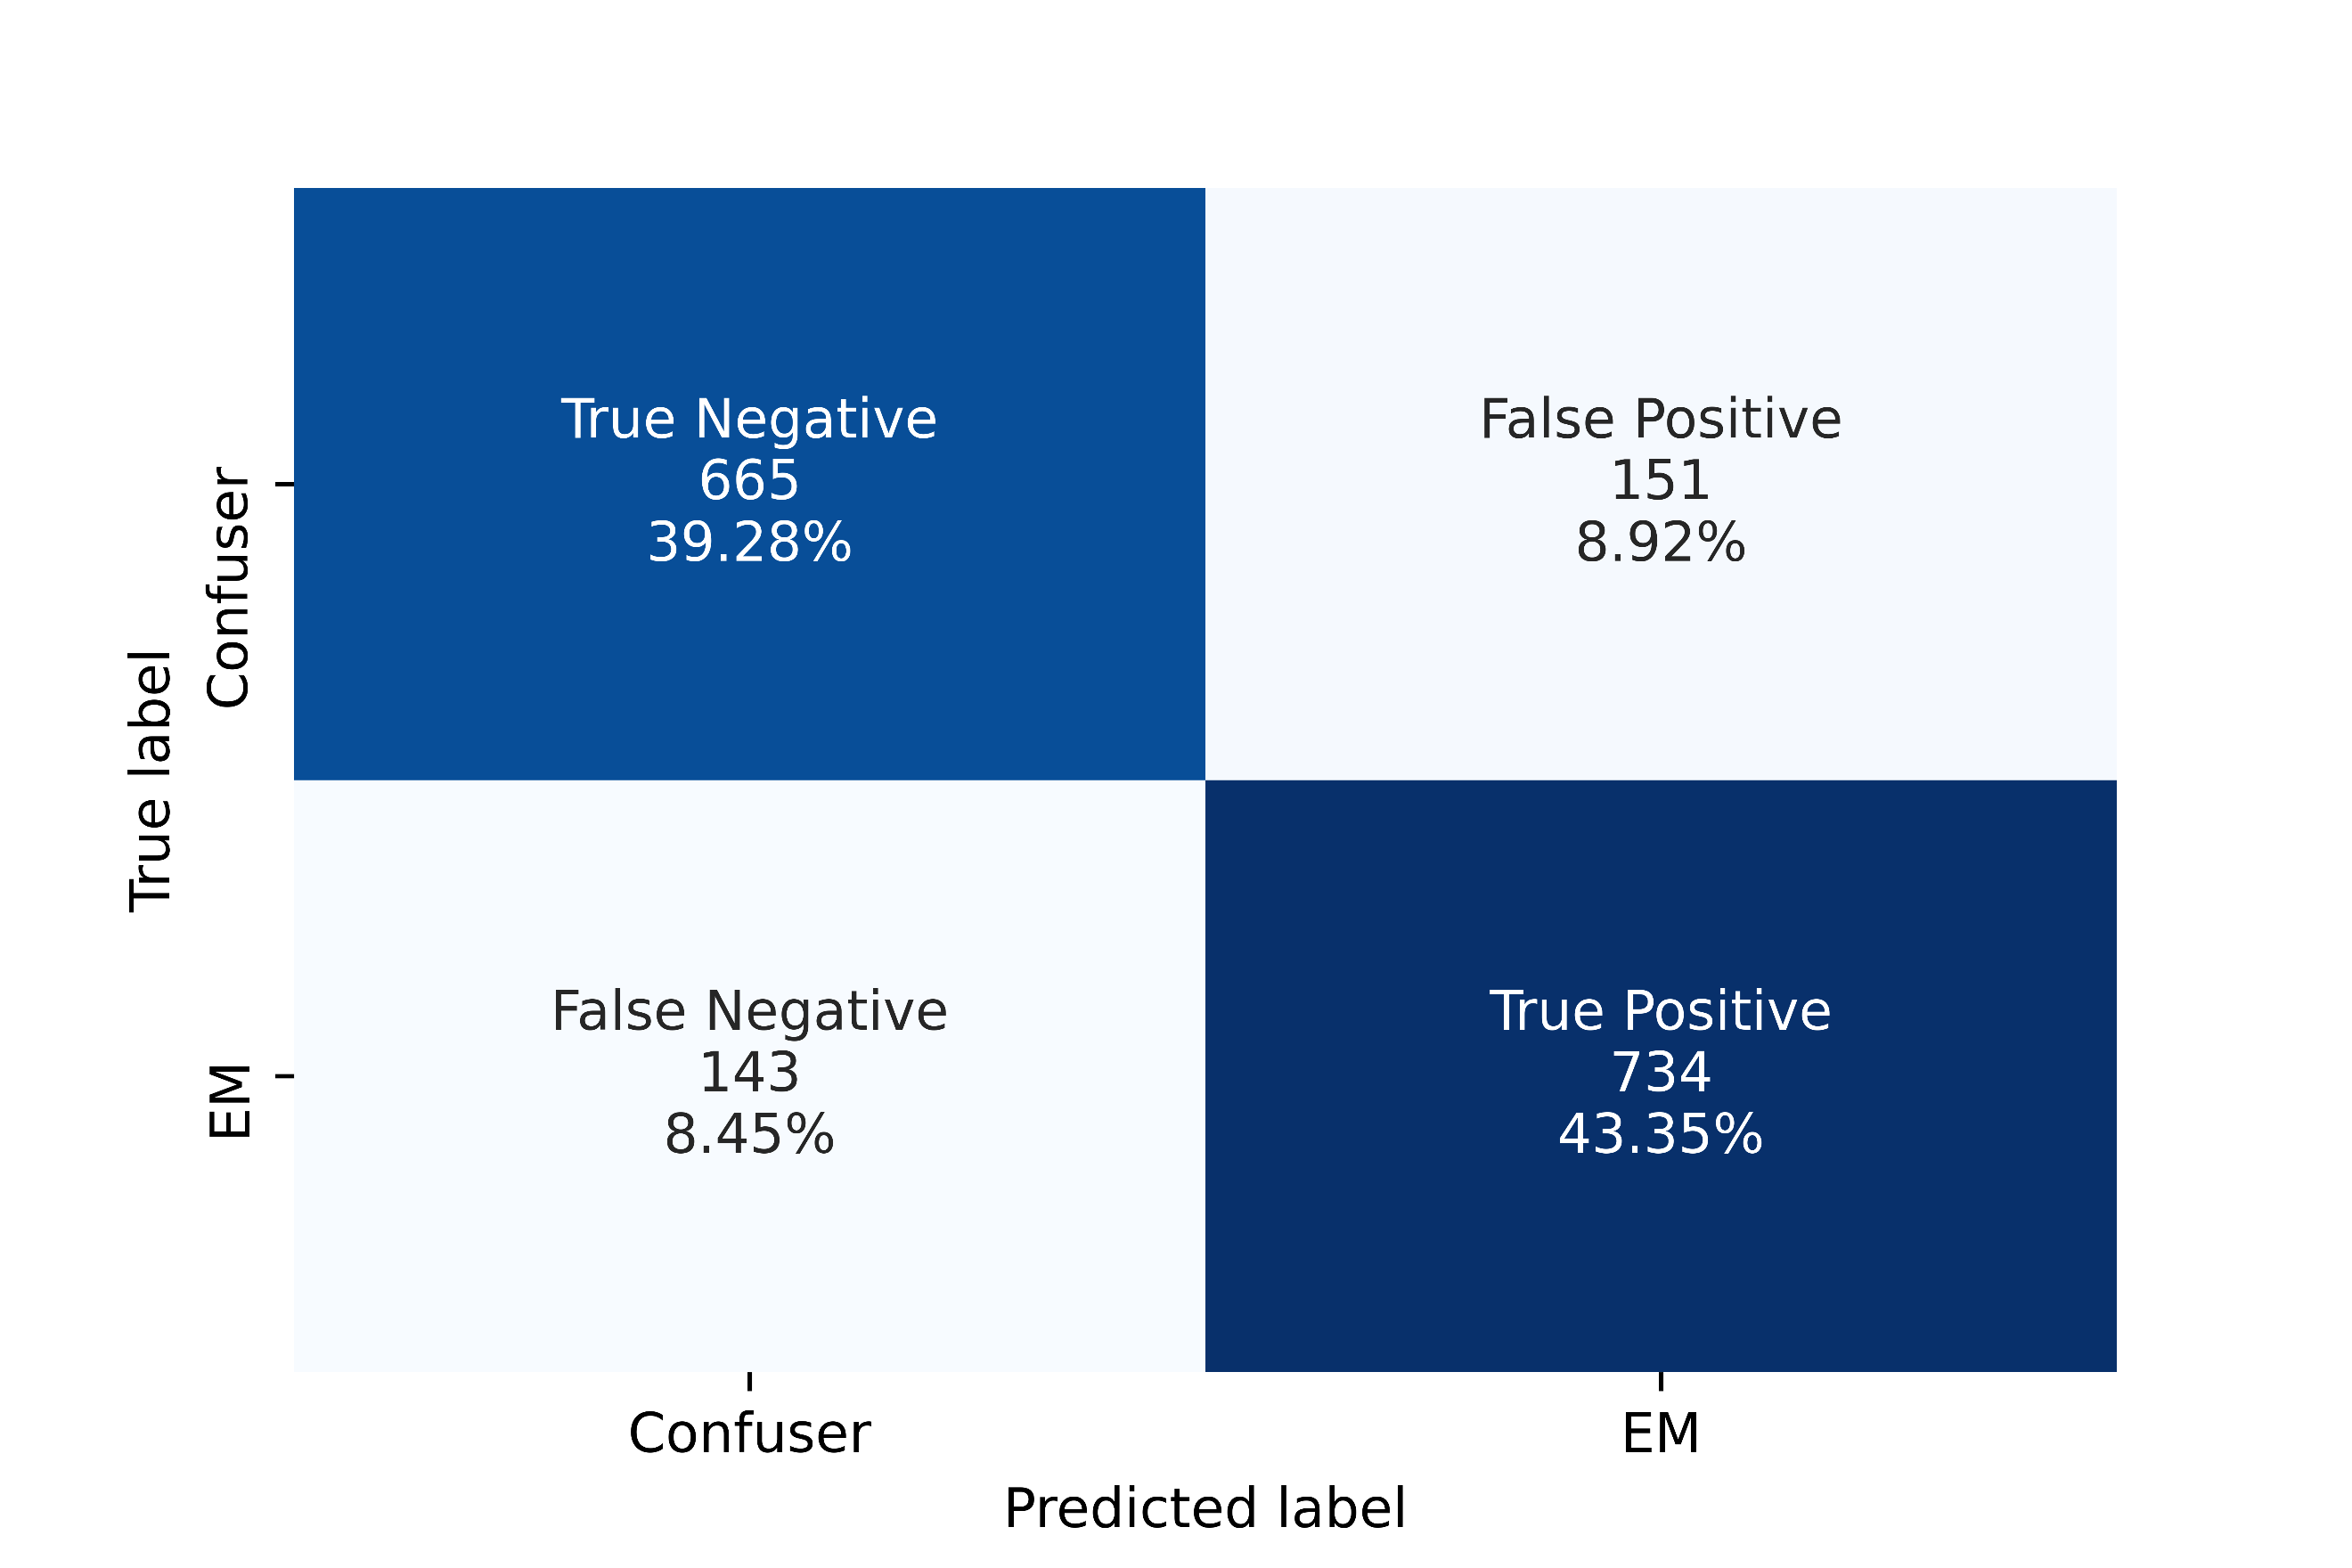
\includegraphics[width=\textwidth,keepaspectratio]{images/Supplement4/image82.png}
		\caption{Confusion matrix.}
	\end{subfigure}
	\caption{Five-fold cross-validation ROC curve and confusion matrix of ResNet101-150 model.}
\end{figure}

%%%%%%%%%%%%%%Break%%%%%%%%%%%%%%%%%%%%%%
\vfill\clearpage
\subsection{ResNet50V2-105}

\begin{table}[h!]
	\centering
	\caption{Five-fold cross-validation performance metrics of ResNet50V2-105 model.}
	\resizebox{\textwidth}{!}{%
		\begin{tabular}{llllllllllll}
			\toprule
			& \multicolumn{11}{c}{\textbf{Metric}}    \\ \cmidrule(lr){2-12} 
			\multicolumn{1}{l}{\textbf{Fold}} & \rotatebox{45}{Accuracy} & 
			\rotatebox{45}{Sensitivity} & \rotatebox{45}{Specificity} & 
			\rotatebox{45}{Precision} & \rotatebox{45}{NPV} & \rotatebox{45}{MCC} & 
			\rotatebox{45}{Kappa} & \rotatebox{45}{LR$+$} & \rotatebox{45}{LR$-$} & 
			\rotatebox{45}{F1-Score} & \rotatebox{45}{AUC}  \\ \midrule
			fold1          & 80.06 & 84.86 & 74.85 & 78.5  & 82.05 & 0.6013 & 0.5992 & 3.3749 & 0.2022 & 0.8156 & 0.8761 \\
			fold2          & 85.07 & 84.97 & 85.19 & 85.96 & 84.15 & 0.7013 & 0.7013 & 5.7355 & 0.1764 & 0.8547 & 0.9103 \\
			fold3          & 80.24 & 90.75 & 68.94 & 75.85 & 87.4  & 0.6145 & 0.6014 & 2.9222 & 0.1341 & 0.8263 & 0.8999 \\
			fold4          & 81.74 & 80.35 & 83.23 & 83.73 & 79.76 & 0.6354 & 0.6348 & 4.7911 & 0.2361 & 0.8201 & 0.9128 \\
			fold5          & 84.73 & 86.71 & 82.61 & 84.27 & 85.26 & 0.6942 & 0.6939 & 4.9855 & 0.1609 & 0.8547 & 0.9076 \\\cmidrule(lr){1-12}
			average        & 82.37 & 85.53 & 78.96 & 81.66 & 83.72 & 0.6493 & 0.6461 & 4.3618 & 0.1819 & 0.8343 & 0.9013 \\
			std. deviation & 2.15  & 3.35  & 6.13  & 3.83  & 2.63  & 0.0411 & 0.0439 & 1.0495 & 0.0349 & 0.017  & 0.0133\\
			\bottomrule
		\end{tabular}%
	}
\end{table}


\begin{figure}[h!]
	\centering
	\begin{subfigure}[b]{0.49\textwidth}
		\centering
		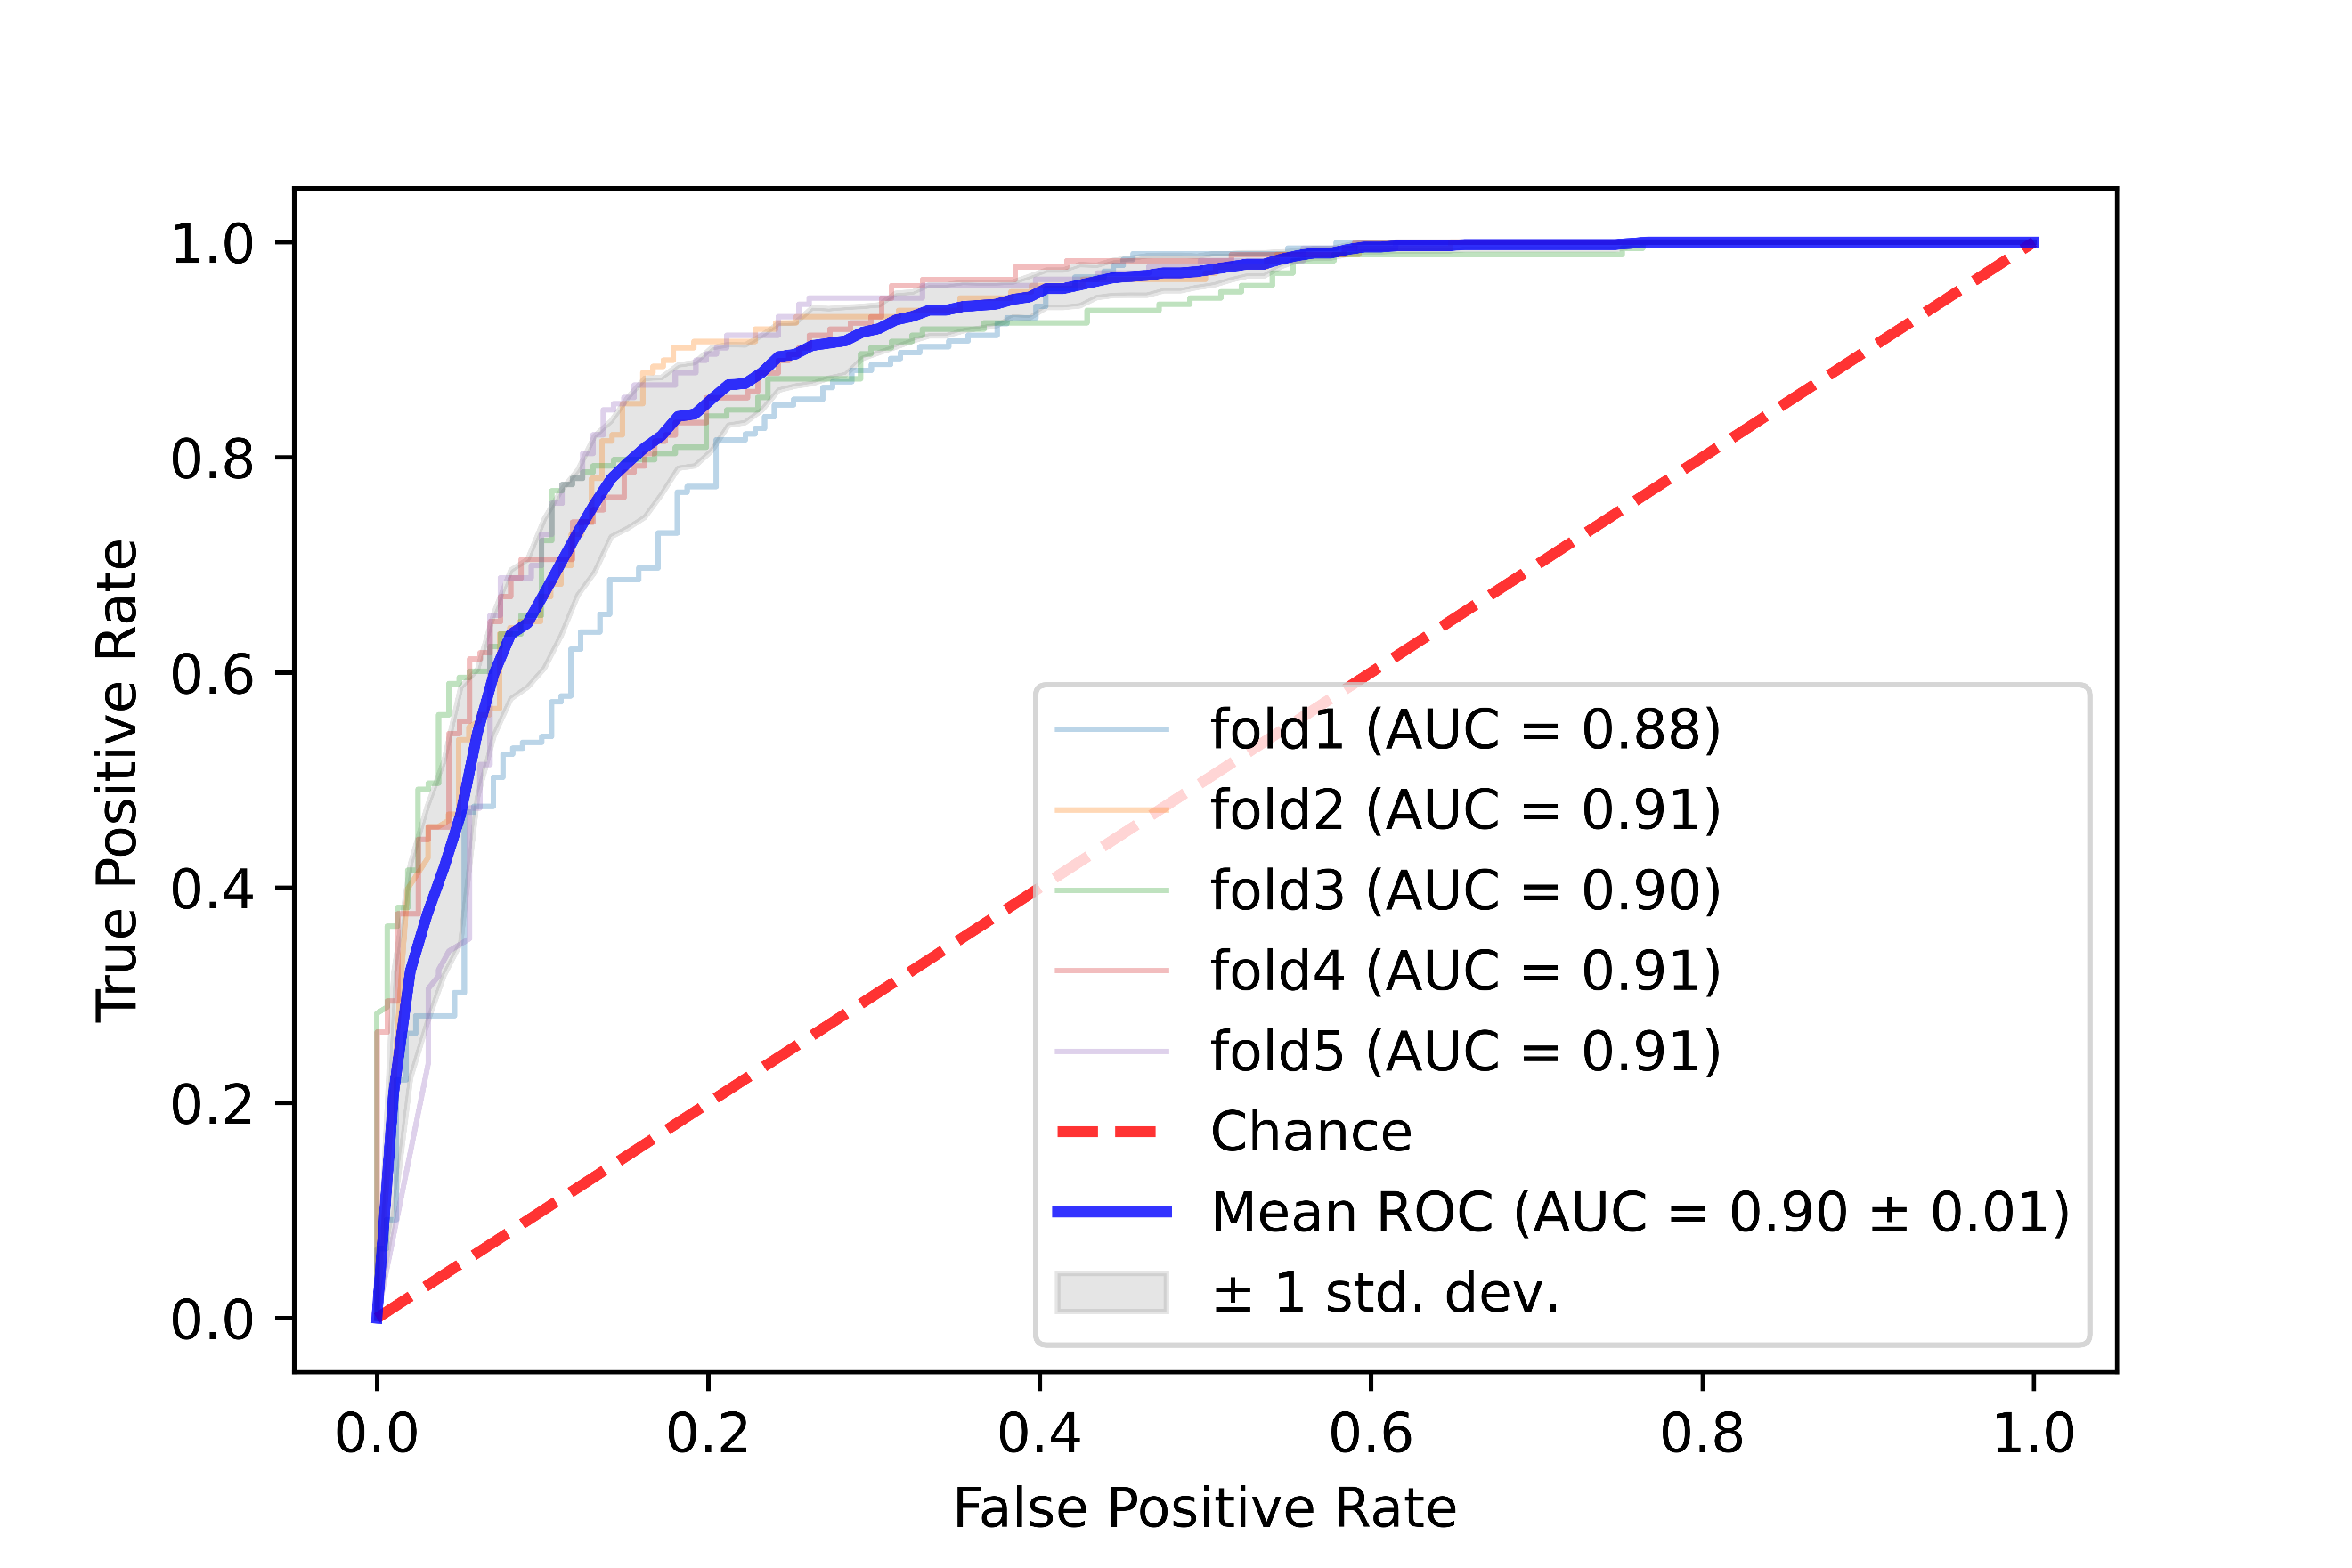
\includegraphics[width=\textwidth,keepaspectratio]{images/Supplement4/image83.png}
		\caption{ROC curve.}
	\end{subfigure}
	\hfill
	\begin{subfigure}[b]{0.49\textwidth}
		\centering
		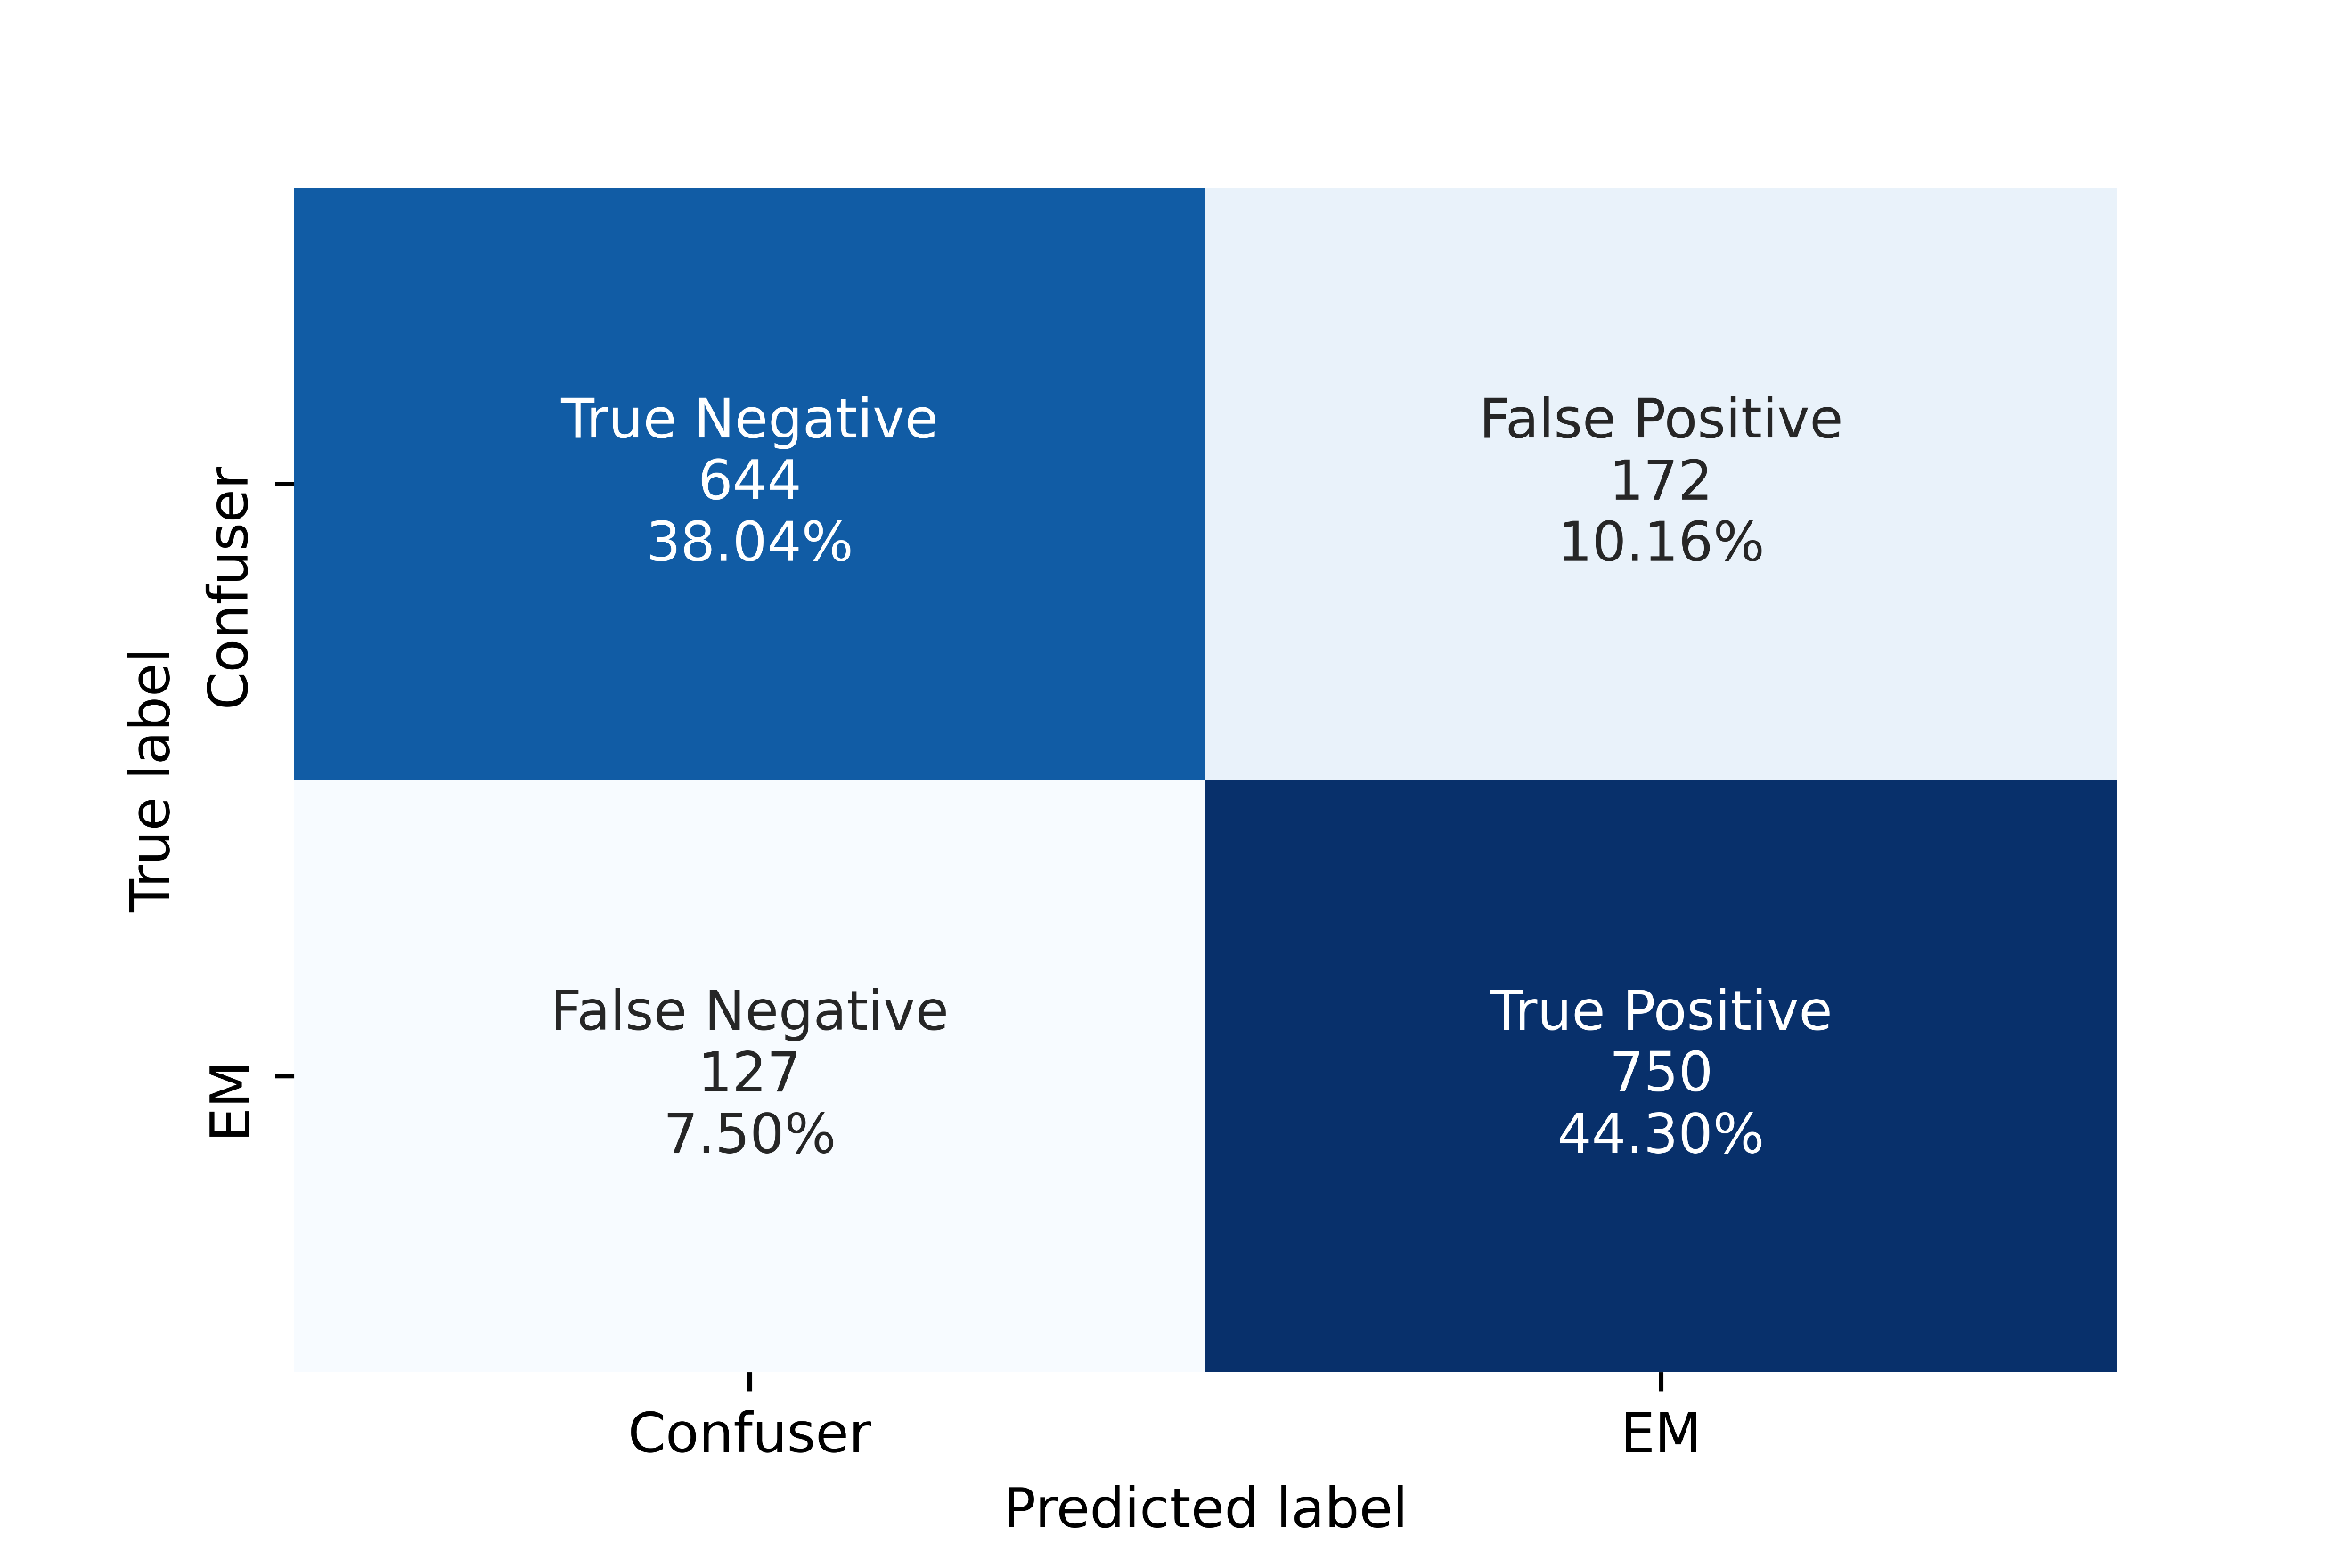
\includegraphics[width=\textwidth,keepaspectratio]{images/Supplement4/image89.png}
		\caption{Confusion matrix.}
	\end{subfigure}
	\caption{Five-fold cross-validation ROC curve and confusion matrix of ResNet50V2-105 model.}
\end{figure}


%%%%%%%%%%%%%%Break%%%%%%%%%%%%%%%%%%%%%%
\vfill\clearpage
\subsection{ResNet101V2-233}

\begin{table}[h!]
	\centering
	\caption{Five-fold cross-validation performance metrics of ResNet101V2-233 model.}
	\resizebox{\textwidth}{!}{%
		\begin{tabular}{llllllllllll}
			\toprule
			& \multicolumn{11}{c}{\textbf{Metric}}    \\ \cmidrule(lr){2-12} 
			\multicolumn{1}{l}{\textbf{Fold}} & \rotatebox{45}{Accuracy} & 
			\rotatebox{45}{Sensitivity} & \rotatebox{45}{Specificity} & 
			\rotatebox{45}{Precision} & \rotatebox{45}{NPV} & \rotatebox{45}{MCC} & 
			\rotatebox{45}{Kappa} & \rotatebox{45}{LR$+$} & \rotatebox{45}{LR$-$} & 
			\rotatebox{45}{F1-Score} & \rotatebox{45}{AUC}  \\ \midrule
			fold1          & 82.3  & 80    & 84.8  & 85.06 & 79.67 & 0.6476 & 0.6464 & 5.2615 & 0.2359 & 0.8245 & 0.9067 \\
			fold2          & 78.81 & 73.99 & 83.95 & 83.12 & 75.14 & 0.581  & 0.5772 & 4.61   & 0.3098 & 0.7829 & 0.8927 \\
			fold3          & 82.63 & 88.44 & 76.4  & 80.1  & 86.01 & 0.6547 & 0.6509 & 3.747  & 0.1513 & 0.8407 & 0.9032 \\
			fold4          & 83.53 & 83.24 & 83.85 & 84.71 & 82.32 & 0.6706 & 0.6704 & 5.1543 & 0.1999 & 0.8397 & 0.9212 \\
			fold5          & 85.63 & 83.82 & 87.58 & 87.88 & 83.43 & 0.7135 & 0.7127 & 6.7471 & 0.1848 & 0.858  & 0.9354 \\\cmidrule(lr){1-12}
			average        & 82.58 & 81.9  & 83.32 & 84.17 & 81.31 & 0.6535 & 0.6515 & 5.104  & 0.2163 & 0.8292 & 0.9118 \\
			std. deviation & 2.21  & 4.78  & 3.71  & 2.55  & 3.7   & 0.0429 & 0.0439 & 0.9811 & 0.0541 & 0.0254 & 0.0149\\
			\bottomrule
		\end{tabular}%
	}
\end{table}


\begin{figure}[h!]
	\centering
	\begin{subfigure}[b]{0.49\textwidth}
		\centering
		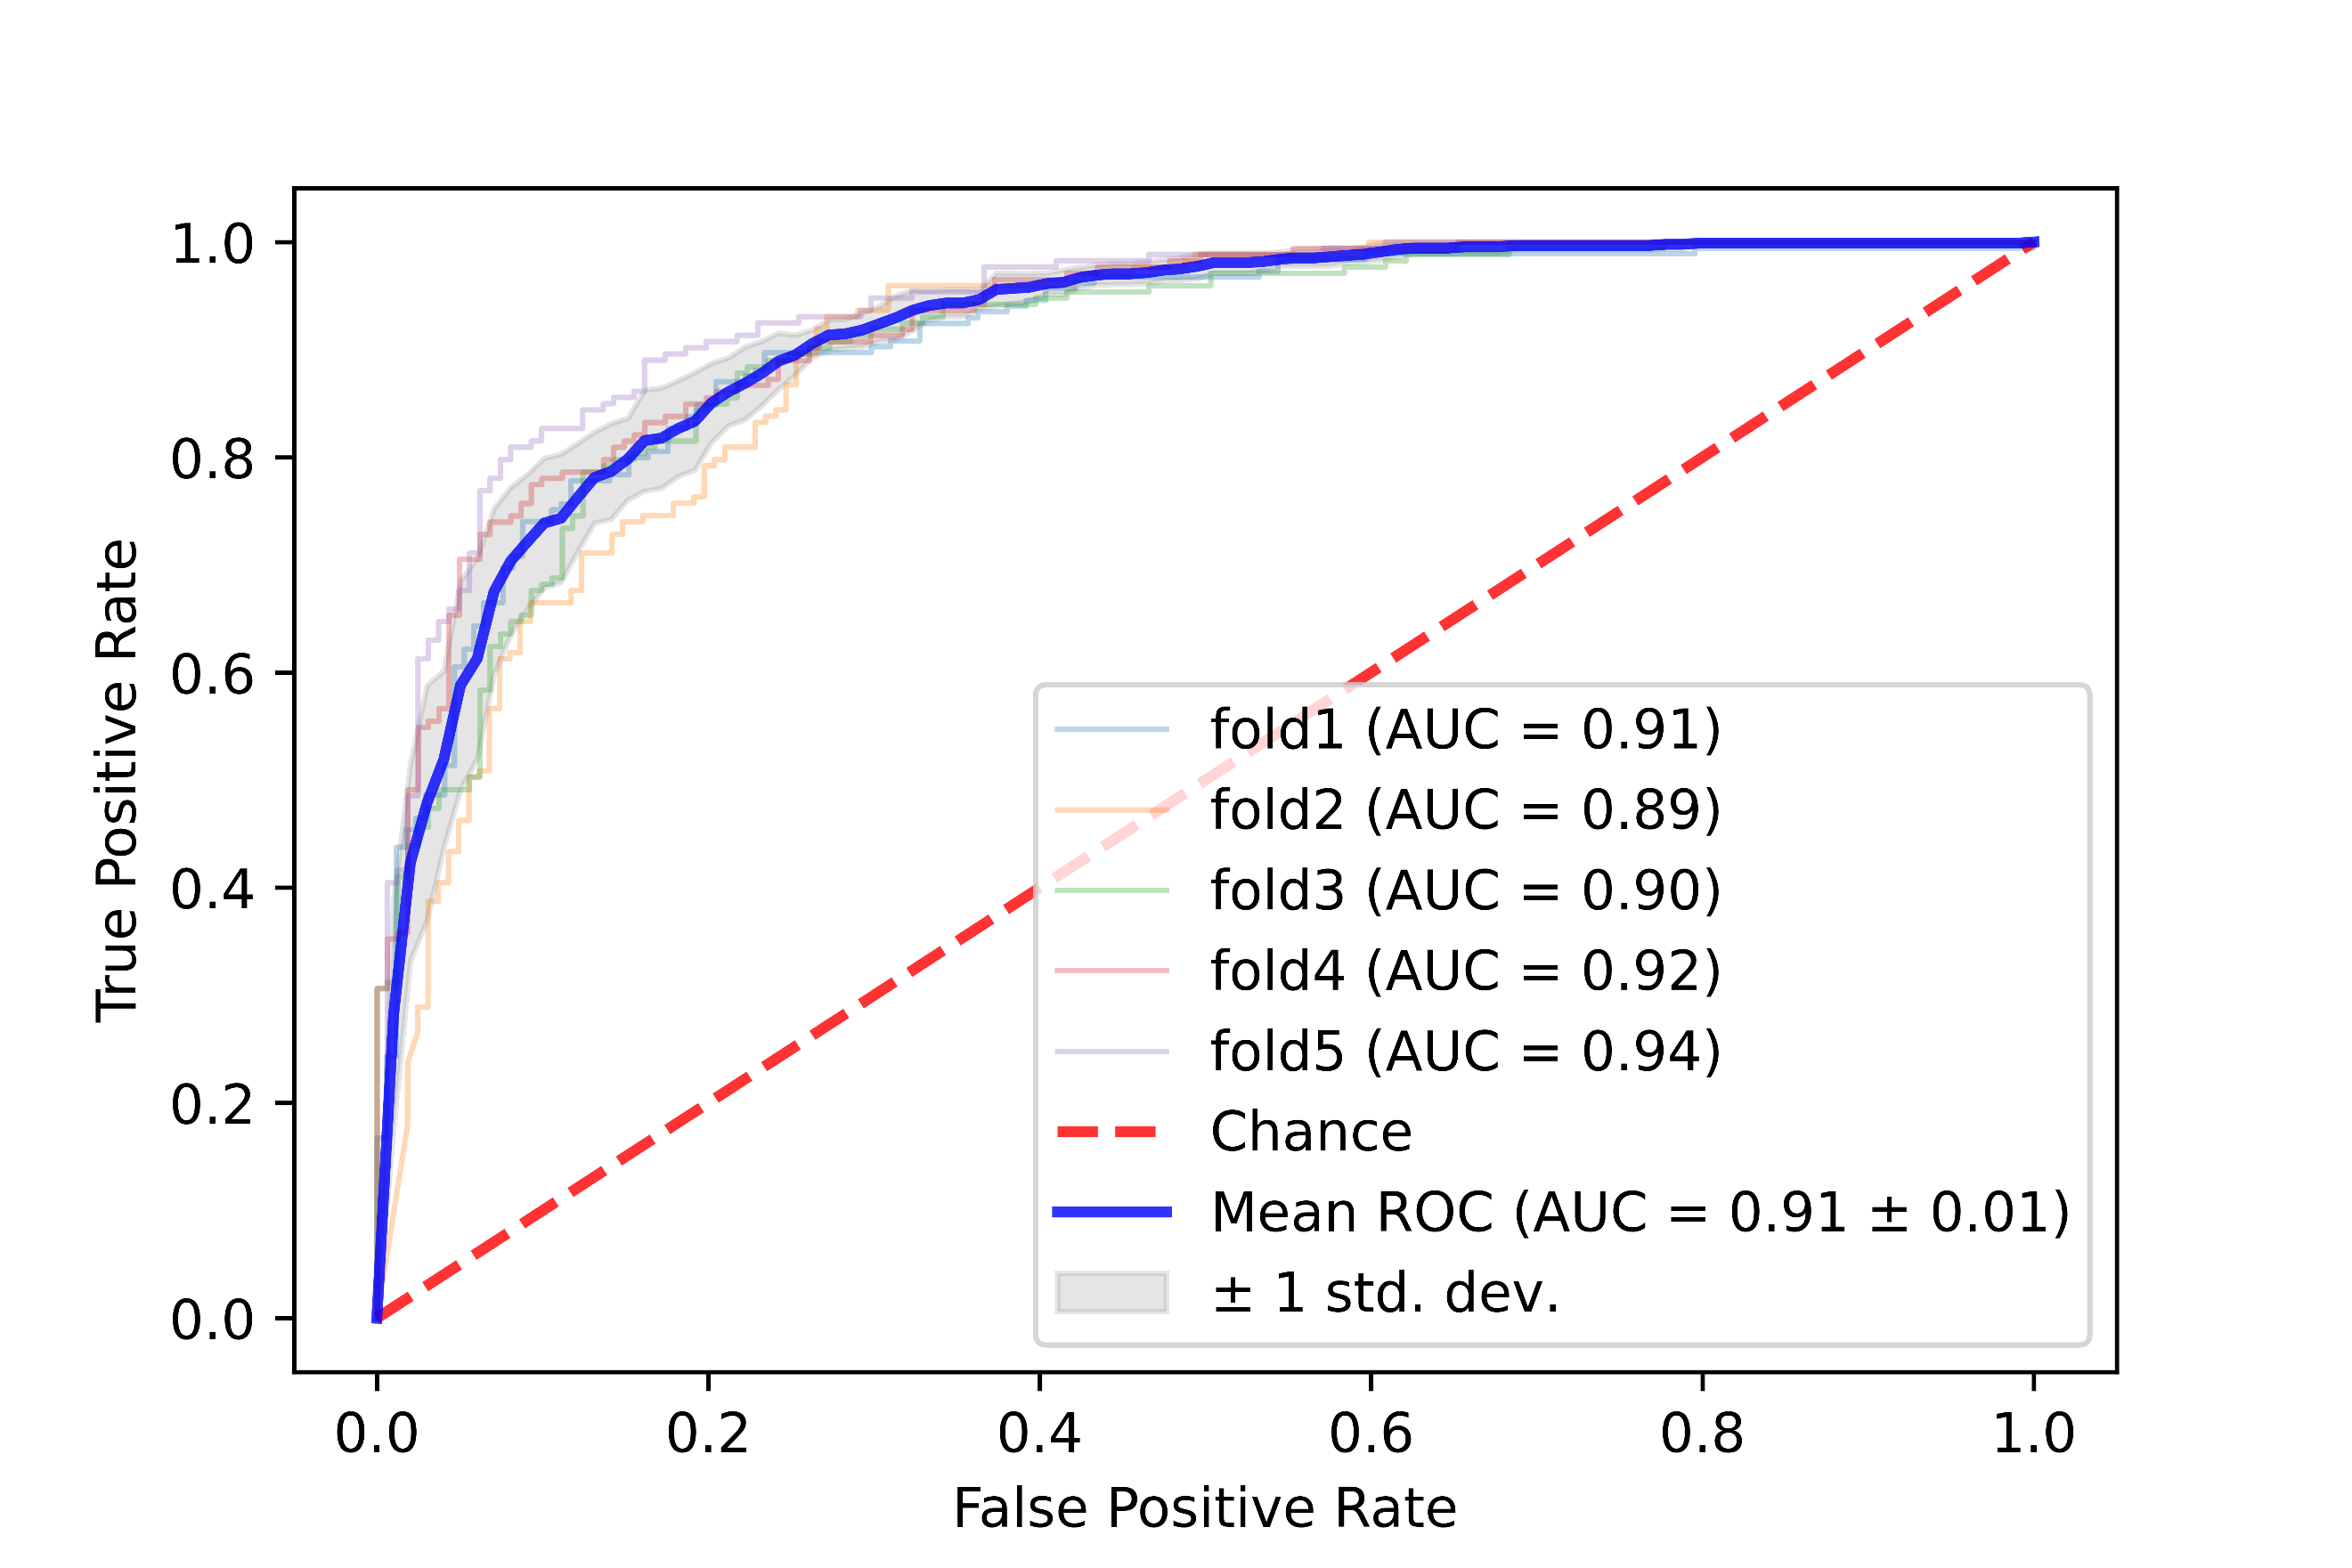
\includegraphics[width=\textwidth,keepaspectratio]{images/Supplement4/image90.png}
		\caption{ROC curve.}
	\end{subfigure}
	\hfill
	\begin{subfigure}[b]{0.49\textwidth}
		\centering
		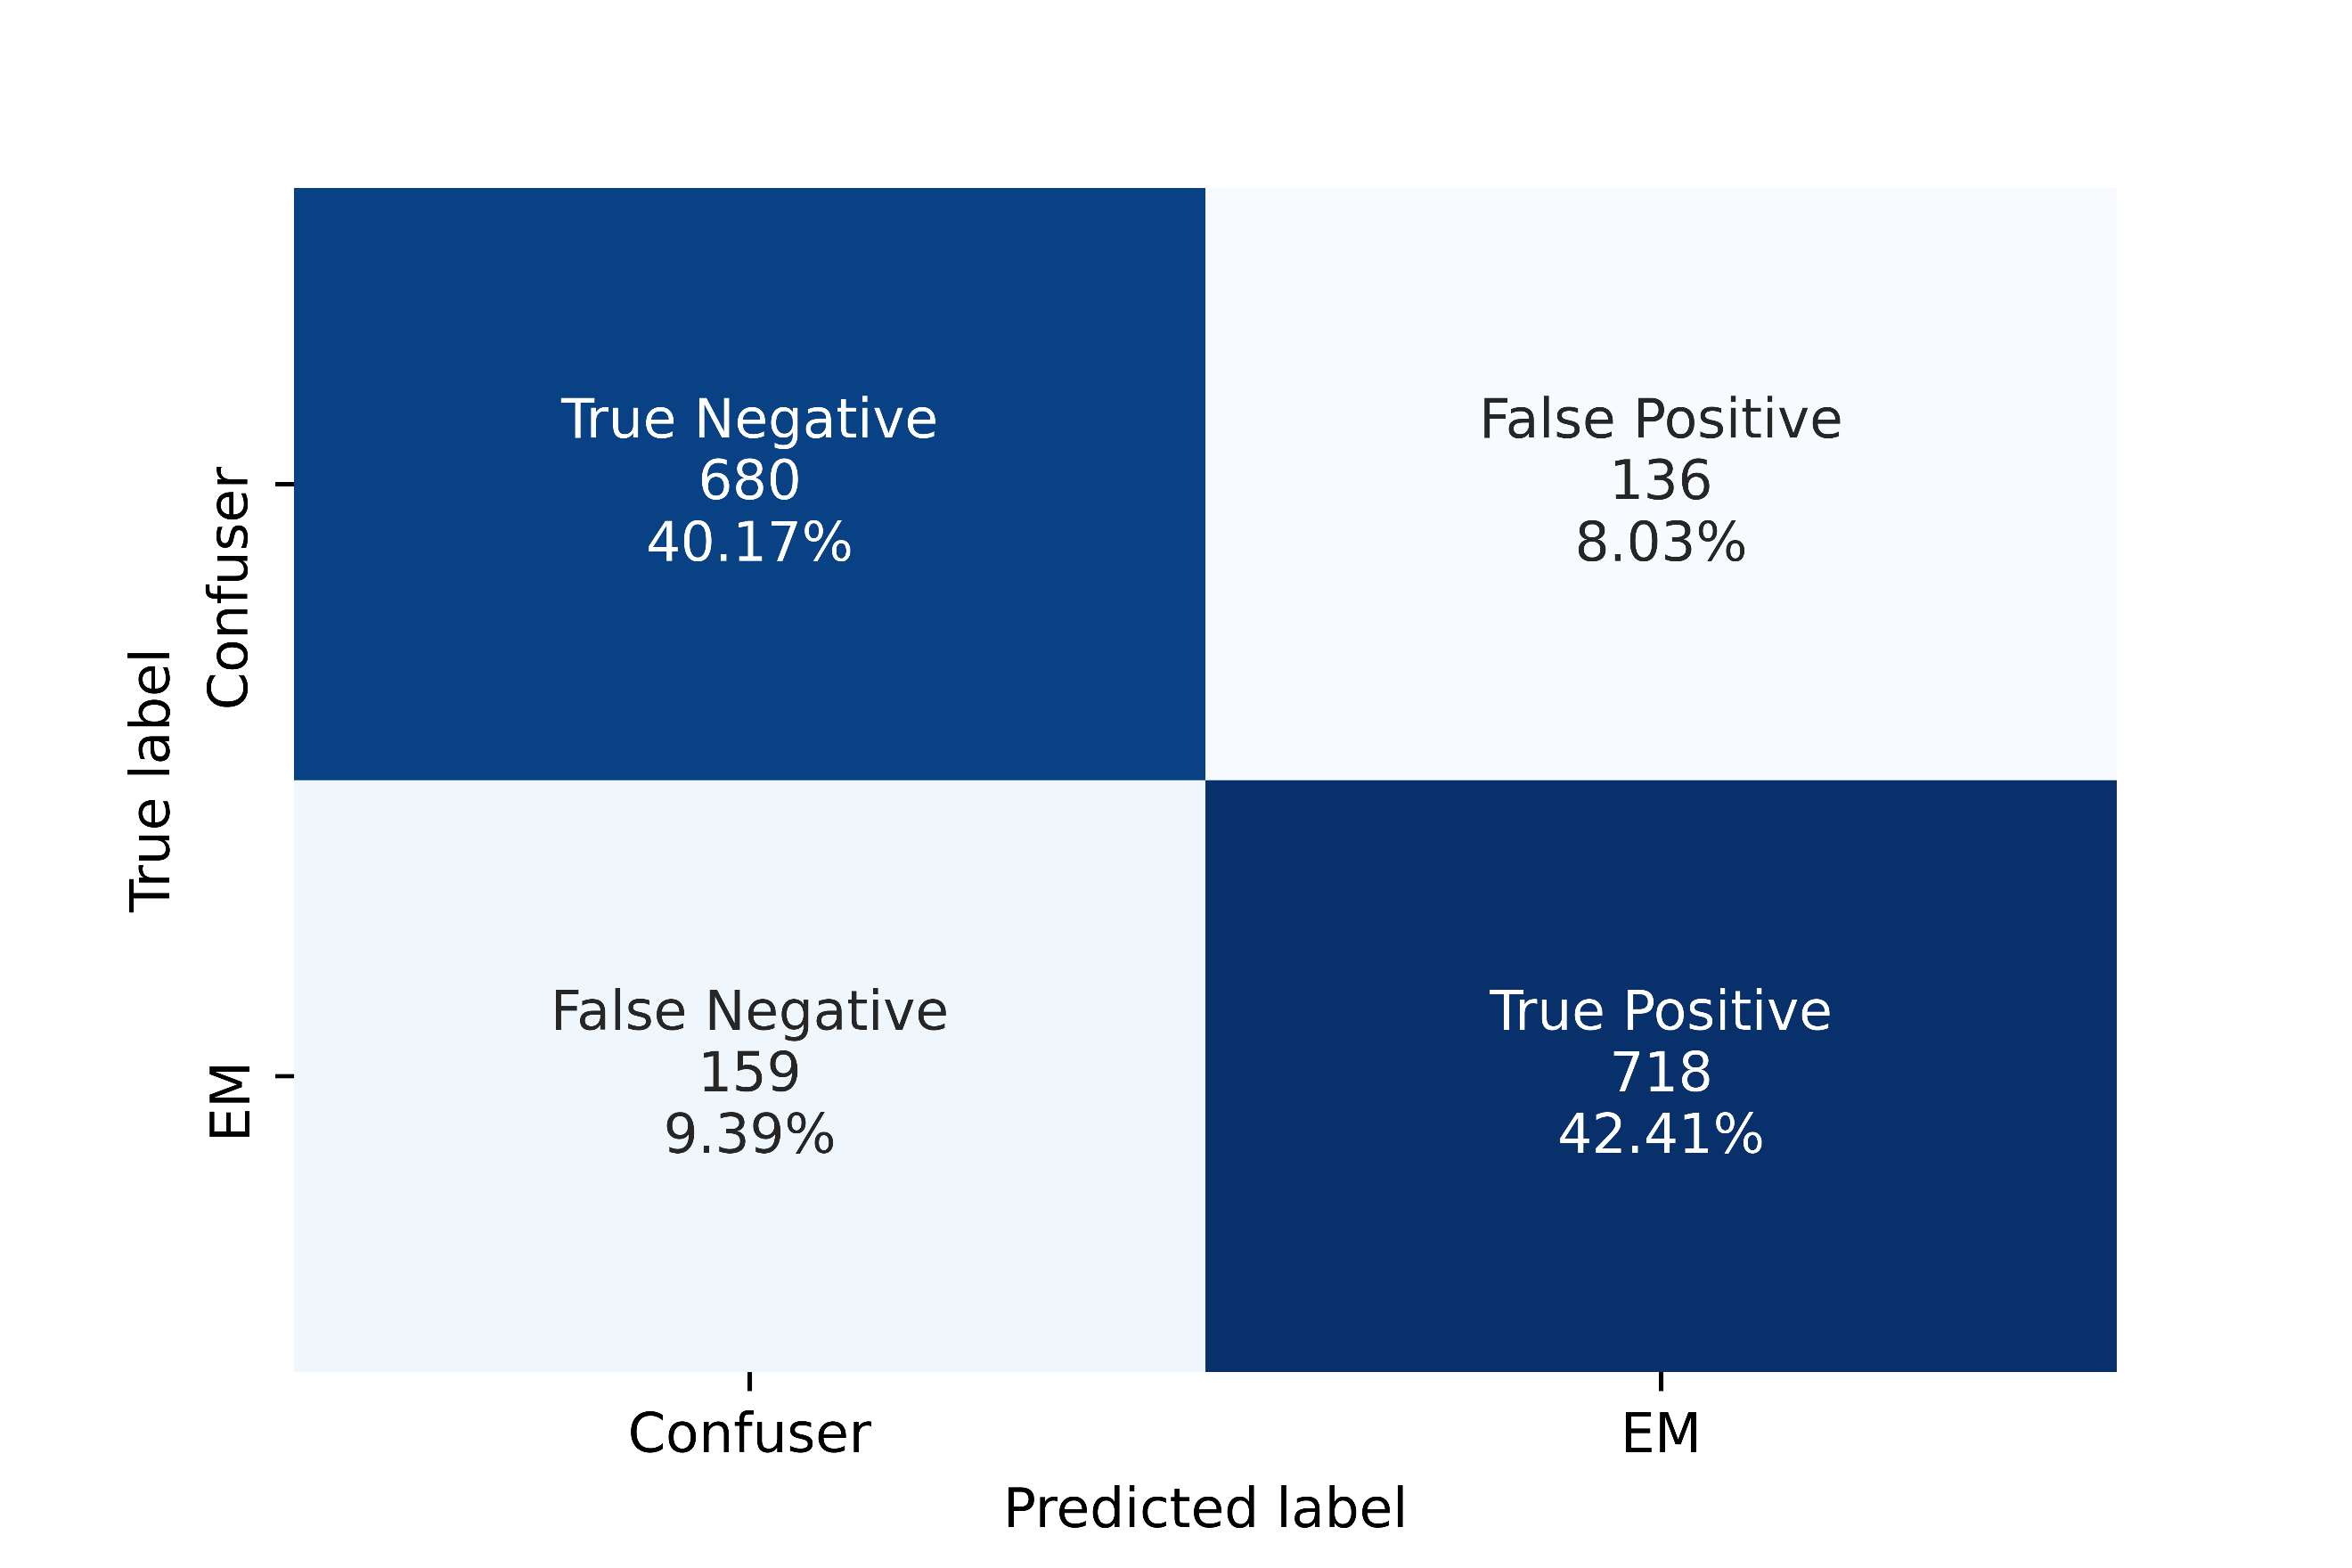
\includegraphics[width=\textwidth,keepaspectratio]{images/Supplement4/image96.png}
		\caption{Confusion matrix.}
	\end{subfigure}
	\caption{Five-fold cross-validation ROC curve and confusion matrix of ResNet101V2-233 model.}
\end{figure}

%%%%%%%%%%%%%%Break%%%%%%%%%%%%%%%%%%%%%%
\vfill\clearpage
\subsection{InceptionV3-274}

\begin{table}[h!]
	\centering
	\caption{Five-fold cross-validation performance metrics of InceptionV3-274 model.}
	\resizebox{\textwidth}{!}{%
		\begin{tabular}{llllllllllll}
			\toprule
			& \multicolumn{11}{c}{\textbf{Metric}}    \\ \cmidrule(lr){2-12} 
			\multicolumn{1}{l}{\textbf{Fold}} & \rotatebox{45}{Accuracy} & 
			\rotatebox{45}{Sensitivity} & \rotatebox{45}{Specificity} & 
			\rotatebox{45}{Precision} & \rotatebox{45}{NPV} & \rotatebox{45}{MCC} & 
			\rotatebox{45}{Kappa} & \rotatebox{45}{LR$+$} & \rotatebox{45}{LR$-$} & 
			\rotatebox{45}{F1-Score} & \rotatebox{45}{AUC}  \\ \midrule
			fold1          & 80.06 & 84.86 & 74.85 & 78.5  & 82.05 & 0.6013 & 0.5992 & 3.3749 & 0.2022 & 0.8156 & 0.875  \\
			fold2          & 81.49 & 83.24 & 79.63 & 81.36 & 81.65 & 0.6293 & 0.6292 & 4.0862 & 0.2105 & 0.8229 & 0.8963 \\
			fold3          & 82.34 & 86.13 & 78.26 & 80.98 & 84    & 0.6468 & 0.6454 & 3.9618 & 0.1773 & 0.8347 & 0.907  \\
			fold4          & 83.53 & 89.6  & 77.02 & 80.73 & 87.32 & 0.6733 & 0.6689 & 3.8986 & 0.1351 & 0.8493 & 0.921  \\
			fold5          & 86.23 & 89.02 & 83.23 & 85.08 & 87.58 & 0.7246 & 0.7237 & 5.3081 & 0.132  & 0.8701 & 0.9268 \\\cmidrule(lr){1-12}
			average        & 82.73 & 86.57 & 78.6  & 81.33 & 84.52 & 0.6551 & 0.6533 & 4.1259 & 0.1714 & 0.8385 & 0.9052 \\
			std. deviation & 2.08  & 2.42  & 2.8   & 2.12  & 2.52  & 0.0419 & 0.0419 & 0.639  & 0.0328 & 0.0195 & 0.0185\\
			\bottomrule
		\end{tabular}%
	}
\end{table}


\begin{figure}[h!]
	\centering
	\begin{subfigure}[b]{0.49\textwidth}
		\centering
		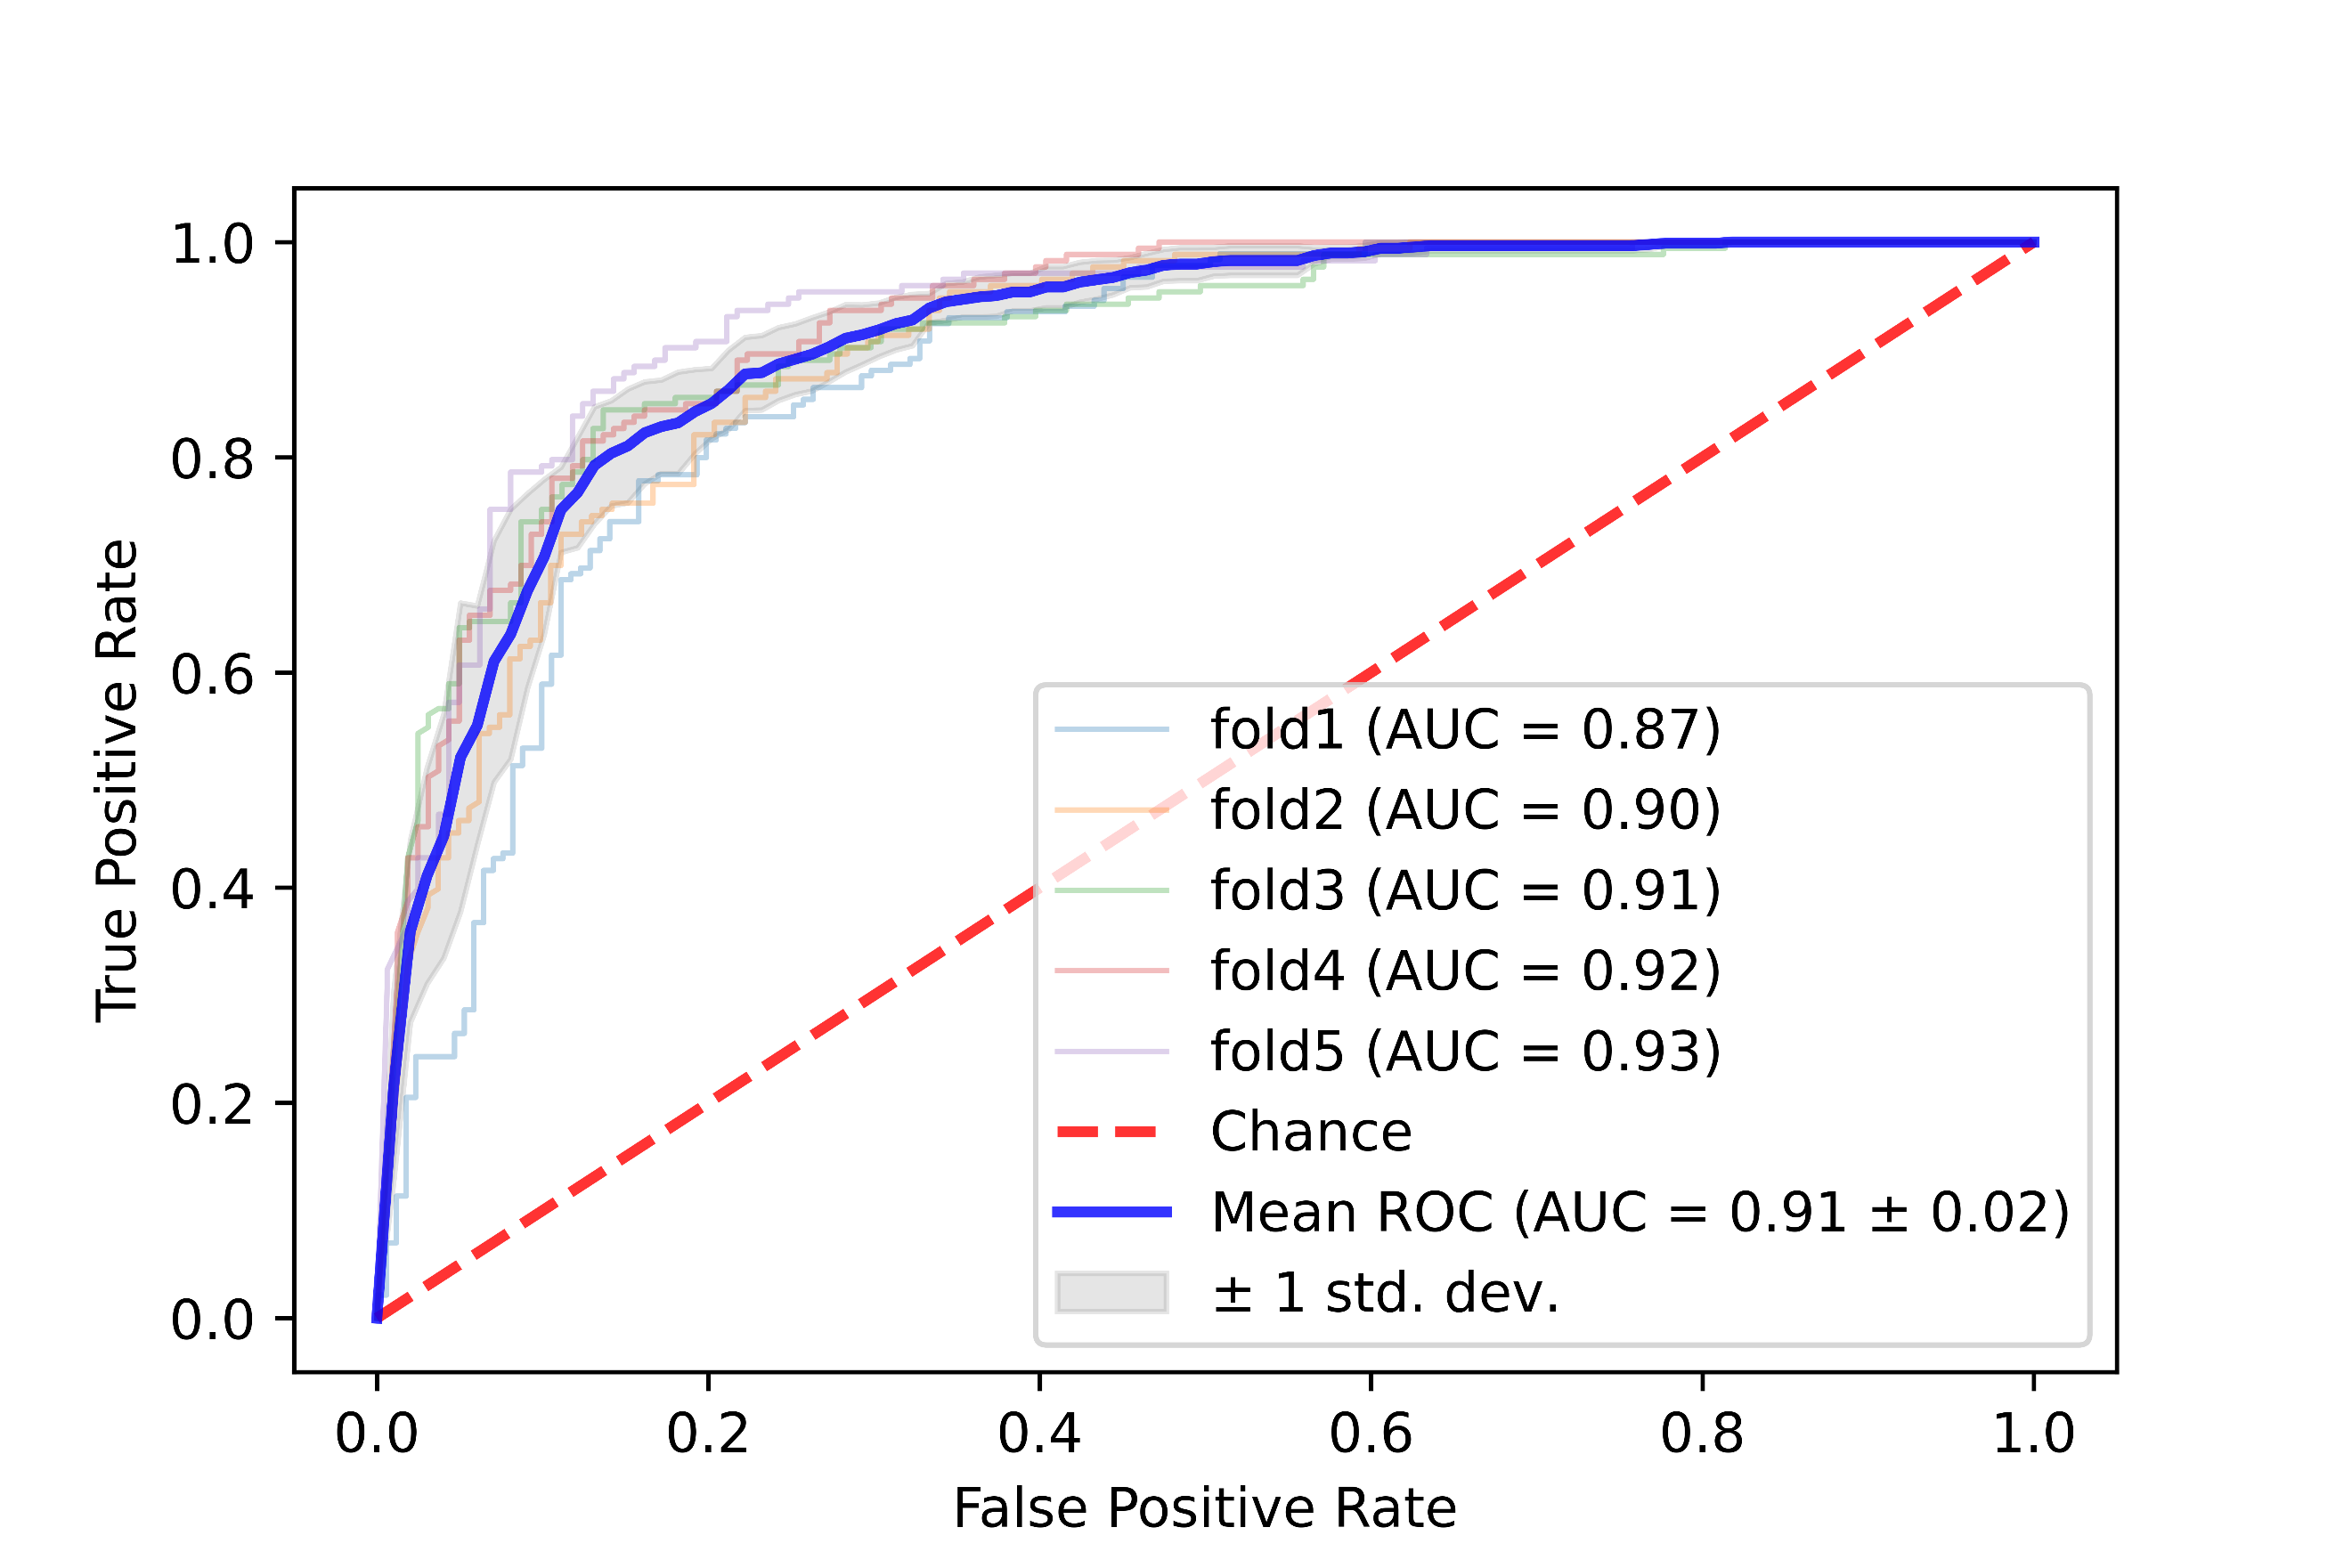
\includegraphics[width=\textwidth,keepaspectratio]{images/Supplement4/image97.png}
		\caption{ROC curve.}
	\end{subfigure}
	\hfill
	\begin{subfigure}[b]{0.49\textwidth}
		\centering
		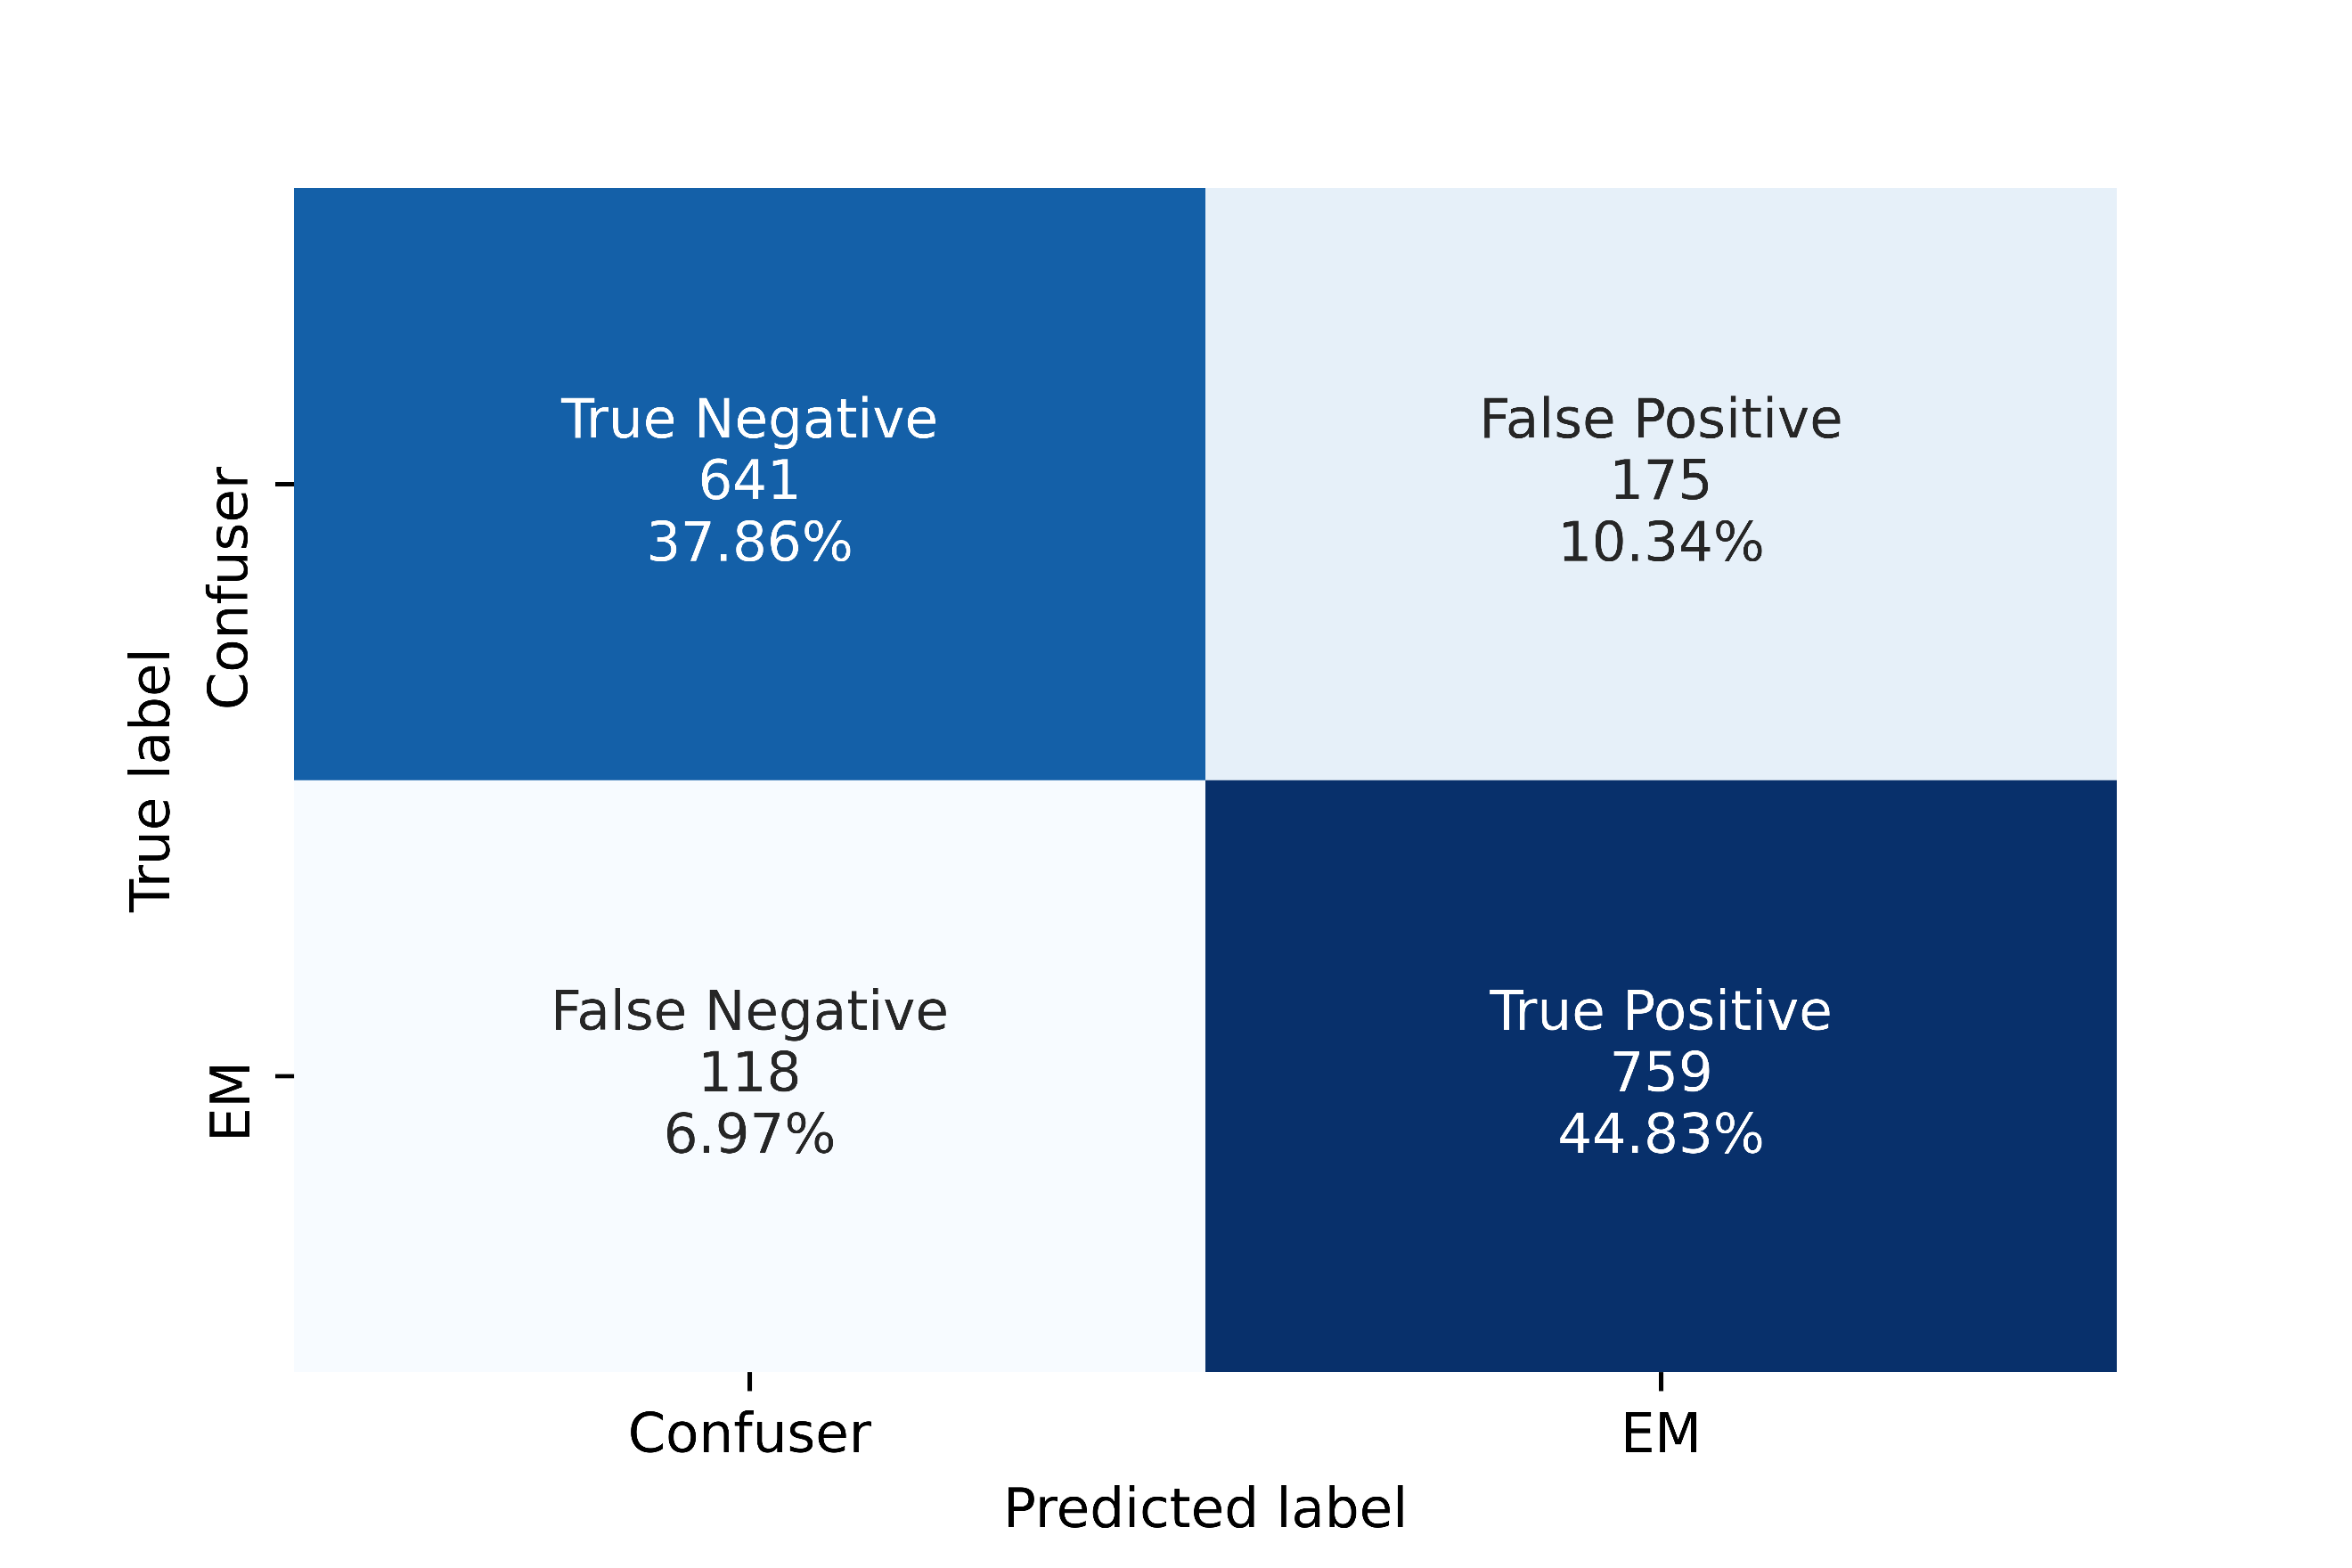
\includegraphics[width=\textwidth,keepaspectratio]{images/Supplement4/image102.png}
		\caption{Confusion matrix.}
	\end{subfigure}
	\caption{Five-fold cross-validation ROC curve and confusion matrix of InceptionV3-102 model.}
\end{figure}

%%%%%%%%%%%%%%Break%%%%%%%%%%%%%%%%%%%%%%
\vfill\clearpage
\subsection{InceptionV4-327}

\begin{table}[h!]
	\centering
	\caption{Five-fold cross-validation performance metrics of InceptionV4-327 model.}
	\resizebox{\textwidth}{!}{%
		\begin{tabular}{llllllllllll}
			\toprule
			& \multicolumn{11}{c}{\textbf{Metric}}    \\ \cmidrule(lr){2-12} 
			\multicolumn{1}{l}{\textbf{Fold}} & \rotatebox{45}{Accuracy} & 
			\rotatebox{45}{Sensitivity} & \rotatebox{45}{Specificity} & 
			\rotatebox{45}{Precision} & \rotatebox{45}{NPV} & \rotatebox{45}{MCC} & 
			\rotatebox{45}{Kappa} & \rotatebox{45}{LR$+$} & \rotatebox{45}{LR$-$} & 
			\rotatebox{45}{F1-Score} & \rotatebox{45}{AUC}  \\ \midrule
			fold1          & 82.58 & 89.19 & 75.44 & 79.71 & 86.58 & 0.6545 & 0.6494 & 3.6313 & 0.1433 & 0.8418 & 0.9074 \\
			fold2          & 80.3  & 79.19 & 81.48 & 82.04 & 78.57 & 0.6064 & 0.606  & 4.2763 & 0.2554 & 0.8059 & 0.8907 \\
			fold3          & 81.44 & 83.82 & 78.88 & 81.01 & 81.94 & 0.6282 & 0.6278 & 3.9689 & 0.2052 & 0.8239 & 0.8884 \\
			fold4          & 85.03 & 86.13 & 83.85 & 85.14 & 84.91 & 0.7001 & 0.7001 & 5.3333 & 0.1654 & 0.8563 & 0.9393 \\
			fold5          & 84.43 & 90.17 & 78.26 & 81.68 & 88.11 & 0.6911 & 0.687  & 4.148  & 0.1256 & 0.8571 & 0.9202 \\\cmidrule(lr){1-12}
			average        & 82.76 & 85.7  & 79.58 & 81.92 & 84.02 & 0.6561 & 0.6541 & 4.2716 & 0.179  & 0.837  & 0.9092 \\
			std. deviation & 1.78  & 3.96  & 2.87  & 1.8   & 3.41  & 0.0358 & 0.0353 & 0.5734 & 0.0465 & 0.0197 & 0.019 \\
			\bottomrule
		\end{tabular}%
	}
\end{table}


\begin{figure}[h!]
	\centering
	\begin{subfigure}[b]{0.49\textwidth}
		\centering
		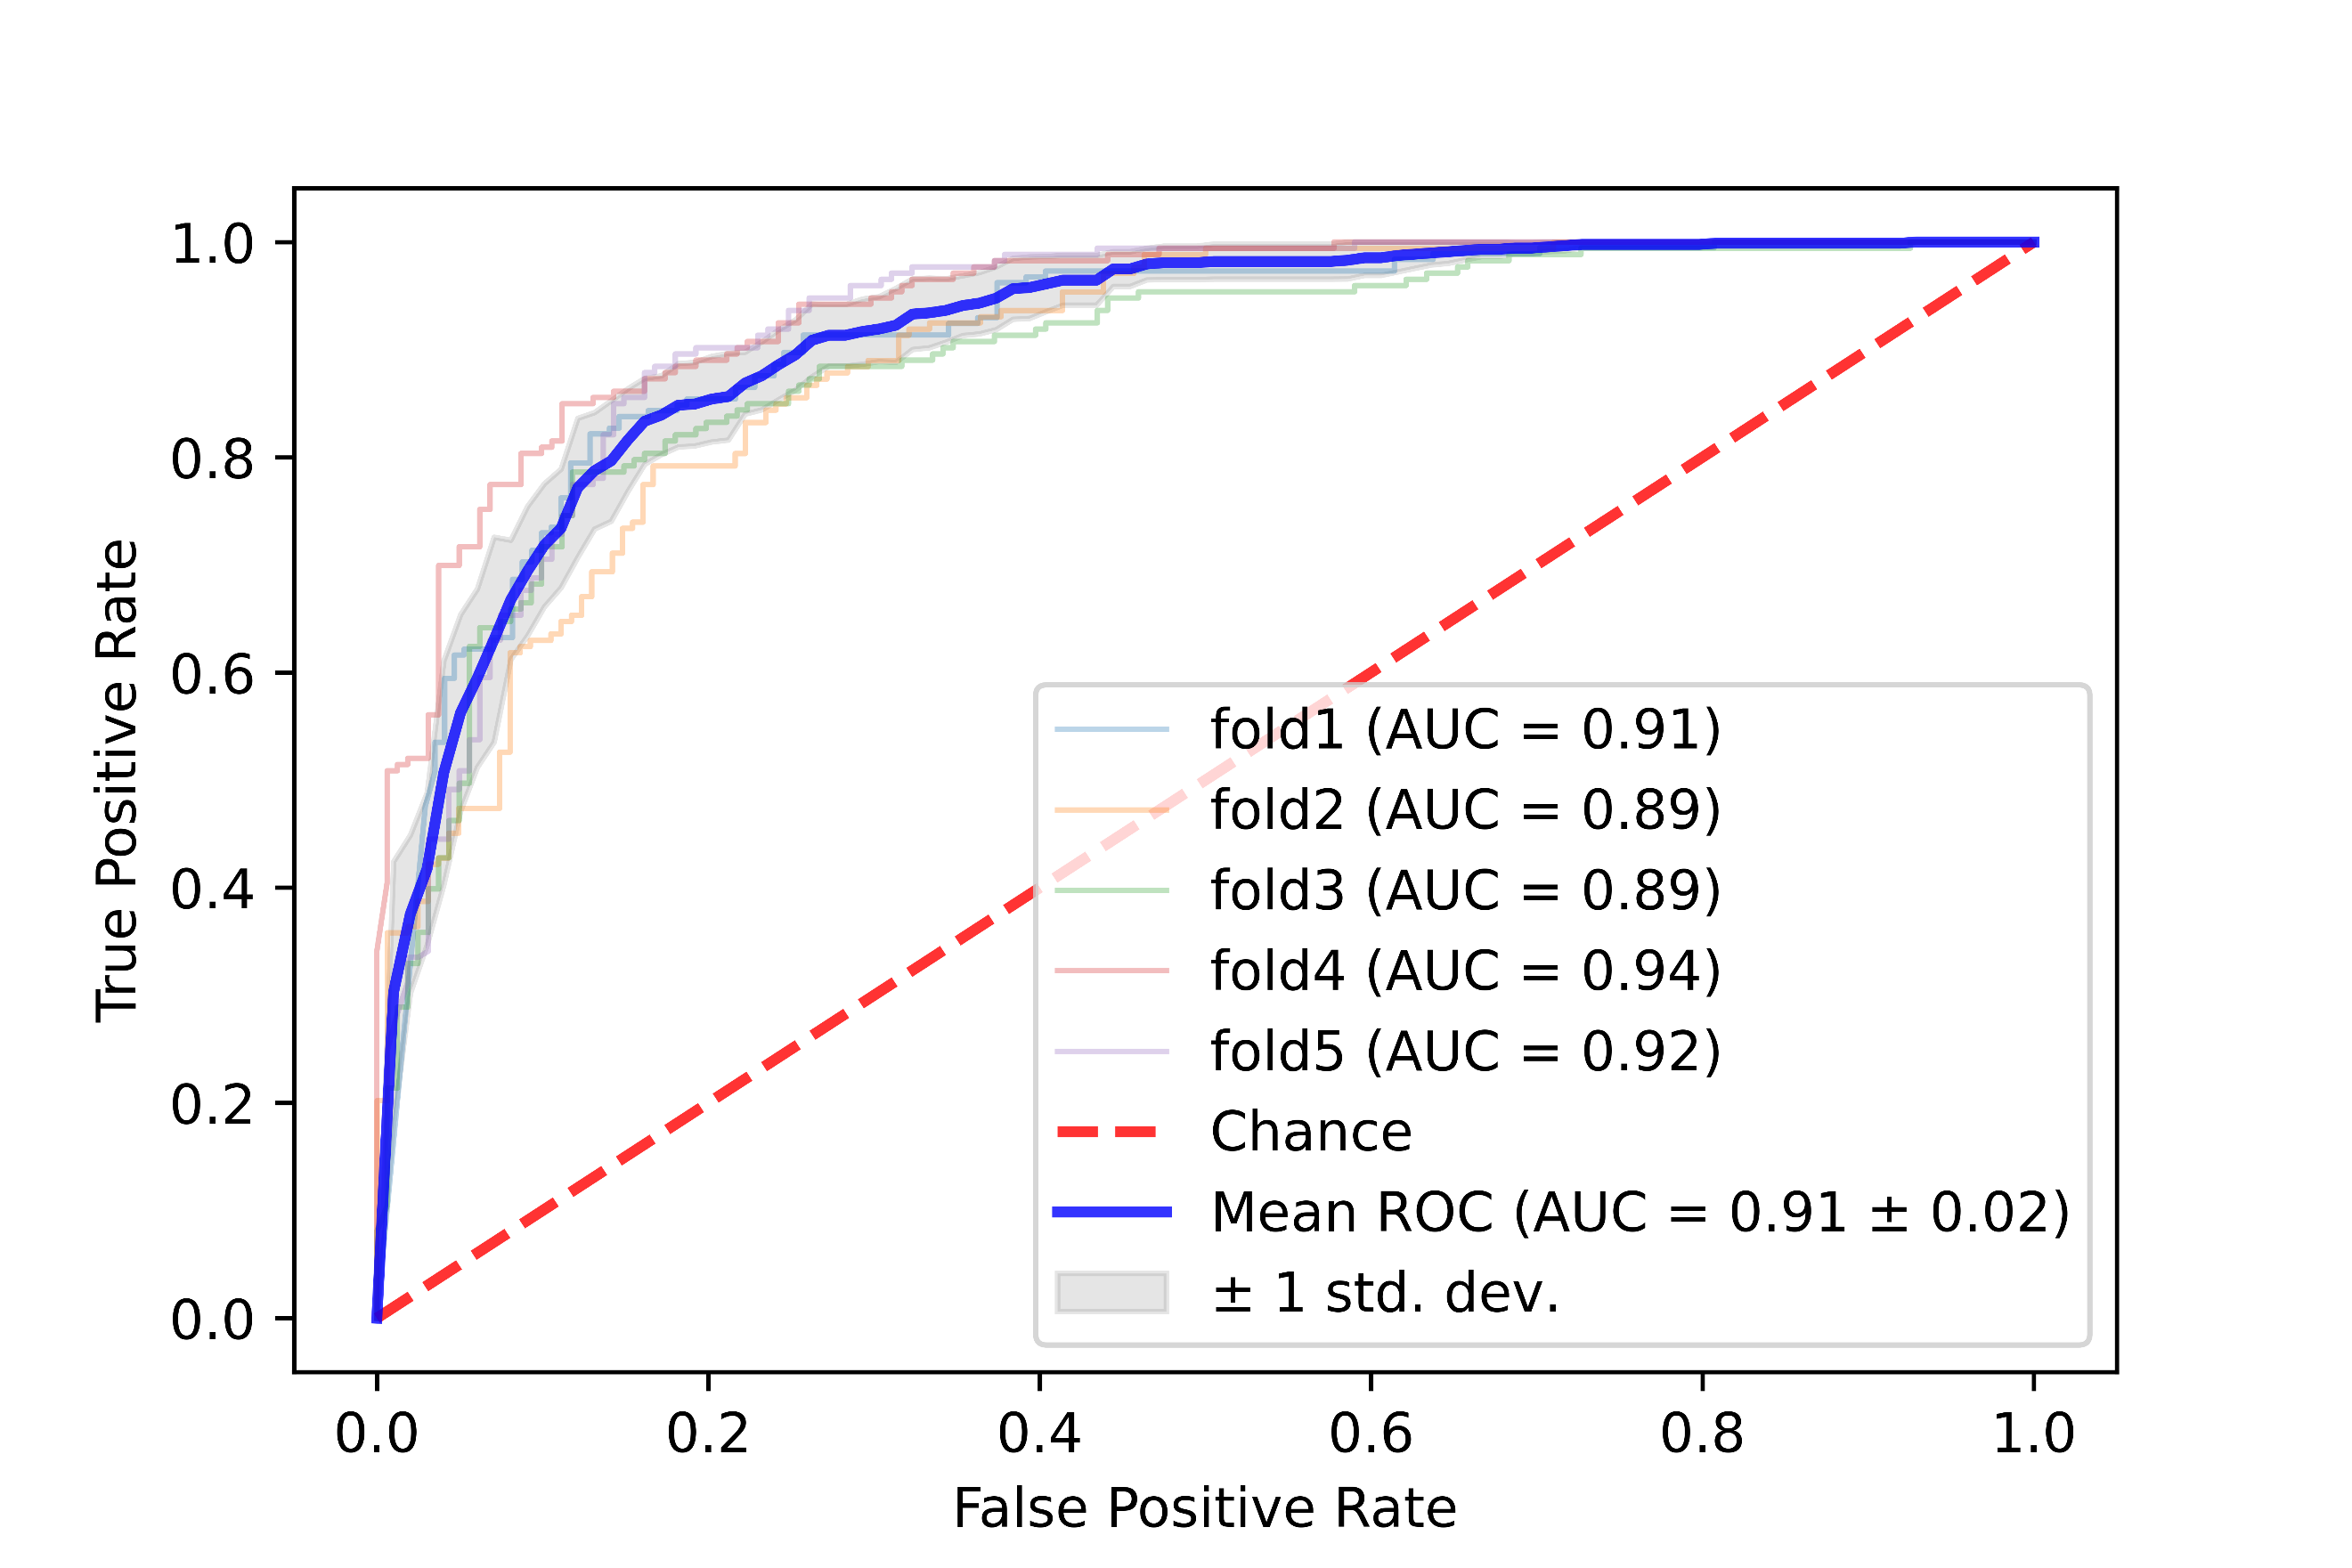
\includegraphics[width=\textwidth,keepaspectratio]{images/Supplement4/image103.png}
		\caption{ROC curve.}
	\end{subfigure}
	\hfill
	\begin{subfigure}[b]{0.49\textwidth}
		\centering
		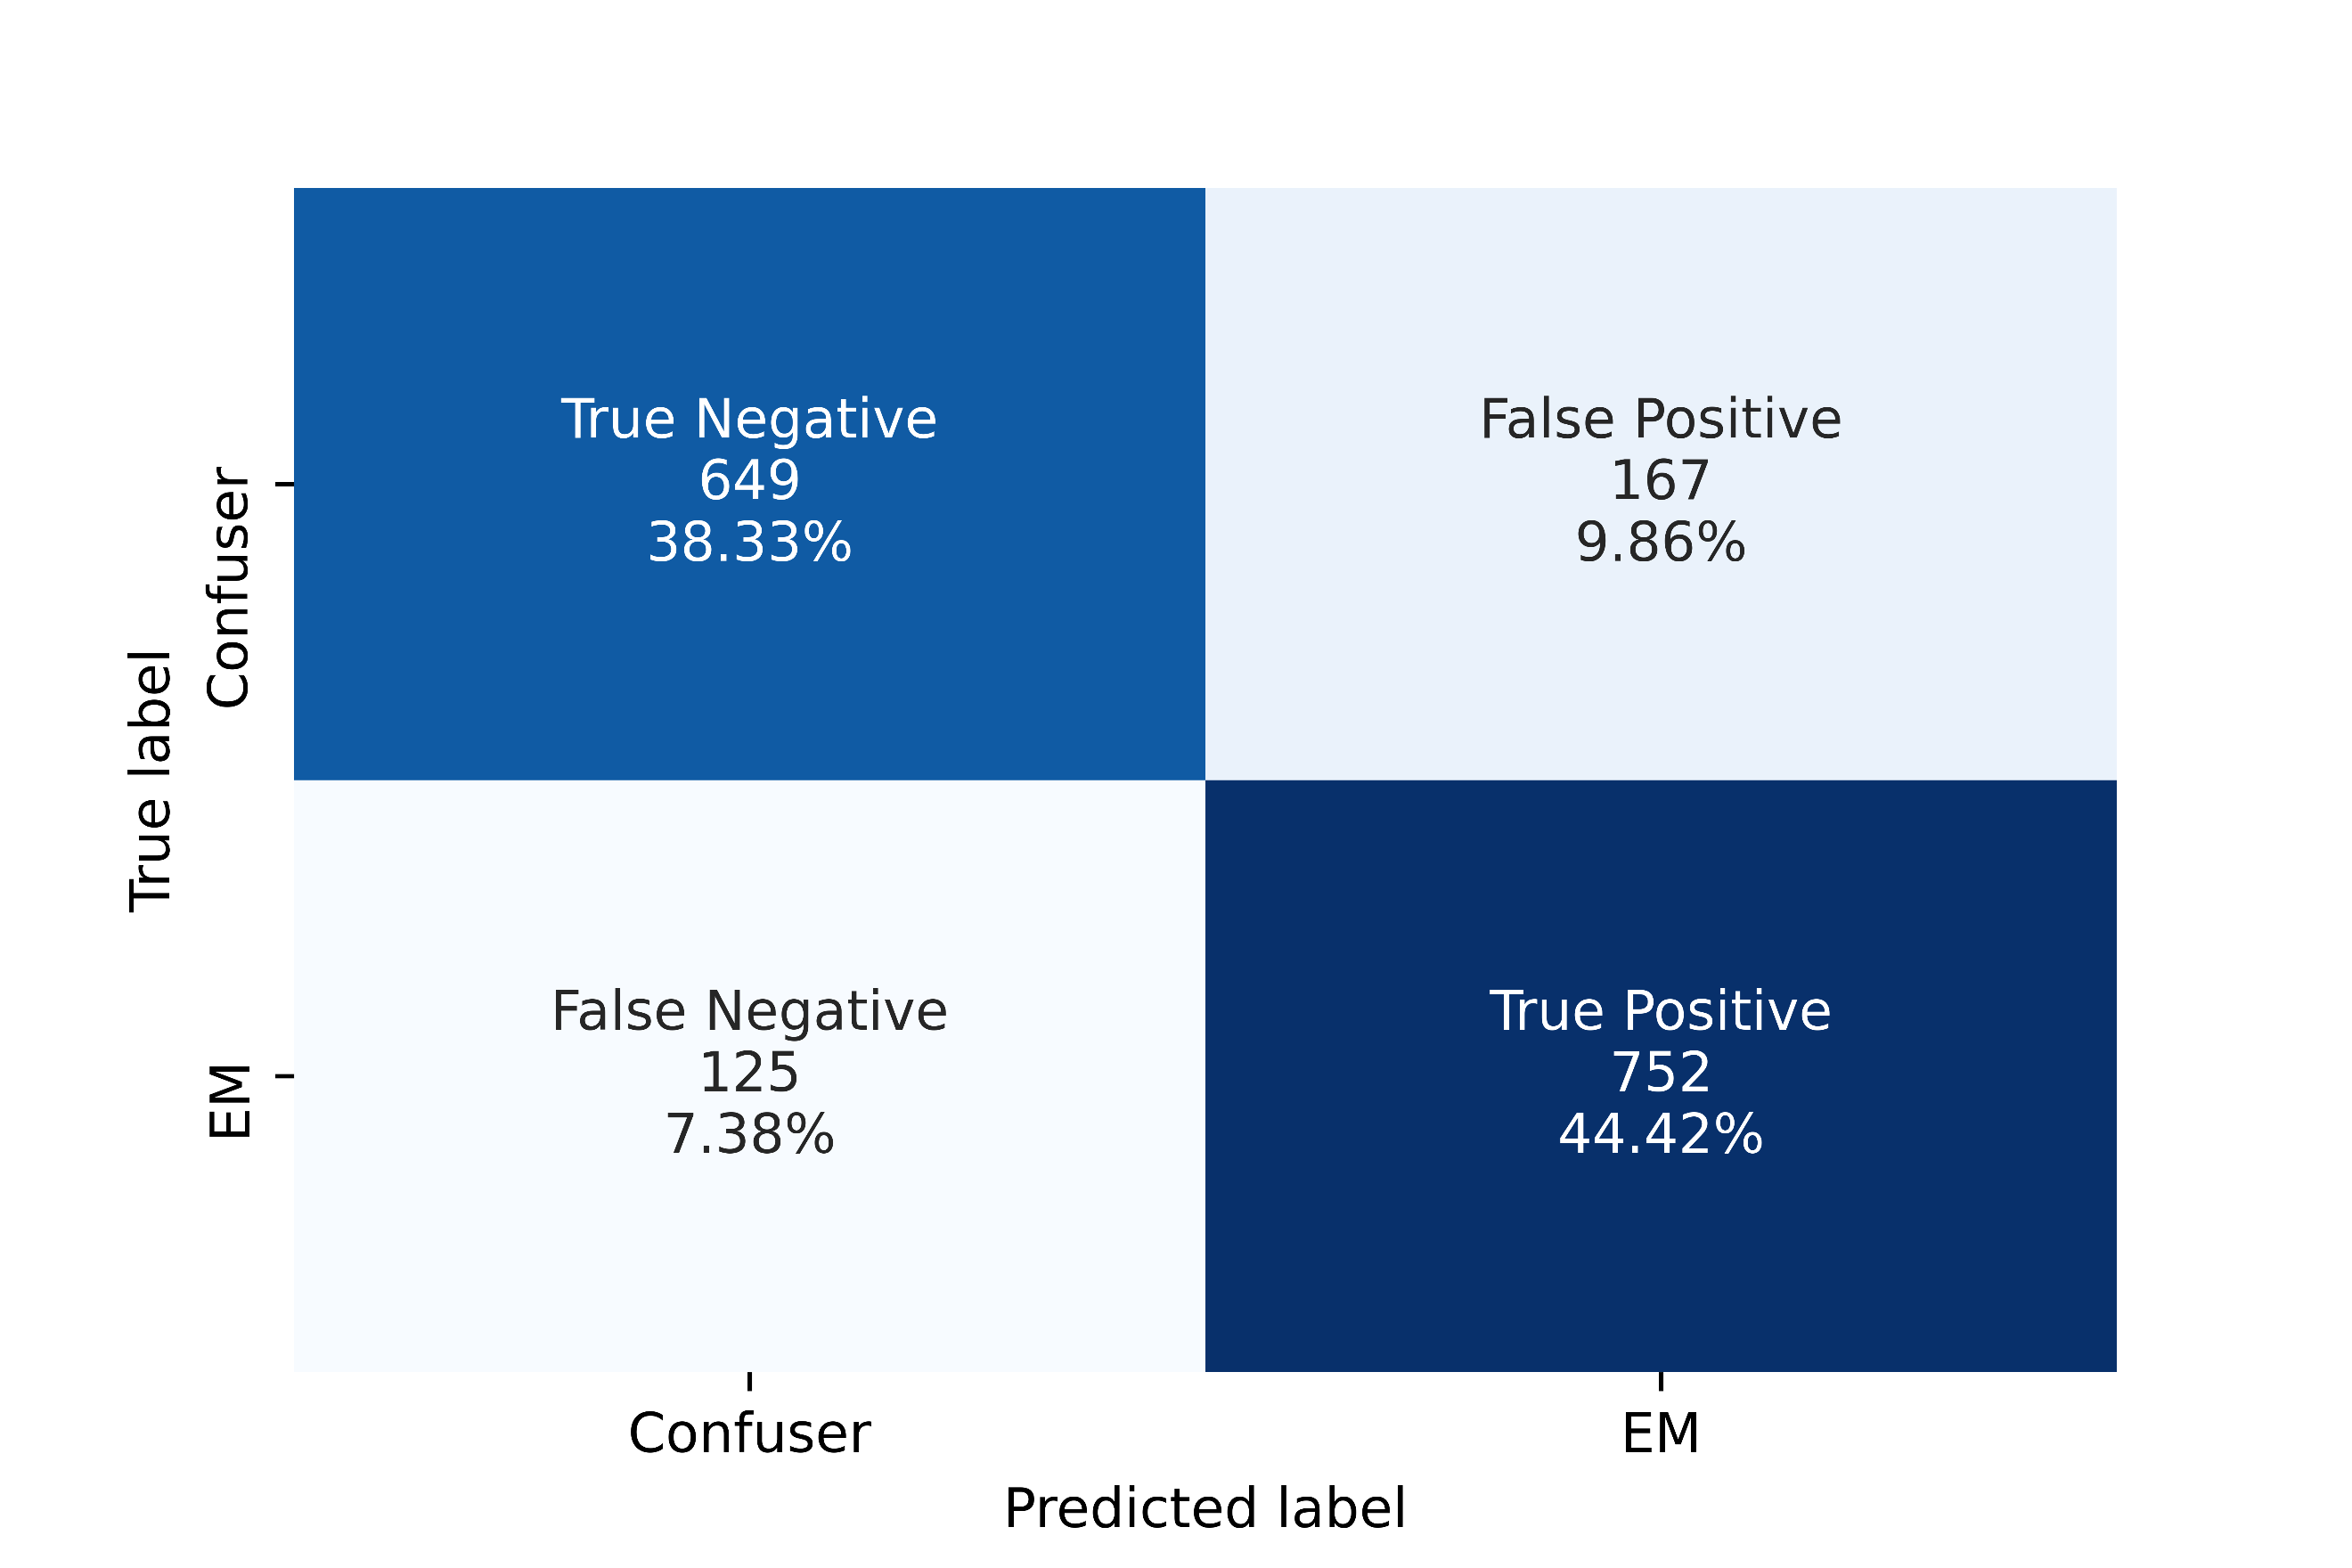
\includegraphics[width=\textwidth,keepaspectratio]{images/Supplement4/image109.png}
		\caption{Confusion matrix.}
	\end{subfigure}
	\caption{Five-fold cross-validation ROC curve and confusion matrix of InceptionV4-327 model.}
\end{figure}

%%%%%%%%%%%%%%Break%%%%%%%%%%%%%%%%%%%%%%
\vfill\clearpage
\subsection{InceptionResNetV2-500}

\begin{table}[h!]
	\centering
	\caption{Five-fold cross-validation performance metrics of InceptionResNetV2-500 model.}
	\resizebox{\textwidth}{!}{%
		\begin{tabular}{llllllllllll}
			\toprule
			& \multicolumn{11}{c}{\textbf{Metric}}    \\ \cmidrule(lr){2-12} 
			\multicolumn{1}{l}{\textbf{Fold}} & \rotatebox{45}{Accuracy} & 
			\rotatebox{45}{Sensitivity} & \rotatebox{45}{Specificity} & 
			\rotatebox{45}{Precision} & \rotatebox{45}{NPV} & \rotatebox{45}{MCC} & 
			\rotatebox{45}{Kappa} & \rotatebox{45}{LR$+$} & \rotatebox{45}{LR$-$} & 
			\rotatebox{45}{F1-Score} & \rotatebox{45}{AUC}  \\ \midrule
			fold1          & 79.78 & 77.84 & 81.87 & 82.29 & 77.35 & 0.5967 & 0.5958 & 4.2936 & 0.2707 & 0.8    & 0.8868 \\
			fold2          & 82.39 & 81.5  & 83.33 & 83.93 & 80.84 & 0.648  & 0.6477 & 4.8902 & 0.222  & 0.827  & 0.9022 \\
			fold3          & 82.34 & 88.44 & 75.78 & 79.69 & 85.92 & 0.6491 & 0.6448 & 3.651  & 0.1526 & 0.8384 & 0.889  \\
			fold4          & 82.63 & 82.66 & 82.61 & 83.63 & 81.6  & 0.6524 & 0.6524 & 4.7529 & 0.2099 & 0.8314 & 0.9036 \\
			fold5          & 86.23 & 87.28 & 85.09 & 86.29 & 86.16 & 0.7241 & 0.7241 & 5.8553 & 0.1494 & 0.8678 & 0.9241 \\\cmidrule(lr){1-12}
			average        & 82.67 & 83.54 & 81.74 & 83.17 & 82.37 & 0.6541 & 0.653  & 4.6886 & 0.2009 & 0.8329 & 0.9011 \\
			std. deviation & 2.06  & 3.88  & 3.16  & 2.16  & 3.32  & 0.0406 & 0.041  & 0.7264 & 0.0456 & 0.0218 & 0.0133\\
			\bottomrule
		\end{tabular}%
	}
\end{table}


\begin{figure}[h!]
	\centering
	\begin{subfigure}[b]{0.49\textwidth}
		\centering
		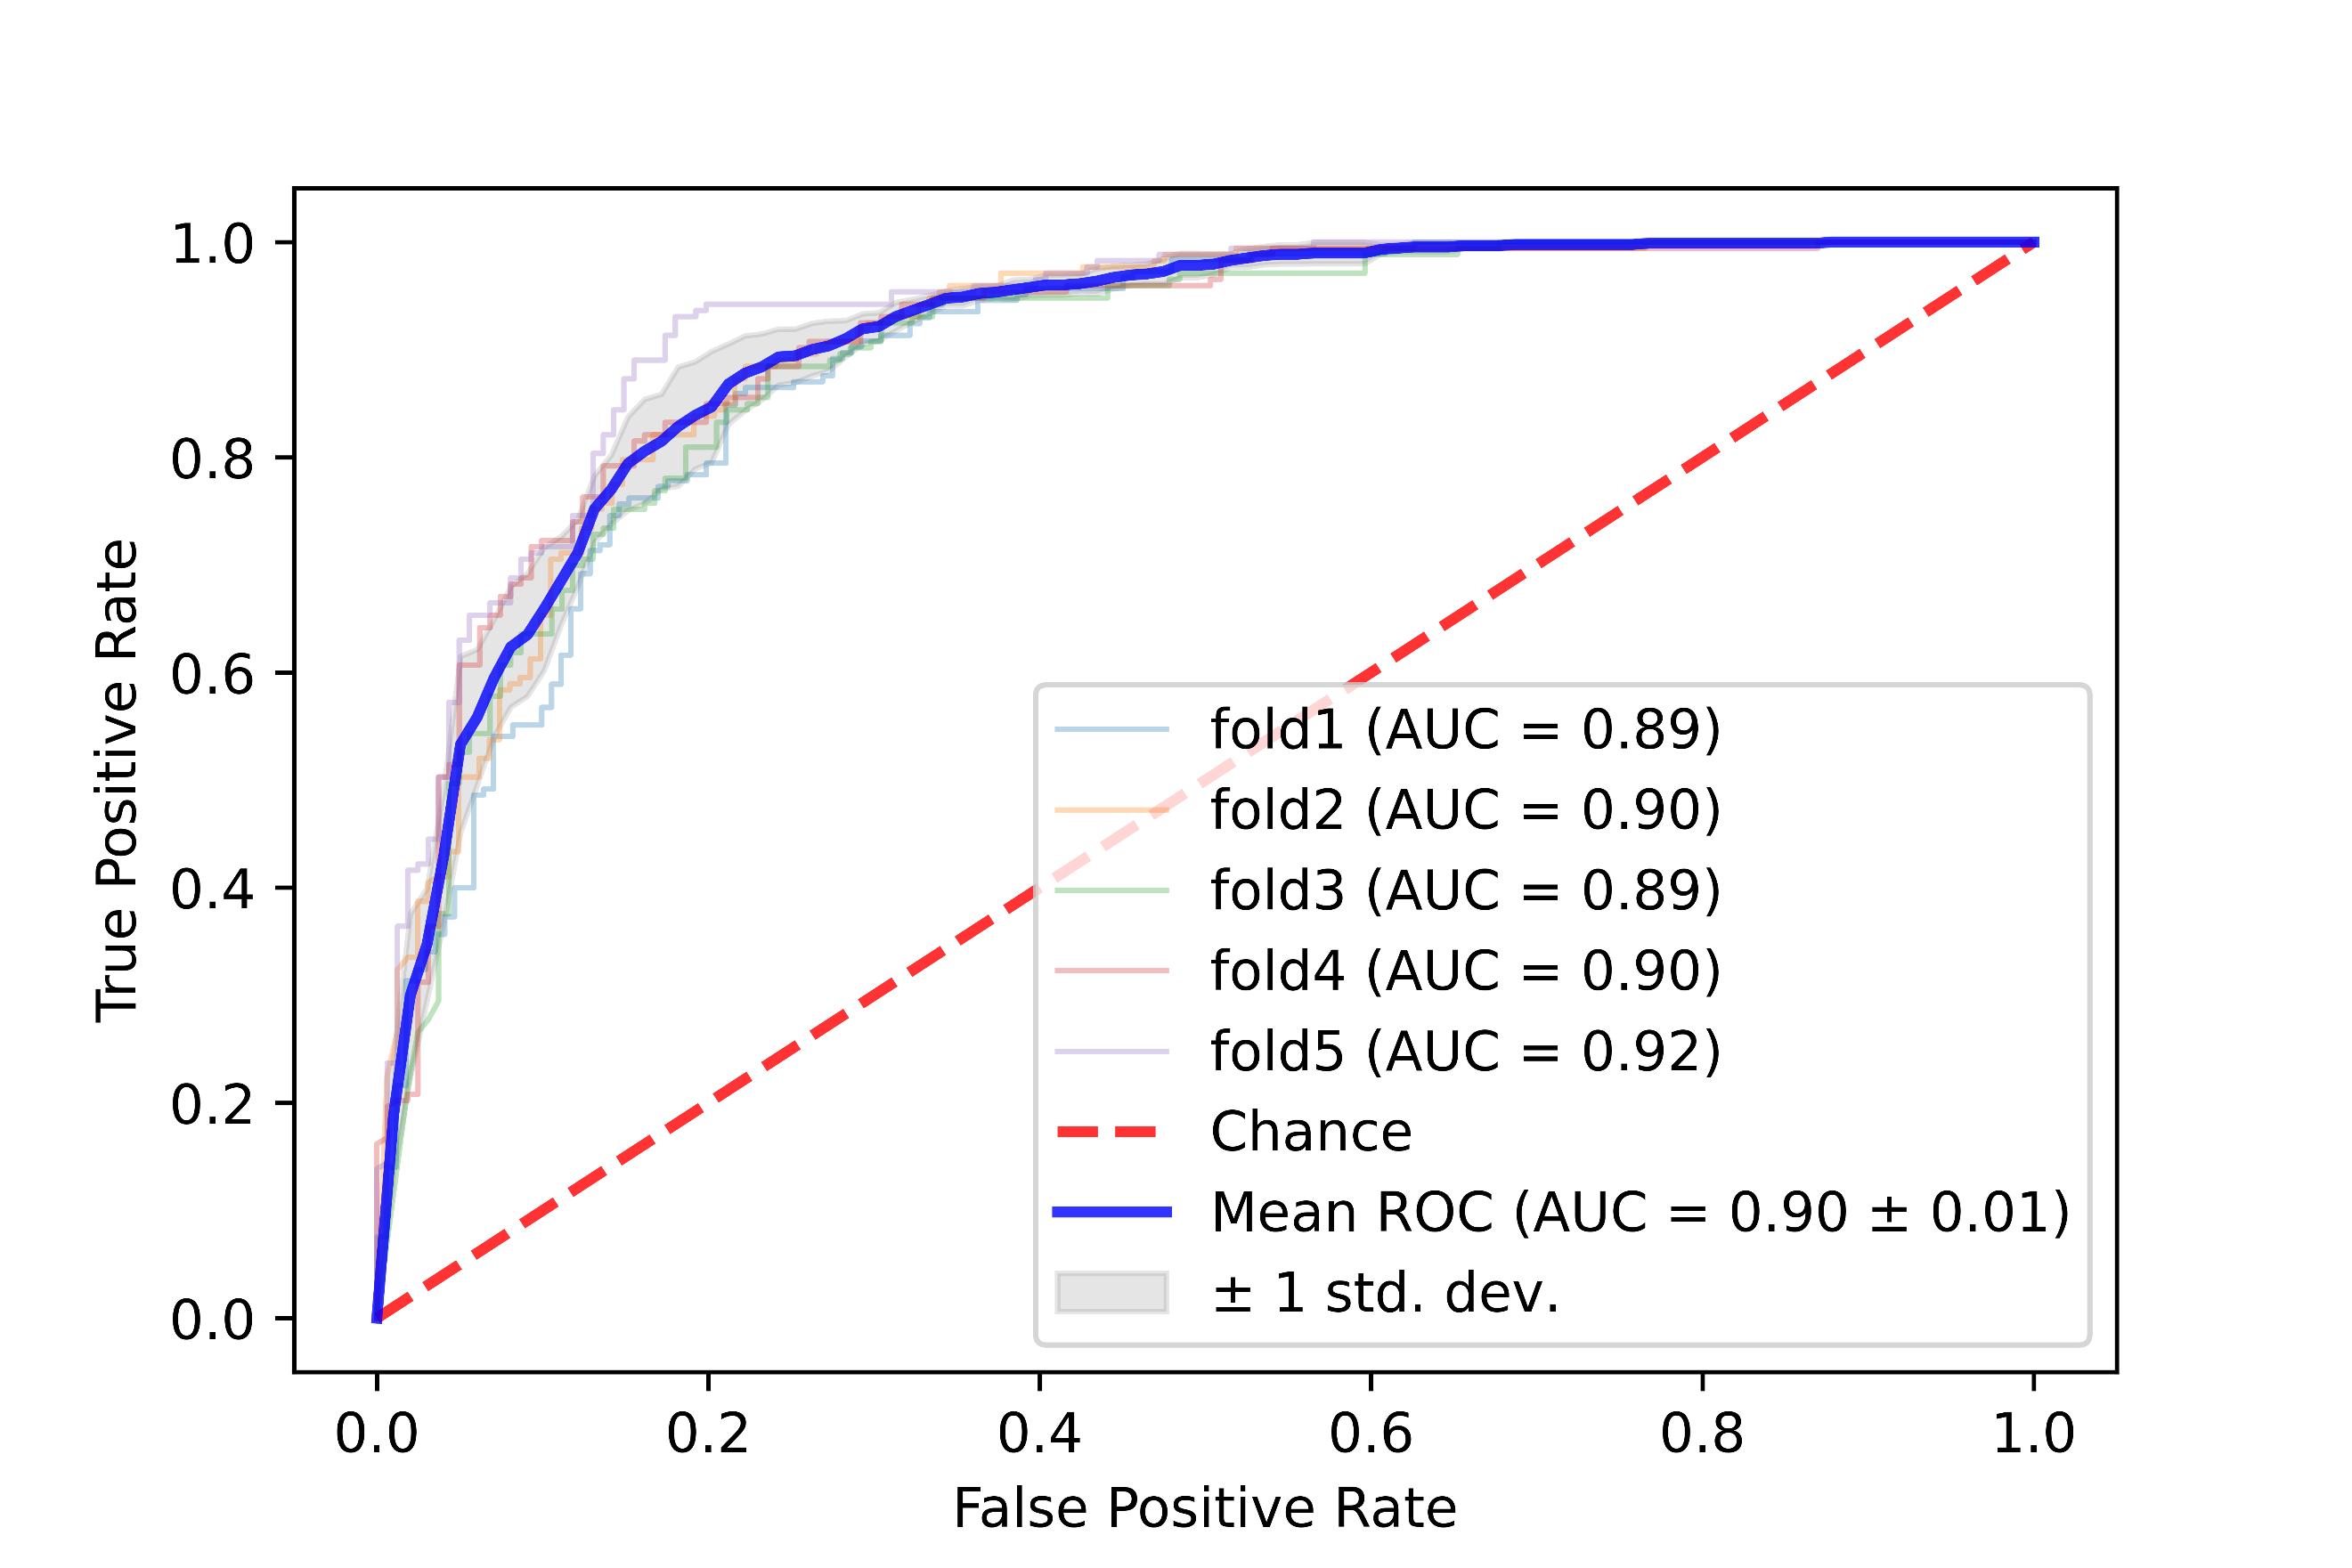
\includegraphics[width=\textwidth,keepaspectratio]{images/Supplement4/image110.png}
		\caption{ROC curve.}
	\end{subfigure}
	\hfill
	\begin{subfigure}[b]{0.49\textwidth}
		\centering
		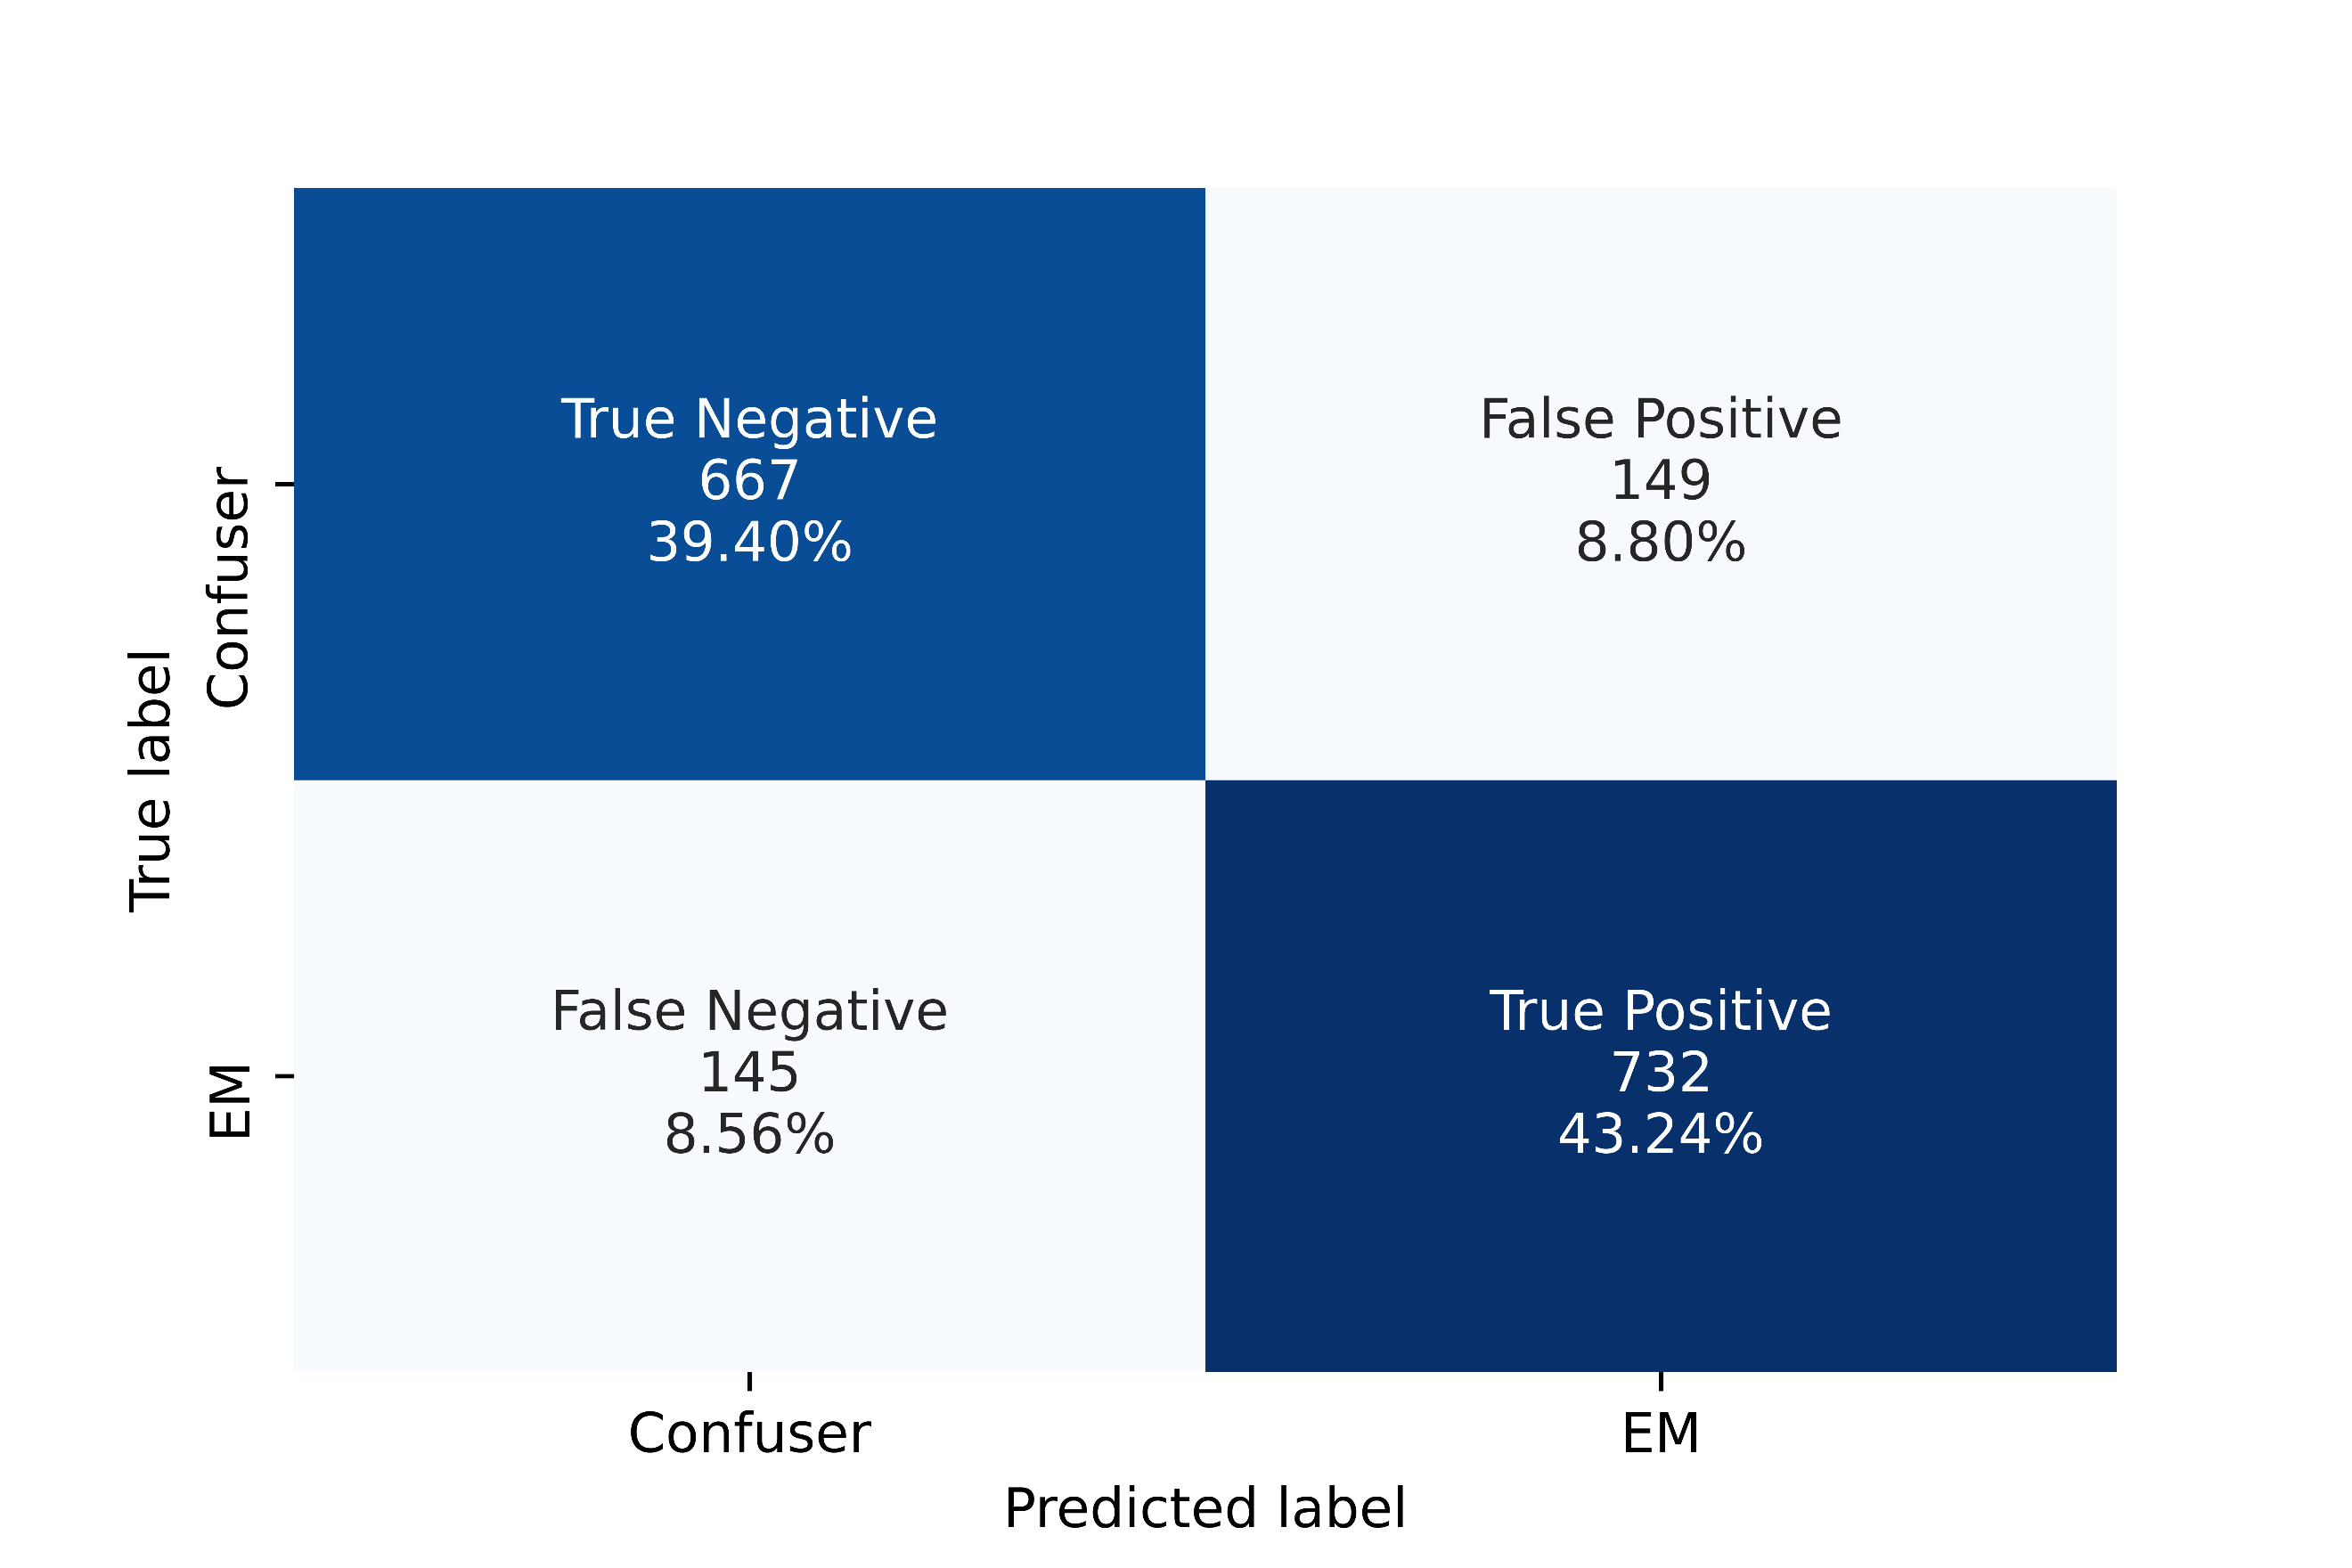
\includegraphics[width=\textwidth,keepaspectratio]{images/Supplement4/image115.png}
		\caption{Confusion matrix.}
	\end{subfigure}
	\caption{Five-fold cross-validation ROC curve and confusion matrix of InceptionResNetV2-500 model.}
\end{figure}

%%%%%%%%%%%%%%Break%%%%%%%%%%%%%%%%%%%%%%
\vfill\clearpage
\subsection{Xception-118}

\begin{table}[h!]
	\centering
	\caption{Five-fold cross-validation performance metrics of Xception-118 model.}
	\resizebox{\textwidth}{!}{%
		\begin{tabular}{llllllllllll}
			\toprule
			& \multicolumn{11}{c}{\textbf{Metric}}    \\ \cmidrule(lr){2-12} 
			\multicolumn{1}{l}{\textbf{Fold}} & \rotatebox{45}{Accuracy} & 
			\rotatebox{45}{Sensitivity} & \rotatebox{45}{Specificity} & 
			\rotatebox{45}{Precision} & \rotatebox{45}{NPV} & \rotatebox{45}{MCC} & 
			\rotatebox{45}{Kappa} & \rotatebox{45}{LR$+$} & \rotatebox{45}{LR$-$} & 
			\rotatebox{45}{F1-Score} & \rotatebox{45}{AUC}  \\ \midrule
			fold1          & 80.9  & 80.54 & 81.29 & 82.32 & 79.43 & 0.6179 & 0.6177 & 4.3039 & 0.2394 & 0.8142 & 0.9061 \\
			fold2          & 78.81 & 76.3  & 81.48 & 81.48 & 76.3  & 0.5778 & 0.5766 & 4.1202 & 0.2909 & 0.7881 & 0.8861 \\
			fold3          & 83.83 & 90.17 & 77.02 & 80.83 & 87.94 & 0.6798 & 0.6748 & 3.9238 & 0.1276 & 0.8525 & 0.9029 \\
			fold4          & 85.93 & 87.86 & 83.85 & 85.39 & 86.54 & 0.7182 & 0.7179 & 5.4406 & 0.1448 & 0.8661 & 0.9314 \\
			fold5          & 82.93 & 80.92 & 85.09 & 85.37 & 80.59 & 0.6599 & 0.6589 & 5.4287 & 0.2242 & 0.8309 & 0.9139 \\\cmidrule(lr){1-12}
			average        & 82.48 & 83.16 & 81.75 & 83.08 & 82.16 & 0.6507 & 0.6492 & 4.6434 & 0.2054 & 0.8304 & 0.9081 \\
			std. deviation & 2.45  & 5.1   & 2.76  & 1.94  & 4.4   & 0.0487 & 0.0484 & 0.6571 & 0.0609 & 0.0276 & 0.0148\\
			\bottomrule
		\end{tabular}%
	}
\end{table}


\begin{figure}[h!]
	\centering
	\begin{subfigure}[b]{0.49\textwidth}
		\centering
		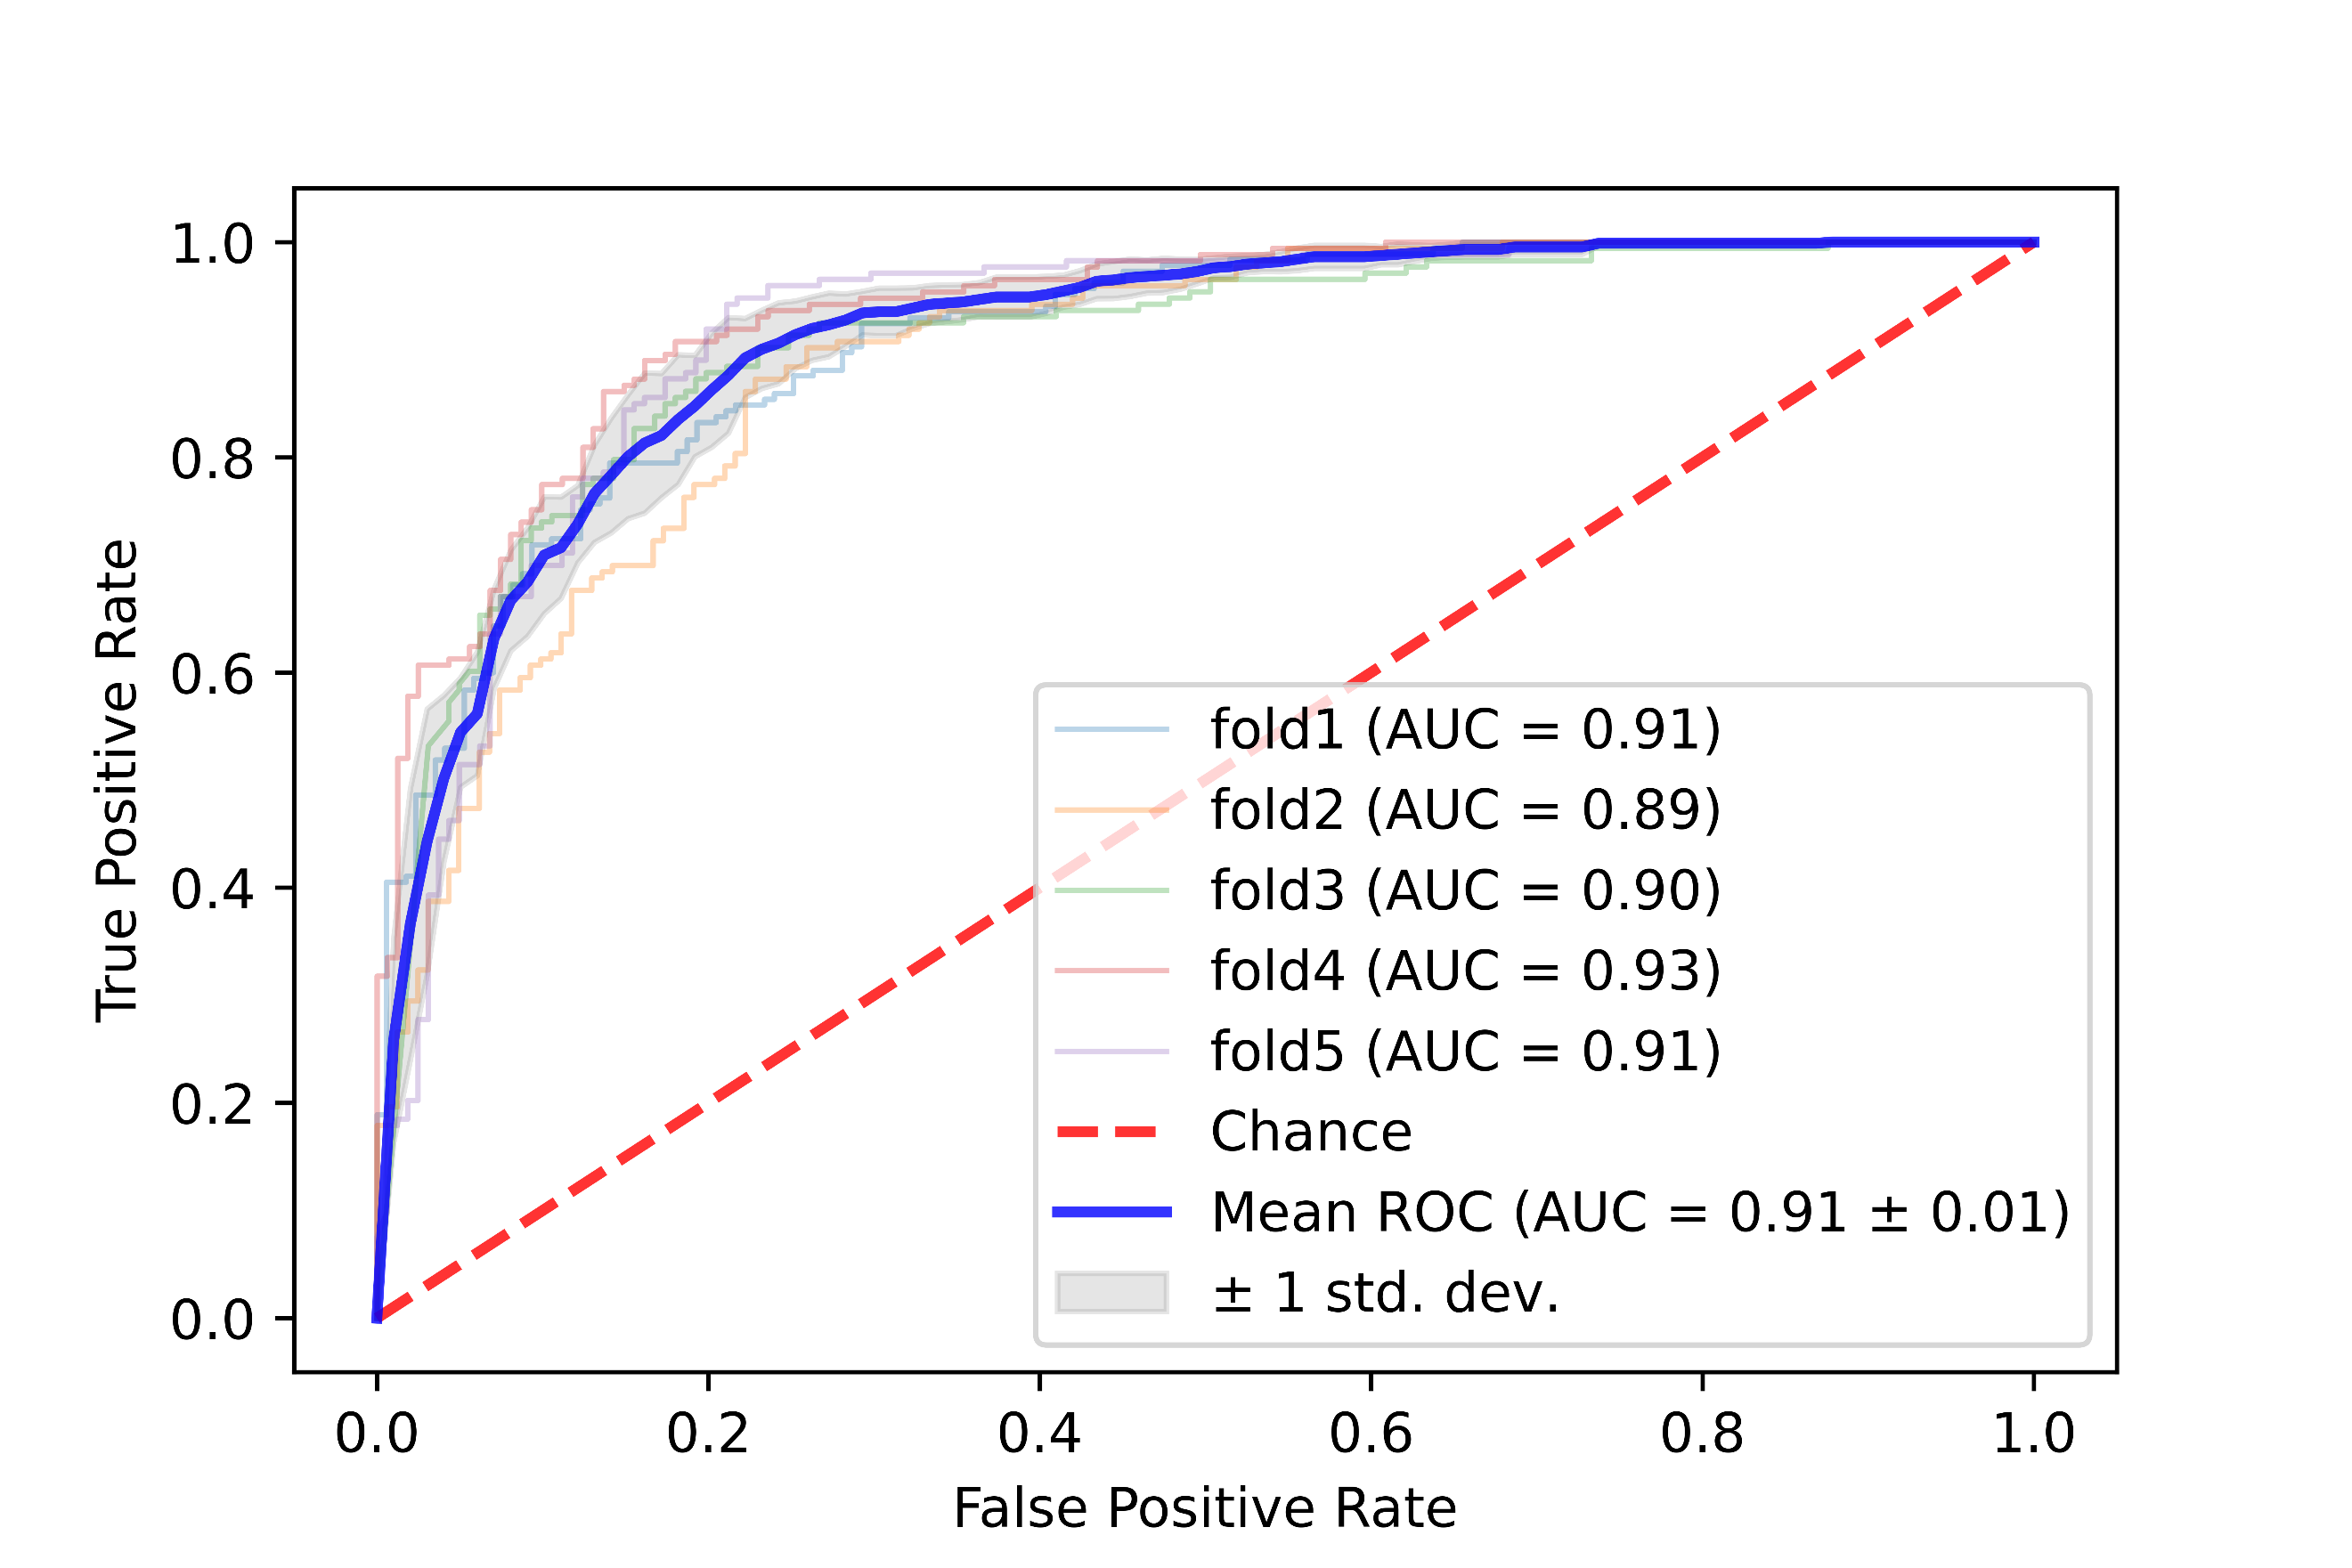
\includegraphics[width=\textwidth,keepaspectratio]{images/Supplement4/image116.png}
		\caption{ROC curve.}
	\end{subfigure}
	\hfill
	\begin{subfigure}[b]{0.49\textwidth}
		\centering
		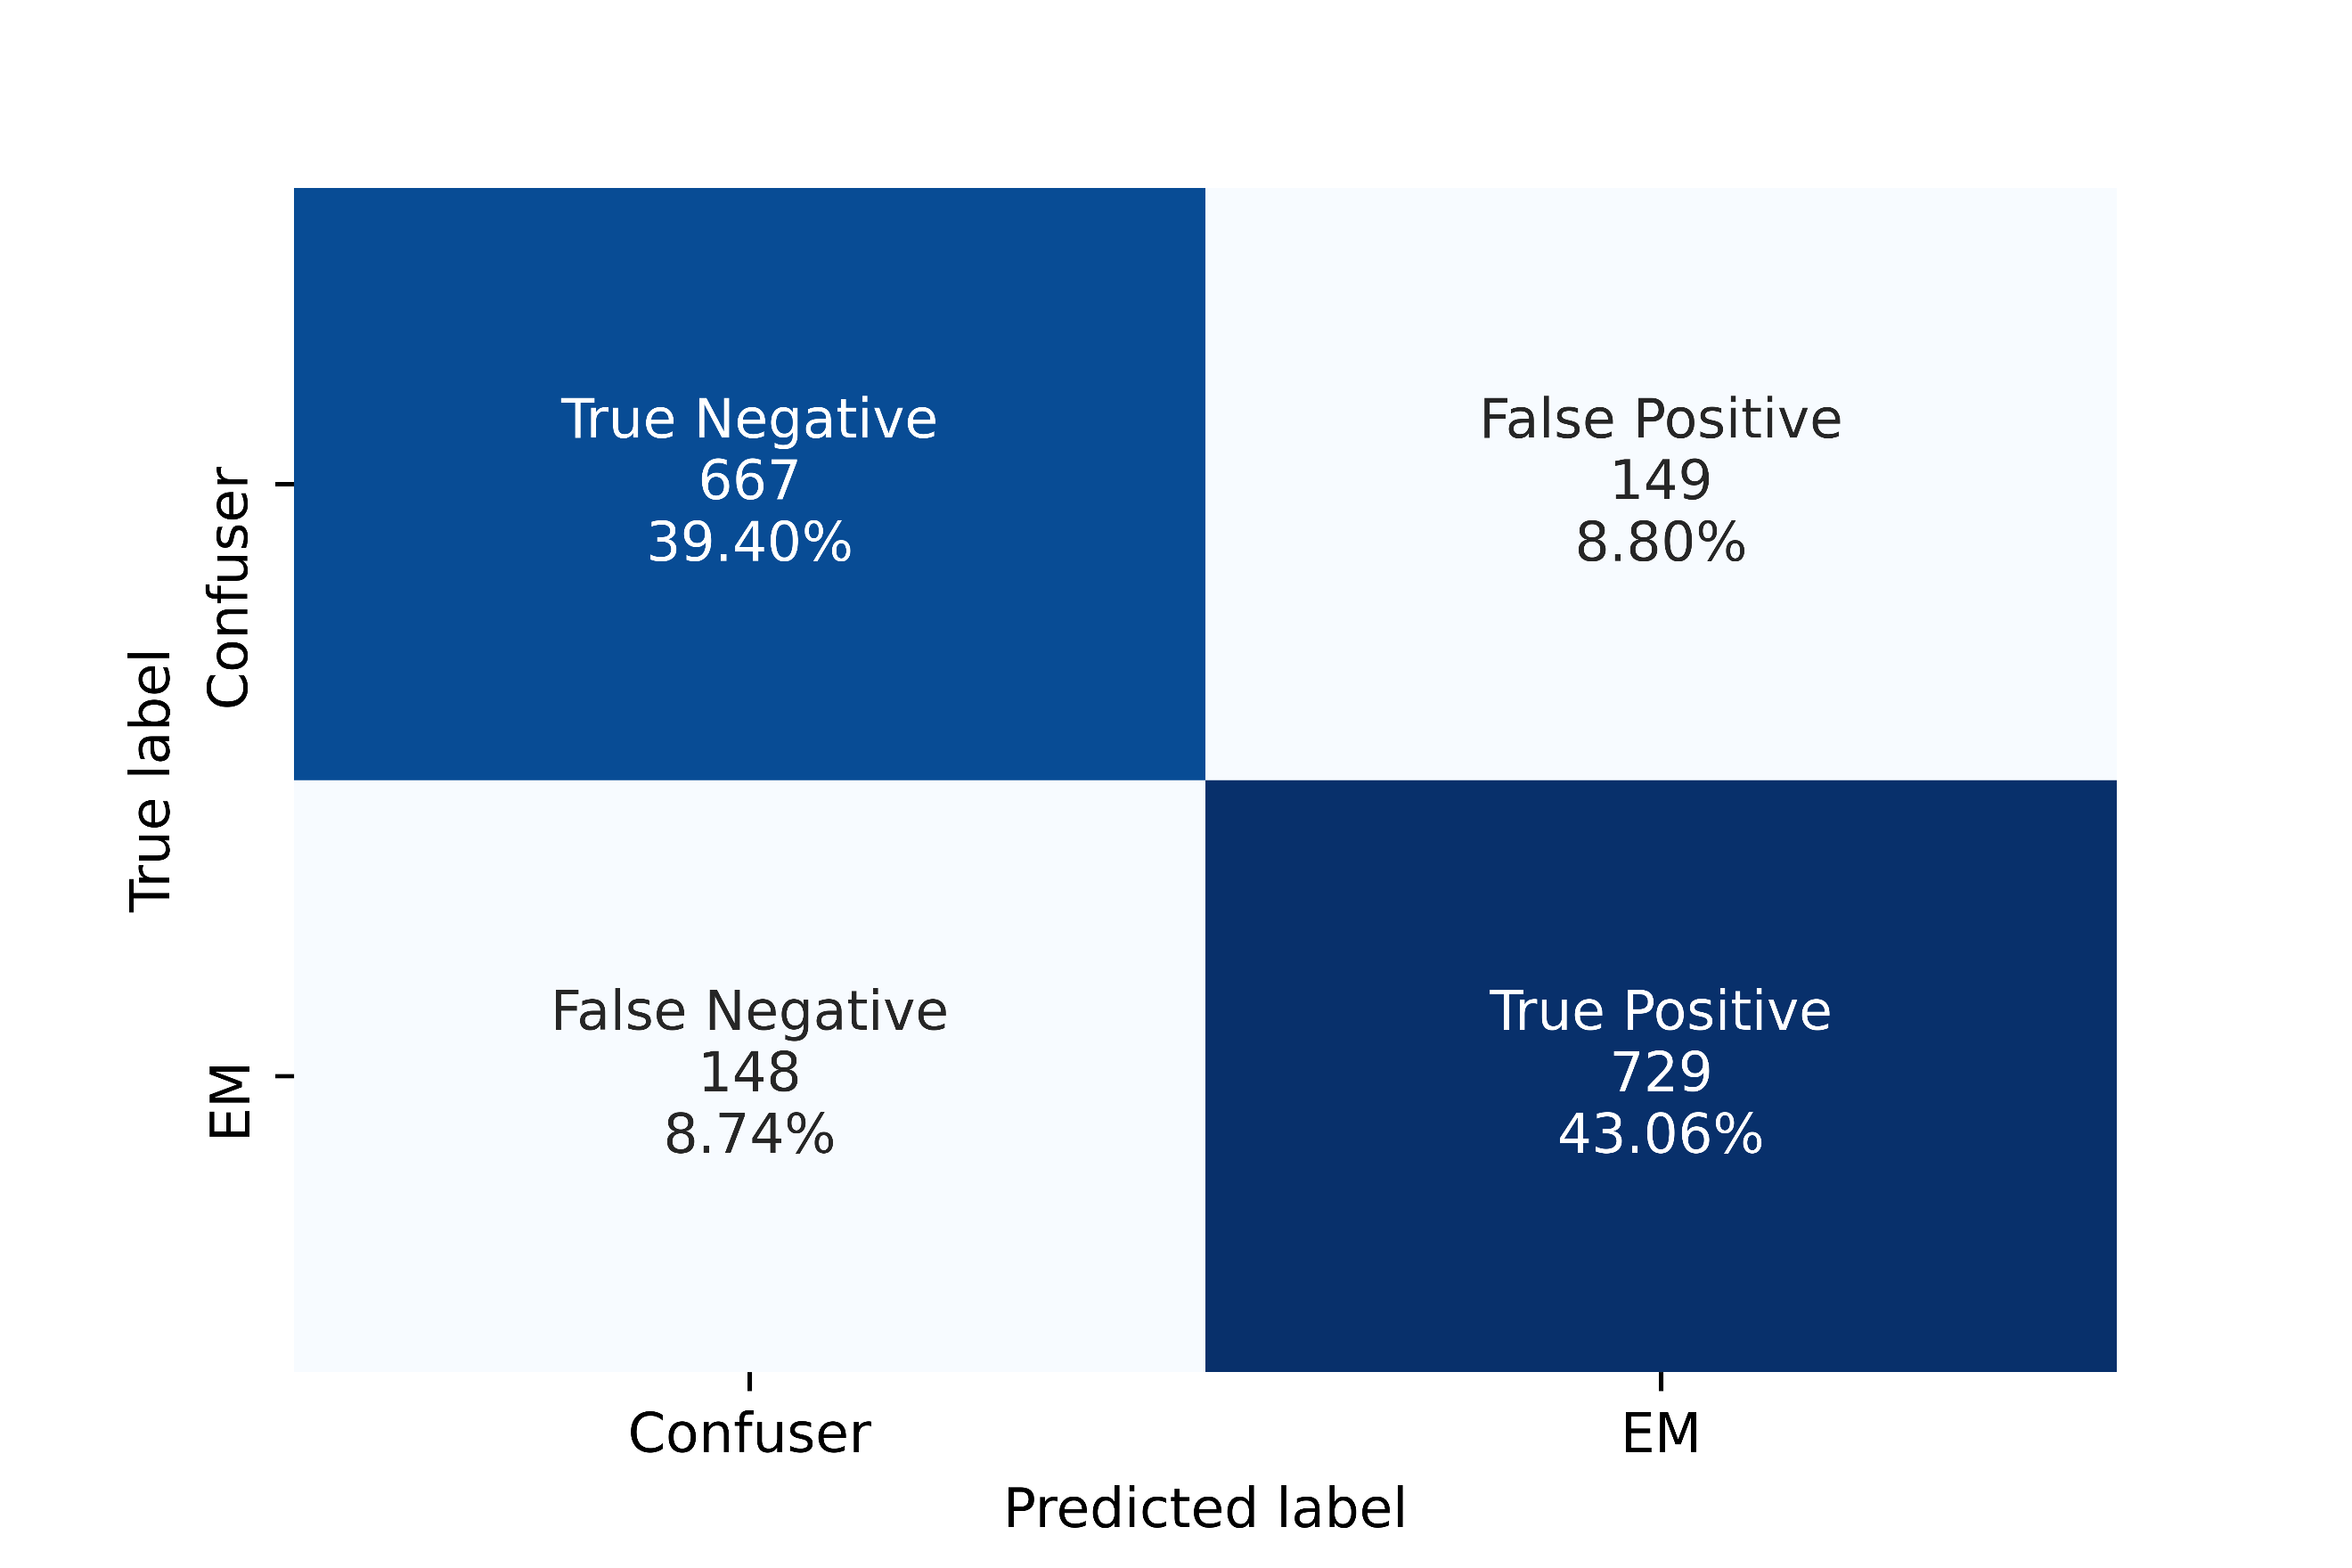
\includegraphics[width=\textwidth,keepaspectratio]{images/Supplement4/image122.png}
		\caption{Confusion matrix.}
	\end{subfigure}
	\caption{Five-fold cross-validation ROC curve and confusion matrix of Xception-118 model.}
\end{figure}

%%%%%%%%%%%%%%Break%%%%%%%%%%%%%%%%%%%%%%
\vfill\clearpage
\subsection{DenseNet121-379}

\begin{table}[h!]
	\centering
	\caption{Five-fold cross-validation performance metrics of DenseNet121-379 model.}
	\resizebox{\textwidth}{!}{%
		\begin{tabular}{llllllllllll}
			\toprule
			& \multicolumn{11}{c}{\textbf{Metric}}    \\ \cmidrule(lr){2-12} 
			\multicolumn{1}{l}{\textbf{Fold}} & \rotatebox{45}{Accuracy} & 
			\rotatebox{45}{Sensitivity} & \rotatebox{45}{Specificity} & 
			\rotatebox{45}{Precision} & \rotatebox{45}{NPV} & \rotatebox{45}{MCC} & 
			\rotatebox{45}{Kappa} & \rotatebox{45}{LR$+$} & \rotatebox{45}{LR$-$} & 
			\rotatebox{45}{F1-Score} & \rotatebox{45}{AUC}  \\ \midrule
			fold1          & 83.71 & 86.49 & 80.7  & 82.9  & 84.66 & 0.6738 & 0.6731 & 4.4816 & 0.1675 & 0.8466 & 0.9035 \\
			fold2          & 82.69 & 83.24 & 82.1  & 83.24 & 82.1  & 0.6534 & 0.6534 & 4.6498 & 0.2042 & 0.8324 & 0.9159 \\
			fold3          & 84.43 & 87.86 & 80.75 & 83.06 & 86.09 & 0.6888 & 0.6875 & 4.5631 & 0.1503 & 0.8539 & 0.9094 \\
			fold4          & 83.23 & 84.39 & 81.99 & 83.43 & 83.02 & 0.6641 & 0.6641 & 4.6853 & 0.1904 & 0.8391 & 0.9178 \\
			fold5          & 85.33 & 87.28 & 83.23 & 84.83 & 85.9  & 0.7062 & 0.7059 & 5.2047 & 0.1528 & 0.8604 & 0.9325 \\\cmidrule(lr){1-12}
			average        & 83.88 & 85.85 & 81.75 & 83.49 & 84.35 & 0.6773 & 0.6768 & 4.7169 & 0.173  & 0.8465 & 0.9158 \\
			std. deviation & 0.92  & 1.76  & 0.95  & 0.69  & 1.57  & 0.0186 & 0.0184 & 0.254  & 0.0211 & 0.01   & 0.0097\\
			\bottomrule
		\end{tabular}%
	}
\end{table}


\begin{figure}[h!]
	\centering
	\begin{subfigure}[b]{0.49\textwidth}
		\centering
		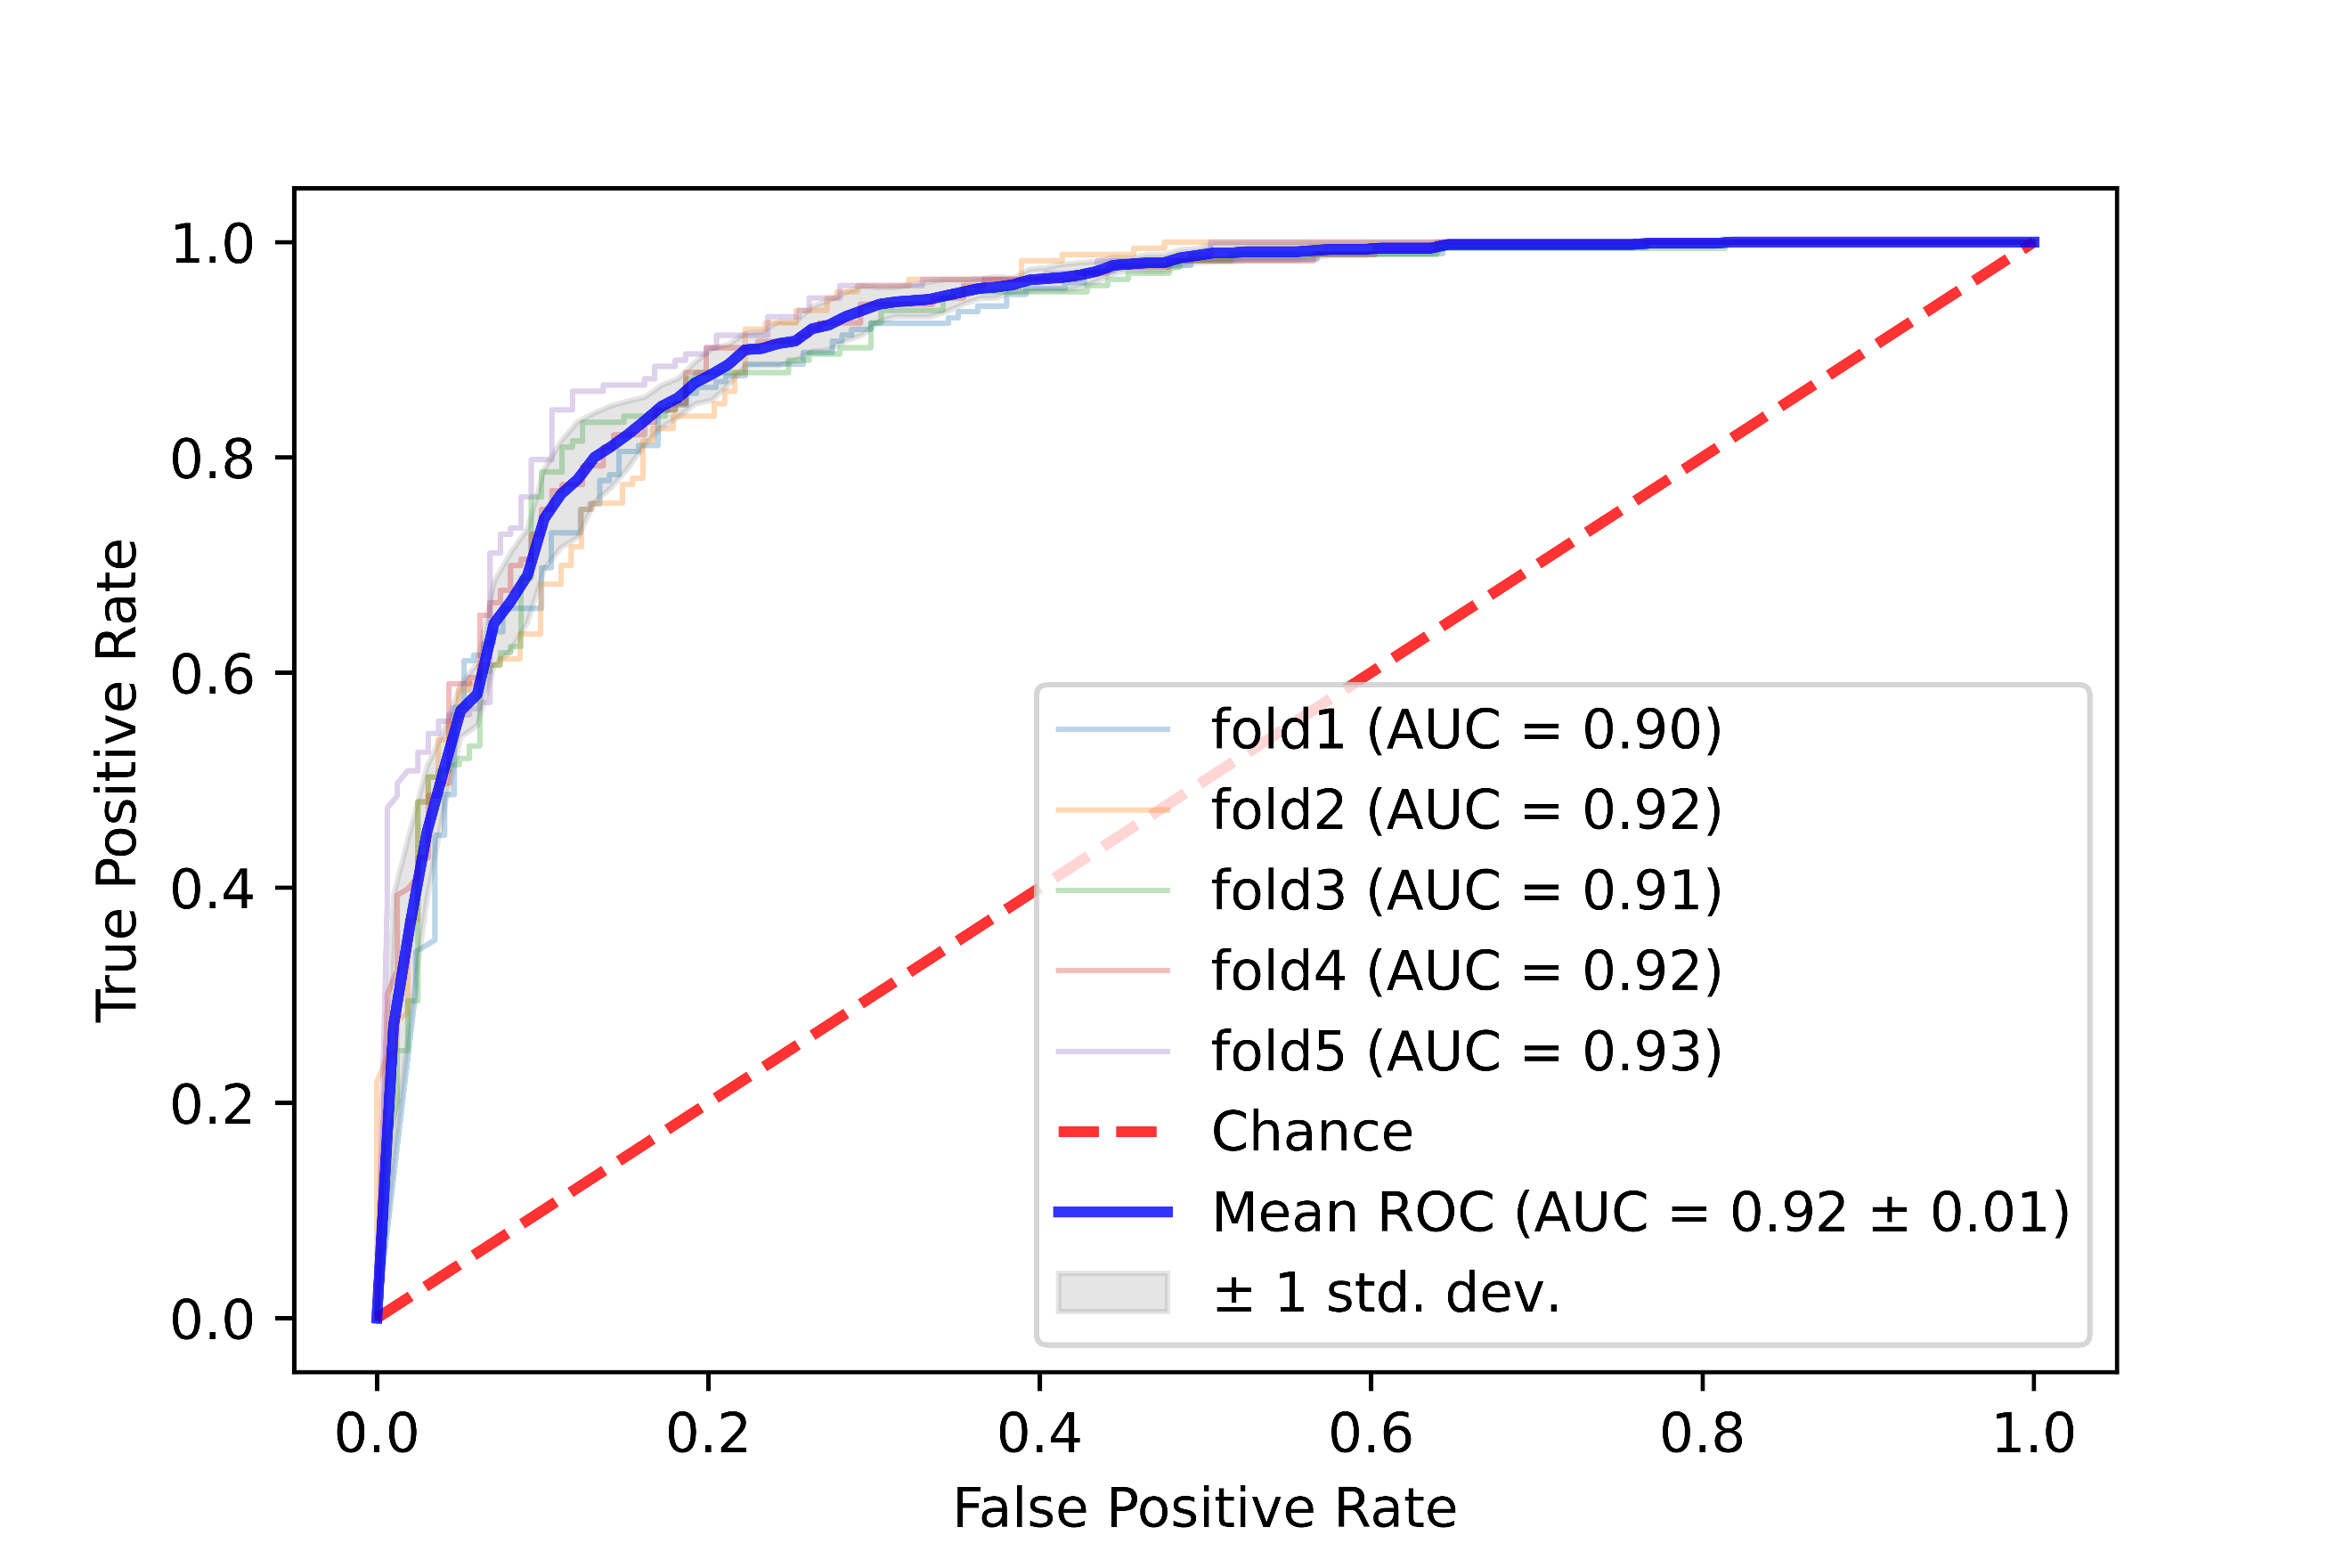
\includegraphics[width=\textwidth,keepaspectratio]{images/Supplement4/image123.png}
		\caption{ROC curve.}
	\end{subfigure}
	\hfill
	\begin{subfigure}[b]{0.49\textwidth}
		\centering
		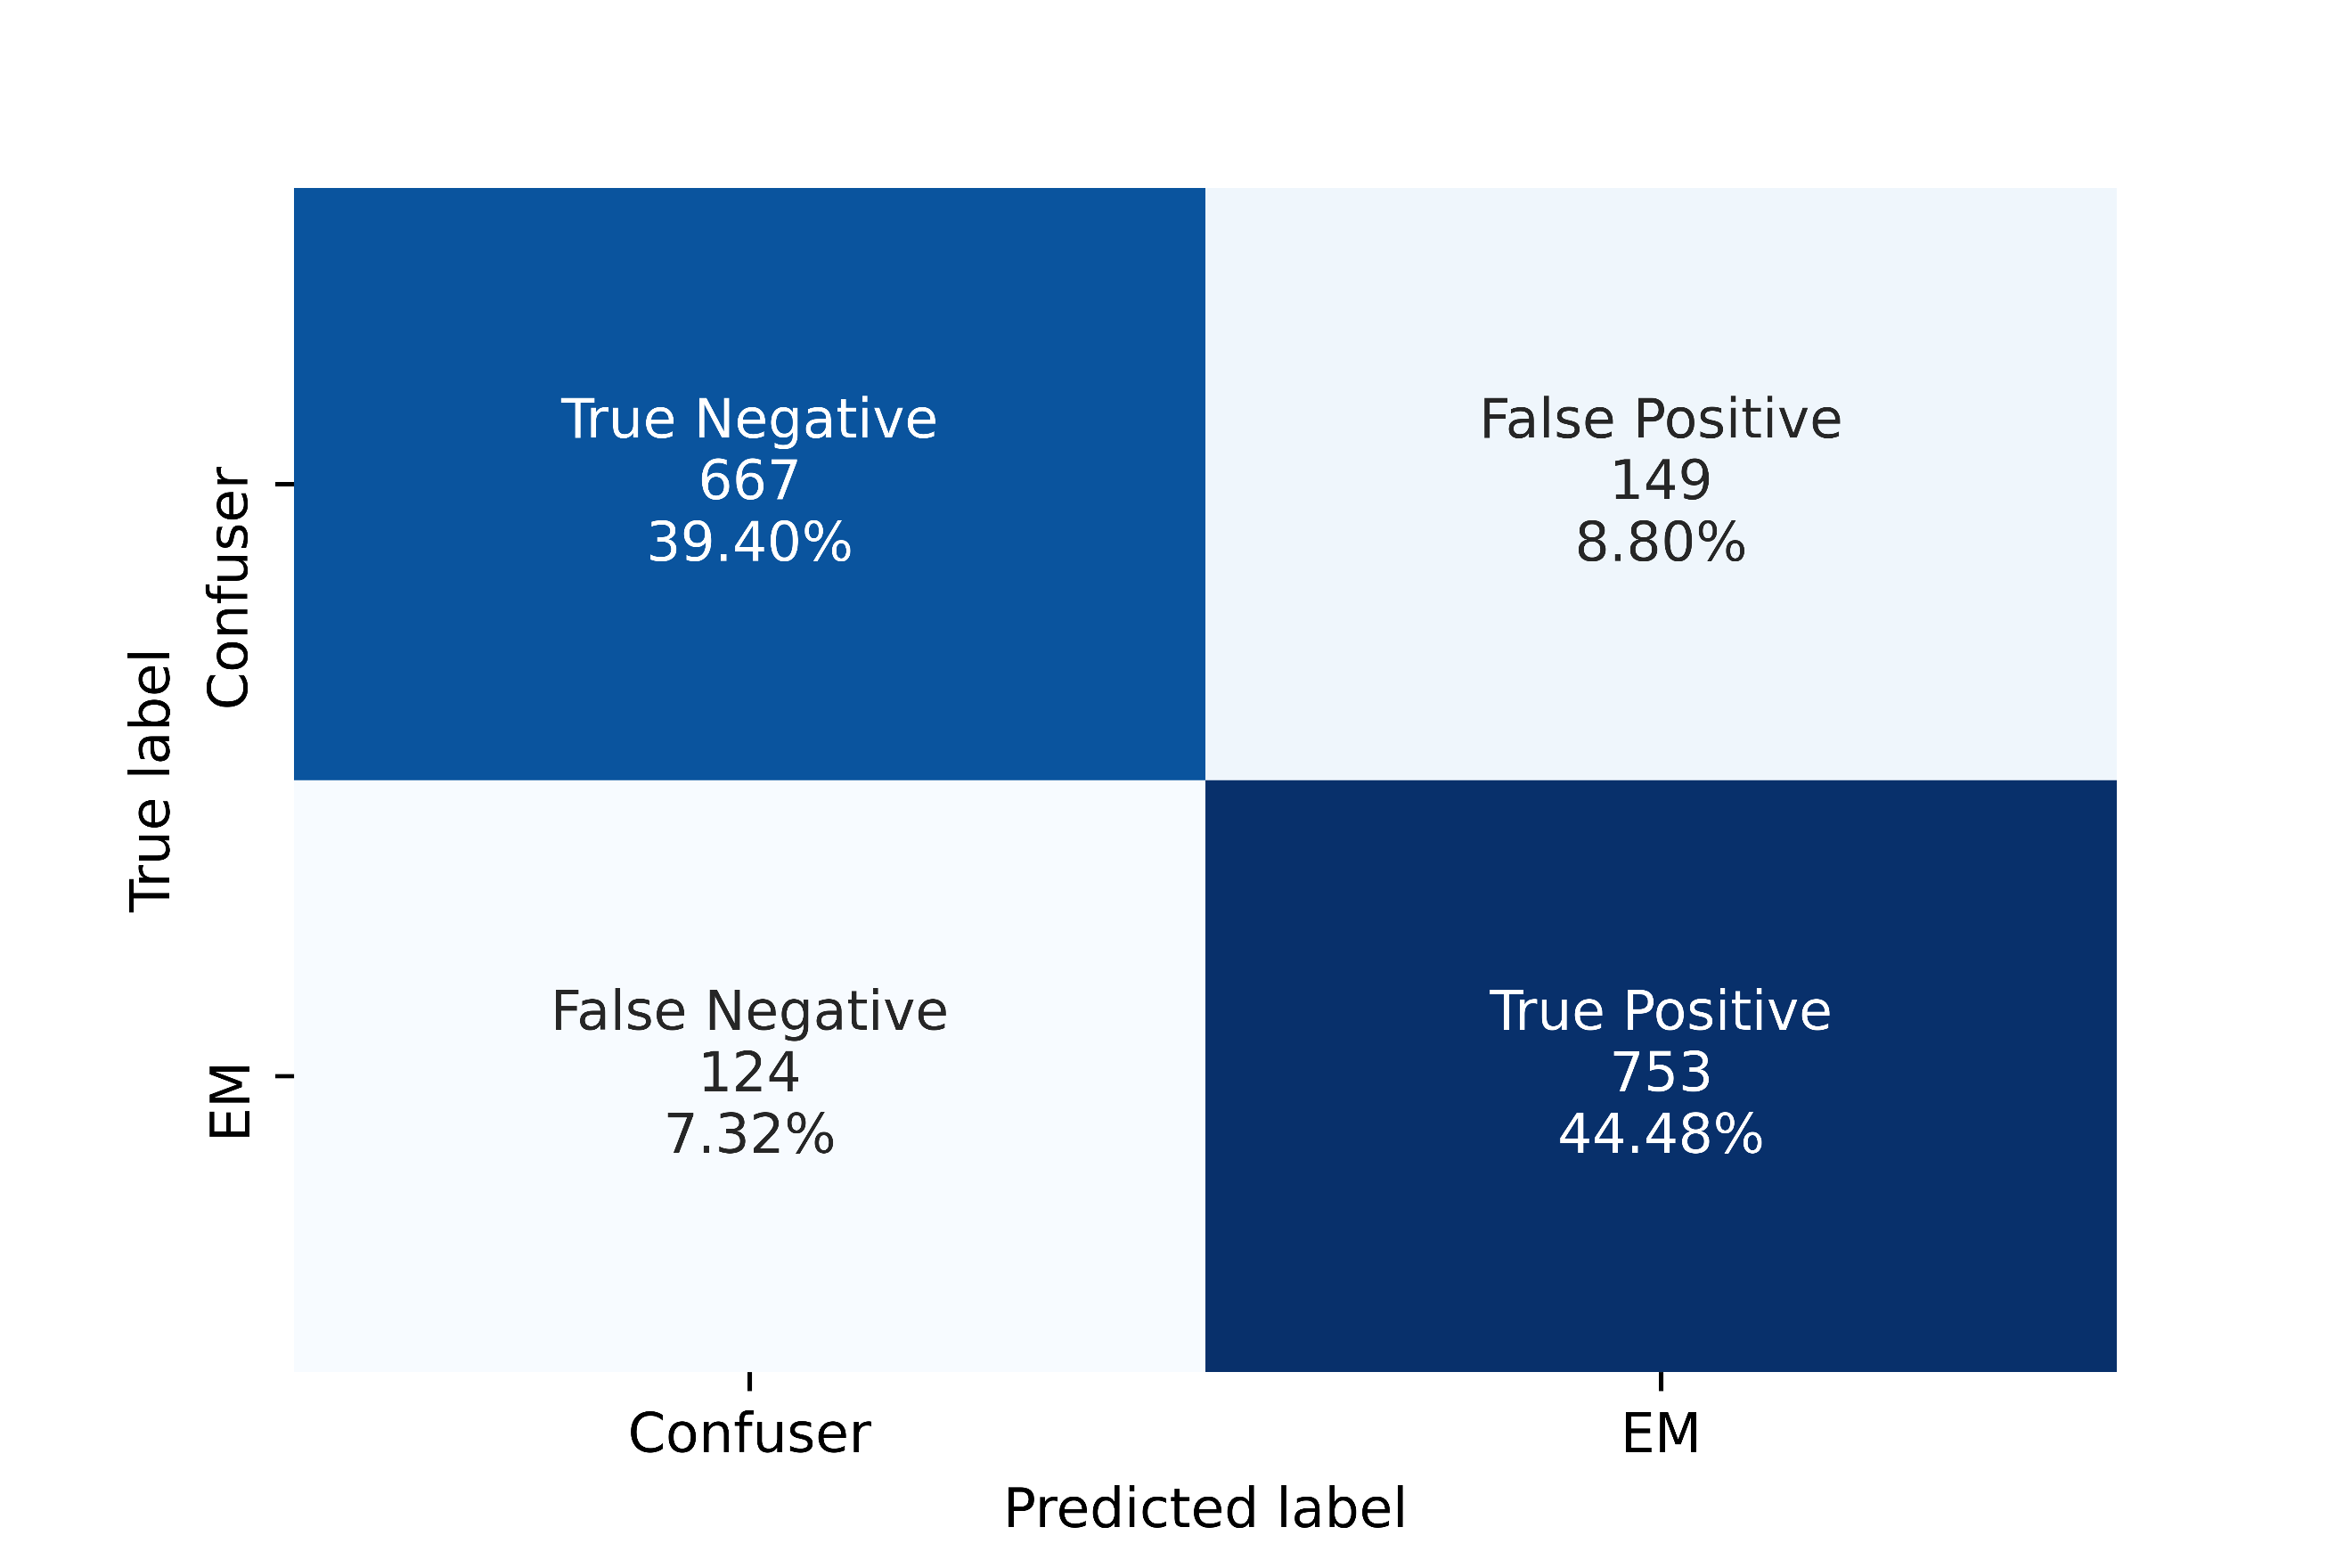
\includegraphics[width=\textwidth,keepaspectratio]{images/Supplement4/image129.png}
		\caption{Confusion matrix.}
	\end{subfigure}
	\caption{Five-fold cross-validation ROC curve and confusion matrix of DenseNet121-379 model.}
\end{figure}

%%%%%%%%%%%%%%Break%%%%%%%%%%%%%%%%%%%%%%
\vfill\clearpage
\subsection{DenseNet169-395}

\begin{table}[h!]
	\centering
	\caption{Five-fold cross-validation performance metrics of DenseNet169-395 model.}
	\resizebox{\textwidth}{!}{%
		\begin{tabular}{llllllllllll}
			\toprule
			& \multicolumn{11}{c}{\textbf{Metric}}    \\ \cmidrule(lr){2-12} 
			\multicolumn{1}{l}{\textbf{Fold}} & \rotatebox{45}{Accuracy} & 
			\rotatebox{45}{Sensitivity} & \rotatebox{45}{Specificity} & 
			\rotatebox{45}{Precision} & \rotatebox{45}{NPV} & \rotatebox{45}{MCC} & 
			\rotatebox{45}{Kappa} & \rotatebox{45}{LR$+$} & \rotatebox{45}{LR$-$} & 
			\rotatebox{45}{F1-Score} & \rotatebox{45}{AUC}  \\ \midrule
			fold1          & 82.02 & 88.65 & 74.85 & 79.23 & 85.91 & 0.6431 & 0.6381 & 3.5253 & 0.1516 & 0.8367 & 0.8996 \\
			fold2          & 84.78 & 93.06 & 75.93 & 80.5  & 91.11 & 0.7029 & 0.6936 & 3.8657 & 0.0914 & 0.8633 & 0.9124 \\
			fold3          & 83.53 & 87.28 & 79.5  & 82.07 & 85.33 & 0.6709 & 0.6694 & 4.2584 & 0.16   & 0.8459 & 0.8964 \\
			fold4          & 85.33 & 91.33 & 78.88 & 82.29 & 89.44 & 0.7097 & 0.705  & 4.3247 & 0.1099 & 0.8658 & 0.9269 \\
			fold5          & 82.63 & 82.66 & 82.61 & 83.63 & 81.6  & 0.6524 & 0.6524 & 4.7529 & 0.2099 & 0.8314 & 0.9264 \\\cmidrule(lr){1-12}
			average        & 83.66 & 88.6  & 78.35 & 81.54 & 86.68 & 0.6758 & 0.6717 & 4.1454 & 0.1446 & 0.8486 & 0.9123 \\
			std. deviation & 1.25  & 3.59  & 2.75  & 1.53  & 3.33  & 0.0265 & 0.0249 & 0.4187 & 0.0414 & 0.0138 & 0.0129\\
			\bottomrule
		\end{tabular}%
	}
\end{table}


\begin{figure}[h!]
	\centering
	\begin{subfigure}[b]{0.49\textwidth}
		\centering
		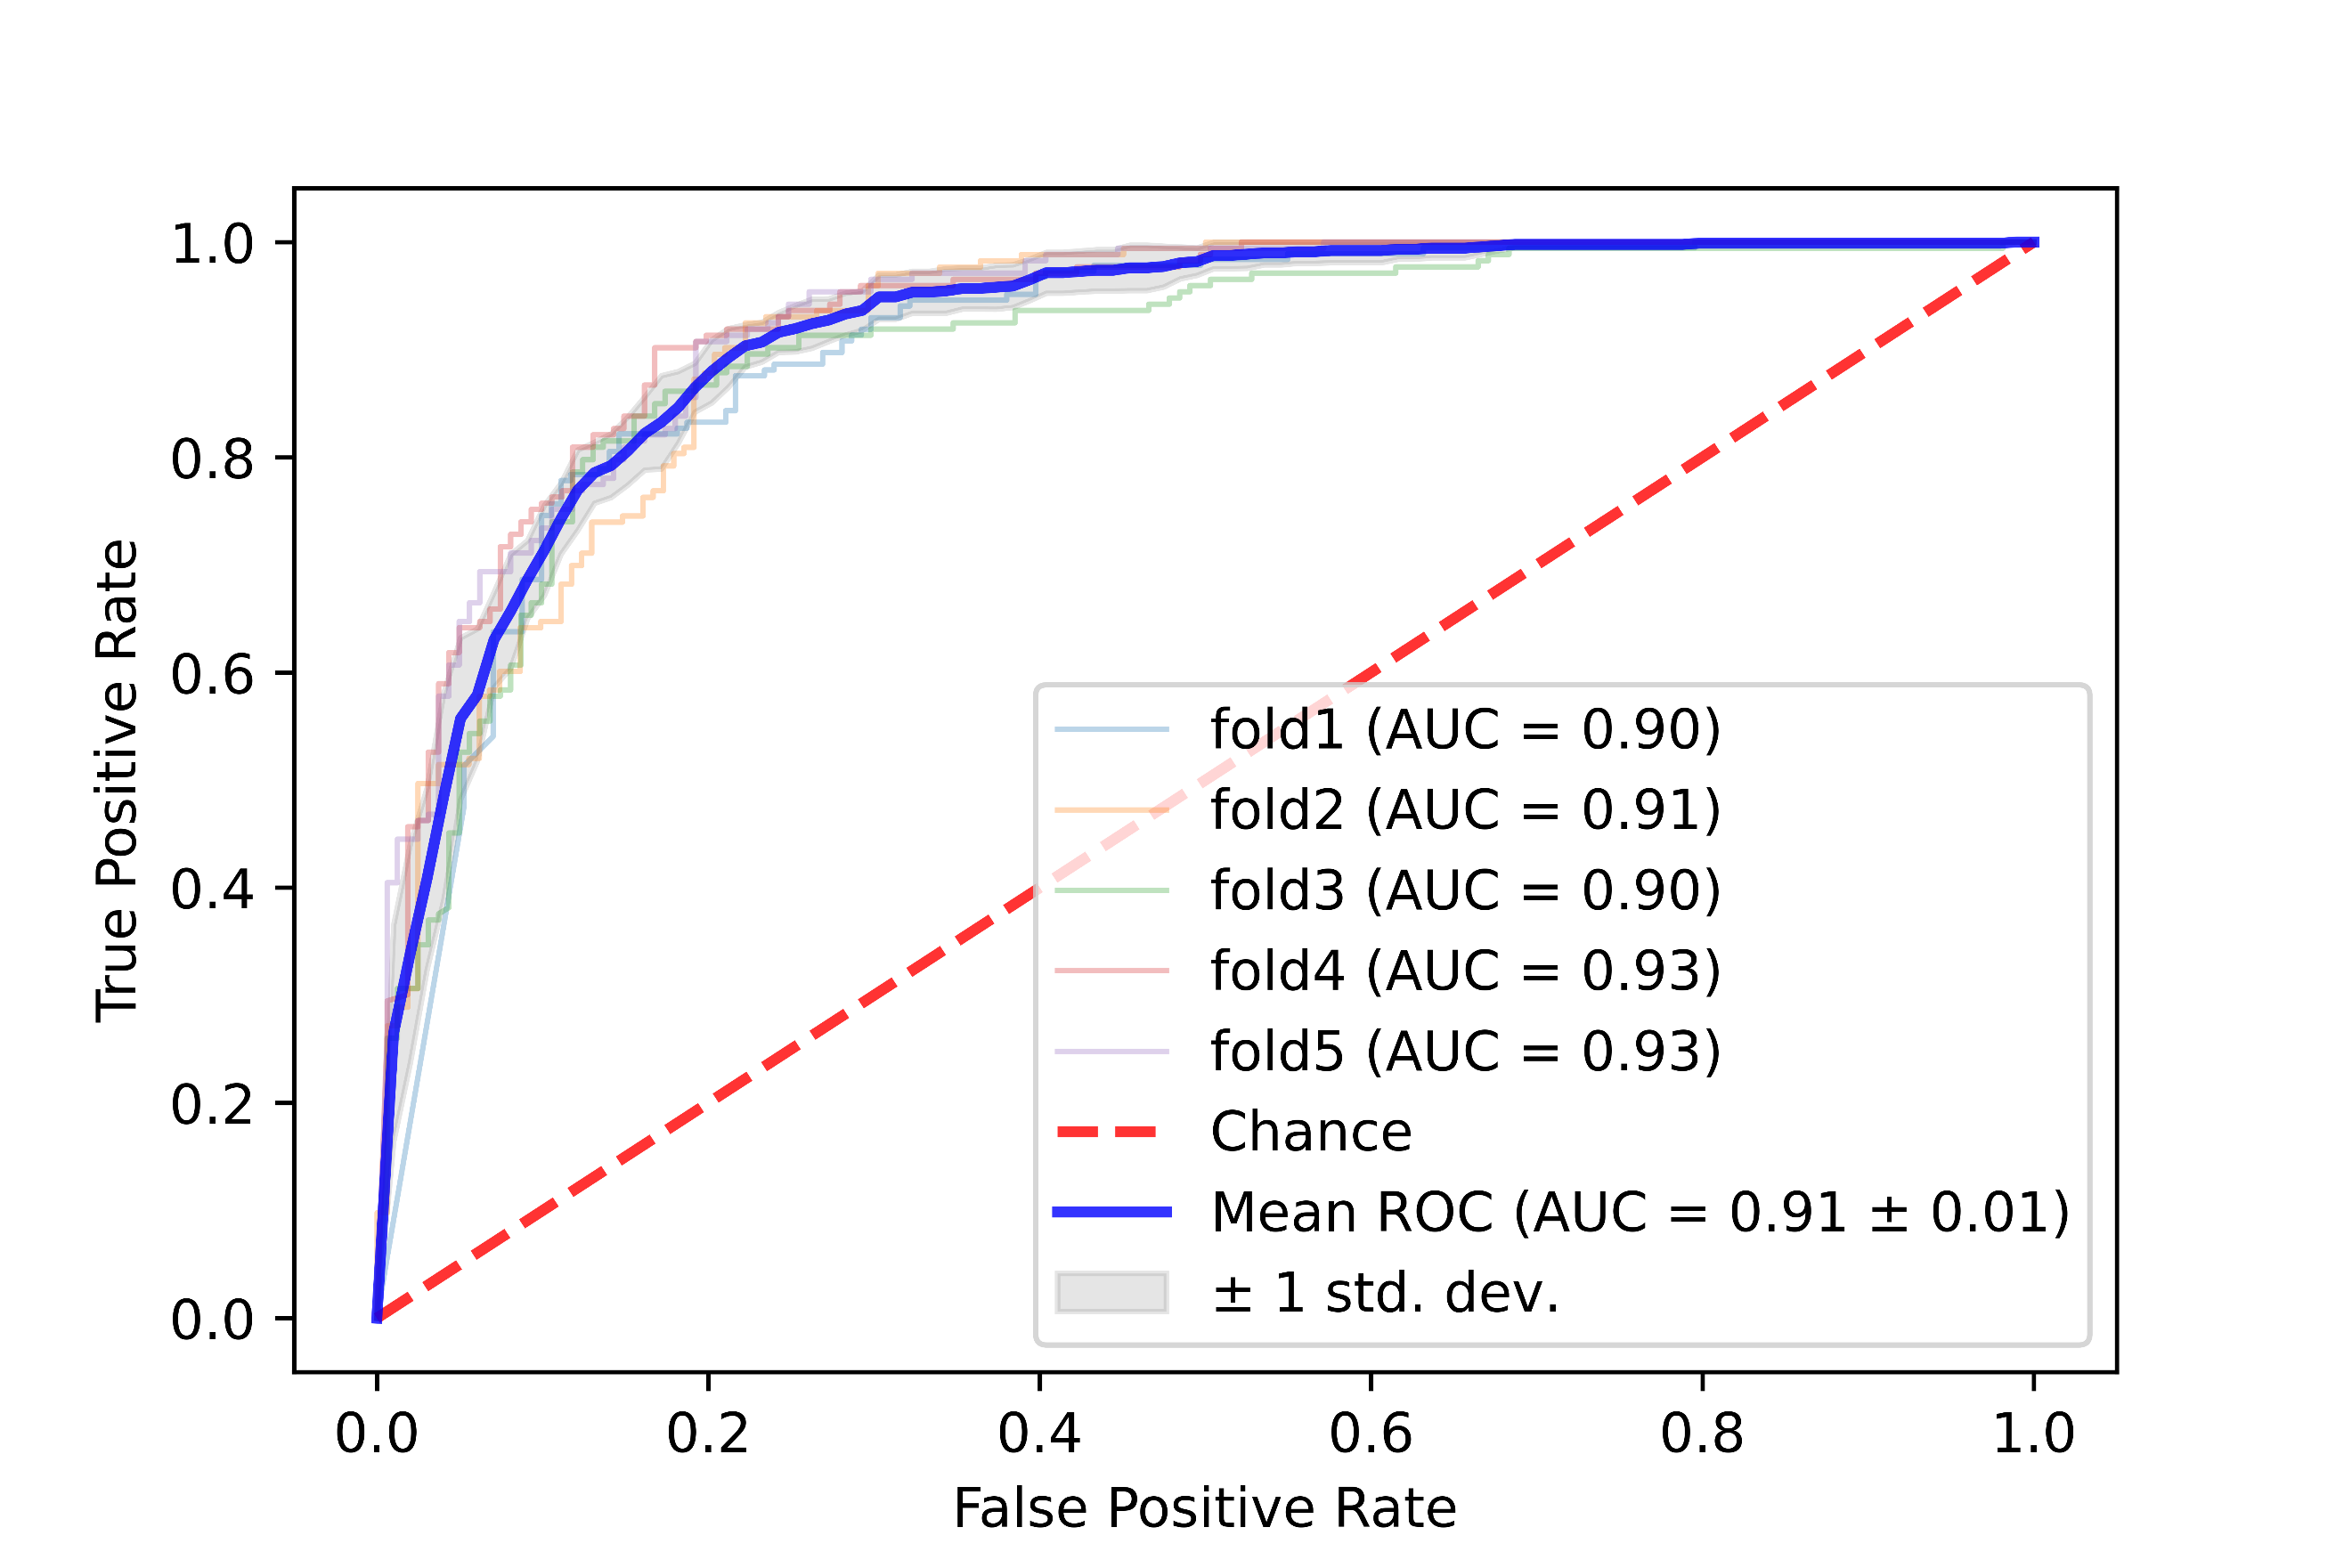
\includegraphics[width=\textwidth,keepaspectratio]{images/Supplement4/image130.png}
		\caption{ROC curve.}
	\end{subfigure}
	\hfill
	\begin{subfigure}[b]{0.49\textwidth}
		\centering
		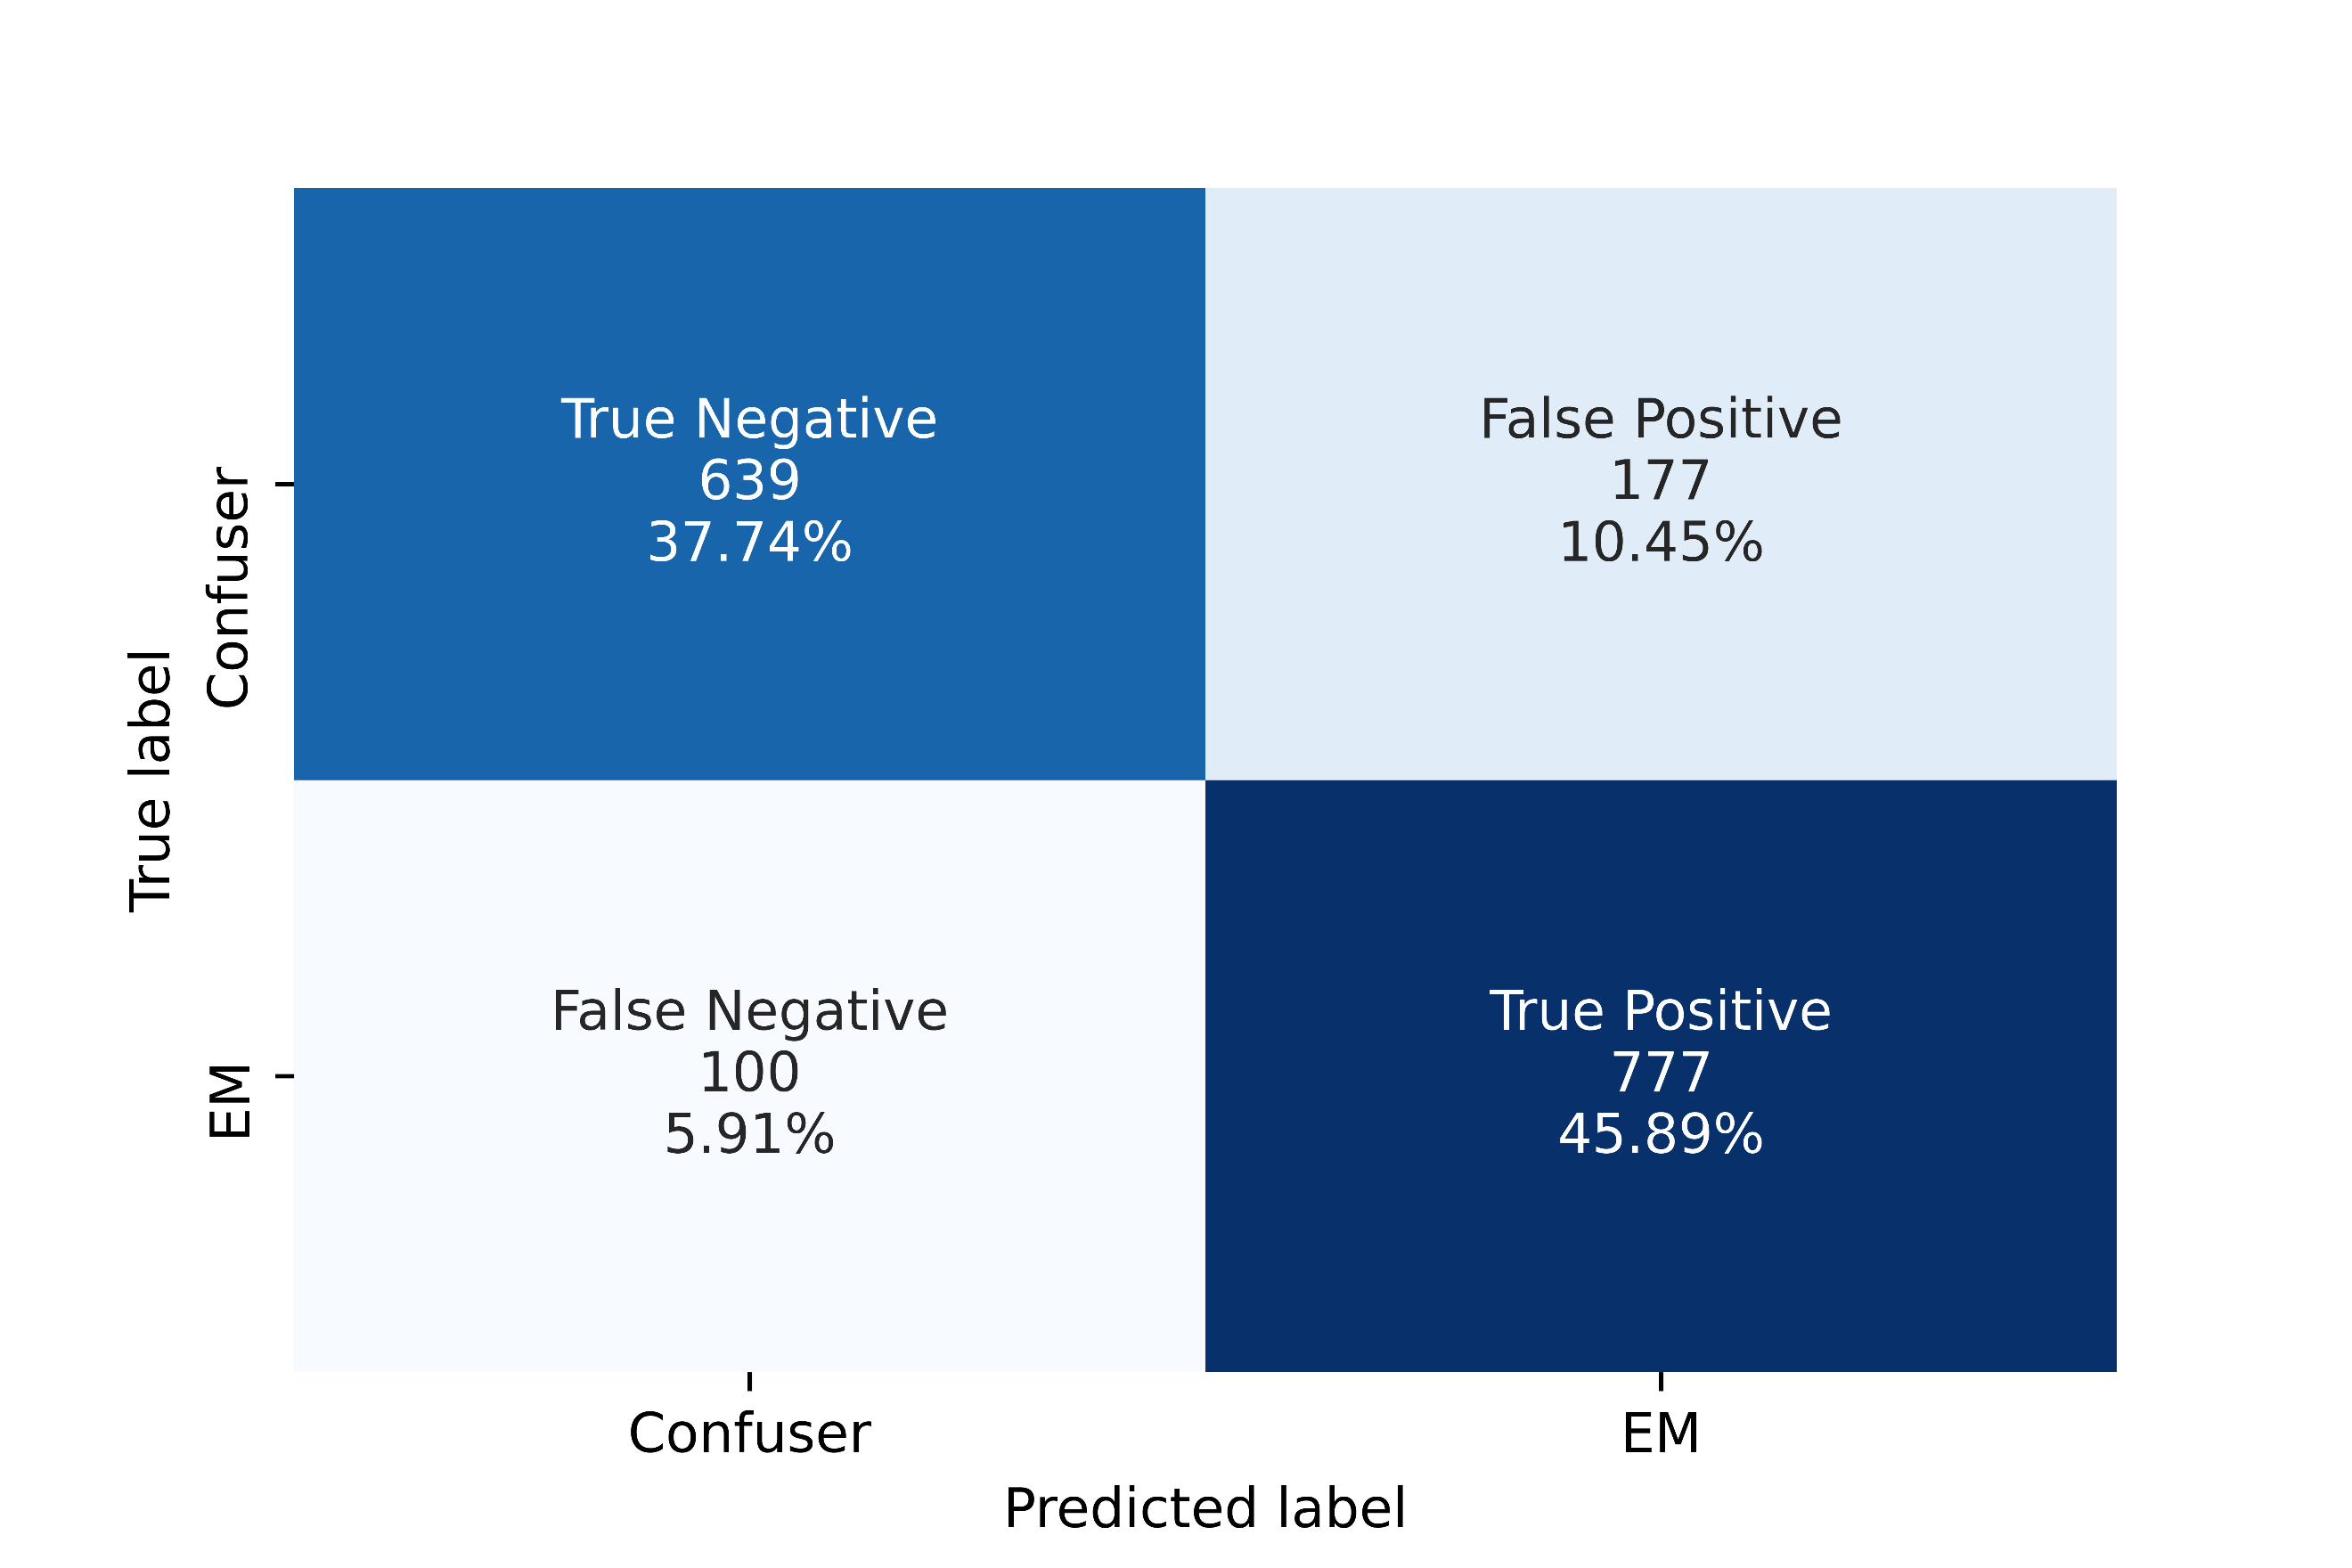
\includegraphics[width=\textwidth,keepaspectratio]{images/Supplement4/image135.png}
		\caption{Confusion matrix.}
	\end{subfigure}
	\caption{Five-fold cross-validation ROC curve and confusion matrix of DenseNet169-395 model.}
\end{figure}

%%%%%%%%%%%%%%Break%%%%%%%%%%%%%%%%%%%%%%
\vfill\clearpage
\subsection{DenseNet201-561}

\begin{table}[h!]
	\centering
	\caption{Five-fold cross-validation performance metrics of DenseNet201-561 model.}
	\resizebox{\textwidth}{!}{%
		\begin{tabular}{llllllllllll}
			\toprule
			& \multicolumn{11}{c}{\textbf{Metric}}    \\ \cmidrule(lr){2-12} 
			\multicolumn{1}{l}{\textbf{Fold}} & \rotatebox{45}{Accuracy} & 
			\rotatebox{45}{Sensitivity} & \rotatebox{45}{Specificity} & 
			\rotatebox{45}{Precision} & \rotatebox{45}{NPV} & \rotatebox{45}{MCC} & 
			\rotatebox{45}{Kappa} & \rotatebox{45}{LR$+$} & \rotatebox{45}{LR$-$} & 
			\rotatebox{45}{F1-Score} & \rotatebox{45}{AUC}  \\ \midrule
			fold1          & 82.02 & 87.57 & 76.02 & 79.8  & 84.97 & 0.6418 & 0.6385 & 3.6522 & 0.1635 & 0.8351 & 0.9073 \\
			fold2          & 82.09 & 84.97 & 79.01 & 81.22 & 83.12 & 0.6416 & 0.6408 & 4.0486 & 0.1902 & 0.8305 & 0.9016 \\
			fold3          & 82.93 & 87.86 & 77.64 & 80.85 & 85.62 & 0.6598 & 0.6571 & 3.9294 & 0.1563 & 0.8421 & 0.9093 \\
			fold4          & 83.53 & 84.39 & 82.61 & 83.91 & 83.12 & 0.6702 & 0.6702 & 4.8526 & 0.1889 & 0.8415 & 0.9223 \\
			fold5          & 85.03 & 83.24 & 86.96 & 87.27 & 82.84 & 0.7015 & 0.7007 & 6.3815 & 0.1928 & 0.8521 & 0.922  \\\cmidrule(lr){1-12}
			average        & 83.12 & 85.61 & 80.45 & 82.61 & 83.93 & 0.663  & 0.6615 & 4.5729 & 0.1783 & 0.8403 & 0.9125 \\
			std. deviation & 1.11  & 1.81  & 3.92  & 2.7   & 1.13  & 0.0221 & 0.0228 & 0.9885 & 0.0153 & 0.0073 & 0.0083\\
			\bottomrule
		\end{tabular}%
	}
\end{table}


\begin{figure}[h!]
	\centering
	\begin{subfigure}[b]{0.49\textwidth}
		\centering
		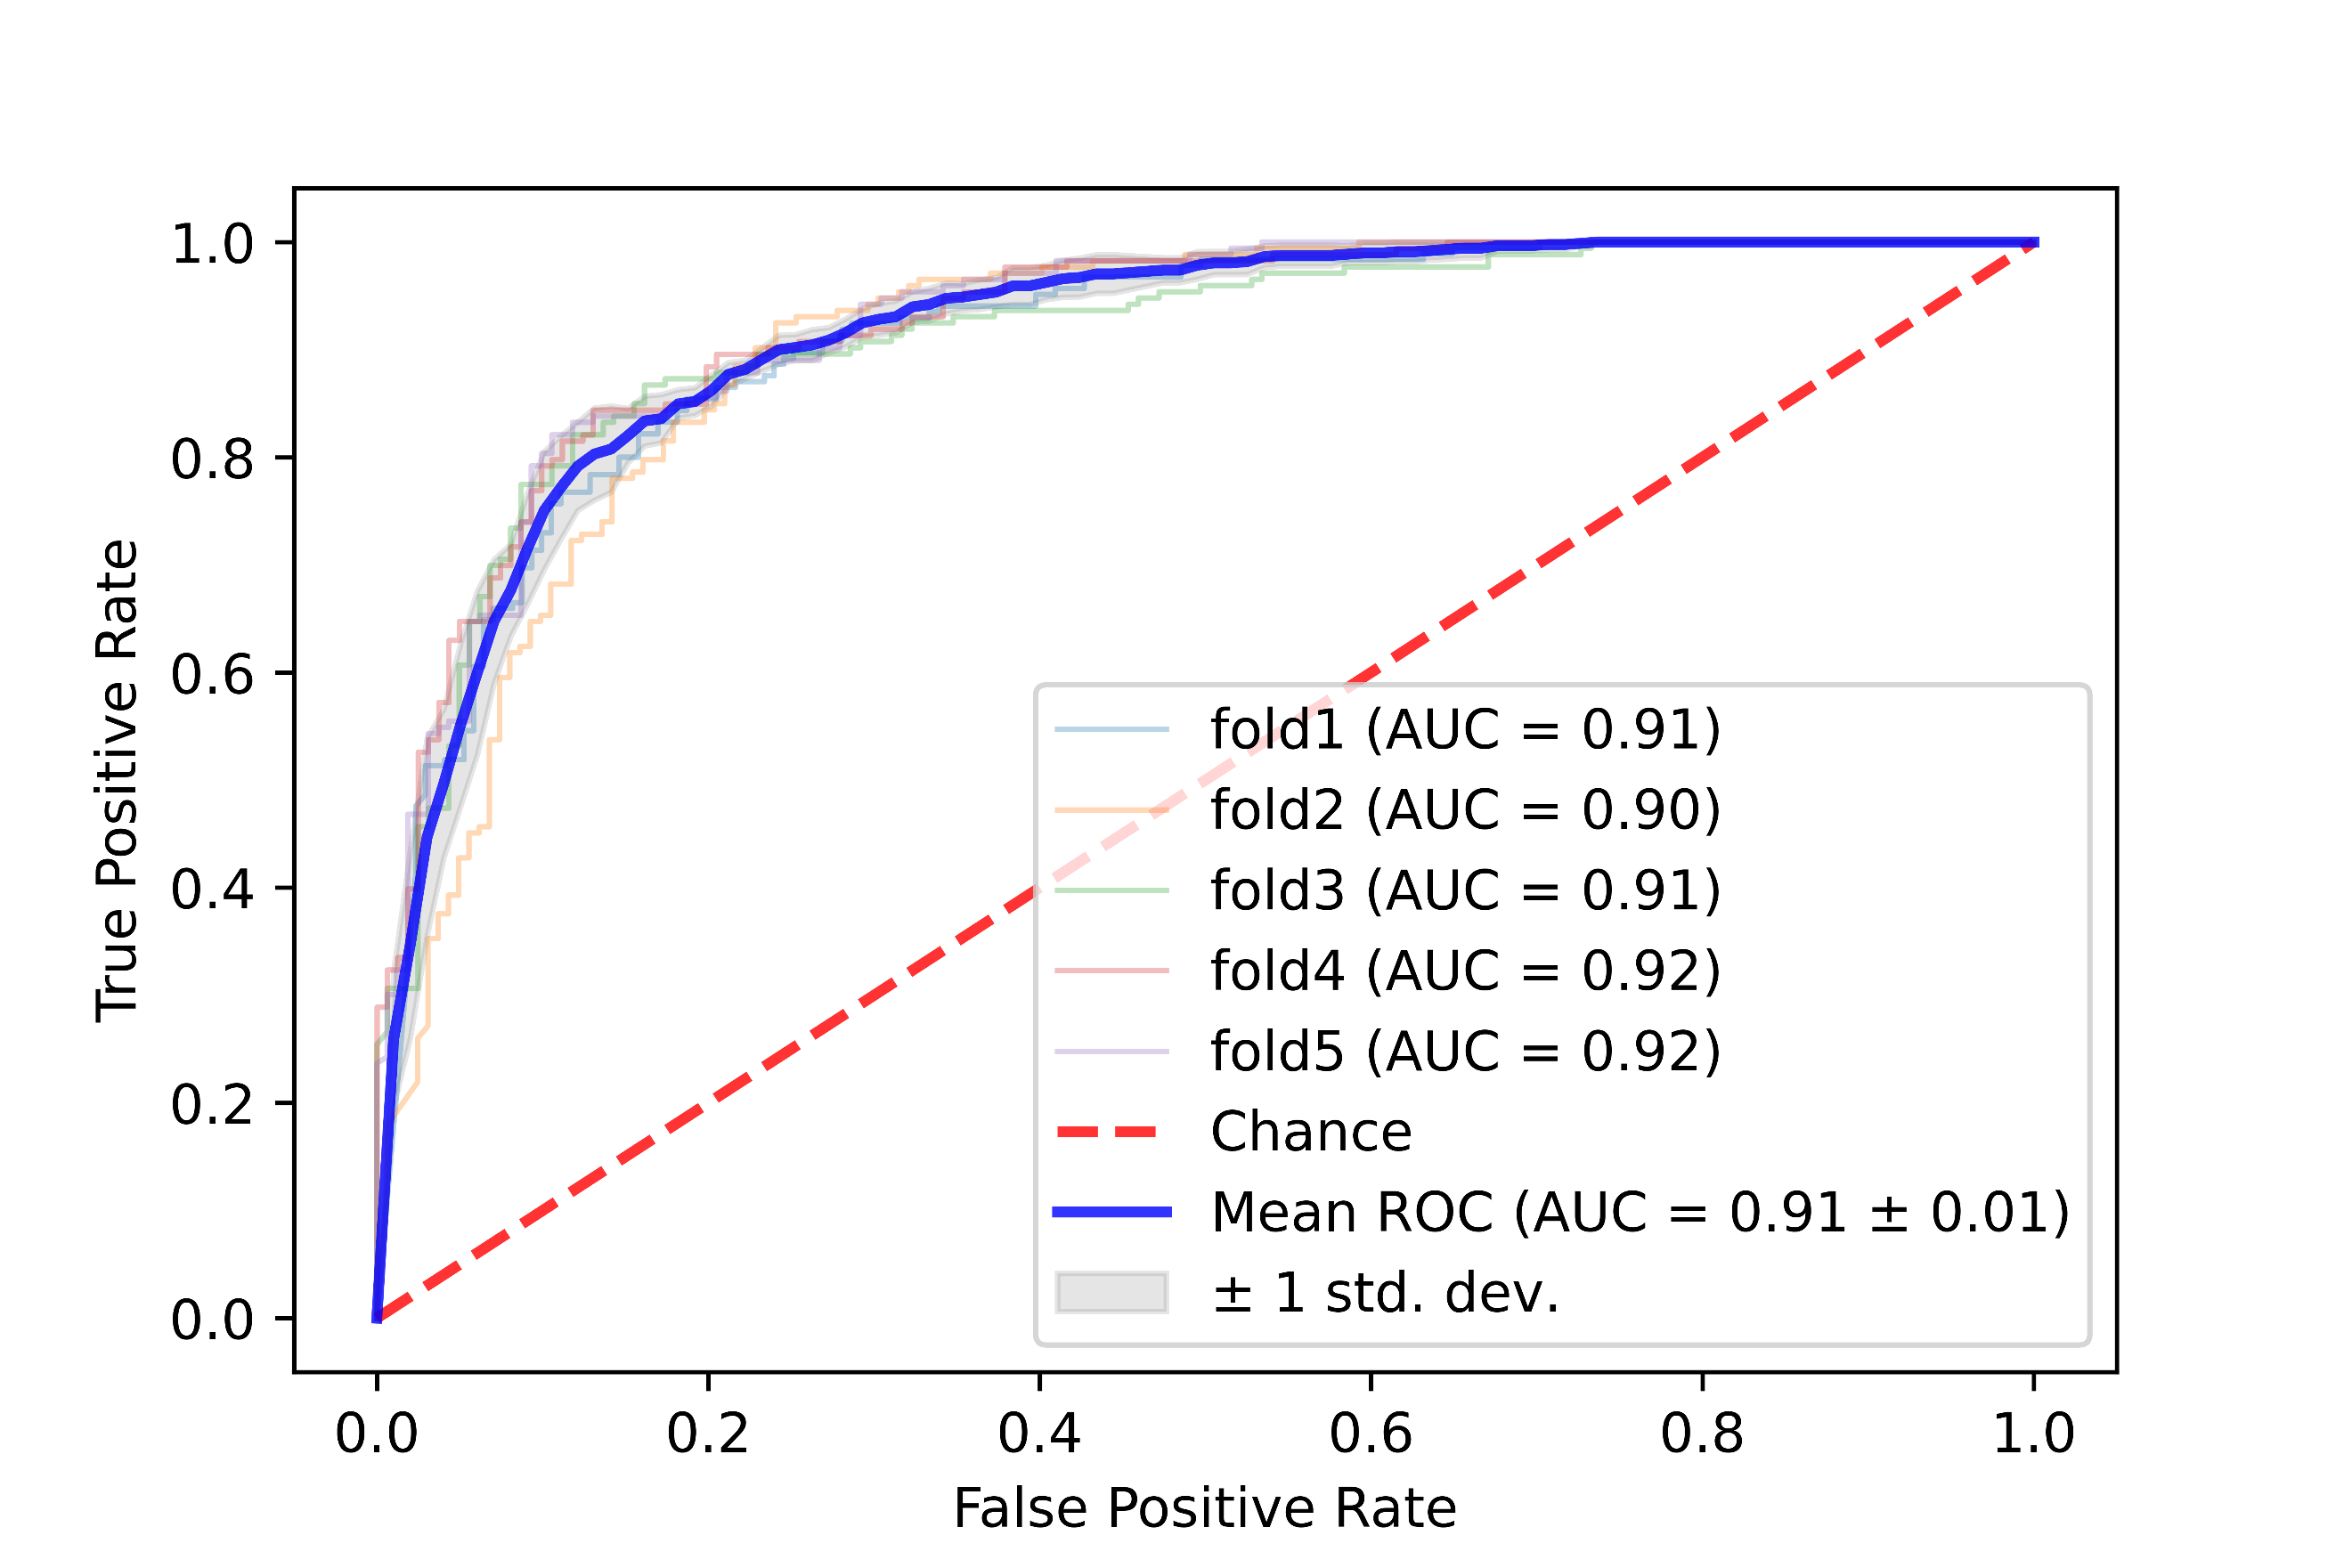
\includegraphics[width=\textwidth,keepaspectratio]{images/Supplement4/image136.png}
		\caption{ROC curve.}
	\end{subfigure}
	\hfill
	\begin{subfigure}[b]{0.49\textwidth}
		\centering
		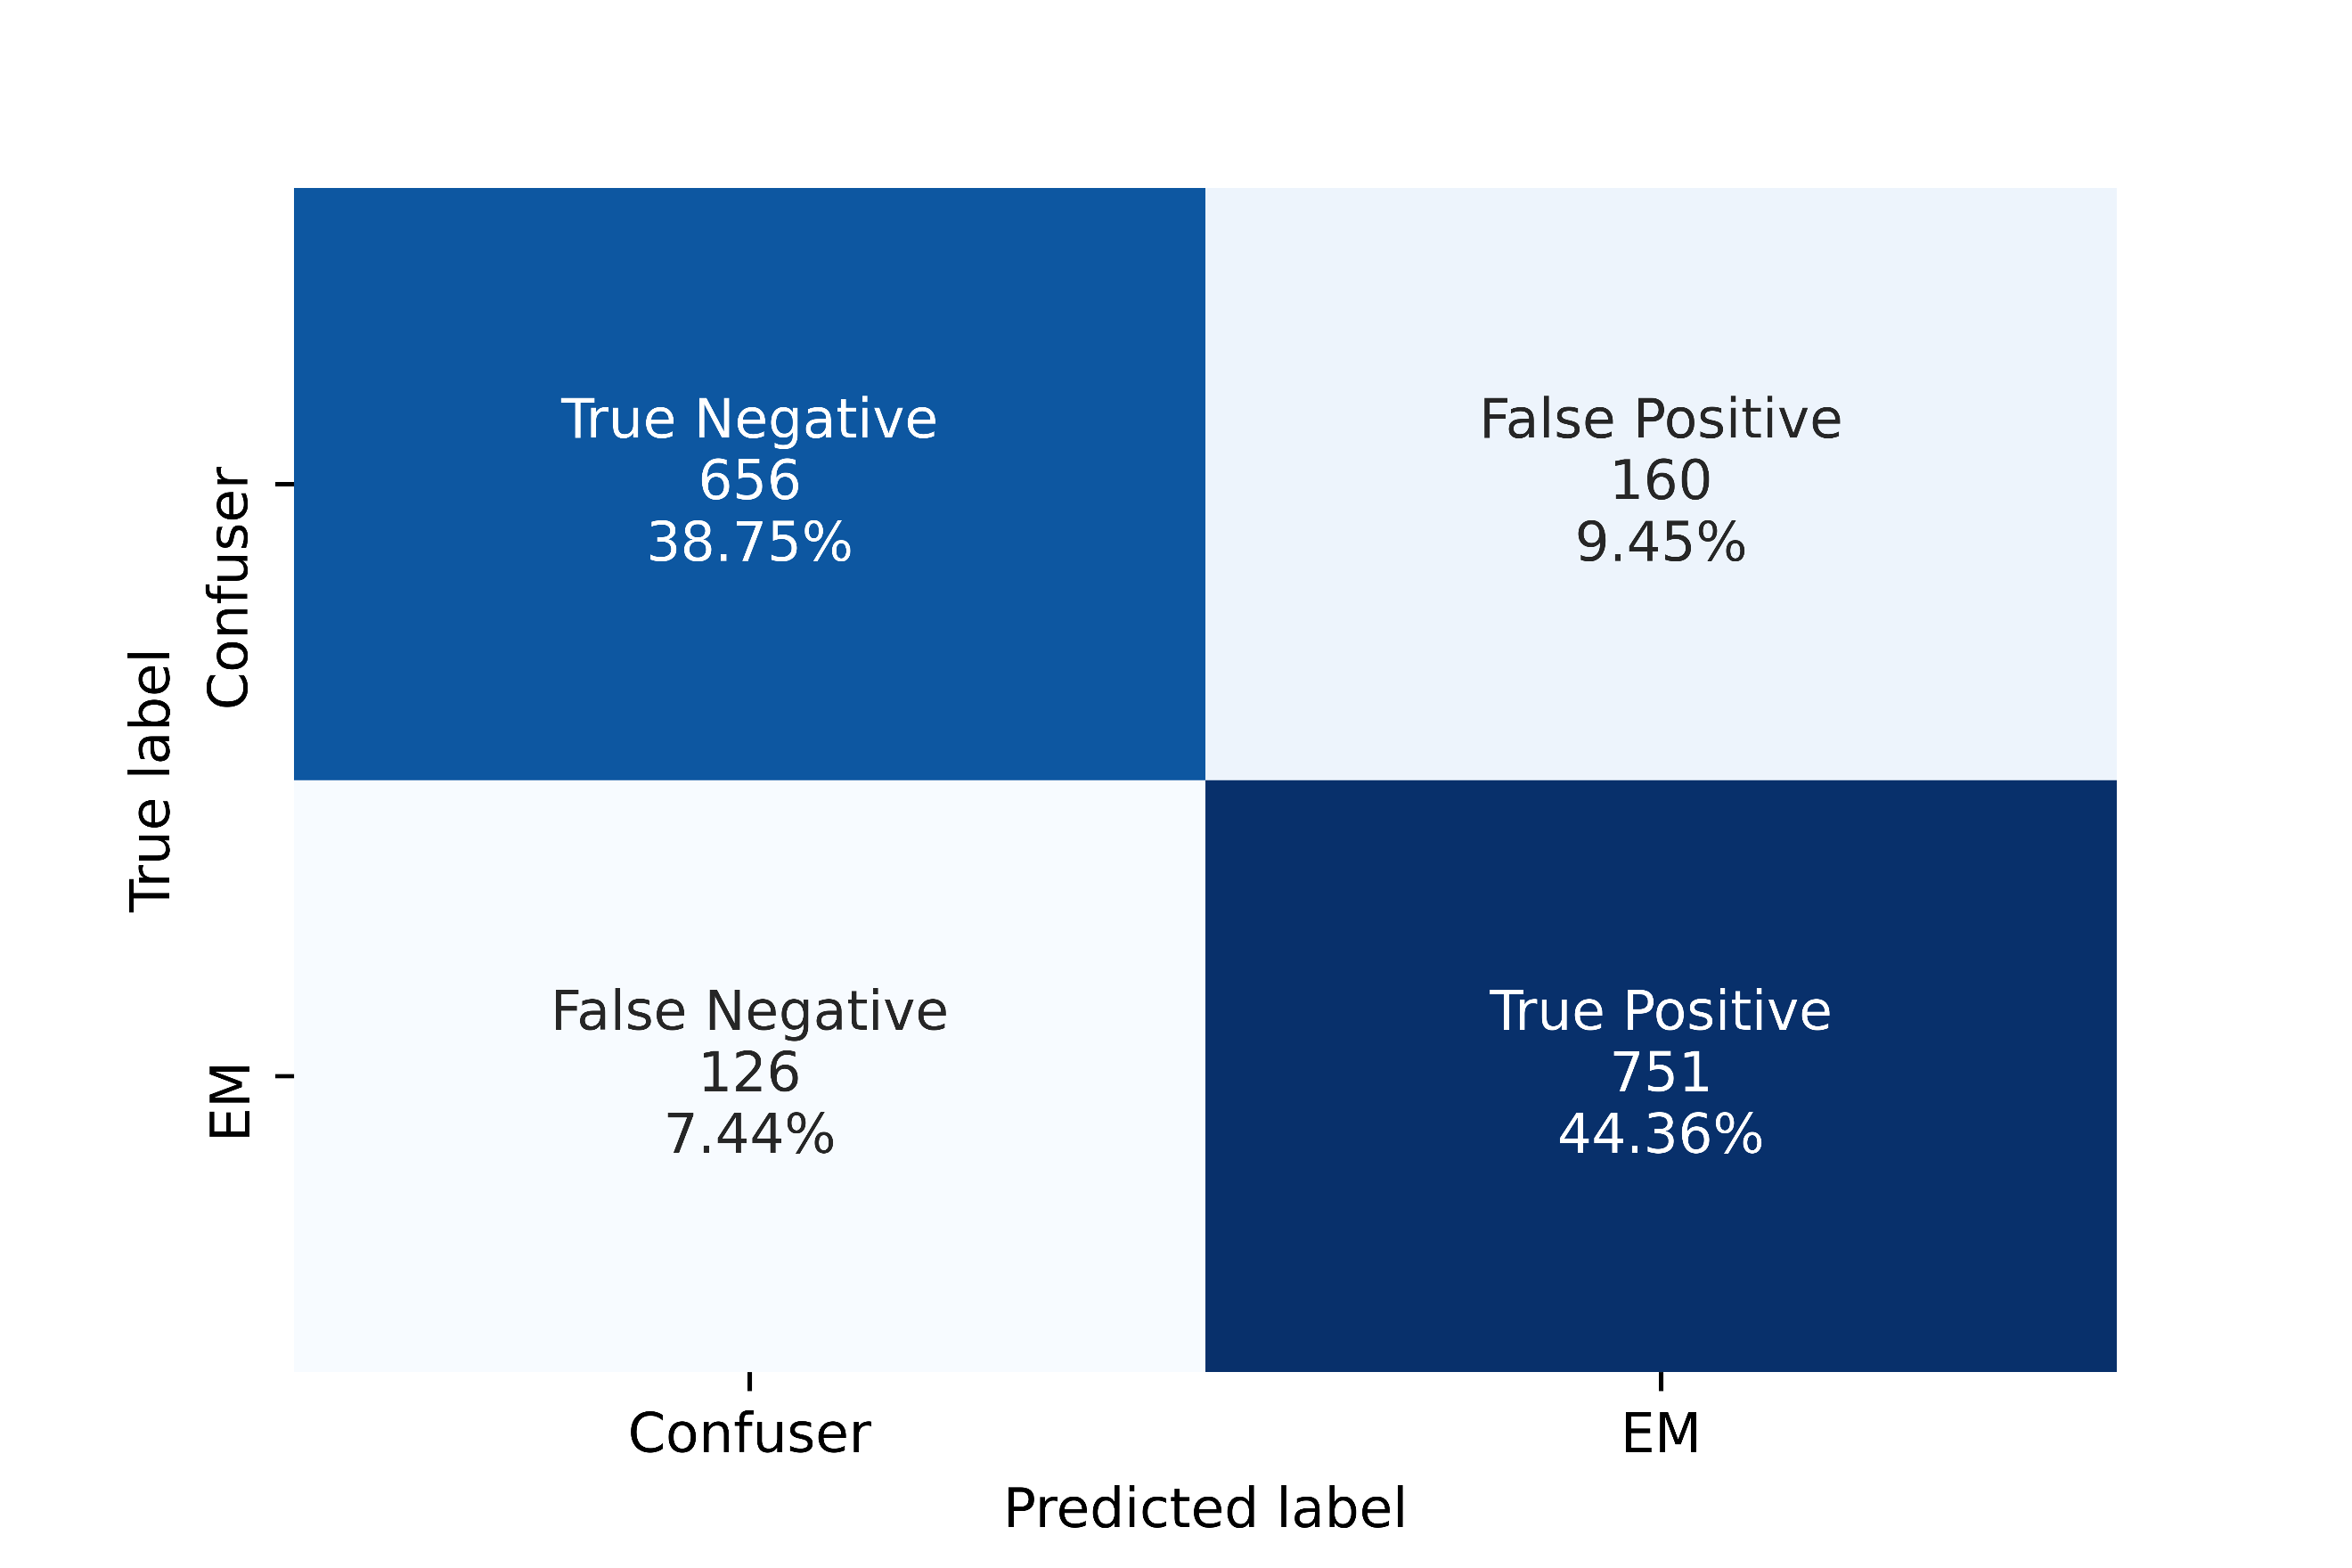
\includegraphics[width=\textwidth,keepaspectratio]{images/Supplement4/image142.png}
		\caption{Confusion matrix.}
	\end{subfigure}
	\caption{Five-fold cross-validation ROC curve and confusion matrix of DenseNet201-561 model.}
\end{figure}

%%%%%%%%%%%%%%Break%%%%%%%%%%%%%%%%%%%%%%
\vfill\clearpage
\subsection{MobileNetV2-62}

\begin{table}[h!]
	\centering
	\caption{Five-fold cross-validation performance metrics of MobileNetV2-62 model.}
	\resizebox{\textwidth}{!}{%
		\begin{tabular}{llllllllllll}
			\toprule
			& \multicolumn{11}{c}{\textbf{Metric}}    \\ \cmidrule(lr){2-12} 
			\multicolumn{1}{l}{\textbf{Fold}} & \rotatebox{45}{Accuracy} & 
			\rotatebox{45}{Sensitivity} & \rotatebox{45}{Specificity} & 
			\rotatebox{45}{Precision} & \rotatebox{45}{NPV} & \rotatebox{45}{MCC} & 
			\rotatebox{45}{Kappa} & \rotatebox{45}{LR$+$} & \rotatebox{45}{LR$-$} & 
			\rotatebox{45}{F1-Score} & \rotatebox{45}{AUC}  \\ \midrule
			fold1          & 78.09 & 76.76 & 79.53 & 80.23 & 75.98 & 0.5625 & 0.5619 & 3.7501 & 0.2922 & 0.7845 & 0.8705 \\
			fold2          & 81.79 & 80.35 & 83.33 & 83.73 & 79.88 & 0.6365 & 0.6359 & 4.8208 & 0.2358 & 0.8201 & 0.9074 \\
			fold3          & 83.53 & 86.13 & 80.75 & 82.78 & 84.42 & 0.6703 & 0.6697 & 4.4731 & 0.1718 & 0.8442 & 0.9025 \\
			fold4          & 83.53 & 85.55 & 81.37 & 83.15 & 83.97 & 0.6702 & 0.6699 & 4.5911 & 0.1776 & 0.8433 & 0.9006 \\
			fold5          & 81.44 & 80.92 & 81.99 & 82.84 & 80    & 0.6288 & 0.6286 & 4.4927 & 0.2327 & 0.8187 & 0.8856 \\\cmidrule(lr){1-12}
			average        & 81.68 & 81.94 & 81.39 & 82.55 & 80.85 & 0.6337 & 0.6332 & 4.4256 & 0.222  & 0.8222 & 0.8933 \\
			std. deviation & 1.99  & 3.49  & 1.26  & 1.21  & 3.09  & 0.0394 & 0.0395 & 0.3596 & 0.0441 & 0.0218 & 0.0135\\
			\bottomrule
		\end{tabular}%
	}
\end{table}


\begin{figure}[h!]
	\centering
	\begin{subfigure}[b]{0.49\textwidth}
		\centering
		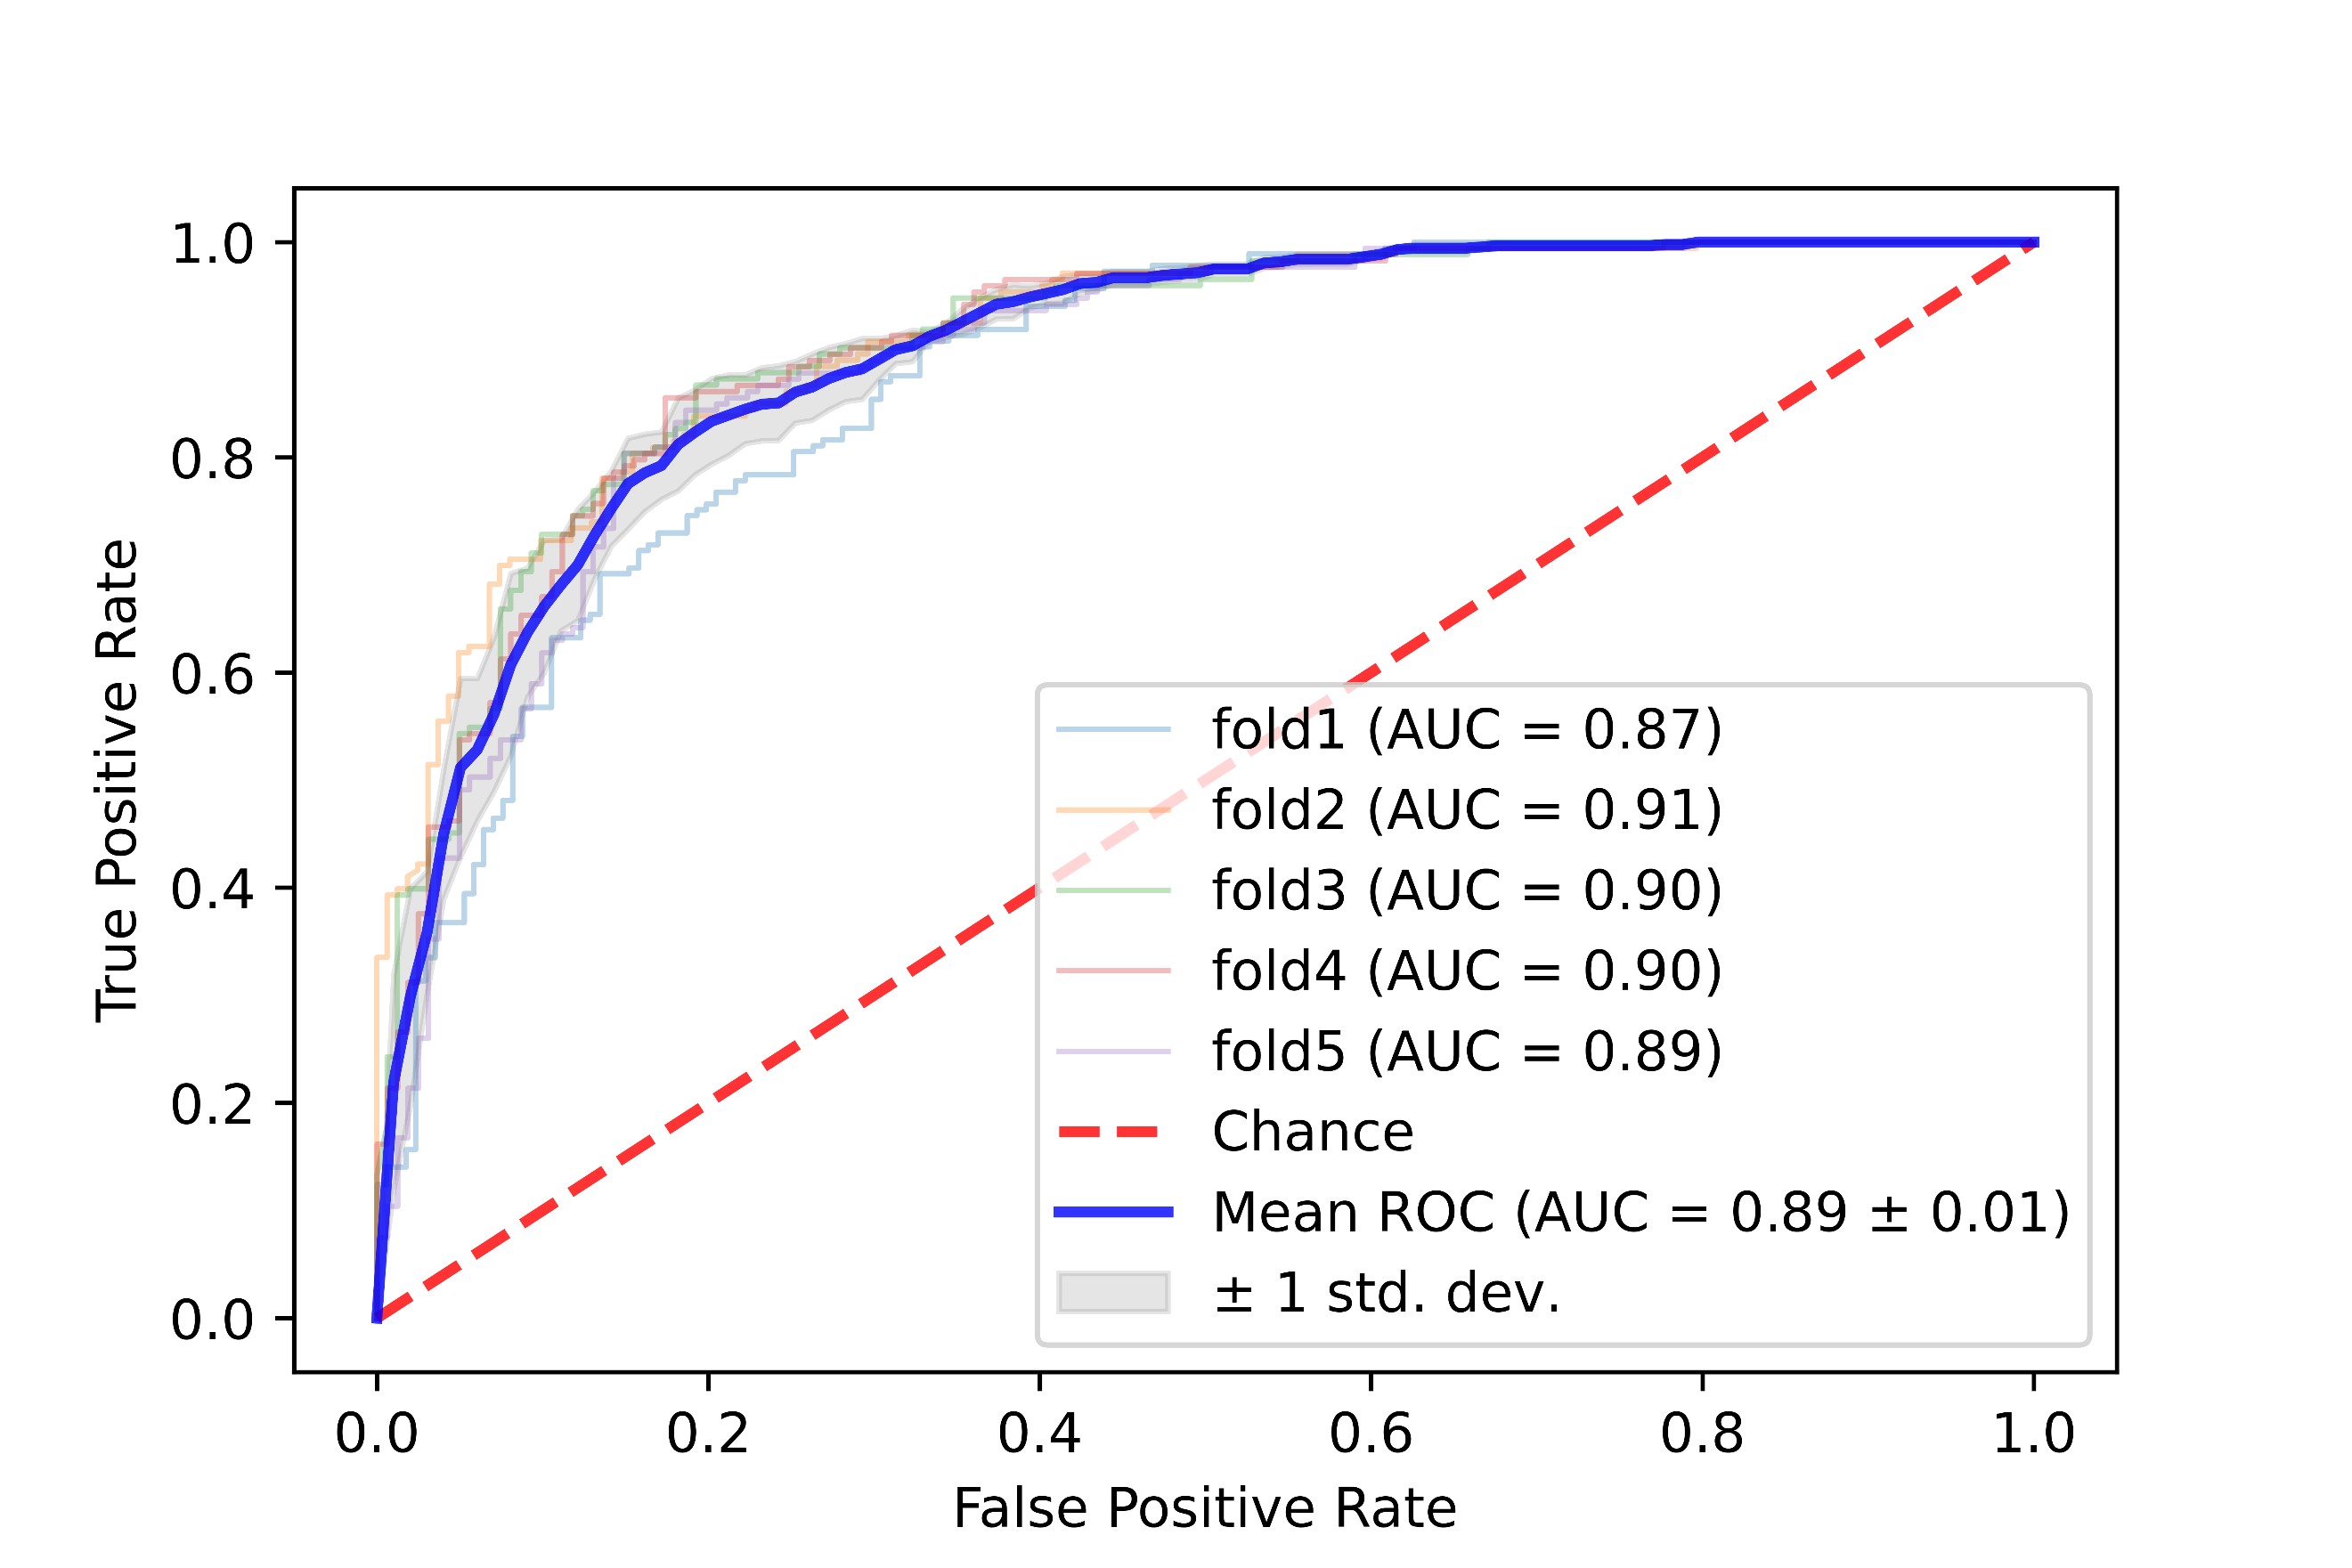
\includegraphics[width=\textwidth,keepaspectratio]{images/Supplement4/image143.png}
		\caption{ROC curve.}
	\end{subfigure}
	\hfill
	\begin{subfigure}[b]{0.49\textwidth}
		\centering
		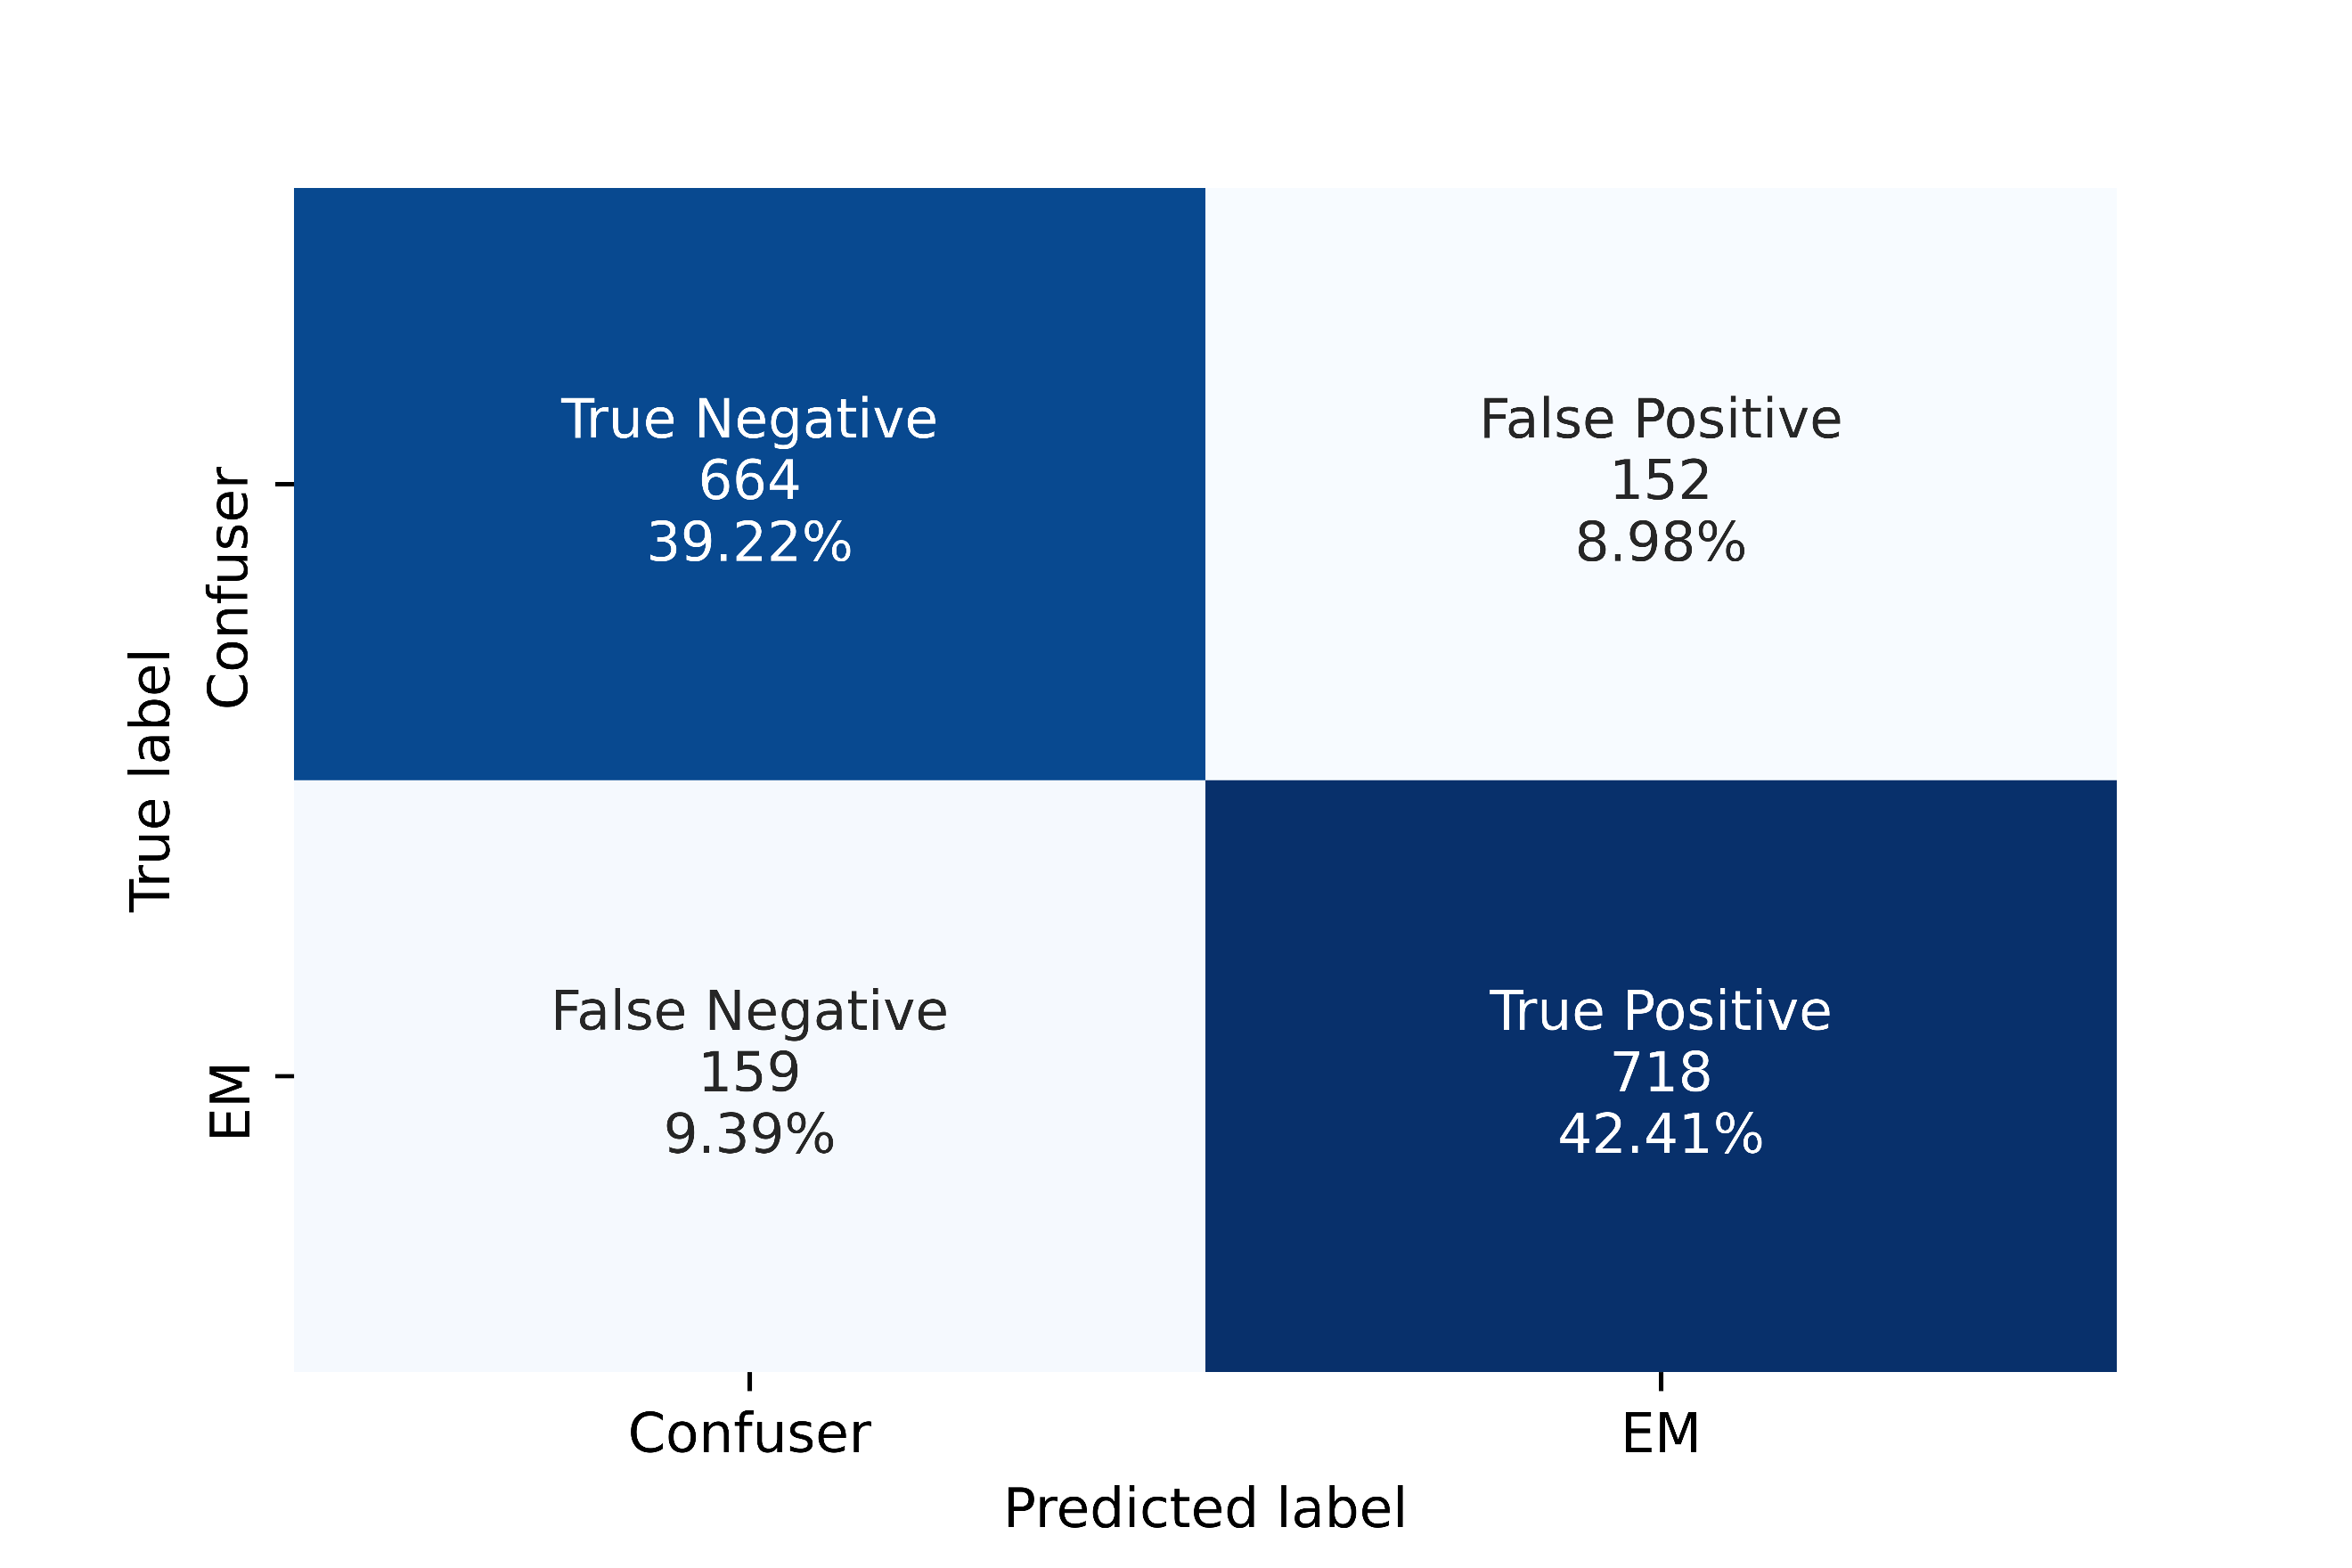
\includegraphics[width=\textwidth,keepaspectratio]{images/Supplement4/image149.png}
		\caption{Confusion matrix.}
	\end{subfigure}
	\caption{Five-fold cross-validation ROC curve and confusion matrix of MobileNetV2-62 model.}
\end{figure}

%%%%%%%%%%%%%%Break%%%%%%%%%%%%%%%%%%%%%%
\vfill\clearpage
\subsection{MobileNetV3Small-182}

\begin{table}[h!]
	\centering
	\caption{Five-fold cross-validation performance metrics of MobileNetV3Small-182 model.}
	\resizebox{\textwidth}{!}{%
		\begin{tabular}{llllllllllll}
			\toprule
			& \multicolumn{11}{c}{\textbf{Metric}}    \\ \cmidrule(lr){2-12} 
			\multicolumn{1}{l}{\textbf{Fold}} & \rotatebox{45}{Accuracy} & 
			\rotatebox{45}{Sensitivity} & \rotatebox{45}{Specificity} & 
			\rotatebox{45}{Precision} & \rotatebox{45}{NPV} & \rotatebox{45}{MCC} & 
			\rotatebox{45}{Kappa} & \rotatebox{45}{LR$+$} & \rotatebox{45}{LR$-$} & 
			\rotatebox{45}{F1-Score} & \rotatebox{45}{AUC}  \\ \midrule
			fold1          & 79.78 & 86.49 & 72.51 & 77.29 & 83.22 & 0.5975 & 0.5929 & 3.1466 & 0.1864 & 0.8163 & 0.8898 \\
			fold2          & 81.49 & 79.77 & 83.33 & 83.64 & 79.41 & 0.6308 & 0.63   & 4.7861 & 0.2428 & 0.8166 & 0.8887 \\
			fold3          & 79.04 & 83.24 & 74.53 & 77.84 & 80.54 & 0.5807 & 0.5792 & 3.2686 & 0.2249 & 0.8045 & 0.8805 \\
			fold4          & 84.43 & 89.6  & 78.88 & 82.01 & 87.59 & 0.6903 & 0.6871 & 4.2426 & 0.1319 & 0.8564 & 0.917  \\
			fold5          & 82.93 & 85.55 & 80.12 & 82.22 & 83.77 & 0.6583 & 0.6577 & 4.3042 & 0.1804 & 0.8385 & 0.9041 \\\cmidrule(lr){1-12}
			average        & 81.53 & 84.93 & 77.87 & 80.6  & 82.91 & 0.6315 & 0.6294 & 3.9496 & 0.1933 & 0.8265 & 0.896  \\
			std. deviation & 1.98  & 3.29  & 3.89  & 2.55  & 2.85  & 0.0398 & 0.04   & 0.6356 & 0.0386 & 0.0186 & 0.013 \\
			\bottomrule
		\end{tabular}%
	}
\end{table}


\begin{figure}[h!]
	\centering
	\begin{subfigure}[b]{0.49\textwidth}
		\centering
		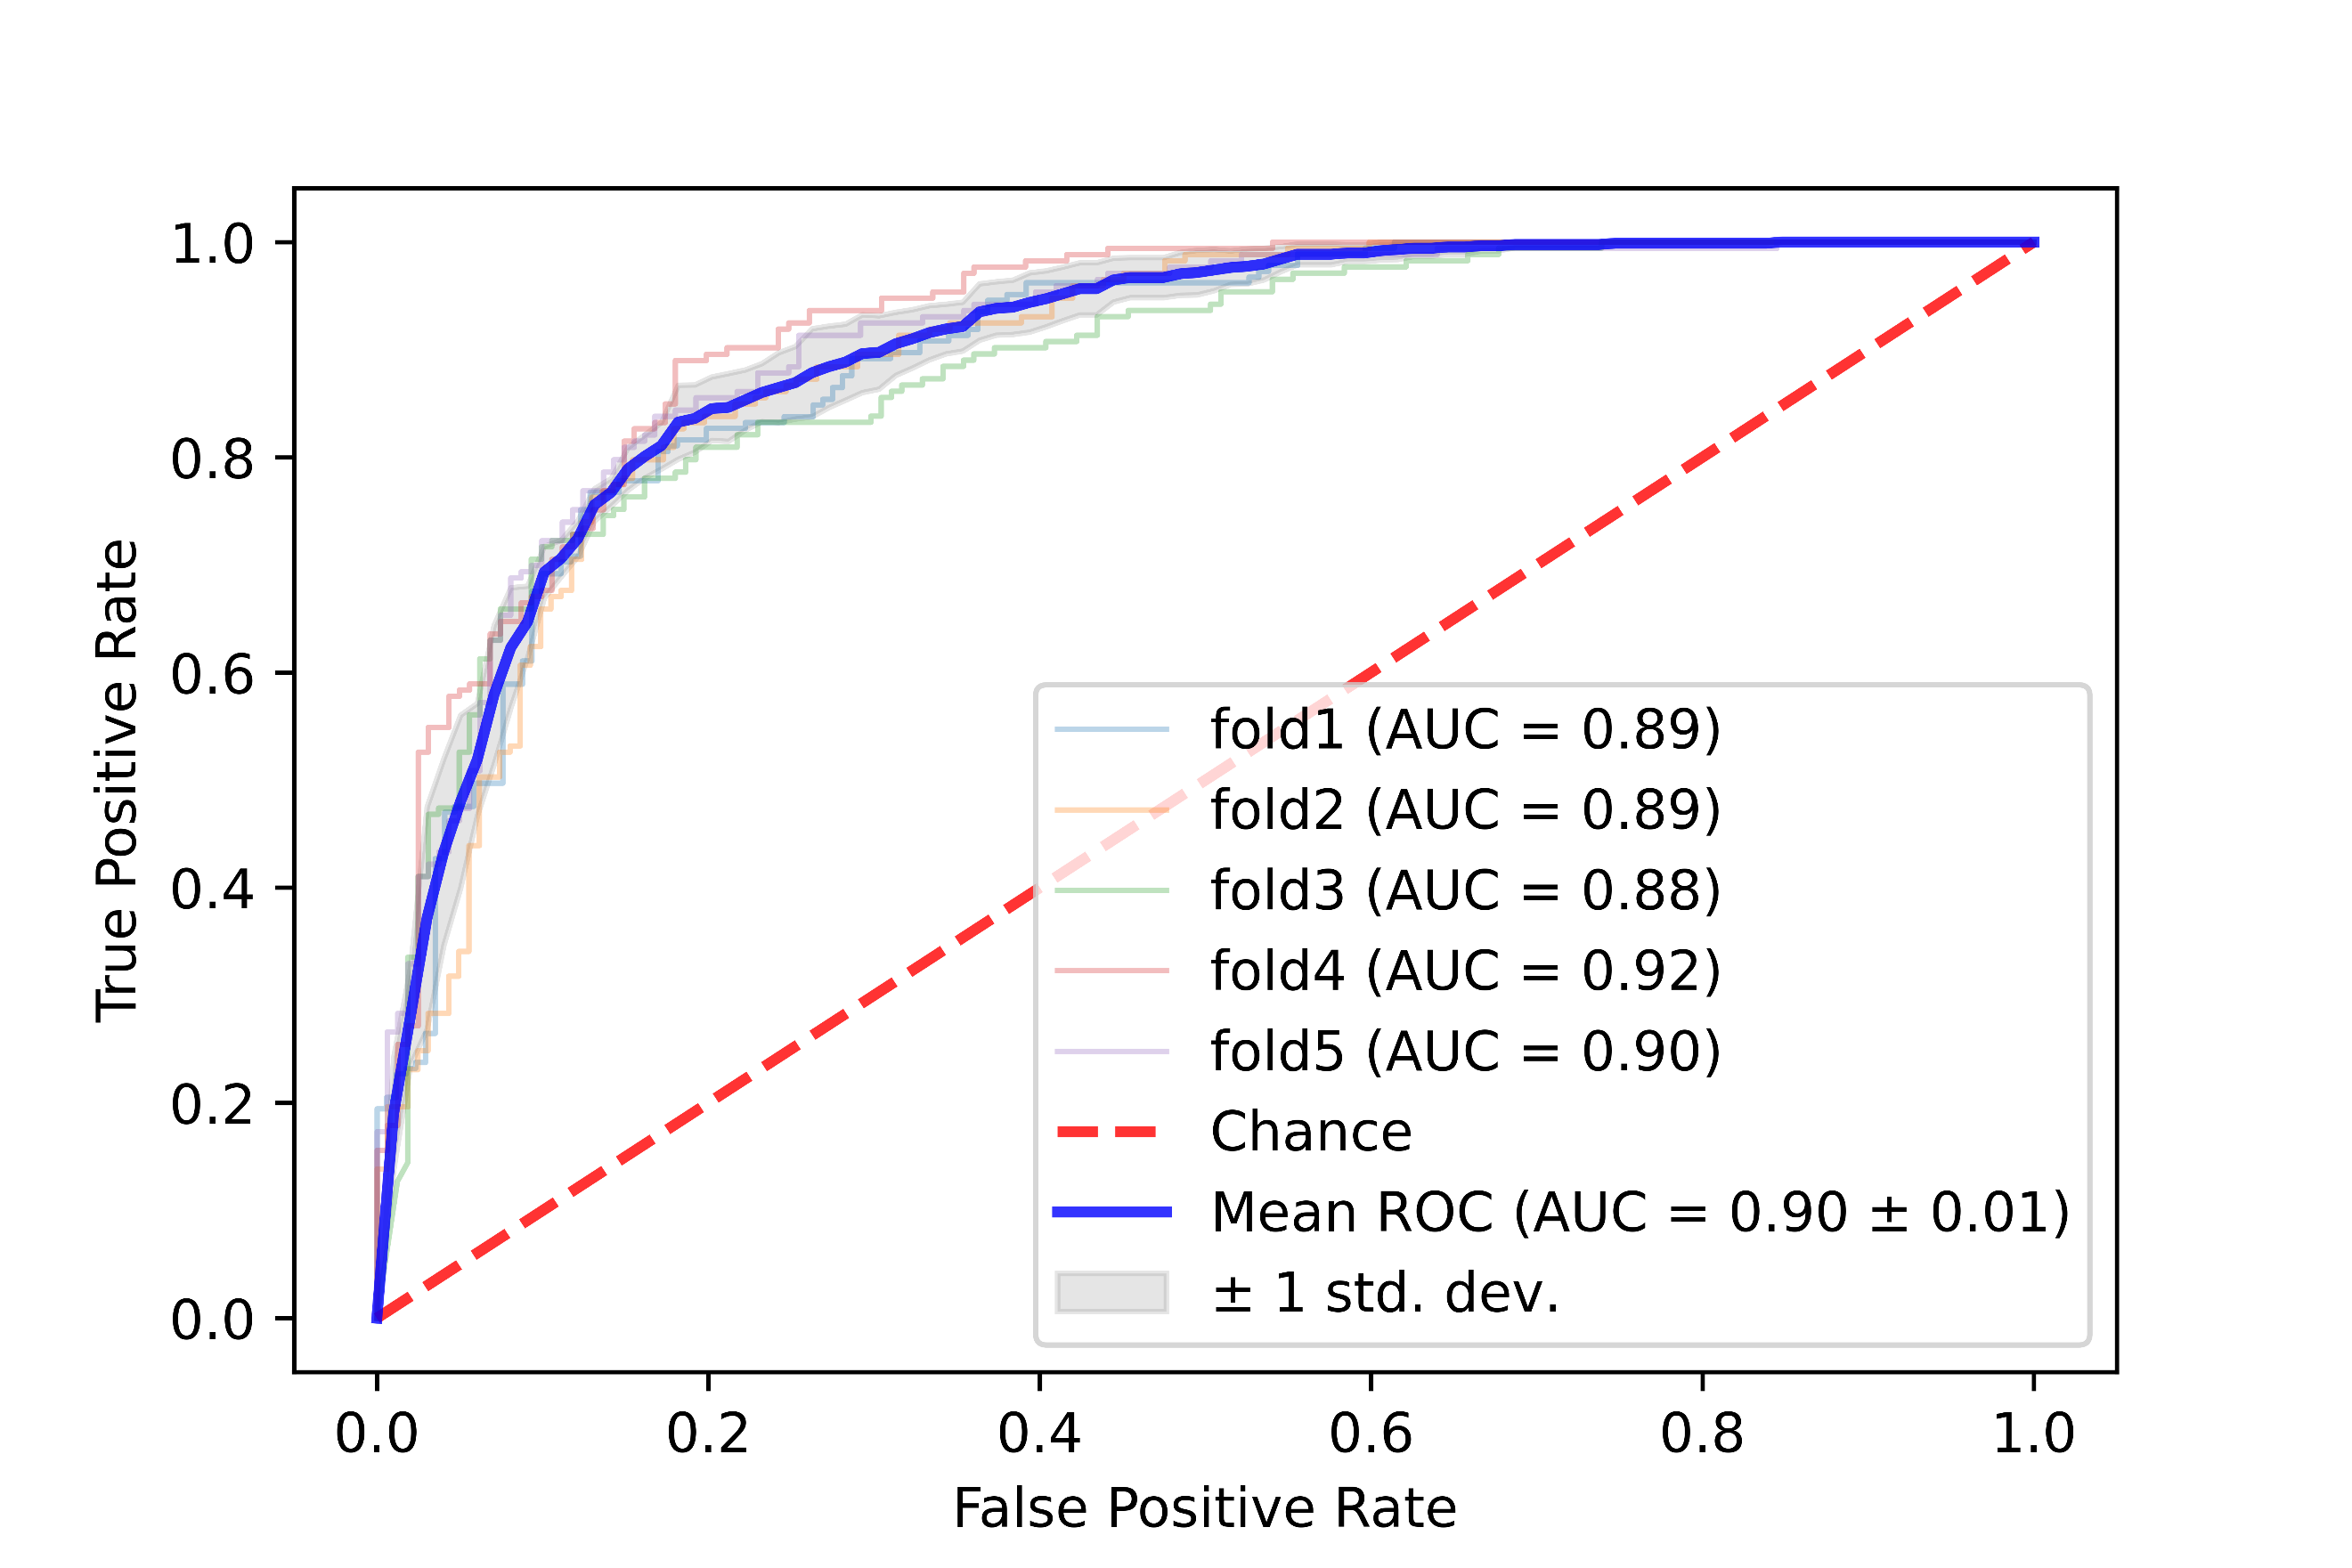
\includegraphics[width=\textwidth,keepaspectratio]{images/Supplement4/image150.png}
		\caption{ROC curve.}
	\end{subfigure}
	\hfill
	\begin{subfigure}[b]{0.49\textwidth}
		\centering
		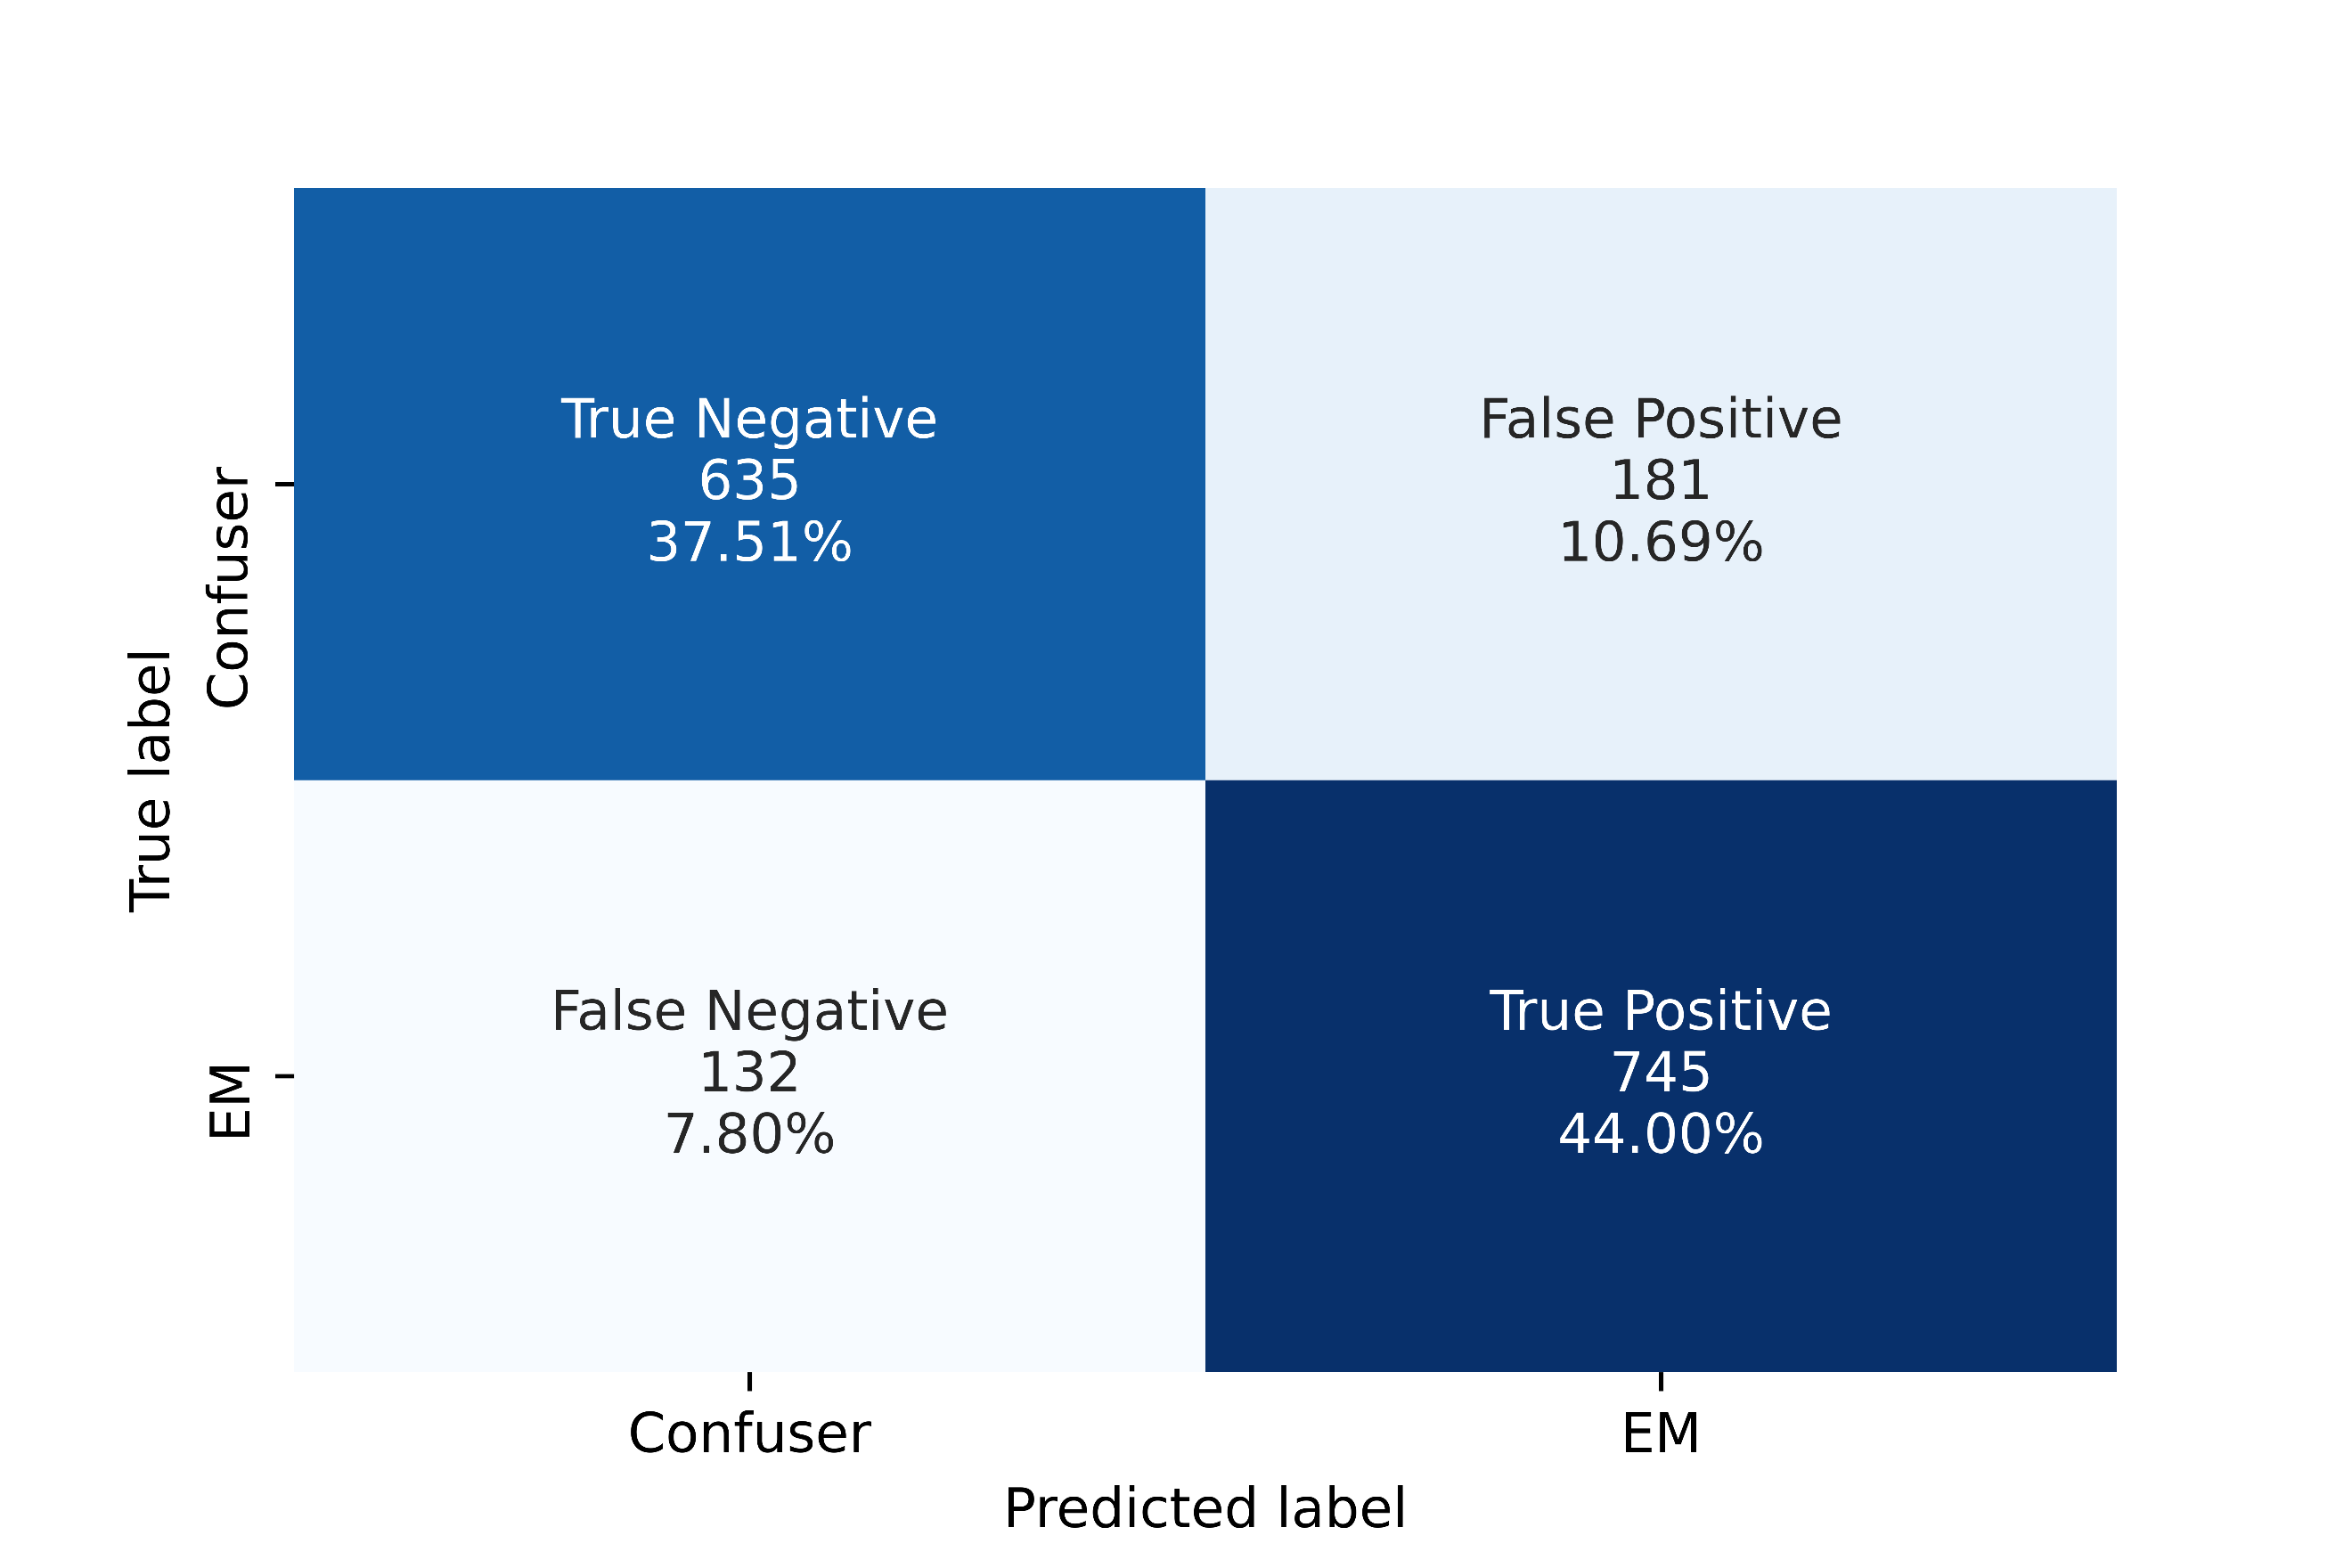
\includegraphics[width=\textwidth,keepaspectratio]{images/Supplement4/image156.png}
		\caption{Confusion matrix.}
	\end{subfigure}
	\caption{Five-fold cross-validation ROC curve and confusion matrix of MobileNetV3Small-182 model.}
\end{figure}

%%%%%%%%%%%%%%Break%%%%%%%%%%%%%%%%%%%%%%
\vfill\clearpage
\subsection{MobileNetV3Large-193}

\begin{table}[h!]
	\centering
	\caption{Five-fold cross-validation performance metrics of MobileNetV3Large-193 model.}
	\resizebox{\textwidth}{!}{%
		\begin{tabular}{llllllllllll}
			\toprule
			& \multicolumn{11}{c}{\textbf{Metric}}    \\ \cmidrule(lr){2-12} 
			\multicolumn{1}{l}{\textbf{Fold}} & \rotatebox{45}{Accuracy} & 
			\rotatebox{45}{Sensitivity} & \rotatebox{45}{Specificity} & 
			\rotatebox{45}{Precision} & \rotatebox{45}{NPV} & \rotatebox{45}{MCC} & 
			\rotatebox{45}{Kappa} & \rotatebox{45}{LR$+$} & \rotatebox{45}{LR$-$} & 
			\rotatebox{45}{F1-Score} & \rotatebox{45}{AUC}  \\ \midrule
			fold1          & 78.93 & 83.78 & 73.68 & 77.5  & 80.77 & 0.5787 & 0.5766 & 3.1838 & 0.2201 & 0.8052 & 0.8884 \\
			fold2          & 83.58 & 83.24 & 83.95 & 84.71 & 82.42 & 0.6716 & 0.6715 & 5.1863 & 0.1997 & 0.8397 & 0.9092 \\
			fold3          & 82.93 & 83.24 & 82.61 & 83.72 & 82.1  & 0.6583 & 0.6583 & 4.7861 & 0.2029 & 0.8348 & 0.8973 \\
			fold4          & 82.63 & 84.39 & 80.75 & 82.49 & 82.8  & 0.6521 & 0.6519 & 4.383  & 0.1933 & 0.8343 & 0.9073 \\
			fold5          & 85.63 & 83.82 & 87.58 & 87.88 & 83.43 & 0.7135 & 0.7127 & 6.7471 & 0.1848 & 0.858  & 0.915  \\
			average        & 82.74 & 83.69 & 81.71 & 83.26 & 82.3  & 0.6548 & 0.6542 & 4.8573 & 0.2002 & 0.8344 & 0.9034 \\
			std. deviation & 2.17  & 0.43  & 4.6   & 3.39  & 0.89  & 0.0437 & 0.0442 & 1.1585 & 0.0117 & 0.017  & 0.0094 \\
			\bottomrule
		\end{tabular}%
	}
\end{table}


\begin{figure}[h!]
	\centering
	\begin{subfigure}[b]{0.49\textwidth}
		\centering
		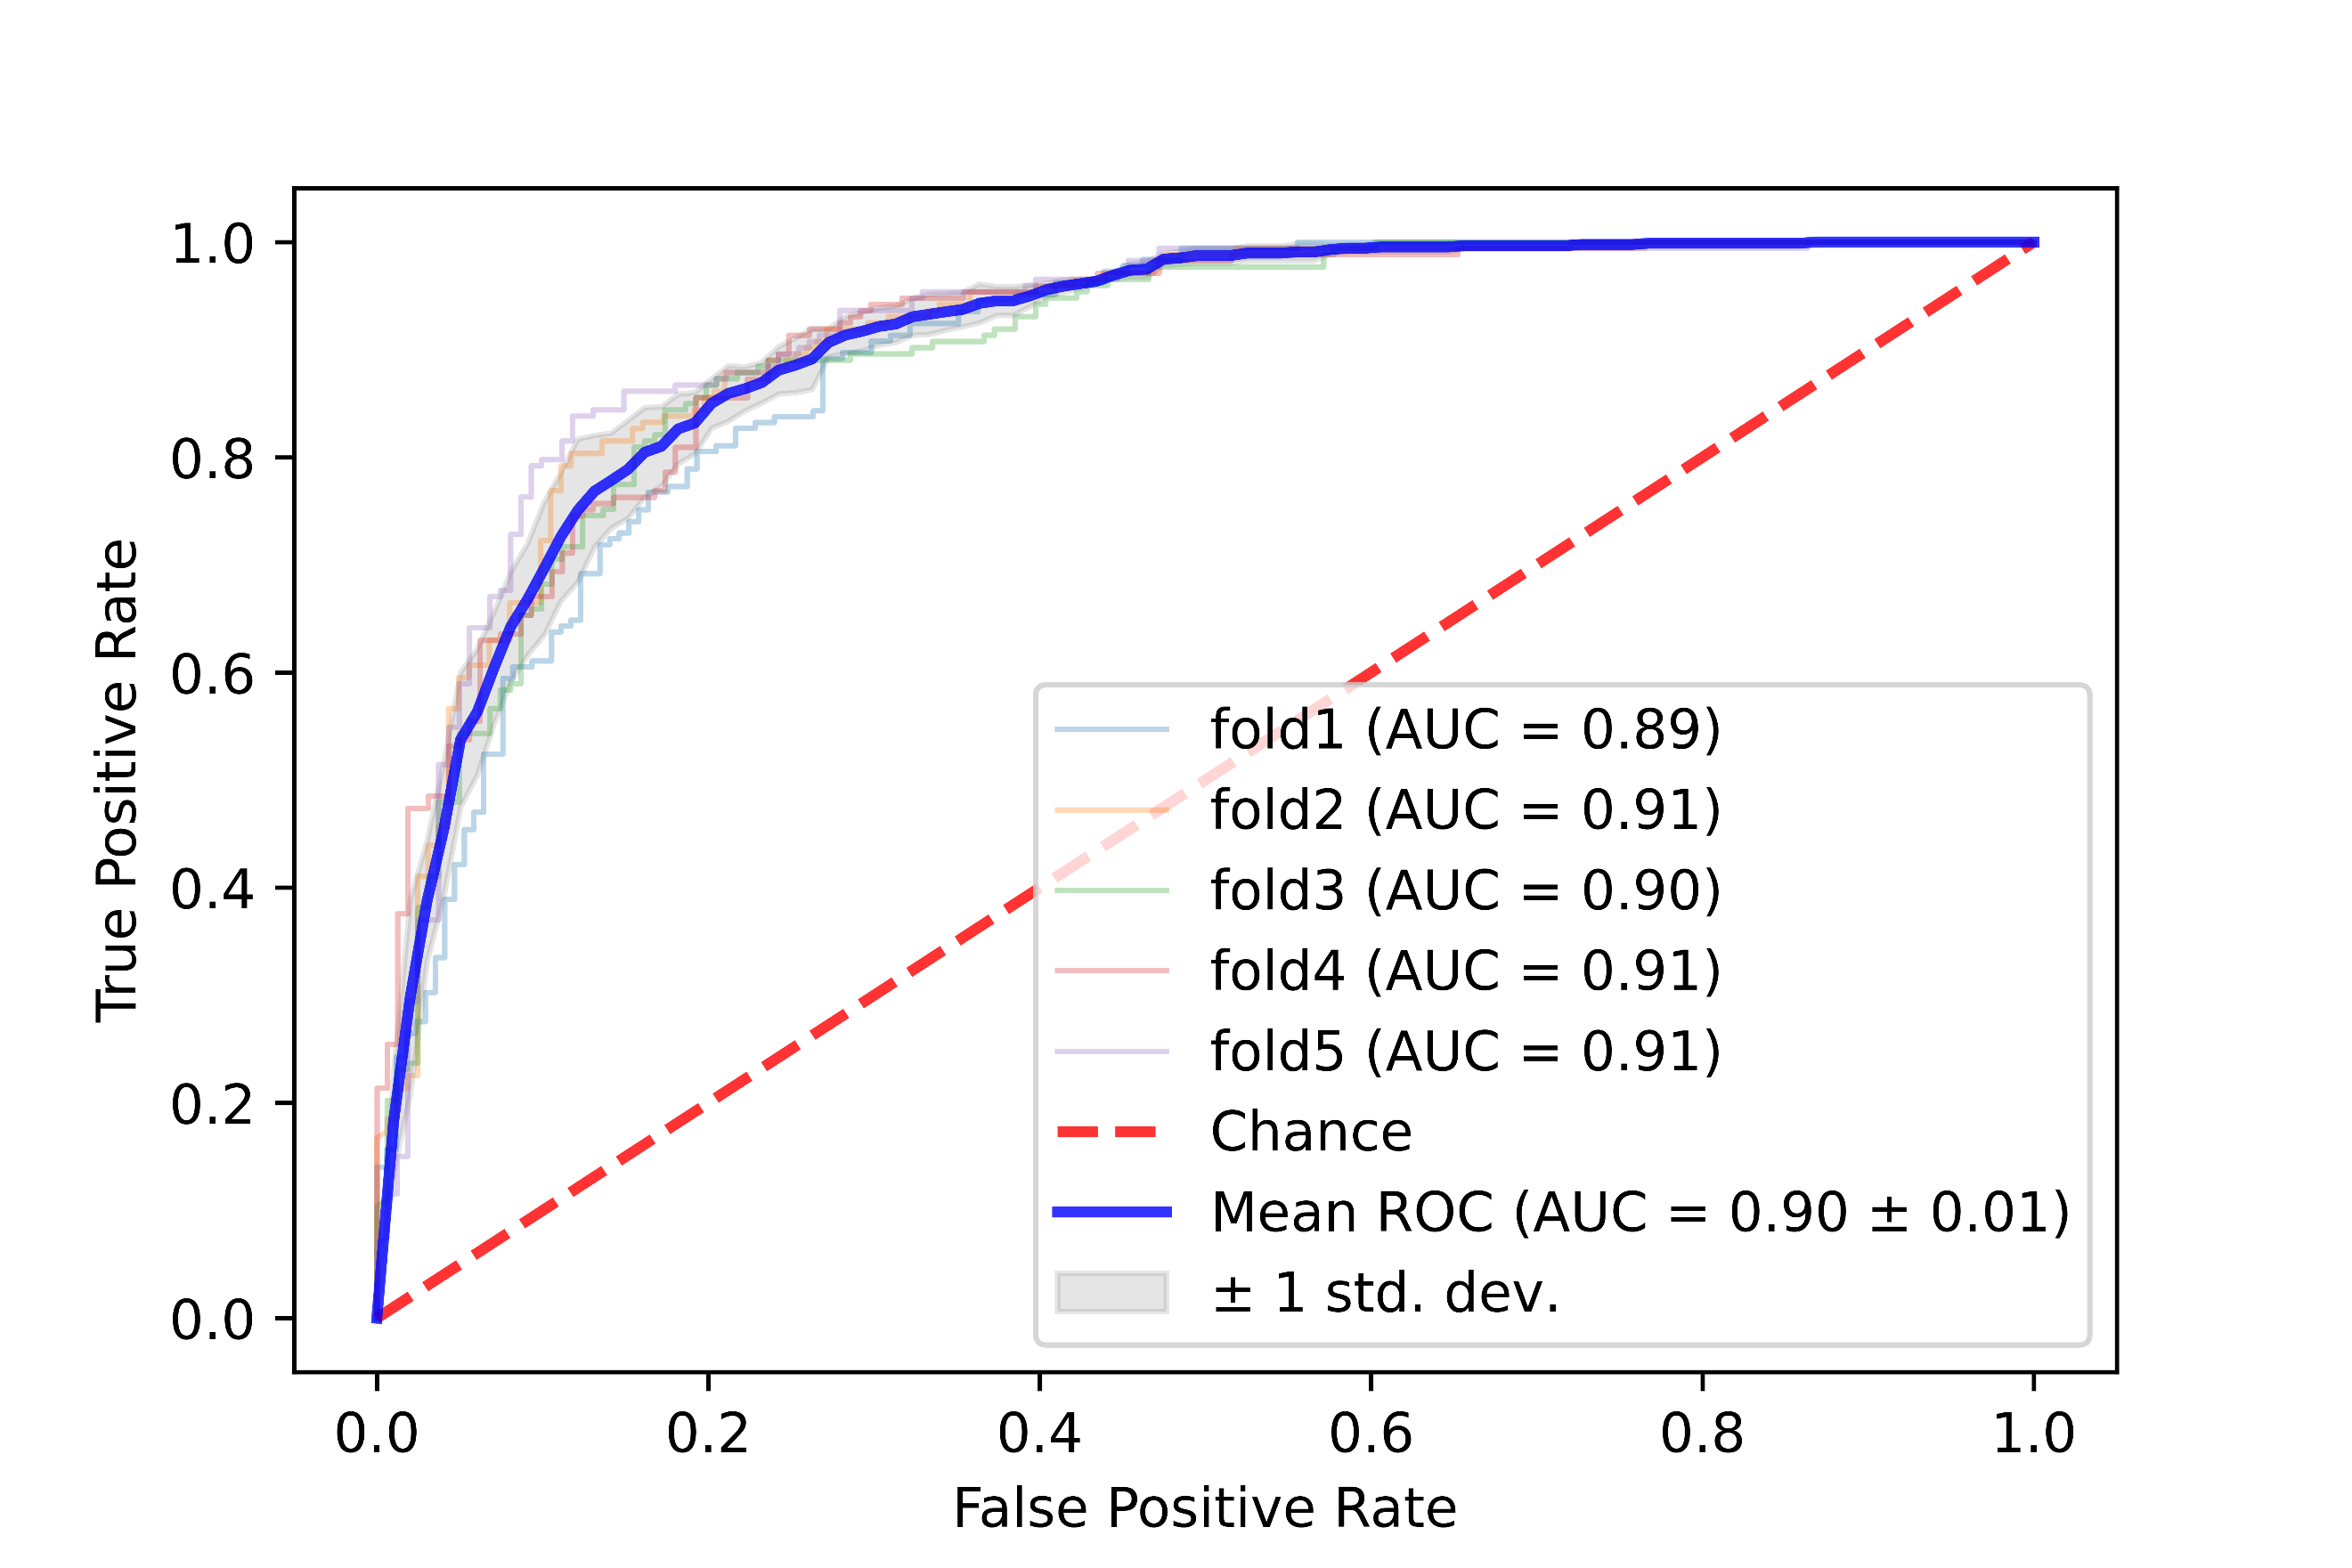
\includegraphics[width=\textwidth,keepaspectratio]{images/Supplement4/image157.png}
		\caption{ROC curve.}
	\end{subfigure}
	\hfill
	\begin{subfigure}[b]{0.49\textwidth}
		\centering
		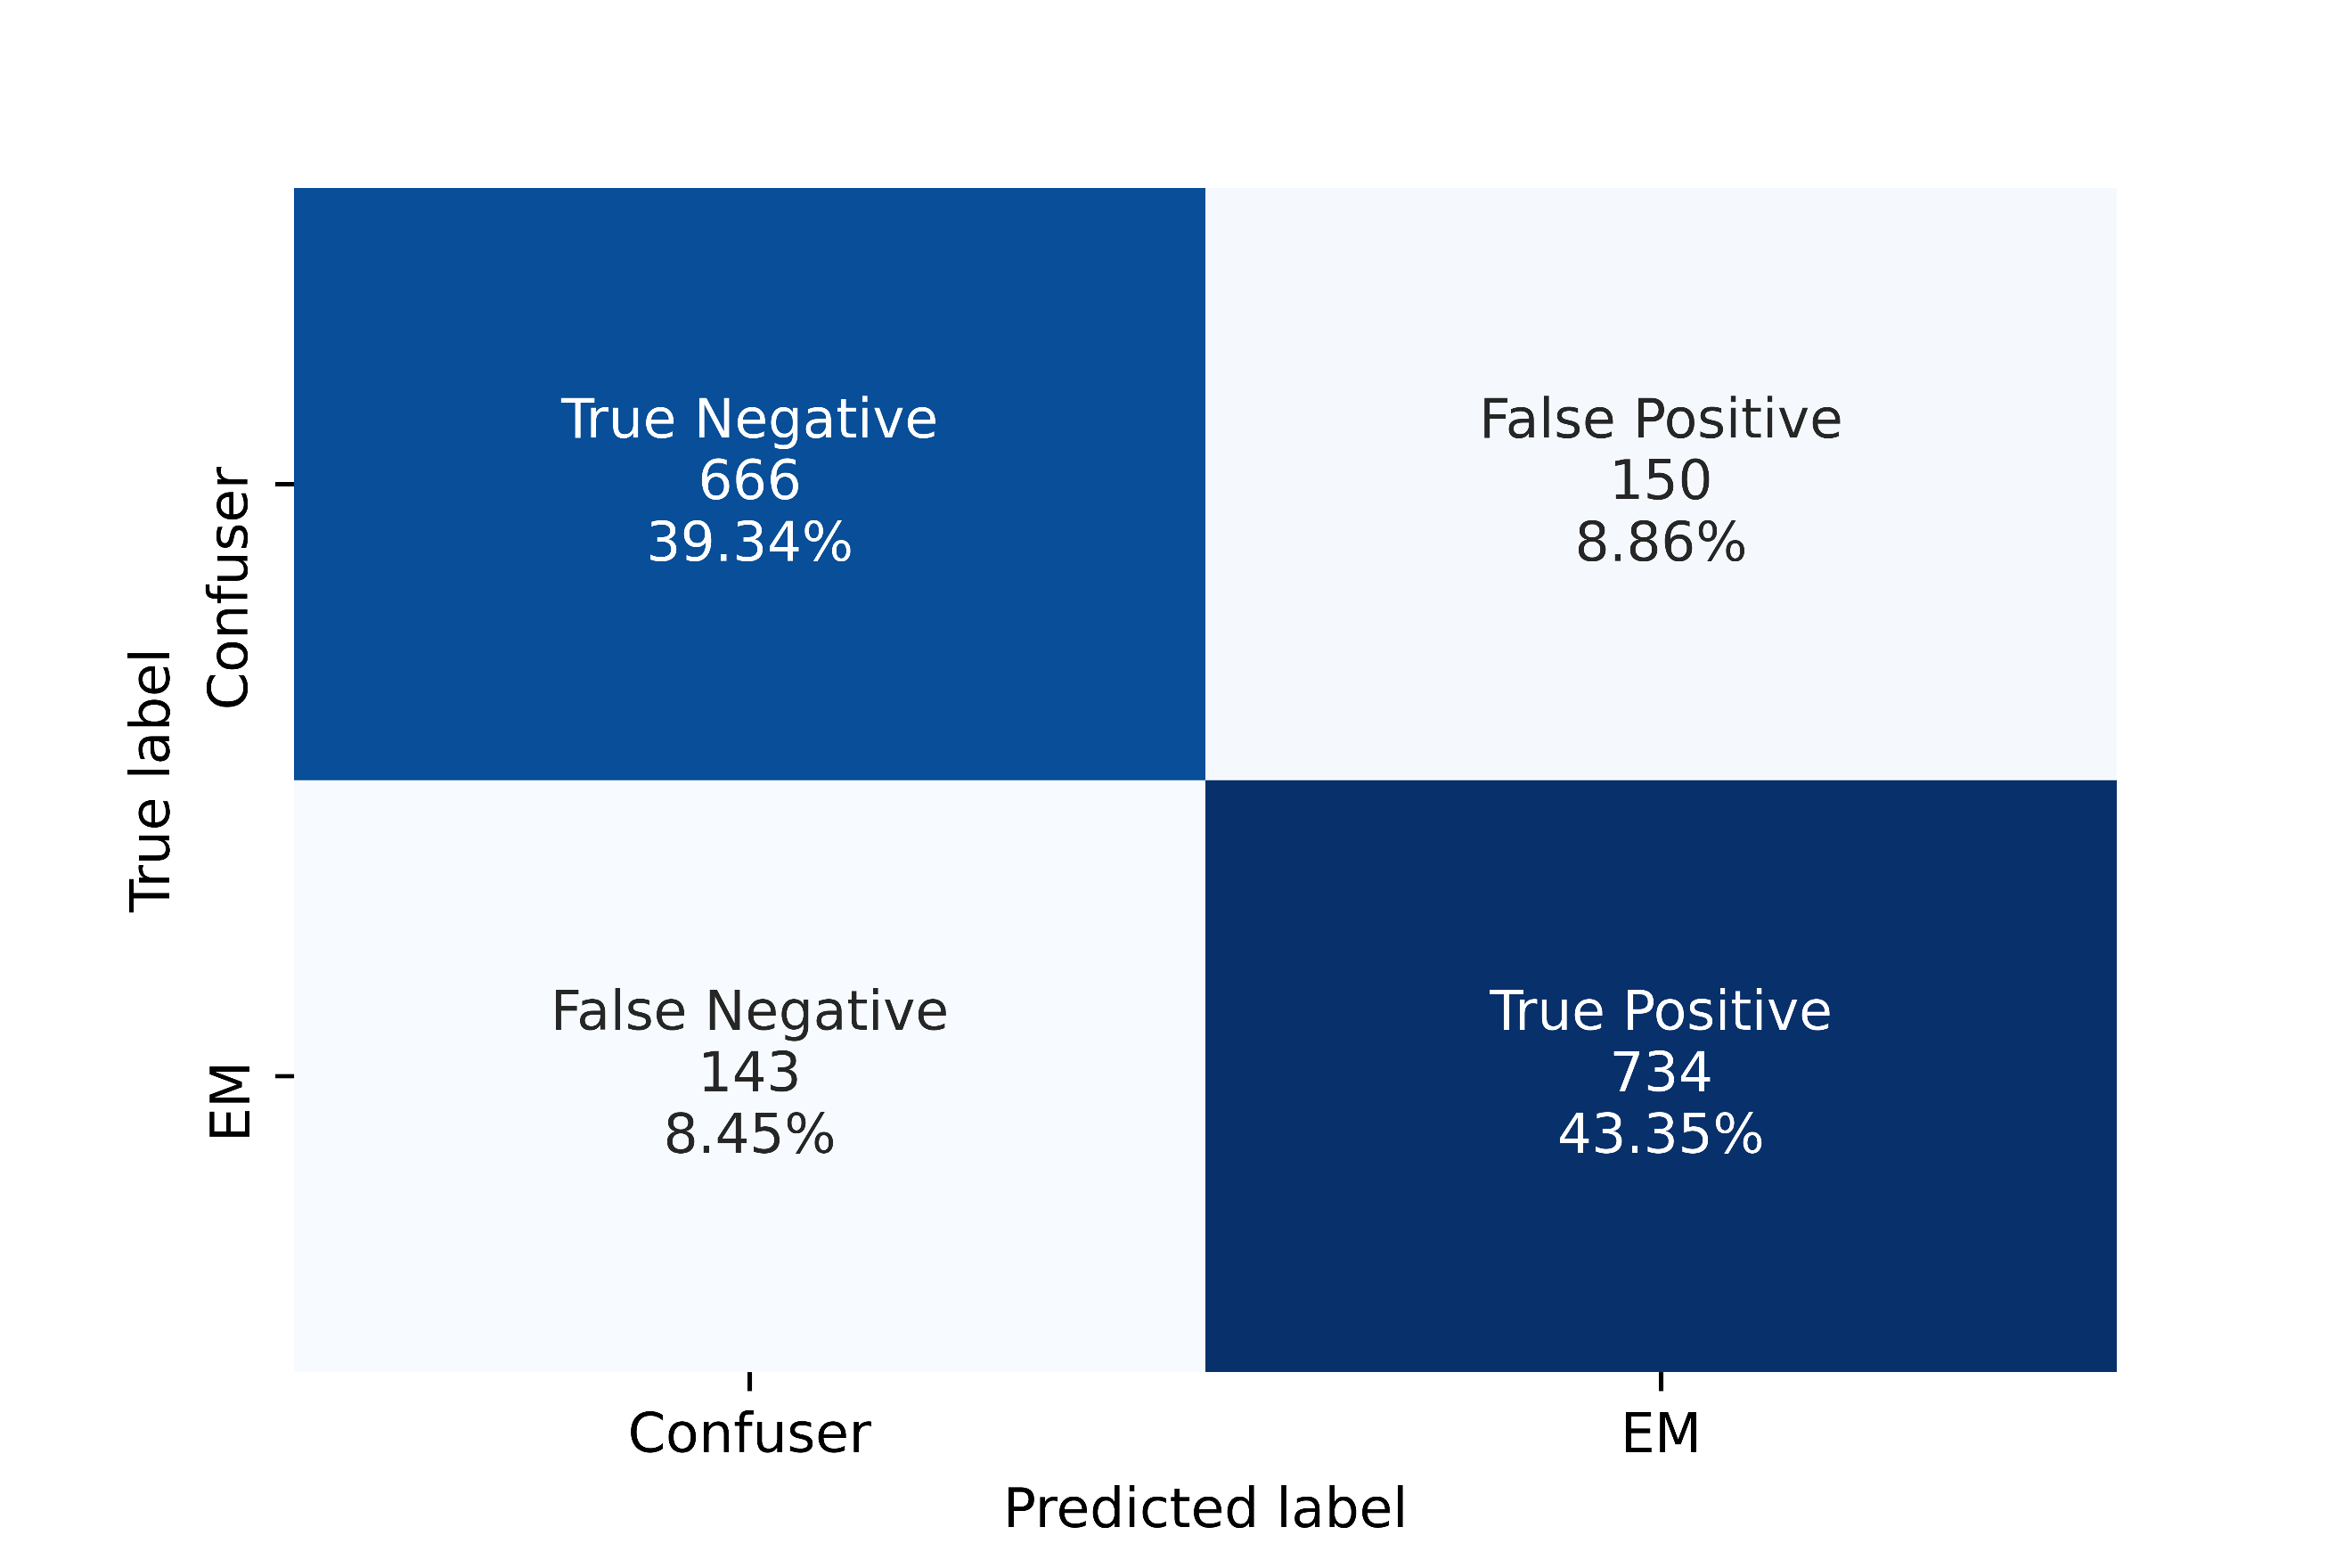
\includegraphics[width=\textwidth,keepaspectratio]{images/Supplement4/image162.png}
		\caption{Confusion matrix.}
	\end{subfigure}
	\caption{Five-fold cross-validation ROC curve and confusion matrix of MobileNetV3Large-193 model.}
\end{figure}

%%%%%%%%%%%%%%Break%%%%%%%%%%%%%%%%%%%%%%
\vfill\clearpage
\subsection{NASNetMobile-617}

\begin{table}[h!]
	\centering
	\caption{Five-fold cross-validation performance metrics of NASNetMobile-617 model.}
	\resizebox{\textwidth}{!}{%
		\begin{tabular}{llllllllllll}
			\toprule
			& \multicolumn{11}{c}{\textbf{Metric}}    \\ \cmidrule(lr){2-12} 
			\multicolumn{1}{l}{\textbf{Fold}} & \rotatebox{45}{Accuracy} & 
			\rotatebox{45}{Sensitivity} & \rotatebox{45}{Specificity} & 
			\rotatebox{45}{Precision} & \rotatebox{45}{NPV} & \rotatebox{45}{MCC} & 
			\rotatebox{45}{Kappa} & \rotatebox{45}{LR$+$} & \rotatebox{45}{LR$-$} & 
			\rotatebox{45}{F1-Score} & \rotatebox{45}{AUC}  \\ \midrule
			fold1          & 79.49 & 85.95 & 72.51 & 77.18 & 82.67 & 0.5915 & 0.5873 & 3.127  & 0.1938 & 0.8133 & 0.8665 \\
			fold2          & 80.3  & 82.66 & 77.78 & 79.89 & 80.77 & 0.6055 & 0.6051 & 3.7197 & 0.223  & 0.8125 & 0.8855 \\
			fold3          & 80.84 & 80.92 & 80.75 & 81.87 & 79.75 & 0.6165 & 0.6164 & 4.2029 & 0.2362 & 0.814  & 0.8836 \\
			fold4          & 82.34 & 83.82 & 80.75 & 82.39 & 82.28 & 0.6461 & 0.646  & 4.353  & 0.2004 & 0.8309 & 0.9055 \\
			fold5          & 83.53 & 82.66 & 84.47 & 85.12 & 81.93 & 0.6709 & 0.6706 & 5.3232 & 0.2053 & 0.8387 & 0.9072 \\\cmidrule(lr){1-12}
			average        & 81.3  & 83.2  & 79.25 & 81.29 & 81.48 & 0.6261 & 0.6251 & 4.1452 & 0.2117 & 0.8219 & 0.8897 \\
			std. deviation & 1.45  & 1.66  & 3.98  & 2.65  & 1.07  & 0.0287 & 0.0297 & 0.7283 & 0.0156 & 0.0108 & 0.0152\\
			\bottomrule
		\end{tabular}%
	}
\end{table}


\begin{figure}[h!]
	\centering
	\begin{subfigure}[b]{0.49\textwidth}
		\centering
		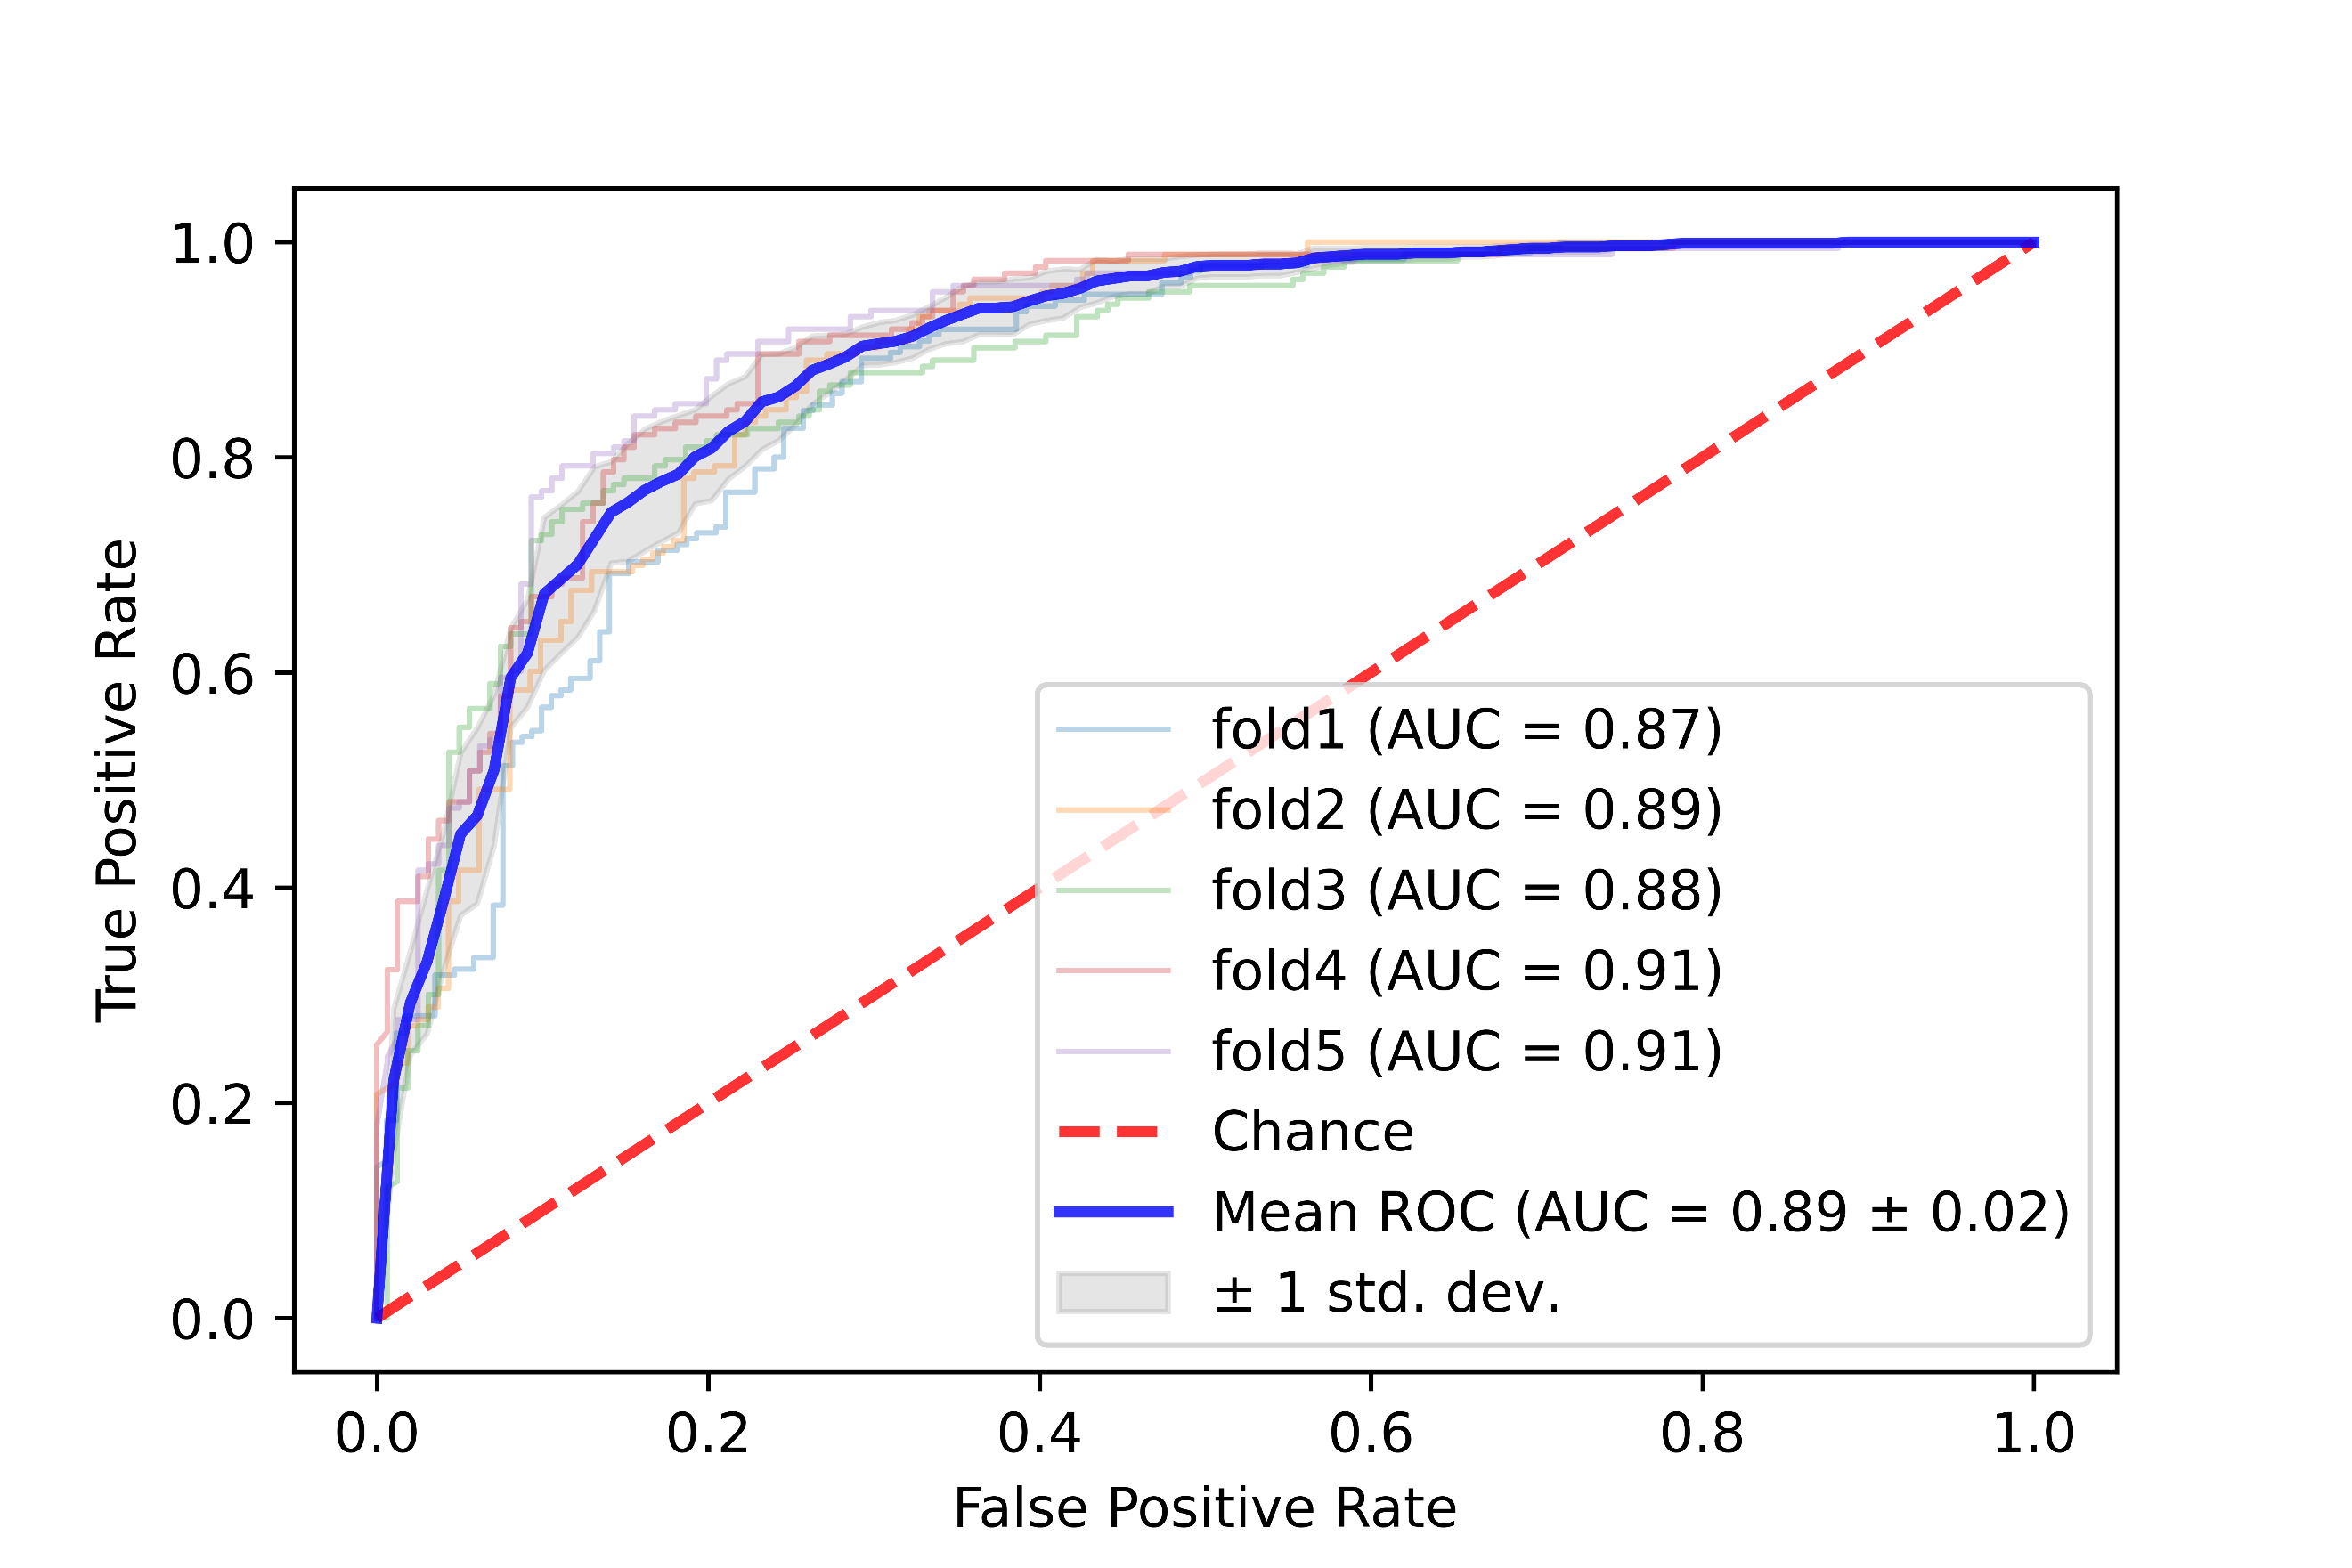
\includegraphics[width=\textwidth,keepaspectratio]{images/Supplement4/image163.png}
		\caption{ROC curve.}
	\end{subfigure}
	\hfill
	\begin{subfigure}[b]{0.49\textwidth}
		\centering
		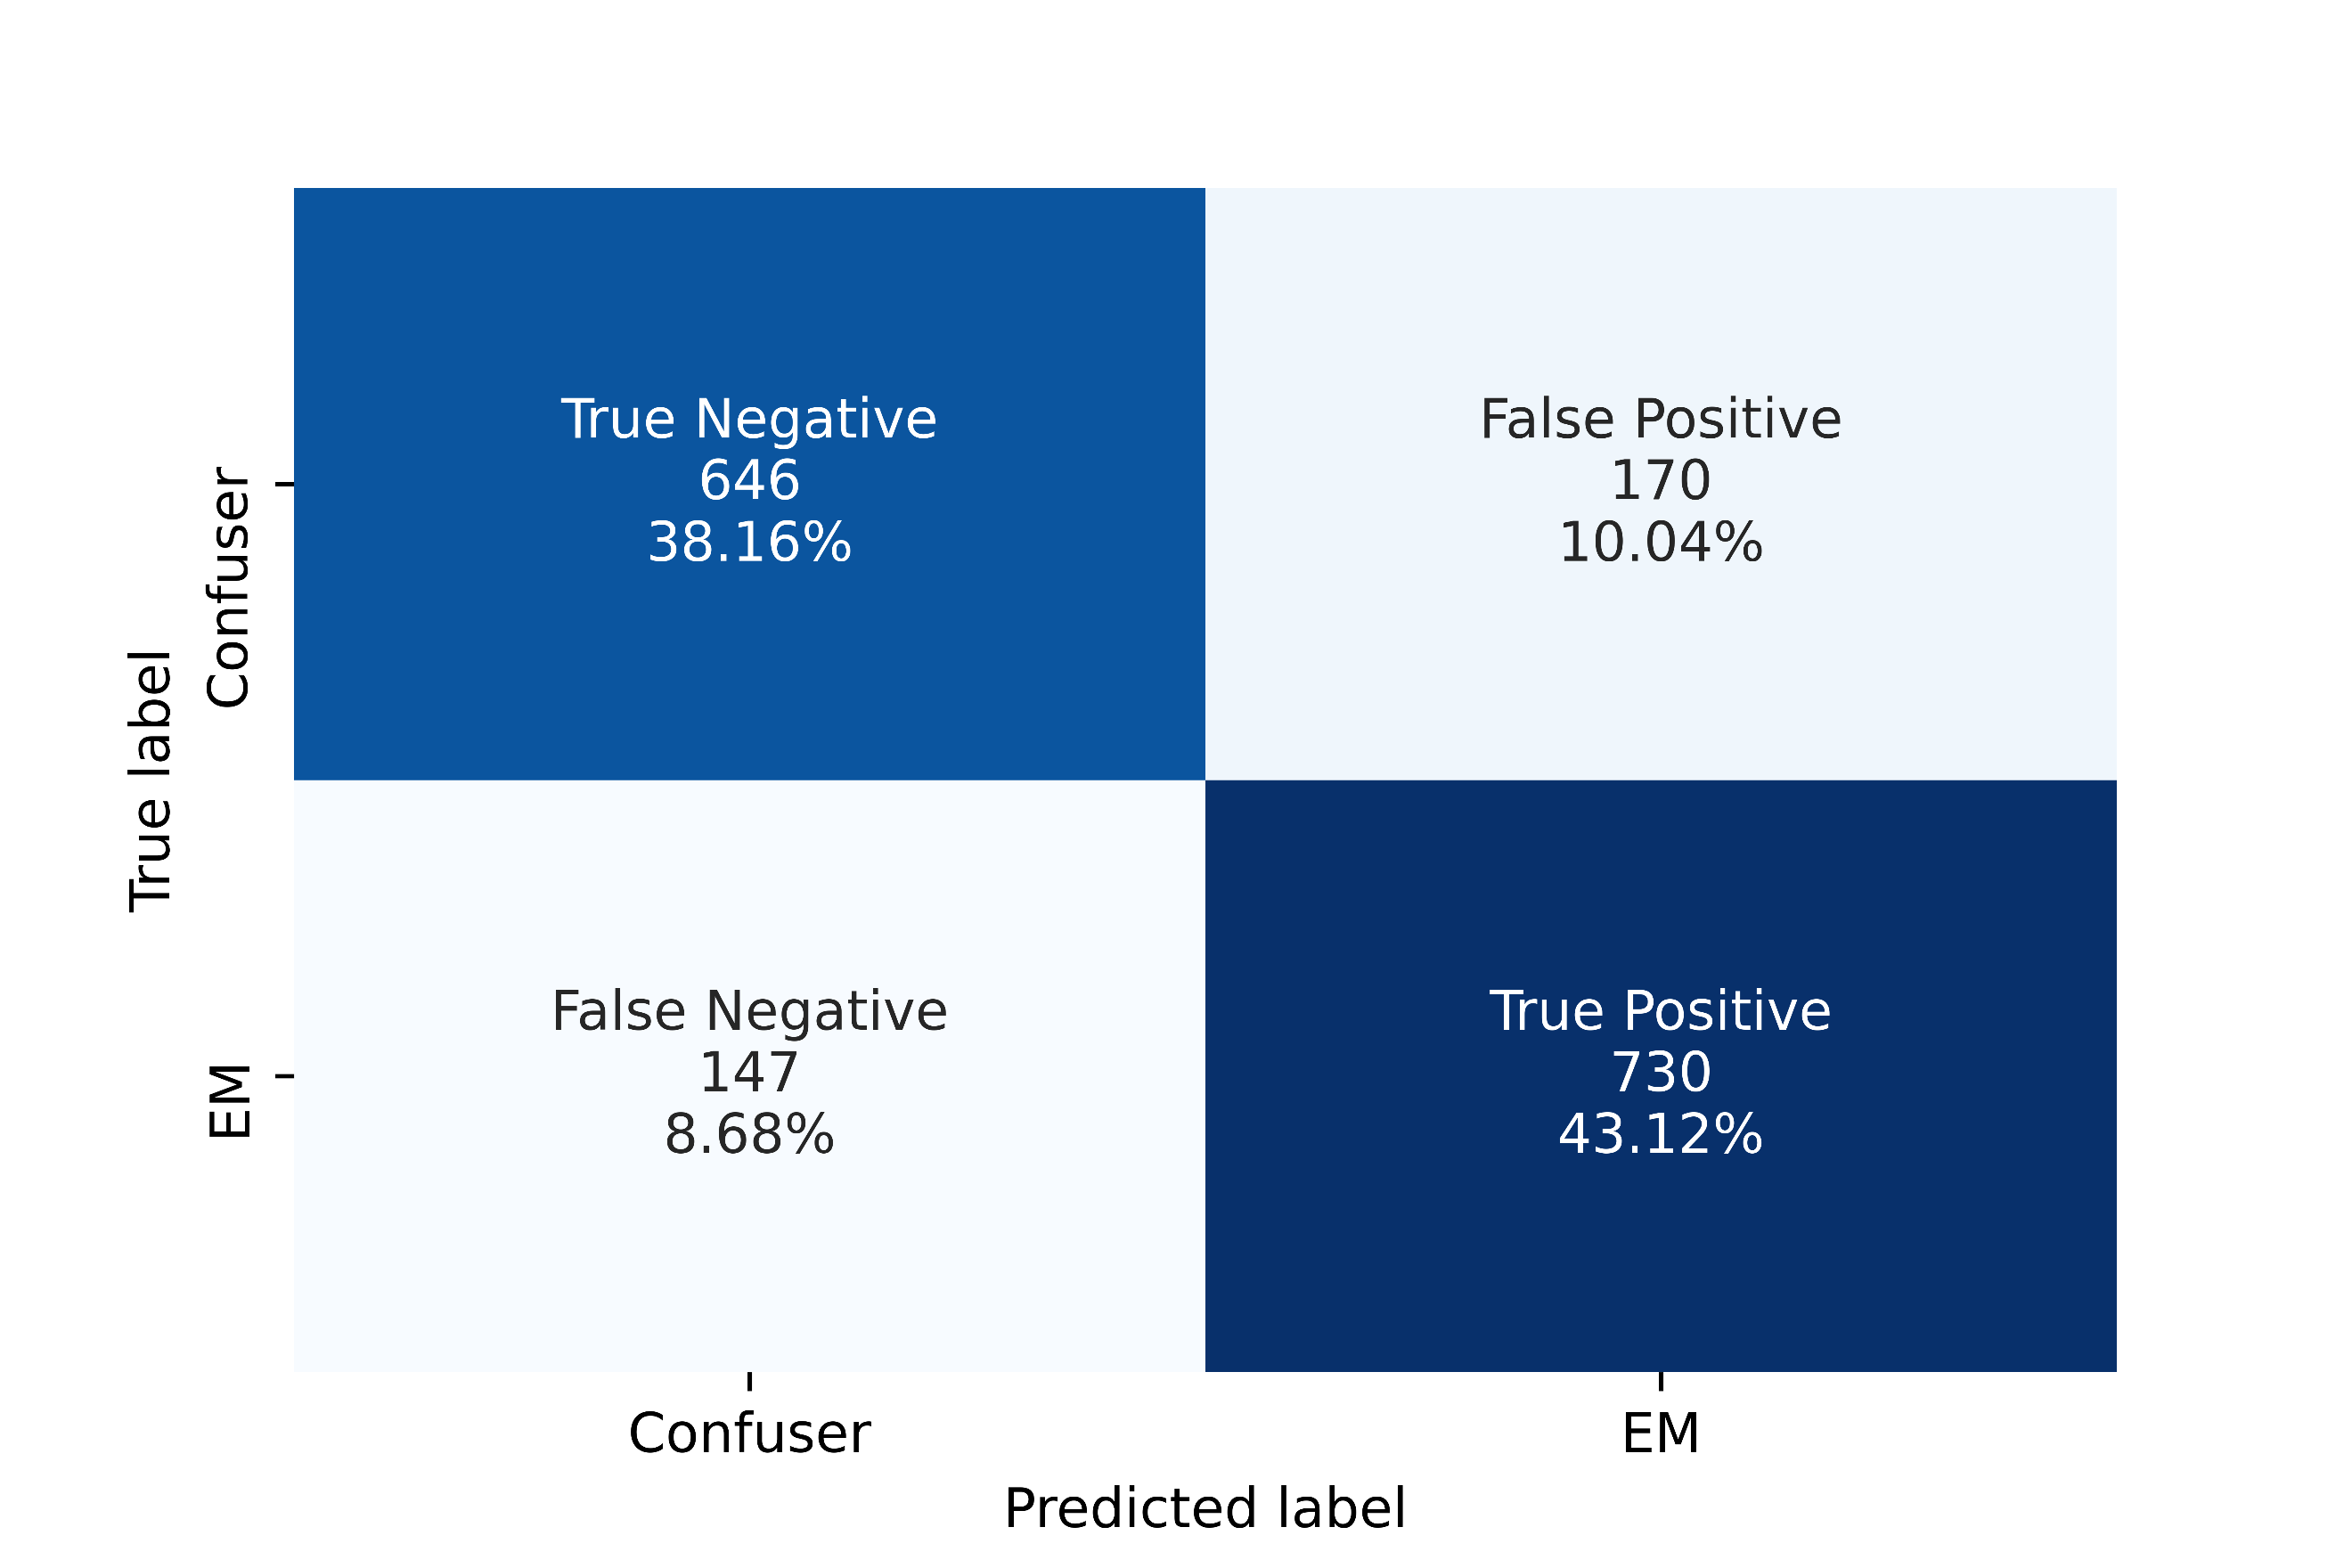
\includegraphics[width=\textwidth,keepaspectratio]{images/Supplement4/image168.png}
		\caption{Confusion matrix.}
	\end{subfigure}
	\caption{Five-fold cross-validation ROC curve and confusion matrix of NASNetMobile-617 model.}
\end{figure}

%%%%%%%%%%%%%%Break%%%%%%%%%%%%%%%%%%%%%%
\vfill\clearpage
\subsection{EfficientNetB0-187}

\begin{table}[h!]
	\centering
	\caption{Five-fold cross-validation performance metrics of EfficientNetB0-187 model.}
	\resizebox{\textwidth}{!}{%
		\begin{tabular}{llllllllllll}
			\toprule
			& \multicolumn{11}{c}{\textbf{Metric}}    \\ \cmidrule(lr){2-12} 
			\multicolumn{1}{l}{\textbf{Fold}} & \rotatebox{45}{Accuracy} & 
			\rotatebox{45}{Sensitivity} & \rotatebox{45}{Specificity} & 
			\rotatebox{45}{Precision} & \rotatebox{45}{NPV} & \rotatebox{45}{MCC} & 
			\rotatebox{45}{Kappa} & \rotatebox{45}{LR$+$} & \rotatebox{45}{LR$-$} & 
			\rotatebox{45}{F1-Score} & \rotatebox{45}{AUC}  \\ \midrule
			fold1          & 81.18 & 82.7  & 79.53 & 81.38 & 80.95 & 0.6229 & 0.6228 & 4.0406 & 0.2175 & 0.8204 & 0.8927 \\
			fold2          & 82.39 & 79.19 & 85.8  & 85.62 & 79.43 & 0.6502 & 0.6483 & 5.5778 & 0.2425 & 0.8228 & 0.8984 \\
			fold3          & 83.53 & 89.02 & 77.64 & 81.05 & 86.81 & 0.6725 & 0.669  & 3.9811 & 0.1415 & 0.8485 & 0.9075 \\
			fold4          & 84.13 & 85.55 & 82.61 & 84.09 & 84.18 & 0.6821 & 0.682  & 4.9191 & 0.1749 & 0.8481 & 0.9239 \\
			fold5          & 84.43 & 89.6  & 78.88 & 82.01 & 87.59 & 0.6903 & 0.6871 & 4.2426 & 0.1319 & 0.8564 & 0.9243 \\\cmidrule(lr){1-12}
			average        & 83.13 & 85.21 & 80.89 & 82.83 & 83.79 & 0.6636 & 0.6618 & 4.5522 & 0.1817 & 0.8392 & 0.9094 \\
			std. deviation & 1.2   & 3.91  & 2.95  & 1.75  & 3.19  & 0.0244 & 0.0237 & 0.6116 & 0.0427 & 0.0147 & 0.0129\\
			\bottomrule
		\end{tabular}%
	}
\end{table}


\begin{figure}[h!]
	\centering
	\begin{subfigure}[b]{0.49\textwidth}
		\centering
		\includegraphics[width=\textwidth,keepaspectratio]{images/Supplement4/image169.png}
		\caption{ROC curve.}
	\end{subfigure}
	\hfill
	\begin{subfigure}[b]{0.49\textwidth}
		\centering
		\includegraphics[width=\textwidth,keepaspectratio]{images/Supplement4/image174.png}
		\caption{Confusion matrix.}
	\end{subfigure}
	\caption{Five-fold cross-validation ROC curve and confusion matrix of EfficientNetB0-187 model.}
\end{figure}

%%%%%%%%%%%%%%Break%%%%%%%%%%%%%%%%%%%%%%
\vfill\clearpage
\subsection{EfficientNetB1-308}

\begin{table}[h!]
	\centering
	\caption{Five-fold cross-validation performance metrics of EfficientNetB1-308 model.}
	\resizebox{\textwidth}{!}{%
		\begin{tabular}{llllllllllll}
			\toprule
			& \multicolumn{11}{c}{\textbf{Metric}}    \\ \cmidrule(lr){2-12} 
			\multicolumn{1}{l}{\textbf{Fold}} & \rotatebox{45}{Accuracy} & 
			\rotatebox{45}{Sensitivity} & \rotatebox{45}{Specificity} & 
			\rotatebox{45}{Precision} & \rotatebox{45}{NPV} & \rotatebox{45}{MCC} & 
			\rotatebox{45}{Kappa} & \rotatebox{45}{LR$+$} & \rotatebox{45}{LR$-$} & 
			\rotatebox{45}{F1-Score} & \rotatebox{45}{AUC}  \\ \midrule
			fold1          & 81.18 & 86.49 & 75.44 & 79.21 & 83.77 & 0.6245 & 0.6216 & 3.5212 & 0.1791 & 0.8269 & 0.8899 \\
			fold2          & 82.99 & 83.24 & 82.72 & 83.72 & 82.21 & 0.6594 & 0.6594 & 4.8159 & 0.2027 & 0.8348 & 0.9193 \\
			fold3          & 82.04 & 89.6  & 73.91 & 78.68 & 86.86 & 0.6452 & 0.6384 & 3.4345 & 0.1408 & 0.8378 & 0.9006 \\
			fold4          & 81.74 & 84.97 & 78.26 & 80.77 & 82.89 & 0.6345 & 0.6335 & 3.9087 & 0.192  & 0.8282 & 0.9063 \\
			fold5          & 84.13 & 84.97 & 83.23 & 84.48 & 83.75 & 0.6822 & 0.6822 & 5.0668 & 0.1806 & 0.8473 & 0.9278 \\\cmidrule(lr){1-12}
			average        & 82.42 & 85.85 & 78.71 & 81.37 & 83.9  & 0.6492 & 0.647  & 4.1494 & 0.179  & 0.835  & 0.9088 \\
			std. deviation & 1.04  & 2.14  & 3.75  & 2.34  & 1.59  & 0.0202 & 0.0214 & 0.6707 & 0.0209 & 0.0074 & 0.0134\\
			\bottomrule
		\end{tabular}%
	}
\end{table}


\begin{figure}[h!]
	\centering
	\begin{subfigure}[b]{0.49\textwidth}
		\centering
		\includegraphics[width=\textwidth,keepaspectratio]{images/Supplement4/image175.png}
		\caption{ROC curve.}
	\end{subfigure}
	\hfill
	\begin{subfigure}[b]{0.49\textwidth}
		\centering
		\includegraphics[width=\textwidth,keepaspectratio]{images/Supplement4/image181.png}
		\caption{Confusion matrix.}
	\end{subfigure}
	\caption{Five-fold cross-validation ROC curve and confusion matrix of EfficientNetB1-308 model.}
\end{figure}

%%%%%%%%%%%%%%Break%%%%%%%%%%%%%%%%%%%%%%
\vfill\clearpage
\subsection{EfficientNetB2-316}

\begin{table}[h!]
	\centering
	\caption{Five-fold cross-validation performance metrics of EfficientNetB2-316 model.}
	\resizebox{\textwidth}{!}{%
		\begin{tabular}{llllllllllll}
			\toprule
			& \multicolumn{11}{c}{\textbf{Metric}}    \\ \cmidrule(lr){2-12} 
			\multicolumn{1}{l}{\textbf{Fold}} & \rotatebox{45}{Accuracy} & 
			\rotatebox{45}{Sensitivity} & \rotatebox{45}{Specificity} & 
			\rotatebox{45}{Precision} & \rotatebox{45}{NPV} & \rotatebox{45}{MCC} & 
			\rotatebox{45}{Kappa} & \rotatebox{45}{LR$+$} & \rotatebox{45}{LR$-$} & 
			\rotatebox{45}{F1-Score} & \rotatebox{45}{AUC}  \\ \midrule
			fold1          & 82.87 & 84.86 & 80.7  & 82.63 & 83.13 & 0.6567 & 0.6564 & 4.3975 & 0.1875 & 0.8373 & 0.9059 \\
			fold2          & 80.6  & 78.61 & 82.72 & 82.93 & 78.36 & 0.6131 & 0.6122 & 4.5483 & 0.2586 & 0.8071 & 0.906  \\
			fold3          & 82.63 & 87.28 & 77.64 & 80.75 & 85.03 & 0.6535 & 0.6512 & 3.9035 & 0.1638 & 0.8389 & 0.897  \\
			fold4          & 82.63 & 88.44 & 76.4  & 80.1  & 86.01 & 0.6547 & 0.6509 & 3.747  & 0.1513 & 0.8407 & 0.9062 \\
			fold5          & 85.03 & 85.55 & 84.47 & 85.55 & 84.47 & 0.7002 & 0.7002 & 5.5094 & 0.1711 & 0.8555 & 0.9224 \\\cmidrule(lr){1-12}
			average        & 82.75 & 84.95 & 80.39 & 82.39 & 83.4  & 0.6556 & 0.6542 & 4.4211 & 0.1865 & 0.8359 & 0.9075 \\
			std. deviation & 1.4   & 3.41  & 3.02  & 1.91  & 2.69  & 0.0276 & 0.0279 & 0.6202 & 0.0379 & 0.0158 & 0.0082\\
			\bottomrule
		\end{tabular}%
	}
\end{table}


\begin{figure}[h!]
	\centering
	\begin{subfigure}[b]{0.49\textwidth}
		\centering
		\includegraphics[width=\textwidth,keepaspectratio]{images/Supplement4/image182.png}
		\caption{ROC curve.}
	\end{subfigure}
	\hfill
	\begin{subfigure}[b]{0.49\textwidth}
		\centering
		\includegraphics[width=\textwidth,keepaspectratio]{images/Supplement4/image187.png}
		\caption{Confusion matrix.}
	\end{subfigure}
	\caption{Five-fold cross-validation ROC curve and confusion matrix of EfficientNetB2-316 model.}
\end{figure}

%%%%%%%%%%%%%%Break%%%%%%%%%%%%%%%%%%%%%%
\vfill\clearpage
\subsection{EfficientNetB3-194}

\begin{table}[h!]
	\centering
	\caption{Five-fold cross-validation performance metrics of EfficientNetB3-194 model.}
	\resizebox{\textwidth}{!}{%
		\begin{tabular}{llllllllllll}
			\toprule
			& \multicolumn{11}{c}{\textbf{Metric}}    \\ \cmidrule(lr){2-12} 
			\multicolumn{1}{l}{\textbf{Fold}} & \rotatebox{45}{Accuracy} & 
			\rotatebox{45}{Sensitivity} & \rotatebox{45}{Specificity} & 
			\rotatebox{45}{Precision} & \rotatebox{45}{NPV} & \rotatebox{45}{MCC} & 
			\rotatebox{45}{Kappa} & \rotatebox{45}{LR$+$} & \rotatebox{45}{LR$-$} & 
			\rotatebox{45}{F1-Score} & \rotatebox{45}{AUC}  \\ \midrule
			fold1          & 83.43 & 87.03 & 79.53 & 82.14 & 85    & 0.6685 & 0.6672 & 4.2519 & 0.1631 & 0.8451 & 0.9149 \\
			fold2          & 81.79 & 76.88 & 87.04 & 86.36 & 77.9  & 0.6409 & 0.6368 & 5.9306 & 0.2656 & 0.8135 & 0.9059 \\
			fold3          & 84.13 & 87.28 & 80.75 & 82.97 & 85.53 & 0.6826 & 0.6816 & 4.5331 & 0.1575 & 0.8507 & 0.9113 \\
			fold4          & 84.13 & 89.02 & 78.88 & 81.91 & 86.99 & 0.684  & 0.6812 & 4.2152 & 0.1392 & 0.8532 & 0.9253 \\
			fold5          & 83.83 & 85.55 & 81.99 & 83.62 & 84.08 & 0.6761 & 0.6759 & 4.7495 & 0.1763 & 0.8457 & 0.9239 \\\cmidrule(lr){1-12}
			average        & 83.46 & 85.15 & 81.64 & 83.4  & 83.9  & 0.6704 & 0.6685 & 4.7361 & 0.1803 & 0.8416 & 0.9163 \\
			std. deviation & 0.87  & 4.28  & 2.9   & 1.6   & 3.14  & 0.0157 & 0.0167 & 0.6283 & 0.0443 & 0.0144 & 0.0074\\
			\bottomrule
		\end{tabular}%
	}
\end{table}


\begin{figure}[h!]
	\centering
	\begin{subfigure}[b]{0.49\textwidth}
		\centering
		\includegraphics[width=\textwidth,keepaspectratio]{images/Supplement4/image188.png}
		\caption{ROC curve.}
	\end{subfigure}
	\hfill
	\begin{subfigure}[b]{0.49\textwidth}
		\centering
		\includegraphics[width=\textwidth,keepaspectratio]{images/Supplement4/image194.png}
		\caption{Confusion matrix.}
	\end{subfigure}
	\caption{Five-fold cross-validation ROC curve and confusion matrix of EfficientNetB3-194 model.}
\end{figure}

%%%%%%%%%%%%%%Break%%%%%%%%%%%%%%%%%%%%%%
\vfill\clearpage
\subsection{EfficientNetB5-444}

\begin{table}[h!]
	\centering
	\caption{Five-fold cross-validation performance metrics of EfficientNetB5-444 model.}
	\resizebox{\textwidth}{!}{%
		\begin{tabular}{llllllllllll}
			\toprule
			& \multicolumn{11}{c}{\textbf{Metric}}    \\ \cmidrule(lr){2-12} 
			\multicolumn{1}{l}{\textbf{Fold}} & \rotatebox{45}{Accuracy} & 
			\rotatebox{45}{Sensitivity} & \rotatebox{45}{Specificity} & 
			\rotatebox{45}{Precision} & \rotatebox{45}{NPV} & \rotatebox{45}{MCC} & 
			\rotatebox{45}{Kappa} & \rotatebox{45}{LR$+$} & \rotatebox{45}{LR$-$} & 
			\rotatebox{45}{F1-Score} & \rotatebox{45}{AUC}  \\ \midrule
			fold1          & 83.43 & 89.73 & 76.61 & 80.58 & 87.33 & 0.6712 & 0.6665 & 3.8359 & 0.1341 & 0.8491 & 0.9119 \\
			fold2          & 85.37 & 90.17 & 80.25 & 82.98 & 88.44 & 0.7092 & 0.7063 & 4.565  & 0.1225 & 0.8643 & 0.9261 \\
			fold3          & 81.74 & 87.28 & 75.78 & 79.47 & 84.72 & 0.6363 & 0.6329 & 3.6032 & 0.1678 & 0.832  & 0.8833 \\
			fold4          & 83.53 & 83.24 & 83.85 & 84.71 & 82.32 & 0.6706 & 0.6704 & 5.1543 & 0.1999 & 0.8397 & 0.9236 \\
			fold5          & 84.43 & 83.82 & 85.09 & 85.8  & 83.03 & 0.6887 & 0.6885 & 5.6226 & 0.1902 & 0.848  & 0.9242 \\\cmidrule(lr){1-12}
			average        & 83.7  & 86.85 & 80.32 & 82.71 & 85.17 & 0.6752 & 0.6729 & 4.5562 & 0.1629 & 0.8466 & 0.9138 \\
			std. deviation & 1.21  & 2.89  & 3.73  & 2.39  & 2.38  & 0.024  & 0.0245 & 0.7645 & 0.0303 & 0.0108 & 0.0161\\
			\bottomrule
		\end{tabular}%
	}
\end{table}


\begin{figure}[h!]
	\centering
	\begin{subfigure}[b]{0.49\textwidth}
		\centering
		\includegraphics[width=\textwidth,keepaspectratio]{images/Supplement4/image195.png}
		\caption{ROC curve.}
	\end{subfigure}
	\hfill
	\begin{subfigure}[b]{0.49\textwidth}
		\centering
		\includegraphics[width=\textwidth,keepaspectratio]{images/Supplement4/image200.png}
		\caption{Confusion matrix.}
	\end{subfigure}
	\caption{Five-fold cross-validation ROC curve and confusion matrix of EfficientNetB5-444 model.}
\end{figure}

%%%%%%%%%%%%%%Break%%%%%%%%%%%%%%%%%%%%%%
\vfill\clearpage
\subsection{EfficientNetV2S-413}

\begin{table}[h!]
	\centering
	\caption{Five-fold cross-validation performance metrics of EfficientNetV2S-413 model.}
	\resizebox{\textwidth}{!}{%
		\begin{tabular}{llllllllllll}
			\toprule
			& \multicolumn{11}{c}{\textbf{Metric}}    \\ \cmidrule(lr){2-12} 
			\multicolumn{1}{l}{\textbf{Fold}} & \rotatebox{45}{Accuracy} & 
			\rotatebox{45}{Sensitivity} & \rotatebox{45}{Specificity} & 
			\rotatebox{45}{Precision} & \rotatebox{45}{NPV} & \rotatebox{45}{MCC} & 
			\rotatebox{45}{Kappa} & \rotatebox{45}{LR$+$} & \rotatebox{45}{LR$-$} & 
			\rotatebox{45}{F1-Score} & \rotatebox{45}{AUC}  \\ \midrule
			fold1          & 81.79 & 81.61 & 81.99 & 83.04 & 80.49 & 0.6356 & 0.6355 & 4.5307 & 0.2243 & 0.8232 & 0.9097 \\
			fold2          & 83.58 & 80.92 & 86.42 & 86.42 & 80.92 & 0.6734 & 0.672  & 5.959  & 0.2207 & 0.8358 & 0.9106 \\
			fold3          & 80.84 & 83.82 & 77.64 & 80.11 & 81.7  & 0.6163 & 0.6156 & 3.7484 & 0.2085 & 0.8192 & 0.8917 \\
			fold4          & 83.23 & 88.44 & 77.64 & 80.95 & 86.21 & 0.6662 & 0.6631 & 3.9552 & 0.1489 & 0.8453 & 0.927  \\
			fold5          & 87.43 & 87.86 & 86.96 & 87.86 & 86.96 & 0.7482 & 0.7482 & 6.736  & 0.1396 & 0.8786 & 0.9328 \\\cmidrule(lr){1-12}
			average        & 83.37 & 84.53 & 82.13 & 83.68 & 83.26 & 0.6679 & 0.6669 & 4.9859 & 0.1884 & 0.8404 & 0.9144 \\
			std. deviation & 2.26  & 3.11  & 4.05  & 3.02  & 2.76  & 0.0451 & 0.0453 & 1.1671 & 0.0365 & 0.0212 & 0.0145\\
			\bottomrule
		\end{tabular}%
	}
\end{table}


\begin{figure}[h!]
	\centering
	\begin{subfigure}[b]{0.49\textwidth}
		\centering
		\includegraphics[width=\textwidth,keepaspectratio]{images/Supplement4/EfficientNetV2SHAMIMGCOPYWEIGHTEC413_MultiROC.png}
		\caption{ROC curve.}
	\end{subfigure}
	\hfill
	\begin{subfigure}[b]{0.49\textwidth}
		\centering
		\includegraphics[width=\textwidth,keepaspectratio]{images/Supplement4/EfficientNetV2SHAMIMGCOPYWEIGHTEC413_Combined_CM.png}
		\caption{Confusion matrix.}
	\end{subfigure}
	\caption{Five-fold cross-validation ROC curve and confusion matrix of EfficientNetV2S-413 model.}
\end{figure}

%%%%%%%%%%%%%%Break%%%%%%%%%%%%%%%%%%%%%%
\vfill\clearpage
\subsection{ConvNeXtTiny-120}

\begin{table}[h!]
	\centering
	\caption{Five-fold cross-validation performance metrics of ConvNeXtTiny-120 model.}
	\resizebox{\textwidth}{!}{%
		\begin{tabular}{llllllllllll}
			\toprule
			& \multicolumn{11}{c}{\textbf{Metric}}    \\ \cmidrule(lr){2-12} 
			\multicolumn{1}{l}{\textbf{Fold}} & \rotatebox{45}{Accuracy} & 
			\rotatebox{45}{Sensitivity} & \rotatebox{45}{Specificity} & 
			\rotatebox{45}{Precision} & \rotatebox{45}{NPV} & \rotatebox{45}{MCC} & 
			\rotatebox{45}{Kappa} & \rotatebox{45}{LR$+$} & \rotatebox{45}{LR$-$} & 
			\rotatebox{45}{F1-Score} & \rotatebox{45}{AUC}  \\ \midrule
			fold1          & 84.78 & 90.23 & 78.88 & 82.2  & 88.19 & 0.6975 & 0.6939 & 4.2727 & 0.1239 & 0.8603 & 0.9227 \\
			fold2          & 83.88 & 83.82 & 83.95 & 84.8  & 82.93 & 0.6774 & 0.6774 & 5.2223 & 0.1928 & 0.843  & 0.9188 \\
			fold3          & 80.54 & 81.5  & 79.5  & 81.03 & 80    & 0.6102 & 0.6102 & 3.9764 & 0.2327 & 0.8127 & 0.8897 \\
			fold4          & 86.83 & 90.17 & 83.23 & 85.25 & 88.74 & 0.7369 & 0.7356 & 5.377  & 0.1181 & 0.8764 & 0.9319 \\
			fold5          & 85.03 & 87.86 & 81.99 & 83.98 & 86.27 & 0.7005 & 0.6997 & 4.8778 & 0.1481 & 0.8588 & 0.9283 \\\cmidrule(lr){1-12}
			average        & 84.21 & 86.72 & 81.51 & 83.45 & 85.23 & 0.6845 & 0.6834 & 4.7452 & 0.1631 & 0.8502 & 0.9183 \\
			std. deviation & 2.07  & 3.5   & 2     & 1.6   & 3.31  & 0.0418 & 0.0412 & 0.5401 & 0.0436 & 0.0215 & 0.015 \\
			\bottomrule
		\end{tabular}%
	}
\end{table}


\begin{figure}[h!]
	\centering
	\begin{subfigure}[b]{0.49\textwidth}
		\centering
		\includegraphics[width=\textwidth,keepaspectratio]{images/Supplement4/ConvNextTinyHAMIMGCOPYWEIGHTEC120_MultiROC.png}
		\caption{ROC curve.}
	\end{subfigure}
	\hfill
	\begin{subfigure}[b]{0.49\textwidth}
		\centering
		\includegraphics[width=\textwidth,keepaspectratio]{images/Supplement4/ConvNextTinyHAMIMGCOPYWEIGHTEC120_Combined_CM.png}
		\caption{Confusion matrix.}
	\end{subfigure}
	\caption{Five-fold cross-validation ROC curve and confusion matrix of ConvNeXtTiny-120 model.}
\end{figure}